\documentclass[a4paper,11pt,twoside]{include/ThesisStyle}
%\documentclass[10pt,twoside]{include/ThesisStyle}

% =============================================================================


\newcommand{\thesistitle}{Virtualization Support for Application\\Runtime Specialization and Extension}
\newcommand{\thesisauthor}{Guillermo Polito}
\newcommand{\thesisurl}{http://rmod.inria.fr/}
\newcommand{\thesissubtitle}{}
\newcommand{\thesisdate}{13. Avril 2015}

% =============================================================================

\usepackage[utf8]{inputenc}
\usepackage[T1]{fontenc}

% modify the default page geometry
\usepackage[left=1.7in,right=1.5in,top=2cm,bottom=2cm,includefoot,includehead,headheight=13.6pt]{geometry}
%\usepackage[bottom=1cm,top=1cm, includefoot,includehead, headheight=5pt, paperwidth=6in, paperheight=9in]{geometry}

% =============================================================================
%\usepackage{algorithm}
\usepackage{alltt} % math support in verbatim text
\usepackage{amsfonts}
\usepackage{amsmath}
\usepackage{amssymb}
\usepackage{bold-extra} % bold support for small caps 
\usepackage[hypcap]{caption} % with hyperref point to the head of the pic
\usepackage{caption}
\usepackage{chngpage} % allows for temporary adjustment of side margins
\usepackage{cite}
\usepackage{color} % custom colors for text
\usepackage{enumerate} % enable enumerated lists
\usepackage[shortlabels]{enumitem} % enables [noitemsep,nolistsep] for more compact lists and various flavours of enum labels
\usepackage{booktabs} % used for \midrule
\usepackage{fancyhdr} % Fancy Header and Footer
\usepackage{float}      % for the strong here [H] of figures
\usepackage{graphicx} % extended arguments for \in­clude­graph­ics
\usepackage[htt]{hyphenat} % enable hyphenation of \textt + custom hypenation rules for words
% \usepackage{hyperref} see at the end of the header.tex
\usepackage{algorithm2e}
\usepackage{ifthen} % support boolean "branches" => enables conditional macros
\usepackage{tgtermes} % tex gyre thermes font
\usepackage{multirow} % fancy stuff for tables: multirow, bigdelim, bigstrut
\usepackage{rotating} % Sideways of figures & tables
\usepackage{slantsc} % http://ctan.org/pkg/slantsc enable fake italic small caps in fonts that do not have native support for this
\usepackage{stmaryrd} % St Mary Road symbols for theoretical computer science
\usepackage{subcaption}
\usepackage{url}    % add url/link support  
\usepackage{wrapfig} % suppport for figures with text wrapped around 
\usepackage{xspace}
\usepackage[normalem]{ulem} % for \sout
\usepackage[table,svgnames]{xcolor}
\usepackage{tabularx}
\usepackage{tablefootnote}
\usepackage{pifont} %  Access to PostScript standard Symbol and Dingbats fonts

\usepackage{float,lscape}

% Font choices (I need real smallcaps!)
%\usepackage{libertine}
%\usepackage[osf]{mathpazo} % palatino with real small caps and oldstyle numbers
\usepackage{tgpagella} % Use TeX Gyre Pagella with real small caps (normal + bold)
\usepackage{tgcursor} % fixed wifth font TeX Gyre Cursor (Courrier Style)

% =============================================================================
% enable decimal columns in tables
\usepackage{dcolumn}
% define a new columntype "d" for decimal aligned numbers which takes as argument
% the number of decimal places to be displayed
\newcolumntype{d}[1]{D{.}{.}{#1} }

%the argument for d specifies the maximum number of decimal places
%\begin{tabular}{l r c d{1} }
%Left&Right&Center&\mathrm{Decimal}\\
%1&2&3&4\\
%11&22&33&44\\
%1.1&2.2&3.3&4.4\\
%\end{tabular}
% =============================================================================
% support proper SI units in latex: for instance \num{0.235+-0.005} is properly formatted as 0.235(5)
\usepackage{siunitx} 
% setup the si units package globally
\sisetup{
	separate-uncertainty = true % show the +/- for uncertainty, computer scienticts have no clue about the 0.2352(66) notion
}


% =============================================================================
 % environment hooks and patching:
\usepackage{etoolbox}

% Helper command for reducing spaces after certain environment (see below...)
\makeatletter
% uncomment the following if you don't want \clubpenalty\@M ...
% \let\nearly@afterheading\@afterheading
% \patchcmd\nearly@afterheading
%   {\@M}% original temporary setting for \clubpenalty replaced by ...
%   {\@clubpenalty}% ... or whichever value you deem right
%   {}{}
% ... and use \nearly@afterheading instead of \@afterheading here:
\newcommand*\NoIndentAfterEnv[1]{%
  \AfterEndEnvironment{#1}{\par\@afterindentfalse\@afterheading}}
\makeatother

% Disable indentation after a certain environment: \NoIndentAfterEnv{itemize}
% note that this might break the space for the paragraph follwing such a modified one
%\NoIndentAfterEnv{itemize}
%\NoIndentAfterEnv{enumerate}
%\NoIndentAfterEnv{description}
%\NoIndentAfterEnv{table}
%\NoIndentAfterEnv{figure}

%\renewcommand*\arraystretch{1.2} % modify the line spacing in tables

% globally reduce the space between list items
\newlength{\wideitemsep}
\setlength{\wideitemsep}{.5\itemsep}
\addtolength{\wideitemsep}{-3pt}
\let\olditem\item
\renewcommand{\item}{\setlength{\itemsep}{\wideitemsep}\olditem}


% =============================================================================
% Settings to add a small (mini) Table of contents at the beginning of each chapter
\usepackage[nottoc, notlof, notlot]{tocbibind}
\usepackage[tight]{minitoc} % tight=single line spacing
\setcounter{minitocdepth}{2}
% change the minitoc fonts
\renewcommand{\mtcfont}{\small\normalfont} 
\renewcommand{\mtcSfont}{\mtcfont} 
\renewcommand{\mtifont}{\Large\bf} % use the same font as for the section font for the title of the contents
\nomtcrule % no visual minitoc rule
\mtcindent=2pt % indent just enough to make it visually look aligned

\setcounter{secnumdepth}{3}
\setcounter{tocdepth}{2}
  
% =============================================================================
% Fancy Header Style Options

\pagestyle{fancy}                       % Sets fancy header and footer
\fancyfoot{}                            % Delete current footer settings

%\renewcommand{\chaptermark}[1]{         % Lower Case Chapter marker style
%  \markboth{\chaptername\ \thechapter.\ #1}}{}} %

%\renewcommand{\sectionmark}[1]{         % Lower case Section marker style
%  \markright{\thesection.\ #1}}         %

\fancyhead[LE,RO]{\thepage}					% Page number (boldface) on the left on even
											% pages and on the right on odd pages
\fancyhead[RE]{\nouppercase{\leftmark}}		% Chapter on the right on even pages
\fancyhead[LO]{\nouppercase{\rightmark}}	% Section on the left on odd pages

\let\headruleORIG\headrule
\renewcommand{\headrule}{\color{black} \headruleORIG}
\renewcommand{\headrulewidth}{0pt}
\usepackage{colortbl}
\arrayrulecolor{black}

\fancypagestyle{plain}{
  \fancyhead{}
  \fancyfoot{}
  \renewcommand{\headrulewidth}{0pt}
}

% Clear Header Style on the Last Empty Odd pages
\makeatletter

\def\cleardoublepage{\clearpage\if@twoside \ifodd\c@page\else%
  \hbox{}%
  \thispagestyle{empty}%              % Empty header styles
  \newpage%
  \if@twocolumn\hbox{}\newpage\fi\fi\fi}

\makeatother

% centered page environment
\newenvironment{vcenterpage}
	{\newpage\vspace*{\fill}\thispagestyle{empty}\renewcommand{\headrulewidth}{0pt}}
	{\vspace*{\fill}}
	
% automatically insert a period at the end of a paragraph title.
\let\originalparagraph\paragraph
\renewcommand{\paragraph}[2][.]{\originalparagraph{#2#1\!\!\!\!}}

% enable french spacing: 1 space after a dot instead of the 2 in english
\frenchspacing

%=============================================================================
\usepackage{needspace}
% \needlines{3} ensures that the following 3 lines will be on the same page
% typically used in code examples where arbitrary broken up parts are hard to read
\newcommand{\needlines}[1]{\Needspace{#1\baselineskip}}

\definecolor{source}{gray}{0.95}
\definecolor{light-gray}{rgb}{0.8,0.8,0.8}
\definecolor{comment}{rgb}{0.35,0.35,0.35}
\definecolor{string}{rgb}{0,0.4,0}
\definecolor{darkRed}{rgb}{0.5,0,0}
\definecolor{darkBlue}{rgb}{0,0,0.3}
\definecolor{darkCyan}{rgb}{0,0.3,0.3}

% source code formatting
\usepackage{listings}
% global settings for source code listing package
\lstset{
    basicstyle=\ttfamily,
    showspaces=false,
    showstringspaces=false,
    lineskip=-0.1pt,
    stepnumber=2,
    numberfirstline=true,
    captionpos=b,
    emphstyle=\bf\ttfamily,
    columns=fullflexible}

% define Smalltalk like grammar for the listing package
\lstdefinelanguage{ST}{
    keywordsprefix=\#,
    morekeywords=[0]{true,false,nil},
    morekeywords=[1]{self,super,thisContext},
    morekeywords=[2]{ifTrue:,ifFalse:,whileTrue:,whileFalse:,and:,or:,xor:,not:,by:,timesRepeat:},
	morekeywords=[3]{Benzo,FFI},
    sensitive=true,
    morecomment=[s]{"}{"},
    morestring=[d]',
    escapechar={!},
    alsoletter={., :, -, =, +, <},
    moredelim=**[is][\itshape]{/+}{+/},
    literate=
        {~}{{$\sim$}}1
        {-}{{\sf -\hspace{-0.13em}-}}1  % the goal is to make - the same width as +
        {+}{\raisebox{0.08ex}{+}}1		% and to raise + off the baseline to match V
        , % Don't forget the comma at the end!
    style=STStyle
}
\lstdefinestyle{STStyle}{
    tabsize=4,
    %frame=leftline,
    %frame=bl,
    %framerule=2pt,
    %rulecolor=\color{gray},
    %backgroundcolor=\color{white},
    %backgroundcolor=\usebeamercolor[bg]{listing},
    basicstyle=\ttfamily,
    keywordstyle=\bfseries\ttfamily,
    %stringstyle=\color{orange},
    stringstyle=\mdseries\slshape,
    %commentstyle=\it\rmfamily\color{darkgray}, 
    commentstyle=\mdseries\slshape\color{darkgray},
    %commentstyle=\mdseries\slshape,
    emphstyle=\bf\ttfamily,
    escapeinside={!}{!},
	%backgroundcolor=\color{source},
    %emphstyle={[2]\color{red}},
    %emphstyle={[3]\color{blue}\bf},
    %emphstyle={[4]\color{blue}},
    keepspaces=true
} 

%\lstnewenvironment{javacode}  [1][]{\lstset{language=java,#1}\needlines{#2}}{} 
%\lstnewenvironment{pythoncode}[2][]{\lstset{language=python,#1}\needlines{#2}}{}
\lstnewenvironment{stcode}    [2][]{\lstset{language=ST,#1}\needlines{#2}}{}
\lstnewenvironment{ccode}     [2][]
    {\lstset{language=C,numbers=left,escapechar=\$,numberstyle=\tiny,#1}\needlines{#2}}{}

% code environment with line numbers and support for \needlines which keeps a
% given number of lines of the code together (see needline comment above)
\lstnewenvironment{numstcode} [2][]
    {\lstset{language=ST,numbers=left,numberstyle=\tiny,numbersep=5pt,#1}\needlines{#2}}{}
\lstnewenvironment{numstcodecont} [2][]
    {\lstset{language=ST,numbers=left,numberstyle=\tiny,numbersep=5pt,firstnumber=last#1}\needlines{#2}}{}

\newcommand{\lst}[1]{{\tt #1}}

% Use this only in special situations where \ct does not work
% (within Section headings ...):
%\newcommand{\lct}[1]{{\textsf{\textup{#1}}}}
% Code environments
%\lstnewenvironment{code}{%
%	\lstset{%
%		% frame=lines,
%		frame=single,
%		framerule=0pt,
%		mathescape=false,
%		basicstyle=\fontsize{10}{12}\selectfont\ttfamily
%	}
%}{}

%\newenvironment{code}
%    {\begin{alltt}\sffamily}
%    {\end{alltt}\small}

\definecolor{source}{gray}{1}
\definecolor{unusedsource}{gray}{0.85}
%\newcommand{\myCommentStyle}[1]{{\footnotesize\sffamily\color{gray!100!white} #1}}
\newcommand{\myCommentStyle}[1]{{\footnotesize\sffamily\color{black!100!white} #1}}
 
% my string style
%\newcommand{\myStringStyle}[1]{{\footnotesize\sffamily\color{violet!100!black} #1}}
\newcommand{\myStringStyle}[1]{{\footnotesize\sffamily\color{black!100!black} #1}}
 
% my symbol style
\newcommand{\mySymbolStyle}[1]{{\footnotesize\sffamily\color{violet!100!black} #1}}
%\newcommand{\mySymbolStyle}[1]{{\footnotesize\sffamily\color{black!100!black} #1}}
 
% my keyword style
%\newcommand{\myKeywordStyle}[1]{{\footnotesize\sffamily\color{green!70!black} #1}}
\newcommand{\myKeywordStyle}[1]{{\footnotesize\sffamily\color{black!70!black} #1}}
 
% my global style
%\newcommand{\myGlobalStyle}[1]{{\footnotesize\sffamily\color{blue!100!black} #1}}
\newcommand{\myGlobalStyle}[1]{{\footnotesize\sffamily\color{black!100!black} #1}}
 
% my number style
%\newcommand{\myNumberStyle}[1]{{\footnotesize\sffamily\color{brown!100!black} #1}}
\newcommand{\myNumberStyle}[1]{{\footnotesize\sffamily\color{black!100!black} #1}}
 
\lstset{
language={},
% characters
tabsize=3,
escapechar={!},
keepspaces=true,
breaklines=true,
alsoletter={\#},
literate={\$}{{{\$}}}1,
breakautoindent=true,
columns=fullflexible,
showstringspaces=false,
% background
frame=single,
aboveskip=1em, % automatic space before
framerule=0pt,
basicstyle=\footnotesize\sffamily\color{black},
keywordstyle=\myKeywordStyle,% keyword style
commentstyle=\myCommentStyle,% comment style
frame=single,%
backgroundcolor=\color{source},
% numbering
stepnumber=1,
numbersep=10pt,
numberstyle=\tiny,
numberfirstline=true,
% caption
captionpos=b,
% formatting (html)
moredelim=[is][\bfseries]{&lt;b&gt;}{&lt;/b&gt;},
moredelim=[is][\textit]{&lt;i&gt;}{&lt;/i&gt;},
moredelim=[is][\underbar]{&lt;u&gt;}{&lt;/u&gt;},
moredelim=[is][\color{red}\uwave]{&lt;wave&gt;}{&lt;/wave&gt;},
moredelim=[is][\color{red}\sout]{&lt;del&gt;}{&lt;/del&gt;},
moredelim=[is][\color{blue}\underbar]{&lt;ins&gt;}{&lt;/ins&gt;},
% smalltalk stuff
morecomment=[s][\myCommentStyle]{"}{"},
% morecomment=[s][\myvs]{|}{|},
morestring=[b][\myStringStyle]',
moredelim=[is][]{&lt;sel&gt;}{&lt;/sel&gt;},
moredelim=[is][]{&lt;rcv&gt;}{&lt;/rcv&gt;},
moredelim=[is][\itshape]{&lt;symb&gt;}{&lt;/symb&gt;},
moredelim=[is][\scshape]{&lt;class&gt;}{&lt;/class&gt;},
morekeywords={true,false,nil,self,super,thisContext},
identifierstyle=\idstyle,
}

\makeatletter
\newcommand*\idstyle[1]{%
\expandafter\id@style\the\lst@token{#1}\relax%
}
\def\id@style#1#2\relax{%
\ifnum\pdfstrcmp{#1}{\#}=0%
% this is a symbol
\mySymbolStyle{\the\lst@token}%
\else%
\edef\tempa{\uccode`#1}%
\edef\tempb{`#1}%
\ifnum\tempa=\tempb%
% this is a global
\myGlobalStyle{\the\lst@token}%
\else%
\the\lst@token%
\fi%
\fi%
}

\newcommand{\unusedcode}[1]{\colorbox{unusedsource}{\makebox[\columnwidth][l]{#1}}}

\makeatother
%\newcommand{\ct}{\lstinline[backgroundcolor=\color{white}]}
%\newcommand{\needlines}[1]{\Needspace{#1\baselineskip}}
\newcommand{\lct}{\texttt}


 
\lstnewenvironment{code}{%
 \lstset{%
 %frame=lines,
 frame=single,
 framerule=0pt,
 mathescape=false,
 moredelim=**[is][{\btHL[fill=green!30,draw=red,dashed,thin]}]{@}{@},
 numbers=left
 }%
 \noindent%
 \minipage{\linewidth}%
}{%
 \endminipage%
}%

\renewcommand{\lstlistingname}{Code Example}

% =============================================================================
% support for annotations direclty in the latex sources
\newboolean{showcomments}
% create a boolean to enable/disable comments (use \setboolean{showcomments}{false} 
% for instance in the main file)
\setboolean{showcomments}{true}
\newcommand\ifshowcomment[2]{\ifthenelse{\boolean{showcomments}}{#1}{#2}}
% used to deal with the spaces inserted by hidden comments
\newcommand\commentbackspace{\!\!\!} %\!\!\!\!\!

% please rephrase
\newcommand\ugh[1]{
	\ifshowcomment
		{\textcolor{red}{\uwave{#1}}}
		{#1}}
% please insert
\newcommand\ins[1]{
	\ifshowcomment
		{\textcolor{blue}{\uline{#1}}}
		{#1}}
% please delete							
\newcommand\del[1]{
	\ifshowcomment
		{\textcolor{red}{\sout{#1}}}
		{\commentbackspace}}
% please change
\newcommand\chg[2]{ %
	\ifshowcomment
		{\textcolor{red}{\sout{#1}}{\ra} %
		\textcolor{blue}{\uline{#2}}} %
		{\commentbackspace}}
% comment with color
\newcommand\nbc[3]{ %
	\ifshowcomment{ %
		{\colorbox{#3}{\bfseries\sffamily\scriptsize\textcolor{white}{#1}}}{\color{#3}
			\sf\small$\blacktriangleright$
			{\itshape #2}
			$\blacktriangleleft$}}
		{\commentbackspace}}



\newcommand\nb[2]  {\nbc{#1}{#2}{orange}}
\newcommand\fix[1] {\nb{FIX}{#1}}
\newcommand\todo[1]{\nb{TO DO}{#1}}
\newcommand{\ct}[1]{{\textsf{#1}}\xspace}

\newcommand{\objectspace}{Object Space\xspace}
\newcommand{\objectspaces}{Object Spaces\xspace}

\newtheorem{definition}{Definition}

% shortcuts for comments by reviewers
\newcommand\cb[1]{\nbc{CB}{#1}{purple}} % camillo bruni
\newcommand\lf[1]{\nbc{LF}{#1}{purple}} % luc fabresse
%\newcommand\nb[1]{\nbc{NB}{#1}{purple}} % noury
\newcommand\gp[1]{\nbc{GP}{#1}{purple}} % guille
\newcommand\sd[1]{\nbc{SD}{#1}{orange}} % stephane ducasse
\newcommand\is[1]{\nbc{IS}{#1}{gray}}   % igor stasenko
\newcommand\sm[1]{\nbc{SM}{#1}{olive}}  % stefan marr
%\newcommand\ct[1]{\nbc{CT}{#1}{teal}}   % camille tereul
\newcommand\md[1]{\nbc{MD}{#1}{blue}}   % marcus denker
\newcommand\dc[1]{\nbc{DC}{#1}{green}}  % damien cassou
\newcommand\lt[1]{\nbc{LT}{#1}{green}}  % laurence tratt
\newcommand\cd[1]{\nbc{CD}{#1}{teal}}   % christophe dony
\newcommand\gt[1]{\nbc{GT}{#1}{blue}}   % gael thomas

% =============================================================================
\usepackage[pagebackref,hyperindex=true]{hyperref}

% Links in pdf should be black
\definecolor{linkcol}{rgb}{0.0, 0.0, 0.0} 
\definecolor{citecol}{rgb}{0.0, 0.0, 0.0} 

% Change this to change the informations included in the pdf file
% See hyperref documentation for information on those parameters
\hypersetup {
	bookmarksopen=true,
	pdftitle=\thesistitle,
	pdfauthor=\thesisauthor, 
	pdfsubject="", %subject of the document
	pdfhighlight=/O, %effect of clicking on a link
	colorlinks=false,
	pdfpagemode=UseNone,
	pdfpagelayout=SinglePage,
	pdffitwindow=true,
	linkcolor=linkcol,
	citecolor=citecol,
	urlcolor=linkcol
}

% =============================================================================
% Reference macros for common elements
% use \figlabel{myKey} instead of \label{fig:myKey} and the according \figref below
\newcommand{\figlabel}[1] {\label{fig:#1}}
\newcommand{\chaplabel}[1]{\label{chap:#1}}
\newcommand{\seclabel}[1] {\label{sec:#1}}
\newcommand{\tablabel}[1] {\label{tab:#1}}
\newcommand{\lstlabel}[1] {\label{lst:#1}}

\newcommand{\figref}[1] {\hyperref[fig:#1]{Figure}~\ref{fig:#1}}
\newcommand{\chapref}[1]{\hyperref[chap:#1]{Chapter}~\ref{chap:#1}}
\newcommand{\secref}[1] {\hyperref[sec:#1]{Section}~\ref{sec:#1}}
\newcommand{\tabref}[1] {\hyperref[tab:#1]{Table}~\ref{tab:#1}}
\newcommand{\lstref}[1] {\hyperref[lst:#1]{Listing}~\ref{lst:#1}}

% Macro for adding at the same time a link to the final pdf and add a footnote with 
% the url useful for printed versions: \urlfootnote{Google}{http://google.com/}
\newcommand{\urlfootnote}[2] {\href{#2}{#1}\footnote{\url{#2}}}

\newcommand{\commented}[1]{}

% custom Introduction section, slightly pushed left to visually align with the following paragraph
\newcommand{\introduction}{\section*{\hspace{-1pt}Introduction}} 

\newcommand{\bs}    {\symbol{'134}} % backslash
\newcommand{\us}    {\symbol{'137}} % underscore
\newcommand{\ttt}[1]{\texttt{#1}}
\newcommand{\ie}    {\emph{i.e.},\xspace}
\newcommand{\eg}    {\emph{e.g.},\xspace}
\newcommand{\etal}  {\emph{et al.}\xspace}
\newcommand{\ns}    {\!\!\!\!} %big negative space
\newcommand{\cnull} {\textbackslash0\xspace}
\renewcommand{\epsilon}{\varepsilon}


% italic quotes
%\let\oldquote\quote
%\let\oldendquote\endquote
%\renewenvironment{quote}
%	{\oldquote\itshape}
%	{\oldendquote}
	
% =============================================================================
% Add custom hypenation rules for difficult words here:
\hyphenation{tool-chain pipe-line lan-guage lan-guage-side ge-ne-ric bind-ing bind-ings pri-mi-tive pri-mi-tives Na-tive-Bo-ost}

% the following settings limit a bit the warnings latex spits out to focus on the
% really bad ones

% allow lines to stretch spaces to cope with lines that cannot be filled properly 
\setlength{\emergencystretch}{2em}
% only report underfull hbox above this badness level
\hbadness=2000
% only report overfull hbox above this badness level
\hfuzz=1pt

% =============================================================================
% by default I use 10pt for text in all figures, hence depending on the default
% font size of the latex document you can adjust the scaling globally here if
% you use \includegraphics[scale=\imagescale]{myFigureName} for figures
% this is useful if you later change the fontsize of the document
\newcommand\imagescale{1.1}

% =============================================================================
% Add macros for common names here, Use smallcaps (\textsc) for product names
\newcommand{\CogMethod}{\texttt{CogMethod}\xspace}

\newcommand{\VTT}{Espell\xspace}
\newcommand{\Vtt}{\VTT}
\newcommand{\VT}{\VTT}
\newcommand{\Vt}{\VTT}

\newcommand{\API}	{\textsc{api}\xspace}
\newcommand{\ARM}	{\textsc{arm}\xspace}
\newcommand{\AST}	{\textsc{ast}\xspace}
\newcommand{\ASM}	{\textsc{asm}\xspace}
\newcommand{\AsmJIT}{\textsc{Asm\-Jit}\xspace}
\newcommand{\AsmJit}{\textsc{Asm\-Jit}\xspace}
\newcommand{\Alien}	{\textsc{Al\-ien}\xspace}
\newcommand{\B}		{\textsc{Ben\-zo}\xspace}
\newcommand{\Bochs}	{\textsc{Bochs}\xspace}
\newcommand{\CPU}	{\textsc{cpu}\xspace}
\newcommand{\CPUs}	{\textsc{cpu}s\xspace}
\newcommand{\Cog}	{\textsc{Cog}\xspace}
\newcommand{\DSL}	{\textsc{DSL}\xspace}
\newcommand{\DTrace}	{\textsc{DTrace}\xspace}
\newcommand{\Dwarf}	{\textsc{Dwarf}\xspace}
\newcommand{\DwarfPython}	{\textsc{DwarfPython}\xspace}
\newcommand{\ELF}	{\textsc{elf}\xspace}
\newcommand{\FFIs}	{\textsc{ffi}s\xspace}
\newcommand{\FFI}	{\textsc{ffi}\xspace}
\newcommand{\Eye}	{\textsc{Eye}\xspace}
\newcommand{\Gepetto}	{\textsc{Gepetto}\xspace}
\newcommand{\GC}	{\textsc{gc}\xspace}
\newcommand{\GCC}	{\textsc{gcc}\xspace}
\newcommand{\GDB}	{\textsc{gdb}\xspace}
\newcommand{\Graal}	{\textsc{Graal}\xspace}
\newcommand{\IDE}	{\textsc{ide}\xspace}
\newcommand{\IDEs}	{\textsc{ide}s\xspace}
\newcommand{\INRIA}	{\textsc{inria}\xspace}
\newcommand{\IR}	{\textsc{ir}\xspace}
\newcommand{\JIT}	{\textsc{jit}\xspace}
\newcommand{\Java}	{\textsc{Ja\-va}\xspace}
\newcommand{\Jikes}	{\textsc{Ji\-kes}\xspace}
\newcommand{\Klein}	{\textsc{Klein}\xspace}
\newcommand{\Linux}	{\textsc{Li\-nux}\xspace}
\newcommand{\LLDB}	{\textsc{lldb}\xspace}
\newcommand{\LuaJIT}{\Luajit}
\newcommand{\Luajit}{\textsc{Lua\-jit}\xspace}
\newcommand{\Lua}	{\textsc{Lua}\xspace}
\newcommand{\Mate}	{\textsc{Ma\-te}\xspace}
\newcommand{\MachO}	{\textsc{Mach-O}\xspace}
\newcommand{\Maxine}{\textsc{Maxine}\xspace}
\newcommand{\MIST}	{\textsc{MIST}\xspace}
\newcommand{\MMTK}	{\textsc{mmtk}\xspace}
\newcommand{\MV}	{\textsc{mv}\xspace}
\newcommand{\MVs}	{\textsc{mv}s\xspace}
\newcommand{\MOP}	{\textsc{mop}\xspace}
\newcommand{\NBFFI}	{\textsc{Na\-tive\-Bo\-ost-ffi}\xspace}
\newcommand{\NBJ}	{\textsc{Nabu\-jito}\xspace}
\newcommand{\NB}	{\textsc{Na\-tive\-Bo\-ost}\xspace}
\newcommand{\Nabujito}	{\NBJ\xspace}
\newcommand{\OS}	{\textsc{os}\xspace}
\newcommand{\OSX}	{\textsc{OS X}\xspace}
\newcommand{\Parathon}	{\textsc{Parathon}\xspace}
\newcommand{\PH}	{\textsc{Pharo}\xspace}
\newcommand{\Pinocchio}		{\textsc{Pi\-noc\-chio}\xspace}
\newcommand{\ptrace}		{\textsc{ptrace}\xspace}
\renewcommand{\P}	{\Pinocchio}
\newcommand{\PyPy}	{\textsc{Py\-Py}\xspace}
\newcommand{\Python}{\textsc{Py\-thon}\xspace}
\newcommand{\Quicktalk}{\textsc{Quick\-talk}\xspace}
\newcommand{\RMoD}	{\textsc{rmod}\xspace}
\newcommand{\RPython}{\textsc{RPy\-thon}\xspace}
\newcommand{\Ruby}{\textsc{Ruby}\xspace}
\newcommand{\SCG}	{\textsc{scg}\xspace}
\newcommand{\Sista}	{\textsc{Sista}\xspace}
\newcommand{\SSA}	{\textsc{ssa}\xspace}
\newcommand{\ST}	{\textsc{Small\-talk}\xspace}
\newcommand{\Self}	{\textsc{Self}\xspace}
\newcommand{\Slang} {\textsc{Slang}\xspace}
\newcommand{\Squeak} {\textsc{Squeak}\xspace}
\newcommand{\TAC}	{\textsc{tac}\xspace}
\newcommand{\UBA}	{\textsc{uba}\xspace}
\newcommand{\unix}	{\textsc{unix}\xspace}
\newcommand{\VCPU}	{\textsc{Vir\-tual\-Cpu}\xspace}
\newcommand{\VirtualCPU}	{\VCPU}
\newcommand{\Windows}	{\textsc{Win\-dows}\xspace}
\newcommand{\VMs}	{\textsc{vm}s\xspace}
\newcommand{\VM}	{\textsc{vm}\xspace}
\newcommand{\WF}	{\textsc{Wa\-ter\-fall}\xspace}
\newcommand{\x}	{\textsc{x}\xspace}

\graphicspath{{.}{figure/}}

% Uncomment to disable the comments
\setboolean{showcomments}{false}

\begin{document}

% =============================================================================
\pagenumbering{alph}
\include{include/creativecommons}
\input{chapter-header.tex}


\newcommand \logoInria{../include/logos/Inria}
\newcommand \logoLifl {../include/logos/lifl}
\newcommand \logoUSTL {../include/logos/Lille1}
	
% =============================================================================
\ThesisTitle{\thesistitle \\\vspace{5mm}
{\Large Evolution d'Environnement d'exécution par Virtualisation}}
\ThesisDate{\thesisdate}
\ThesisAuthor{\thesisauthor} 
\ThesisOrderId{41414}
\ThesisLilleI

\President{Christophe DONY} 
\Rapporteurs{Christophe DONY, Laurence TRATT, Gaël THOMAS} 
\Examinateurs{} 

\Directeur{
	Stéphane DUCASSE  \quad   \xspace(Directeur de recherche -- INRIA Lille Nord-Europe)
}

\Coencadreur{Marcus DENKER}

\MakeThesisTitlePage 

% =============================================================================
\thispagestyle{empty}
\vspace*{\fill}


\noindent Copyright \copyright{} 2014 by \thesisauthor \\

\noindent RMoD \\
Inria Lille -- Nord Europe \\
Parc Scientifique de la Haute Borne\\
40, avenue Halley \\
59650 Villeneuve d'Ascq \\
France \\
\url{http://rmod.inria.fr/}

% =============================================================================

\vskip 1cm

\parbox{\textwidth}{
\mbox{
    \CcGroupBySa{scale=1.0}{0.95ex}
}
\parbox[c]{0.75\textwidth}{
	This work is licensed under a \href{http://creativecommons.org/licenses/by-sa/4.0/}{\emph{Creative Commons Attribution–ShareAlike 4.0 International License}}.
}}


% =============================================================================
\input{chapter-footer.tex}

% =============================================================================
\pagenumbering{roman}
\dominitoc

% =============================================================================
\cleardoublepage
\chapter*{Acknowledgments}

I would like to thank my thesis supervisors Stéphane Ducasse, Noury Bouraqadi and Luc Fabrese for allowing me to do in the first place a Ph.D at the RMoD and CAR teams, and for their advice during this thesis.\\

\noindent I thank the thesis reviewers and jury members Oscar Nierstrasz, Christophe Dony, Jan Vitek and Loïc Lagadec for accepting to be part of the jury of my defense.\\% reviewing my thesis and providing me valuable feedback.\\

%\noindent I would like to express my gratitude to Igor Stasenko for providing \B and \NB, and Guido Chari for allowing me to use \WF for validation purposes.\\

\noindent I specially thank Santiago, Pablo, Alexis, Esteban, Camille, Charlotte, my family and all others that gave me their support me during the time I worked on this thesis.\\

\noindent I would also like to thank the Pharo community for their support and help during my learning. I expect part of this thesis is of value for them.\\
%\noindent For remarks on earlier versions of this thesis I thank Stefan Marr and Damien Pollet.



% =============================================================================
\chapter*{Abstract}

An application runtime is the set of software elements that represent an application during its execution. Application runtimes should be adaptable to different contexts. Advances in computing technology both in hardware and software indeed demand it. For example, on one hand we can think about extending a programming language to enhance the developers' productivity. On the other hand we can also think about transparently reducing the memory footprint of applications to make them fit in constrained resource scenarios \eg low networks or limited memory availability.

We propose \Vtt, a virtualization infrastructure for object-oriented high-level language runtimes. \Vtt provides a general purpose infrastructure to control and manipulate object-oriented runtimes in different situations. A first-class representation of an object-oriented runtime provides a high-level API for the manipulation of such runtime. A hypervisor uses this first-class object and manipulates it either directly or by executing arbitrary expressions into it.
We show with our prototype that this infrastructure supports language \emph{bootstrapping} and application runtime \emph{tailoring}. Using bootstrapping we describe an object-oriented high-level language initialization in terms of itself. A bootstrapped language takes advantage of its own abstractions and is easier to extend. With application runtime tailoring we generate specialized applications by extracting the elements of a program that are used during execution. A tailored application encompasses only the classes and methods it needs and avoids the code bloat that appears from the usage of third-party libraries and frameworks. \\

\textbf{Keywords:} application runtimes, object-oriented, high-level, virtualization, first-class runtimes, object spaces, bootstrapping, tailoring.

% =============================================================================
\chapter*{Résumé}

Un environnement d'exécution est l'ensemble des éléments logiciels qui représentent une application pendant son exécution. Les environnements d'exécution doivent être adaptables à différents contextes. Les progrès des technologies de l'information, tant au niveau logiciel qu'au niveau matériel, rendent ces adaptations nécessaires. Par exemple, nous pouvons envisager d'étendre un language de programmation pour améliorer la productivité des developpeurs. Aussi, nous pouvons envisager de réduire la consommation memoire des applications de manière transparente afin de les adapter à certaines contraintes d'exécution \eg des réseaux lents ou de la mémoire limités.

Nous proposons \Vtt, une infrastructure pour la virtualisation d'environnement d'execution de langages orienté-objets haut-niveau. \Vtt fournit une infrastructure généraliste pour le contrôle et la manipulation d'environnements d'exécution pour différentes situations. Une représentation de 'premier-ordre' de l'environnement d'exécution orienté-objet fournit une interface haut-niveau qui permet la manipulation de ces environnements. Un hyperviseur est client de cette représentation de 'premier-ordre' et le manipule soit directement, soit en y exécutant des expressions arbitraires.
Nous montrons au travers de notre prototype que cet infrastructure supporte le \emph{bootstrapping}~(\ie l'amorçage ou initialisation circulaire) des languages et le \emph{tailoring}~(\ie la construction sur-mesure ou 'taille') d'environnement d'exécution. En utilisant l'amorçage nous initialisons un language orienté-objet haut-niveau qui est auto-décrit. Un langage amorcé profite des ses propres abstractions se montrant donc plus simple à étendre. La taille d'environnements d'exécution est une technique qui génère une application spécialisé en extrayant seulement le code utilisé pendant l'exécution d'un programme. Une application taillée inclut seulement les classes et méthodes qu'elle nécessite, et évite que des librairies et des frameworks externes surchargent inutilement la base de code.

% =============================================================================
\renewcommand{\baselinestretch}{1}\normalsize
\tableofcontents
%\listoffigures
%\listoftables

% =============================================================================
\renewcommand{\baselinestretch}{1.2}\normalsize
\mainmatter
\pagenumbering{arabic}
% =============================================================================

\input{chapter-header.tex}
% =============================================================================
\chapter{Introduction}
\chaplabel{introduction}
\minitoc
% =============================================================================


%Reflective systems are those that reason about and act upon themselves \cite{Smit84a}. A causal connection exists between the program and its representation inside the program itself as a meta-program \cite{Maes87a}. This reflective architecture introduces self-references:  an object-oriented system is composed by objects, which are instances of classes, which are also objects, and so on. These self-references, also known as meta-circularities \cite{Chib96a}, allow the manipulation of several meta-levels on one infrastructure.
%
%Reflective systems traditionally modify their self-representation to evolve and define new abstractions. However, the self-modification approach of evolution has many drawbacks, such as making difficult the self-surgery operations~\cite{Casa09a} or the lose of the reproducibility of the system. On the other hand, non-reflective systems develop an evolution approach by recreation. Whenever a change has to be made to the system, a new system is created with the new changes applied. This approach solves many of the drawbacks of the reflective approach.
%
%\gp{add some sentences on why it is important to evolve, which kind of software artifacts we would like to evolve, why it is challenging}

% =============================================================================
%\section{The need for Software Evolution}
% =============================================================================

An application runtime is the set of software elements that denote an application during its execution. Narrowing to high-level object-oriented applications, an application runtime includes \eg loaded libraries, classes and methods, created objects and threads. Within an application runtime, we find the \emph{language runtime}. The language runtime is the subset of the application runtime that defines the concepts and behavior available in the language we use \ie the set of structures and constructs that describe the language internals. The language runtime concretizes the model that the language proposes to the developers.

Manipulating and modifying these language runtimes, and therefore their models, is becoming important in the last years. Multicore hardware brought new problems on concurrency and parallelism; the \emph{cloud} increases the need of software adaptation for application migration and resource tailoring; new resource constrained devices such as phones are widely spread, making ubiquitous computing a real concern. These new technologies present new challenges to software and language developers. The software we use, and in particular the programming languages and tools we use should be easily tailorable to support many of the new challenges that come with new technology and needs.

We observe, however, that software is not usually designed and thought to easily accept changes. Applications and languages should be either engineered from scratch with change in mind, or a lot of reengineering effort should be invested in them to perform changes. We need tools and methodologies that support such changes~\cite{Nier08b}. The languages and applications we develop should be adaptable to new situations and scenarios.

To address this goal we propose \emph{\Vtt}: a runtime virtualization infrastructure. \Vtt virtualizes an application runtime for its control and manipulation. This manipulation is transparent for the virtualized runtime. We show how \Vtt simplifies application and language runtime manipulation in two different ways: language runtime (re)creation by bootstrapping and application runtime extraction to reduce memory consumption.


%For example, an application runtime should be easily tailorable to consume less resources. We can observe that deployed applications contain a set of \emph{code units} such as classes and methods that tend to occupy more memory~(primary and secondary) than necessary.
%This problem shows itself more evident and harder to control under the usage of third party software. 
%Third party libraries and frameworks are designed in a generic fashion that allows multiple usages and functionalities, while applications use only few of them. 
%Examples are logging libraries, web application frameworks or object-relational mappers.
%Unused code units represent serious drawbacks in constrained devices. 
%First, unused code units may forbid the deployment into a constrained resource device.
%It may also interfere with the deployment and usage of other applications, because of large memory footprints in both secondary~(disk storage) and primary~(RAM) memory~\cite{Mart12a} or the presence of slow networks in the case of rich web applications.
%Second, some deployment targets may have an infrastructure designed in such a manner that forbids the deployment of large applications. For example, the Android's Dalvik VM restricts an application to deploy only 65536 methods.


% =============================================================================
%\section{The cloud and Mobile code}
% =============================================================================

%\gp{explain why code mobility is important!}

%Another example of support that should be brought to user applications is \emph{code mobility}. Code mobility is a mechanism that allows the migration of programs between different environments. This problem is important in the context of ubiquitous systems and virtualization technology. Code mobility provides support for \eg load balancing, adjusting an application's resources dynamically and functionality customization. However, applications must have support to rebind a piece of code or object to another location~\cite{Fugg98a}.

% =============================================================================
\section{Application Runtimes: Concepts and Terminology}
% =============================================================================

In the context of application runtime manipulation, we face the following question: \emph{What are the elements of high-level programming languages we should focus on?} High-level application runtimes are inherent complex pieces of software. 
This section proposes a dissection of a high-level language application runtime. We made this dissection with the objective of understanding the relationship between the software elements. We believe that understanding this relationship is important in the context of this thesis. This section do also state the terminology used during the rest of this dissertation. Figure \ref{fig:whatToEvolve} shows an schema of this dissection.

\begin{figure}[!ht]
\begin{center}
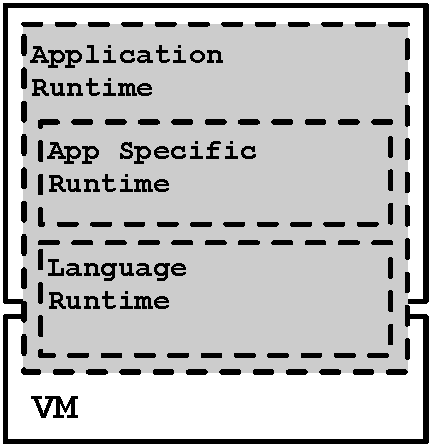
\includegraphics[width=0.5\linewidth]{elements_to_evolve}
\caption{\textbf{Dissection of a running program to evolve.}\label{fig:whatToEvolve} }
\end{center}
\end{figure}

We identify inside a running application the following elements. First, the application runtime contains the \emph{application specific} and the \emph{language} runtimes that represent respectively the elements of the application under execution and the language that provides support for it. The \VM provides as well an execution support for the application runtime. The overlapping shows the interrelations between these three components.

\subsection{Application Runtime}

The application runtime is the set of software elements that constitute an application during its execution. An application runtime includes software elements that describe the application's structure, such as its libraries, classes and methods, and elements related with the application's execution, such as threads, the execution stack with its activation records and created objects. In the context of this thesis, we do not consider the Virtual Machine(\VM) as a part of the application runtime, but as a machine that supports the application runtime.

The subset of the application runtime that describes the language we use is the \emph{language runtime}. The language runtime includes the set of structures and constructs that describe the language concepts and behavior. This language runtime concretizes the model that the language proposes to the developers. For example, Smalltalk and Ruby propose that an application is structured in classes with implicit metaclasses \ie a class is instance of a (\emph{meta})class that describes its behavior. Therefore, they also contain structures that represent the concepts of a \ct{Class} and \ct{Metaclass} and control the implicit creation of a metaclass for each new class. Additionally, a language runtime is not only composed of classes but it also includes objects. For example, it contains a table of unique strings or \emph{symbols} used to univocally name objects. A language runtime is usually common to different applications in the same language: it is always present and contains always the same elements.

Within an application runtime we identify also the \emph{application specific runtime}. The application specific runtime is the subset of the application runtime that includes the elements that belong to the particular application. The application specific runtime follows the model and concepts imposed by the language \ie it is expressed in terms of the language runtime, and thus coupled to it. For example, the application specific classes of a Smalltalk or Ruby application have an implicitly created metaclass.

\subsection{Virtual Machine}

High-level languages virtual machines~(\VMs) provide with support for executing an application runtime.
\VMs concentrate several complex and interconnected elements with two main purposes: first it is to abstract applications from details such as memory management or machine specifics; second it is to do that while also obtaining good performance.
The early \VMs focused on interpreting an abstract instruction set (bytecodes).
On the one hand the bytecodes guarantee certain platform independence by abstracting away from the \CPU specific instruction set.
On the other hand bytecodes allow one to encode complex operations into little space both serving the hard memory constraints of the hardware and simplifying the design of a compiler.
Obviously this abstraction gain comes at a cost, and ever since the first \VMs were built, research and industry strive to reduce the interpretation overhead.

%This goes even so far that specialized hardware is conceived to match the performance requirements \cite{Unga84a,Stef84a,McGh98a,Clic05a}.

To improve performance some \VMs use a just in time compiler (\JIT) that dynamically generates native code from the bytecode \cite{Deut84a}.
In this case the bytecode becomes an intermediate representation (\IR) for a bigger compiler infrastructure.
However, \JIT compilers are notoriously complex as they crosscut many \VM components.
At the same time they crosscut all abstraction layers; they have to access high-level information from the running bytecodes and manage native code at the same time.
Similar complexity applies to the automatic memory management present in most high-level language \VMs.
Garbage Collectors (\GC) evolved from simple helpers to complex software artifacts that for instance support concurrent garbage collection \cite{Clic05a}.

These complex \VMs are the enablers of many of the features in our programming languages. However, their complexity constrain the changes we can apply to our application runtimes. For example, adding a new field into the classes of an application runtime may impact the bytecode interpreter, the JIT, the GC, and so on. These constraints denote the \emph{execution model} of a \VM \ie the contract required to a language runtime to execute it. This execution model includes the format in which the runtime elements are layout in memory~(objects, classes, methods), the followed object model (\eg class-based or prototype-based) and the instruction set that the runtime must implement.

\section{Problem Statement}

This thesis focuses in the generation of specialized object-oriented high-level application and language runtimes. In such context, we identify a main problem: application runtimes usually provide with none or little support to change the structures that represent itself. We lack of an infrastructure for safe application runtime manipulation. This infrastructure must allow both the specialization and extension of application and language runtimes.

Particularly, we identify these more concrete problems that such an infrastructure should solve:
\begin{description}
\item[Unclear \VM-Language interface.] The relation between the language and the \VM, particularly its execution model, remains often unclear in \VM hardcoded assumptions.
\item[Core runtime changes remain low-level.] Changing a language or application runtime representation often forces us to modify the low-level code that defines such a runtime.
\end{description}


\section{Contributions}

The contributions of this thesis are three-fold. The main contribution is \Vtt, an \emph{infrastructure for application runtime virtualization}. This infrastructure allows us to manipulate and control a virtualized application's runtime. \Vtt exposes the \VM-language interface as a first-class runtime object, namely an object space. An object space clarifies and makes explicit such interface, and provides with a high-level API for its manipulation.

We validate our language virtualization infrastructure by exploring two approaches for application runtime manipulation.
\begin{description}
\item[Bootstrapping.] We describe the process to create a language runtime through \emph{bootstrapping} with \Vtt. Our bootstrapping process provides a novel way to define an object-oriented language runtime by using the definition of the language to define itself.
\item[Application tailoring.] We developed a novel dynamic application tailoring approach based on lazy installation, namely Run-Fail-Grow~(RFG). \Vtt supports RFG by allowing the monitoring of the application under extraction and provide with facilities for code installation.
\end{description}

% =============================================================================
\section{Thesis Outline}
% =============================================================================
%\sm{This dissertation structure is different to what I am used to. At least the way you announce the purpose of the chapters is not what I would expect.
%In my diss, everything revolves around one thesis, here, it is a number of things listed one after another, don't see the central motive I would expect}

\gp{write from scratch, left for the end}
\begin{description}
\item[\chapref{background}] 

\item[\chapref{benzo}] 
	
\item[\chapref{ffi}] 

\item[\chapref{validation}] 

\item[\chapref{conclusion}] 

\end{description}


% =============================================================================
\input{chapter-footer.tex}
% =============================================================================

\input{chapter-header.tex}
% ===========================================================================
\chapter{State of the Art}
\chaplabel{background}
\minitoc
% ===========================================================================
\introduction
% ===========================================================================

This chapter presents the related work to this dissertation. With that in mind, we organize and classify the related work in two different axis \ie virtualization aspects and runtime manipulation. The reader would notice that some of the related works we present may fit into more than one of these axis. However, for the sake of clarity, we emphasize the aspects we believe will clarify the understanding of the rest of this thesis.

The first part of this chapter focuses on runtime manipulation of object-oriented applications. We first show related work that focus on the safe modification of language semantics at runtime. Then, we show how metacircular runtimes aim to have an unified language runtime to ease its modification. \gp{I should add some conclusion}

The second part of this chapter starts by presenting a brief introduction to virtualization, its terminology and moreover its usage. We find amongst those usages, that the \emph{co-existence} and \emph{control} of virtual technology may fit into the manipulation of runtimes.
Following, we dive into related work that implement and apply those two techniques, but not in the runtime manipulation scenario as we understand it.\gp{should add some conclusion}

This chapter finishes by presenting a detailed description of the problem statement and a final outlook of the upcoming chapters in the light of the found problems.


% ===========================================================================
\newpage
% ===========================================================================

\section{Modifying the Runtime}
\gp{should really expand this part and say why it is relevant}
Modifying a runtime system can be a cumbersome task. On one side, we recognize that virtual machines and the languages that run on top of then are very interrelated and interdependent software components. For example, a language must comply to the execution model provided by its \VM~(\eg a bytecode set or an object model), and the \VM may understand the language's internals to manipulate it~(\eg run it, optimize it or manage its memory).

On the other side, reflective runtimes have a circular dependency on themselves: they rely on the concept of causal connection\gp{this is actually only true for reflective architectures}. When we make a change in a reflective runtime, we should ensure these causal connections still hold at any point of the runtime's life. In case a causal connection is broken, the runtime may become unusable as there is no means for it to keep reflecting upon itself correctly.

The related work we present in this section presents two main topics of interest for us. First, we present those works that target the modification of a language's semantics by safe means~(\ie avoiding crashes). We follow by looking at the field of metacircular runtimes and \VMs, to study how they ease the modification of a runtime by means of simplifying the language-\VM relation for development.

\subsection{Modification of language semantics}

\subsubsection*{Tower of Interpreters Model}

The original model of reflection as defined by Smith~\cite{Smit82c} is based on meta-level interpretation. A program is interpreted by an interpreter, such interpreter is interpreted by a meta-interpreter and so on, possibly ad-infinitum. This leads to a tower of interpreters, where each floor defines the semantics of the program~(interpreter of application) it interprets~(Figure \ref{fig:tower_of_interpreters}).

\begin{figure}[ht]
\begin{center}
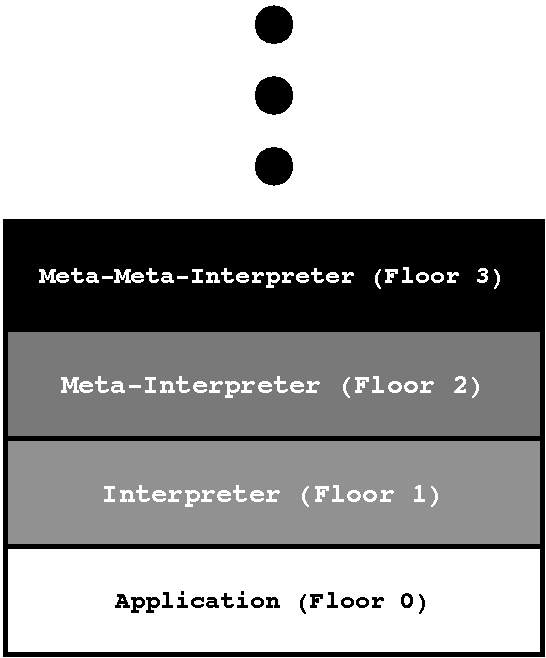
\includegraphics[width=.5\linewidth]{tower_of_interpreters}
\caption{\textbf{The theoretical tower of interpreters model. Each floor interprets the floor below itself.}\label{fig:tower_of_interpreters}
% (a)The host language and (b)the guest language contain each one their own classes and objects. The guest language resides inside the host language during the bootstrap; (c)the builder, a program written in the host language, reifies the bootstrap process itself and bootstraps the guest language given a (d)source code specification.
 }
\end{center}
\end{figure}

The tower of interpreters presents a model where one can define and redefine the semantics of the program it is executing. We can modify the behavior of our program~(in the floor zero) by jumping one level above it in the tower and modifying the interpreter running in that floor. In the same sense, we can jump one level above this interpreter to change also its behavior and so on. This allows the \emph{indirect modification} of a program's behavior \ie a change in an interpreter in a level \emph{n} changes the behavior of the interpreter level \emph{n - 1}, which impacts in the interpreter below it and so on, up to the base level.

Smith's tower of interpreters model is flexible and coherent regarding the manipulation of the reflective behavior of a program. The tower does not present a limit on the amount of interpreters we can stack, presenting a problematic infinite potential. This idea collides with the non-infinite amount resources in current machines. On one side, limited memory prevents us to have a tower of infinite interpreters running at the same time. On the other side, above certain limit of interpreters, this approach becomes too slow and impractical. We will show in the following subsections other reflective models that try to overcome these deficiencies while trying to keep some of the good properties of this model.

\subsubsection*{Black}

Black is a reflective language based on Scheme that mimics the infinite tower of interpreters with the goal to make it practical. Its model is based on the same idea as the reflective tower: the base level is interpreted by an interpreter, which is interpreted by a meta-interpreter and so on. The main difference between the original tower of interpreters and the model presented by Black is that the latter avoids the infinite regression, making the model practical in finite resource machines.

Black avoids the infinite regression by limiting the real levels of interpretation: there is only one level of interpretation. For the rest of the levels, Black  introduces a difference between directly-executed code in contrast with interpreted code. Directly-executed code is code that is executed by the machine, where no interpretation steps are involved. Then, the base-level application is the only interpreted code in the application. The rest of the tower, including the first interpreter, is implemented and executed directly in machine code~(Figure \ref{fig:black_tower}).

\begin{figure}[ht]
\begin{center}
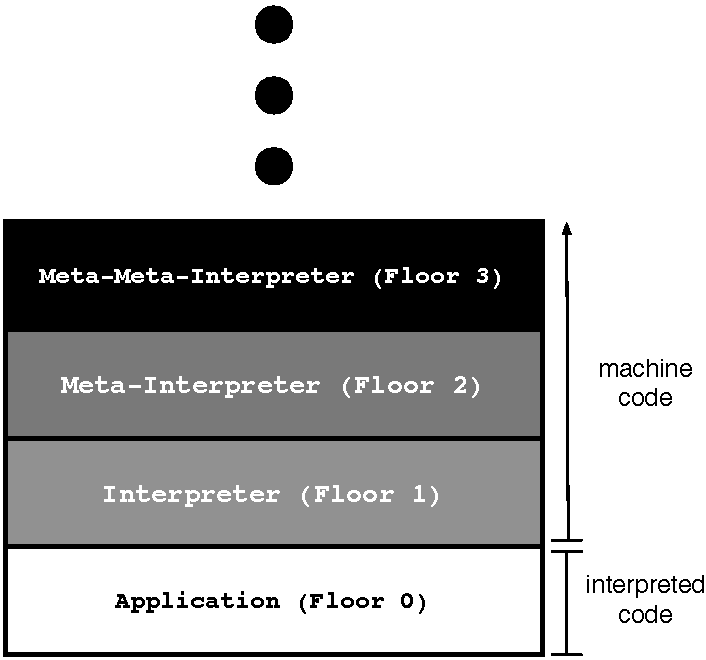
\includegraphics[width=.6\linewidth]{black_tower}
\caption{\textbf{Black.}\label{fig:black_tower}
% (a)The host language and (b)the guest language contain each one their own classes and objects. The guest language resides inside the host language during the bootstrap; (c)the builder, a program written in the host language, reifies the bootstrap process itself and bootstraps the guest language given a (d)source code specification.
 }
\end{center}
\end{figure}

By limiting the levels of interpretation, the model presented by Black forbids \emph{indirect modification}. Changing the interpreter in a level \emph{n} above the first level does not impact any more the interpreters below it, as they are directly-executed in the machine and not by the modified interpreter. Black supports, however, the modification of the first level of interpretation with the introduction of hooks inside the machine code. A hook detects wether a function in the interpreter~(written in directly-executed code) is changed, and interprets it by a meta-level interpreter written also in directly executed code. Hooks degrade the performance in comparison of a non-hooked interpreter, but it allows in exchange to change and specialize the behavior of the directly-executed code.

\subsubsection*{Safe-Tcl}
Safe-Tcl~\cite{Levy97a, Bore94a} is a variation of Tcl whose main purpose is the execution of Tcl scripts in a safe environment, with restricted permissions and attributions. Safe-Tcl achieves this by using \emph{twin interpreters} \ie a normal Tcl interpreter~(the master interpreter) can invoke and configure specialized interpreters that run isolated from the master interpreter~(Figure \ref{fig:safetcl_twin_interpreters}).

\begin{figure}[ht]
\begin{center}
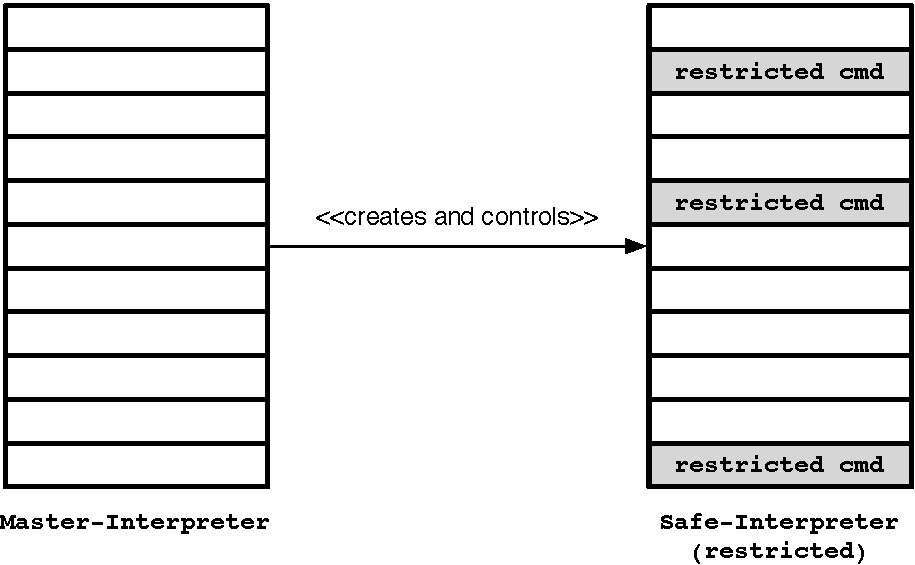
\includegraphics[width=.6\linewidth]{safetcl_twin_interpreters}
\caption{\textbf{Black.}\label{fig:safetcl_twin_interpreters}
% (a)The host language and (b)the guest language contain each one their own classes and objects. The guest language resides inside the host language during the bootstrap; (c)the builder, a program written in the host language, reifies the bootstrap process itself and bootstraps the guest language given a (d)source code specification.
 }
\end{center}
\end{figure}

The master interpreter modifies the behavior of a safe interpreter by providing a security policy. A security policy grants or removes privileges to the scripts executed on an interpreter. Commands can be aliased so the untrusted interpreter call an aliased method and the command is fully implemented by a trusted interpreter.

Safe-Tcl twin interpretation allows us to change the behavior of a program running on a specialized interpreter, without the limitations of the infinite tower of interpreters. However, in contrast with the solutions we already presented, Safe-Tcl does not provide with the ability to change completely the semantics of the language but just to override or provide new commands, with a focus on security.

\subsection*{Reflective Architectures and Reflectivity}

To enable reflection in mainstream languages such as Java, Ruby or JavaScript, the tower of interpreters is replaced by a reflective architecture~\cite{Maes87a}. Instead of relying on a stack of interpreters interpreting each the level below it, a reflective architecture relies on the idea of \emph{causal connection} \ie the programming language incorporates structures that represents aspects of itself~(\eg classes, objects), in such a way that if one structure changes the aspect it represents is updated accordingly, and vice-versa.


In languages presenting reflective architectures, reflection is controlled by a meta-object that lives in the same environment of the object it reflects upon.
One problematic corollary of this is that meta-objects rely on the same code and infrastructure than the objects they reflect upon; therefore there is a risk of infinite meta-recursion when the meta-level instruments code that it relies upon~(Figure \ref{fig:reflectivity_meta_recursion}).

\begin{figure}[ht]
\begin{center}
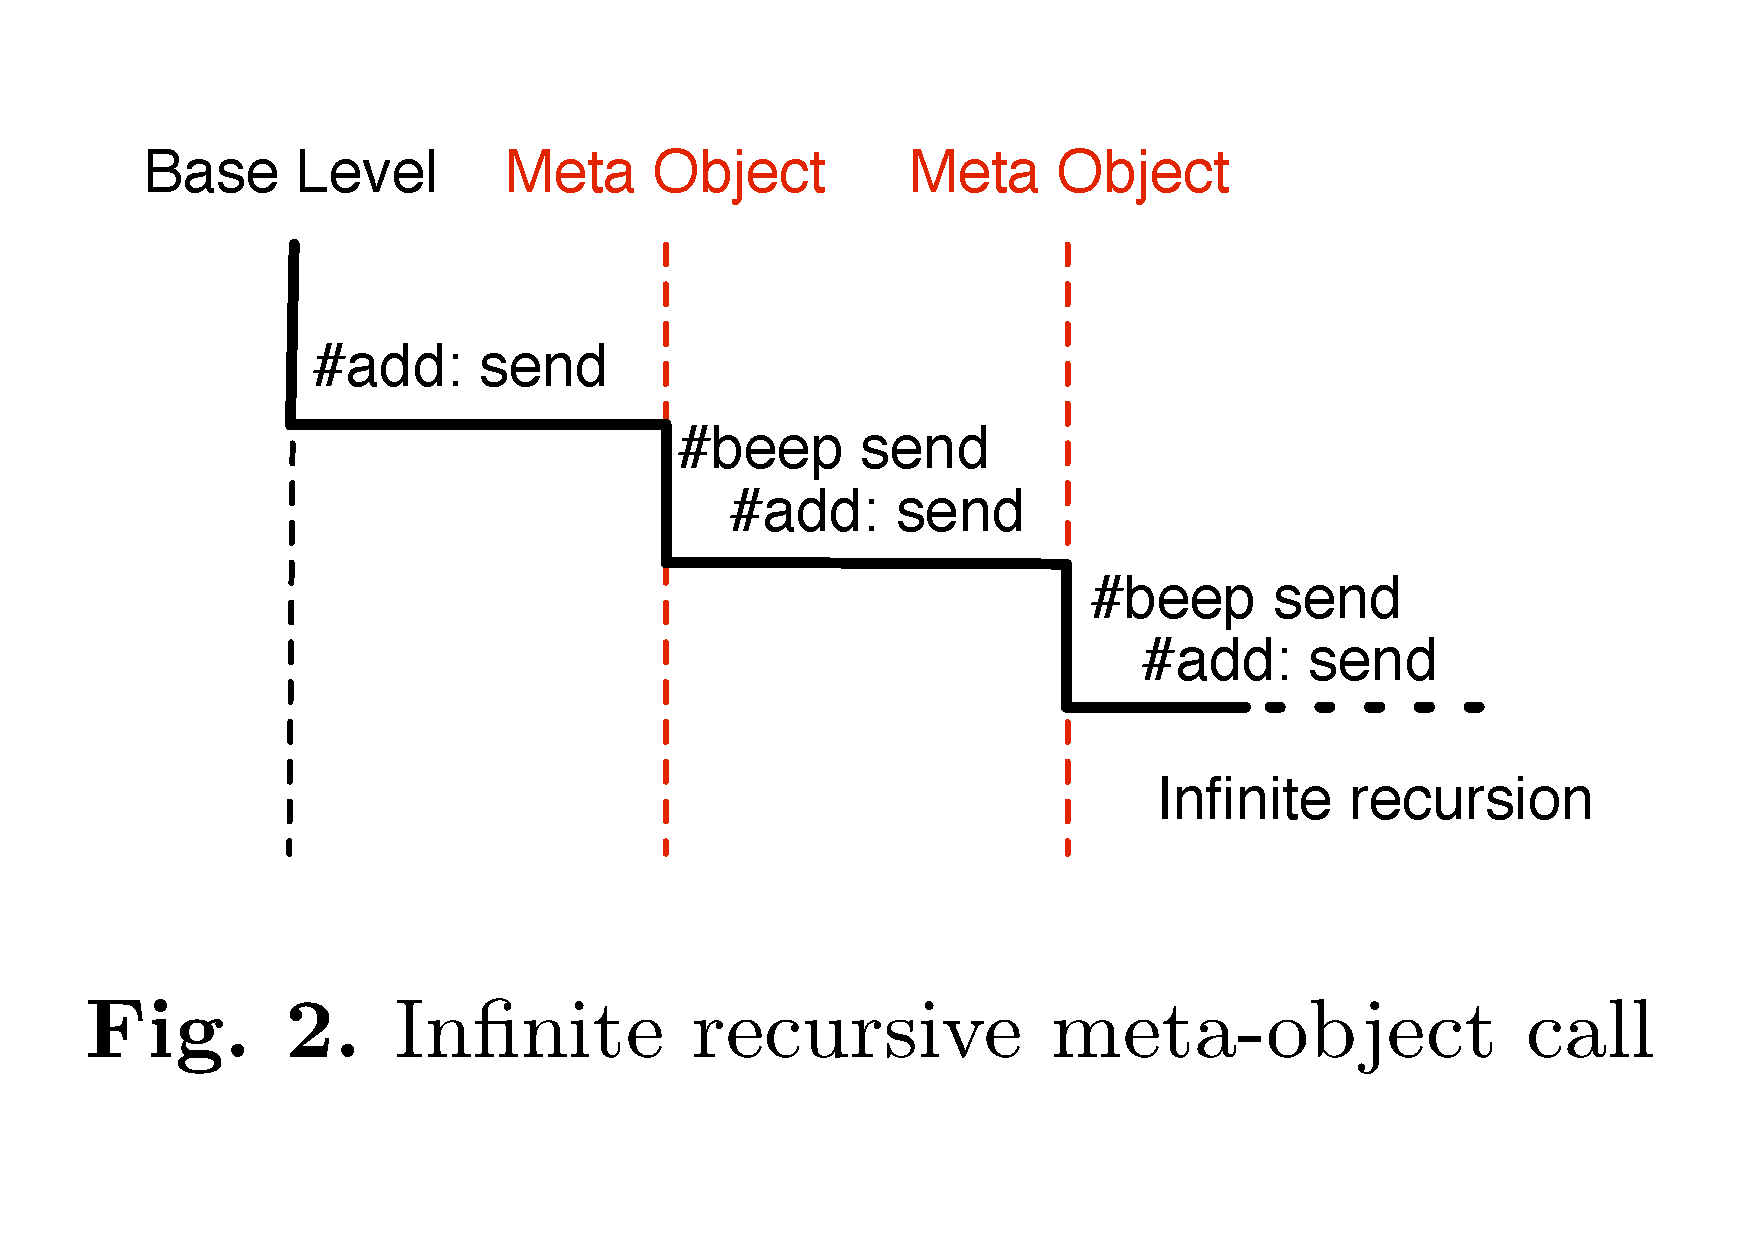
\includegraphics[width=.6\linewidth]{reflectivity_meta_recursion}
\caption{\textbf{Meta level recursion in reflective architectures.}\label{fig:reflectivity_meta_recursion}
% (a)The host language and (b)the guest language contain each one their own classes and objects. The guest language resides inside the host language during the bootstrap; (c)the builder, a program written in the host language, reifies the bootstrap process itself and bootstraps the guest language given a (d)source code specification.
 }
\end{center}
\end{figure}

Denker et al. solve this problem in Reflectivity~\cite{Denk08b}. Reflectivity is a reflective framework that avoids meta-recursions by tracking the degree of metaness of the execution context. In each reflective call, the \ct{MetaContext} object is activated and it accounts the meta-level jump. Likewise, when the reflective call returns, the \ct{MetaContext} is deactivated. Using the accounted meta-level jumps of the \ct{MetaContext}, meta-objects do only reflect on objects of a lower metaness~(and not greater or equal metaness). Thus, it simulates the semantics of an infinite tower of distinct interpreters while there is only one of them~(Figure \ref{fig:reflectivity_meta_recursion}).

\begin{figure}[ht]
\begin{center}
\begin{subfigure}{.45\textwidth}
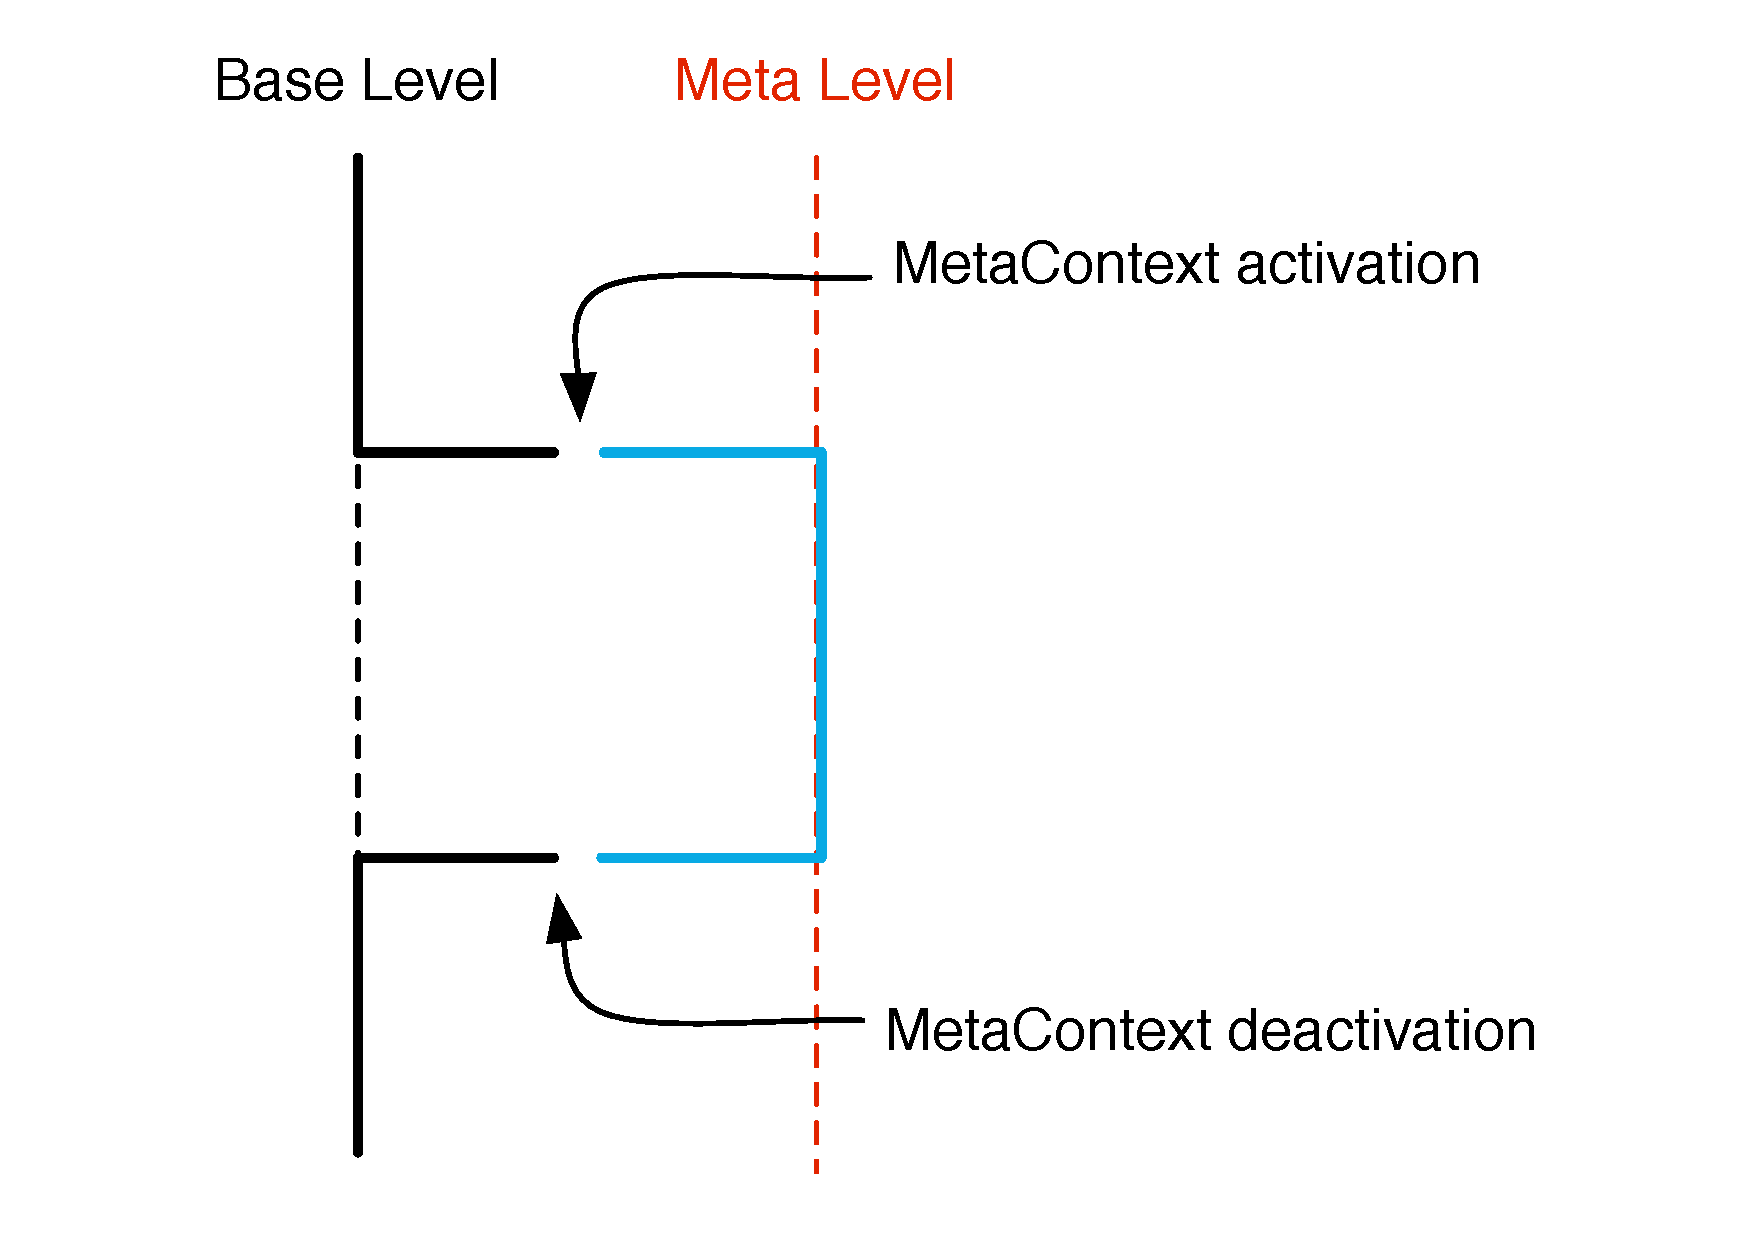
\includegraphics[width=1\linewidth]{reflectivity_metaness_accounting}
\end{subfigure}
\begin{subfigure}{.45\textwidth}
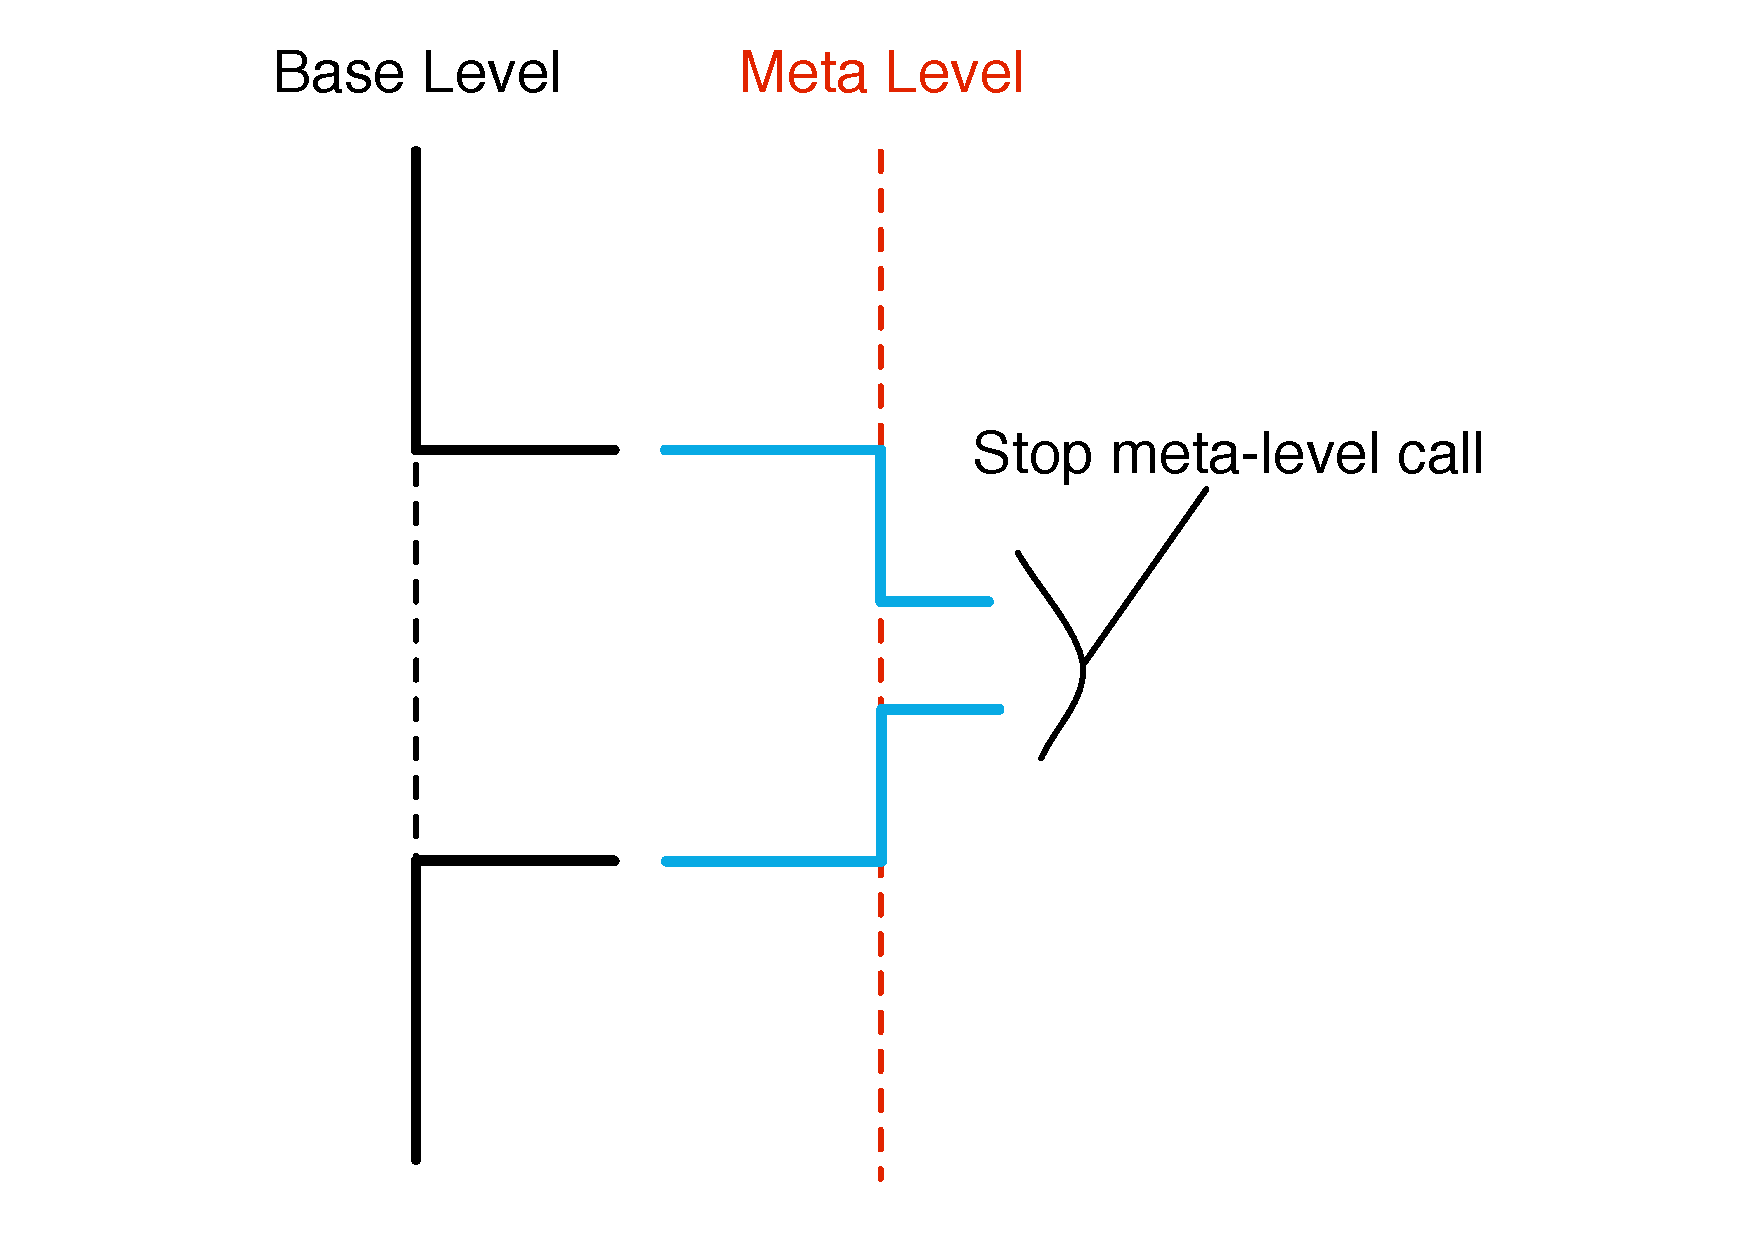
\includegraphics[width=1\linewidth]{reflectivity_avoid_recursion}
\end{subfigure}
\caption{\textbf{Meta level jump using reflectivity.}\label{fig:reflectivity_meta_recursion}
% (a)The host language and (b)the guest language contain each one their own classes and objects. The guest language resides inside the host language during the bootstrap; (c)the builder, a program written in the host language, reifies the bootstrap process itself and bootstraps the guest language given a (d)source code specification.
 }
\end{center}
\end{figure}

Reflectivity succeeds to modify and scope behavioral changes for different meta-levels inside the same reflective architecture. However, it does not provide with support for structural changes of the code the reflective framework depends upon.

\subsection{Metacircular Runtimes}

High-level language \VMs are inherent complex pieces of software.
They have to combine two rather extreme goals: abstraction and performance.
We have seen that the required abstraction for the running high-level language has a strong influence on the \VM design.
At the same time the hard performance requirement requires precise interaction with the underlying hardware.
This goes even so far that specialized hardware is conceived to match the performance requirements~\cite{Unga84a,Stef84a,McGh98a,Clic05a}.

The early \VMs focused on interpreting an abstract instruction set (bytecodes).
The benefits are twofold.
On the one hand the bytecodes guarantee certain platform independence by abstracting away from the \CPU specific instruction set.
On the other hand bytecodes allow to encode complex operations into little space both serving the hard memory constraints of the hardware and simplifying the design of a compiler.
Obviously this abstraction gain comes at a cost and ever since the first \VMs were built research and industry strive to reduce the interpretation overhead.
An efficient way to improve performance is to use a just in time compiler (JIT) that dynamically generates native code from the bytecode~\cite{Deut84a}.
In this case the bytecode becomes an intermediate representation (IR) for a bigger compiler infrastructure.
However, JIT compilers are notoriously complex as they crosscut many \VM components.
At the same time they crosscut all abstraction layers; they have to access high-level information from the running bytecodes and manage native code at the same time.
Similar complexity applies to the automatic memory management present in most high-level language \VMs.
Garbage Collectors (GC) evolved from simple helpers to complex software artifacts that for instance support concurrent garbage collection~\cite{Clic05a}.

The increased complexity of the \VMs lead to more novel approaches on how to build \VMs.
\VMs are still build for a big part in C or C++ for performance reasons.
However, there are more high-level approaches that try to simplify creating \VMs by using building blocks~\cite{Geof10a}.
In the following sections we are shedding light on metacircular \VMs which are programmed in the same language they in the end support.


\subsubsection*{Squeak Smalltalk \VM}
\seclabel{background-squeak}
% ---------------------------------------------------------------------------
The Squeak \VM~\cite{Inga97a} is of importance in the context of this work.
Its core building system is still in active use for the \urlfootnote{Cog \VM}{http://www.mirandabanda.org/cogblog/} which extends Squeak with a JIT compiler.
The Cog \VM is used as default by the \urlfootnote{Pharo}{http://pharo.org/} programming language.
Squeak is built around a Smalltalk dialect called Slang that is exported to C to be compiled to the final \VM binary.
Additionally, the Slang sources can be interpreted to provide an interactive simulator of the \VM, including full graphical support.

Slang is limited to the functionality that can be expressed with standard C code.
Slang in this case is mostly a high-level C preprocessor.
Even though Slang basically has the same syntax as Smalltalk it is semantically constrained to expressions that can be resolved statically at compilation or code generation time and are compatible with C.
Hence Slang's semantics are closer to C's than to Smalltalk's.
Unlike later metacircular frameworks, Squeak uses little or no compile-time reflection to simplify the \VM designs.
However, class composition help structuring the sources.
Next to the Slang source which account for the biggest part of the interpreter code some operating system related code and plugins are written in C.
To facilitate the interaction with the pure C part Slang supports inline C expressions and type annotations.

A great achievement of the Squeak \VM is a simulator environment that enables programmers to interact dynamically with the running \VM sources.
The simulator is capable or running a complete Squeak Smalltalk image including graphical user interface.
This means that programmers can change the sources of the running \VM and see the immediate effects in the simulator.
The simulator itself works by setting up a byte array which servers as native memory.
Then the \VM sources written in Slang are interpreted by the \VM of the development environment.

% ---------------------------------------------------------------------------
\subsubsection*{\Jikes: High-level low-level Programming in with \MMTK}
\seclabel{background-jikes}
% ---------------------------------------------------------------------------
Jikes (former Jalapeño) is an early metacircular research \VM for Java written in Java~\cite{Alpe00a}.
The Jikes \VM features several different garbage collectors and does not execute bytecodes but directly compiles to native code.
With metacircularity in mind Jikes does not resort to a low-level programming language such as C for these typically low-level \VM components.
Instead they are written in Java as well using a high-level low-level programming framework.

The Jikes \VM had performance as a major goal, hence direct unobstructed interaction with the low-level world is necessary using a specialized framework.
High-level low-level programming \cite{Fram09a} is mentioned the first time in the context of the Jikes \VM project.
The goal of high-level low-level programming is to provide high-level abstractions to simplify low-level programming.
Essentially this is the same motivation that drives the metacircular \VM community.

Frampton et al. present a high-level low-level framework packaged as \ttt{org.vmmagic}, which is used as a system interface for Jikes. This package introduces highly controlled low-level interaction in a statically type context.
In their framework, methods have to be annotated to enable the use of low-level functionality.
Additionally their framework is successfully used in a separate project, the memory management toolkit (\textsc{MMTK})~\cite{Blac04a} which is used independently in several other projects.


% ---------------------------------------------------------------------------
\subsubsection*{\Maxine \Java \VM}
\seclabel{background-maxine}
% ---------------------------------------------------------------------------
\Maxine is a metacircular \Java \VM \cite{Wimm13a} focused on an efficient developer experience.
Typically \VM frameworks focus on abstraction at the code-level which should yield simpler code and thus help reducing development efforts.
However, in most situations the programmer is still forced to use existing unspecific tools for instance to debug the \VM.
In contrast to that, the \Maxine \VM provides dedicated tools to interact with the \VM in development.
\Maxine uses abstract and high-level representations of \VM-level concepts and consistently exposes them throughout the development process.
Inspectors at multiple abstraction levels are readily available while debugging, giving insights to the complete \VM state.
\Maxine provides and excellent navigation for generated native code by providing links back to language-side objects as well as other native code and symbols.

Even though the \Maxine projects follows an approach where reflection is only used at compile-time, the development tools themselves provide a live interaction with the running \VM artifact.
However, the \VM itself is not reflective as it is not directly built to reason about itself.
This means that when debugging the \VM it behaves almost like a living \ST image where a complete interaction with the underlying system is possible.
We identify this as crucial, as most of the time is spent debugging, notably on inadequate tools like \ttt{gdb} due to lack of alternatives.
Hence having a specific debuggers and inspectors greatly improve the interaction with the \VM artifact.


\subsubsection*{\PyPy Toolchain}
\seclabel{background-pypy}
% ---------------------------------------------------------------------------
\urlfootnote{\PyPy}{http://pypy.org/} is a \Python-based high-level \VM framework \cite{Rigo06a}.
\PyPy's major focus lies on an efficient \Python interpreter.
However, it has been successfully used to build \VMs for other languages including \ST \cite{Bolz08a}.
Interpreters are written in a type-inferable subset of \Python called \RPython.
The underlying \PyPy infrastructure automatically provides memory management and \JIT compilation.
Instead of explicitly providing these features, a \VM developer hints certain information to the \PyPy framework to improve the generation of a \GC or \JIT.

\PyPy follows a different approach from the previously presented \VM generation frameworks.
For instance, in Squeak and \Jikes the final \VM implementation is not much different from an implementation done directly in a low-level language.
The programmer specifies all the components of the \VM explicitly, either by implementing them directly or using a provided library.
Compared to the more static C ans C++ these \VM generation frameworks make the compilation phase more tangible.
\ST in \Squeak or \Java in \Jikes or \Maxine fulfill the purpose of the template system in C++ or the restricted macro system in C.
For the explicit implementation part \PyPy is no different.
However, certain features for the final \VM are directly absorbed from the underlying \PyPy infrastructure.
For instance, the \JIT support or the \GC are not explicitly implemented but provided by the \PyPy framework itself.
This is a big difference to the other \VM frameworks as it allows programmers to write the \VM in a more high-level fashion.
For instance in \Squeak memory allocation, even for \VM-level objects, has to be performed explicitly.
Whereas in \PyPy the garbage collection is left to the underlying \VM building infrastructure.
This approach allows \RPython \VMs to behave like standard \Python programs.

Much like the automatic memory management, \PyPy provides a tracing \JIT generator \cite{Bolz09a}.
By default the \VM programmer does not write an explicit \JIT in \PyPy.
Instead the \VM code is annotated to guide the underlying tracing \JIT generator.
This means a \VM compilation time a specific tracing \JIT is created for the given meta information.
As a result, the \JIT can track high-level loops in the final interpreted language.
Again, this is similar to \PyPy's \GC, both are provided as a service and do not have to be programmed explicitly.
Instead, the \VM programmer tweaks parameters of the \JIT or \GC.

% ------------------------------------------------------------------------------
\subsubsection*{\Pinocchio \VM}
\seclabel{background-pinocchio}

\P \cite{Verw11a} is a research \ST environment that directly uses native code instead of bytecodes.
The only execution base is native code which is directly generated by the language-side compiler.

\P is built from a kernel derived originally from a \PH image.
For the bootstrap classes, objects and methods are exported into binary, native images and linked together with a standard C linker to a final executable.
For simplicity we also rely on a very small part of C code to provide essential primitive, for instance used for file handling.
Additionally we specified part of the bootstrap for the \ST object model in plain C code.
However, besides that, all the other code is written and developed directly in \ST.

An important aspect of \P is that the method lookup is expressed in terms of normal \ST code.
Typically this code statically resides in the \VM, thus at a different meta-level.
Hence this implies for most systems that the lookup can not be modified without altering the \VM itself.
However, expressing the lookup in terms for normal language-side code introduces a recursive dependencies during the bootstrap.
In order to run the lookup code expressed in \ST code, we have to perform message sends.
These, in return, require an already working lookup mechanism.
Hence, without a taking special care, a language-side lookup method will lead to infinite recursion during startup.
We resolved this problem in \P by directly interacting with the low-level execution format which among other things relies on inline caches to improve performance.
The important property of inline caches is that they bypass the slow language-side lookup by directly jumping to the last activated method at a send-site.
This is exactly the behavior we need to prevent recursion during the startup.
Hence, when generating the native code for the bootstrap, we prefill all the inline caches of the methods required to perform a full method lookup.
As a result, when running requiring the first real method lookup, the lookup code itself is running perfectly on the prefilled inline caches.
What we achieve is a flexible connection between the low-level world and the high-level language-side.
During execution the \VM jumps freely between what previously was native \VM-level code and interpretation of language-side code.

% ------------------------------------------------------------------------------
\subsubsection*{\Klein \VM}
\seclabel{background-klein}

\urlfootnote{\Klein}{http://kleinvm.sourceforge.net/} is a metacircular \VM for the \Self programming language that has no separation into \VM and language \cite{Unga05a}.
It is important to point out that the reification of the \VM-level survives the code generation or compilation time.
Instead the \VM structures are represented as real \Self objects.
Hence the \Klein \VM supports true \VM-level reflection since there is only a single code base.

Additionally to the advances in reflection and metacircularity, \Klein focuses on fast compilation turnarounds to allow for a responsive development process.
Which is unlike for instance the \Squeak \VM where a full \VM bootstrap takes an order of minutes on modern hardware.
\Klein also supports advanced mirror-based debugging tools to inspect and modify a remote \VM.

Development on the \Klein \VM stopped in 2009 and left the \Klein \VM in fairly usable state.
Like \P it currently lacks a dedicated \GC.
Yet, it proved that it is possible and build a language-runtime without the classical separation of the language-side and the \VM.
From the literature presented about the \Klein project we see a strong focus on the improvements of the development tools.
The fact that the language-runtime allows \VM-level reflection to change the \VM dynamically is not directly mentioned in the literature.
While we see the practical limitations of changing the \VM at runtime we would like to open the doors to this new form of reflection.

\section{Virtualization Techniques}

\gp{introduction}

\subsection{Application Co-existence}

\subsubsection*{\textsc{Class Loaders}}
In Java, classes are loaded dynamically through a class loader~\cite{Lian98a}. A class loader is a first-class entity responsible of loading classes: create their runtime representation, loading their methods and linking their class references. A class loader remembers all classes it loaded, and it is responsible for loading all classes related to  them. Class loaders define namespaces: different class loaders can load different classes with the same name. These classes will be isolated in the sense that they will not be visible to the others.

Class loaders can be specialized and extended to provide custom behavior. For example, Fong et. al.~\cite{Fong10a} use the class loading mechanism to enforce scoping rules and determine the visibility of names in various region of the program. They allow the user to control untrusted
namespaces and classes, they have defined a language to define security policy. Jensen et. al.~\cite{Jens98a} provide a formalization of the class loader with the means to enforce security. They also use a bytecode verifier on class loading to check if a class' bytecode doesn't try to perform overflow or underflow operations.

The isolating mechanism of class loaders is useful in the scoping context. New versions of code can be loaded in a different class loader and coexist at runtime. However, its basic mechanism does not support a way to manage changes, or update an application.

\subsubsection*{\textsc{Changeboxes}}

Changeboxes~\cite{Denk07c} is a change model designed to encapsulate and scope changes. Its main purpose is to allow several versions of a system to coexist at runtime \ie the existence in the same environment of different versions of the same classes and methods. In changeboxes, a \emph{changebox} is a first-class entity that encapsulates changes made on elements~(classes and methods) and an executable version of the system with its changes applied. The system can contain many changeboxes at the same time, and applications can be scoped to run within different changeboxes. This notion of dynamically scoping an application to a changebox allows one to have co-existing environments~(\eg testing, development, production), increasing the developer's efficiency. Furthermore, it eases application update and migration to new versions, and reduces its update down-time as the application does not have to be stopped to be updated.

A Changeboxes prototype was developed in Smalltalk and its scoping mechanisms were implemented as follows:

\begin{description}
\item[Message send interception.] Message sends can activate different methods, within different changeboxes. A MethodWrapper~\cite{Bran98a} is placed instead of the method that has multiple versions, and it delegates the execution to the method that corresponds to the currently valid changebox.

\item[Class access interception.] Smalltalk resolves class names at compile time, inserting a reference to the given class inside the method's literal array. However, accessing a class should yield different class objects if the changebox contains a different version of it. To resolve this, class accesses affected by a changebox are postponed until runtime, and the code is recompiled in such a way: instead of putting the class inside the literal array, the class is dynamically looked-up from the class table when it is accessed.
\end{description}

Changeboxes model proves sound to update and migrate application and framework classes. However, it has the main drawback of not affecting critical classes in the system. Changeboxes prototype does not work on classes such as \ct{Array} or \ct{CompiledMethod} as the underlying infrastructure~(the VM) restricts the system to the existence of only one of them at the same time. The changes model does not provide neither a solution for this problem, as it focuses on application code update, leaving this as an open problem.

\subsubsection*{\textsc{Caja\textbackslash Cajita}}

\subsubsection*{\textsc{Worlds}}
Worlds~\cite{Wart08a} provide a way to control and scope side-effects in Javascript. Side-effects are limited to a first-class environment.

\subsubsection*{\textsc{Gemstone}}
Gemstone \cite{Otis91a} provides the concept of class versions. Classes are
automatically versioned, but existing instances keep the class (shape and
behavior) of the original definition. Instances can be migrated at any time.
Gemstone provides (database) transaction semantics, thus state can be rolled
back should the migration fail.
Gemstone's class versions extend the usual Smalltalk class evolution mechanism for robustness, 
large datasets, and domain-specific migration policies. In contrast, ObjectSpaces target general 
reflective access and bootstrap-like evolutions of code that is critical to the environment.

\subsubsection*{KaffeOS}
KaffeOS \cite{Back00a} makes an explicit domain separation in memory by using different memory heaps in the virtual machine. They enforce domain separation by using memory write barriers. Cross-domain references become cross-heap references, and thus, they need special virtual machine support.
KaffeOS presents a model where resource accounting is handled at the level of the virtual machine.

\subsubsection*{J-Kernel}
J-Kernel \cite{Hawb98a}

\subsubsection*{Luna}
 and Luna \cite{Hawb02a} present a solution similar to ours regarding the memory usage. They are Java solution for isolating object graphs with security purposes. In them, each object graph is called a \emph{protection domain}. All protection domains loaded in a system, and their objects, share the same memory space. 

The J-Kernel enforces the separation between domains by using the Java type system, the inability of the Java language to forge object references, and by providing capability objects\cite{Levy84a,Mill03a,Spoo00a} enabling remote messaging and controlling the communication. This same separation in Luna \cite{Hawb02a} is achieved by the modification of the type system and the addition in the virtual machine of the \emph{remote reference} concept.

\subsection{Application Control}

\subsubsection*{JVMTI}
Java also provides JPDA, a remote debugging architecture that specifies a native interface on the debuggee VM, and a matching API for the debugger front-end, running in a separate VM. However, JDPA only supports introspection features like  inspection and monitoring, and very limited intercession \cite{jdpa}.

\subsection*{Xen and Operating System Virtualization techniques}
Amongst the most important works on virtualization,we can found approaches like Xen~\cite{Chis07xen}. Xen is a Virtual Machine Monitor~(VMM) that allows to control and manage Virtual Machines in a high performance and resource-managed way. This approach targets the virtualization of full and unmodified operating systems, to facilitate their adoption in industrial/productive environments. Virtualization, in these terms, enables the following applications:

\begin{description}

\item[Server Consolidation.]
\item[Co-located hosting facilities.]
\item[Distributed web services.]
\item[Secure computing platforms.]
\item[Application Mobility.]

\end{description}

This virtualization approach has another main characteristic: it considers its guest systems as a black box, and it does not allow one to observe or modify its internals.

\subsubsection*{MVM: a Multi User Virtual Machine}
The Multi-user Virtual Machine~\cite{Czaj03a,Czaj01a} is a general purpose virtual machine for the Java language that allows the co-existence of different applications, potentially from different users. Each application running on top of the MVM is an \emph{isolate} based on the Java Application Isolation API specification~\cite{JSR121}.

Many isolates co-exist not inteferring each other, as they believe they own their private JVM: the runtime is modified, so state is not shared between them by default. MVM allows several communication mechanisms to securely communicate isolates: from standard mechanisms such as sockets, up to \emph{links}, a low-level isolate-to-isolate mechanism introduced by the Isolate API.

MVM can run any normal Java application. Additionally, MVM-aware applications can use the API it provides to control the life-cycle~(\eg creation, suspension, resuming and and termination) and the available resources of other isolates.

%\subsection*{Java Isolates}
%Java Isolates \cite{JSR121} allow multiple applications to run inside the same Java virtual machine.
%Nothing is shared between the different applications. Resources like CPU time, memory are controlled 
%and restricted. Isolates can communicate through channel, since nothing is shared the data are copied. 
%Java Isolates are defined in the Java Specification Request 121, but no commercials Java virtual 
%machine implement the specification.

\section{Problem Statement}

% =============================================================================
\input{chapter-footer.tex}

\part{\VTT: an Application Runtime Virtualization Infrastructure}
\input{chapter-header.tex}

% ===========================================================================
\chapter{\VTT: Virtualized Application Runtimes}
\chaplabel{vtt}
\minitoc
% ===========================================================================
\introduction
% ===========================================================================

This chapter presents the model of our Virtualization Application Runtime infrastructure, namely \VTT~(cf. Section \ref{sec:virtualization_overview}). In \VTT, an application runtime is virtualized by residing inside a controlled space, namely an \emph{object space}, that encapsulates the access to it. A first-class representation of this object space provides a high-level API to easily query and manipulate the application runtime~(cf. Section \ref{sec:object_space}). The client of an object space is a \emph{runtime hypervisor}~(cf. Section\ref{sec:hypervisor}).

\begin{figure}[htb]
\begin{center}
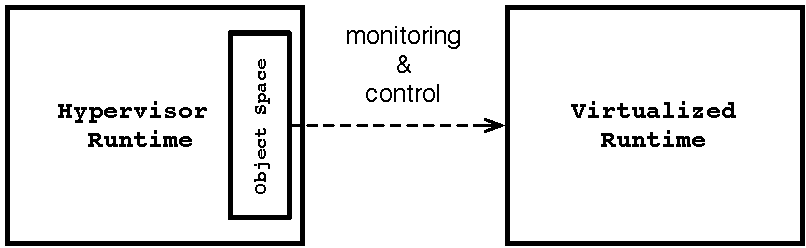
\includegraphics[width=.7\linewidth]{virtualization_introduction}
\caption{\textbf{Virtualization concepts in \Vtt.}\label{fig:virtualization_introduction}}
\end{center}
\end{figure}

The runtime hypervisor runs in the same process than the virtualized runtime to monitor and manipulate it directly. However, the runtime hypervisor does not share the same application runtime than the virtualized runtime it supervises \ie basic objects, classes and \VM structures are not shared between the runtime hypervisor and the virtualized runtime. Instead, both the virtualized and hypervisor runtimes contain their own copies of those elements. This no sharing strategy pursues to allow the hypervisor to change any part of the virtualized runtime without affecting itself as it happens in reflective architectures~(cf. Figure \ref{fig:virtualization_introduction}).

A first class runtime hypervisor manipulates the virtualized runtime through a first-class object space object. This hypervisor can also perform cross-runtime message-sends by injecting processes, as the direct message-send \VM mechanism would fail the method lookup~(Section \ref{sec:isolation}).
Finally, a more granular control can be made through virtual execution. For this, a virtual code interpreter provides full intercession power over the execution of the virtualized application for usages such as tracing or debugging~(Section \ref{sec:interpretation}).

This chapter focuses on the model of our solution and presents its core ideas. The following \chapref{prototype} will present the particular implementation details of our prototype implementation of \Vtt on Pharo.

%On one side, this means that the hypervisor can freely manipulate the virtualized language runtime without affecting itself. On the other side, this no-sharing strategy poses an extra effort in communication~(cf. Section \emph{sec:isolation}) mainly in object marshaling.

%A language hypervisor is a first-class object in \VTT, meaning that we can easily modify it and replace it by another object. Additionally, a simulation mode allows a fully-managed execution mode.

%We do not require any changes in existing applications to import them inside an object space. We introduce minimal modifications at the \VM level to ensure their control and manipulation is transparent. Regarding execution, an object space provides with different means for controlling the execution of the language runtime it owns~(cf. Section \ref{sec:execution}). It can safely start, pause and resume its execution, create new threads or finalize existing ones.  


\section{\Vtt Architecture} \label{sec:virtualization_overview}

\Vtt presents an architecture where multiple application runtimes can co-exist on the same process independently from each other. They do not share any \VM or language state \ie each one has its own interpreter, stack, classes and objects. In this setting, a virtualized application runtime is an application runtime that is monitored by another application runtime. The application runtime that takes the role of controlling the virtualized runtime is the hypervisor runtime. The hypervisor runtime is a full-fledged application runtime, providing us with the expression power and abstractions of a high-level language to express our runtime hypervisor. A first-class object space object represents the virtualized runtime and provides operations for its manipulation. A first-class runtime hypervisor object uses the object space and implements a particular manipulation on it \eg runtime update, failure detection, browsing and debugging. Figure \ref{fig:objectSpaceOverview_architecture} provides an overview of the \Vtt's architecture.

\begin{figure}[htb]
\begin{center}
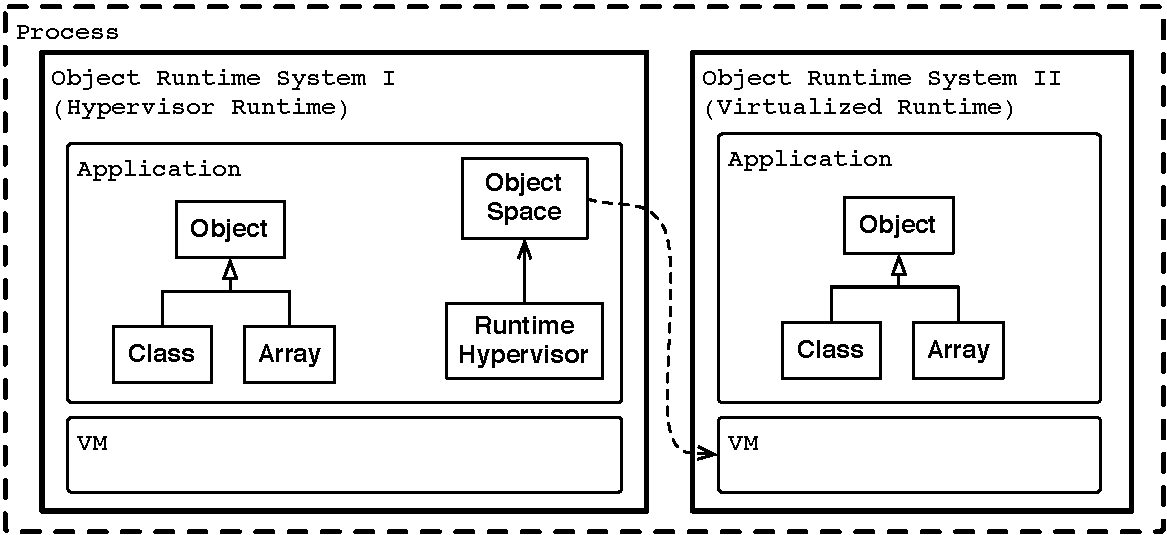
\includegraphics[width=1\linewidth]{object_space_overview3}
\caption{\textbf{\VTT Overview.} A runtime hypervisor in the runtime I (left) manipulates the runtime II (right) through an object space.\label{fig:objectSpaceOverview_architecture}}
\end{center}
\end{figure}

An object space manipulates the virtualized runtime directly, changing the target's application runtime state and manipulating the \VM-language interface. All modifications are applied from the outside of the target virtualized runtime, in contrast with reflective architectures where such changes are applied from the same application runtime under modification. Doing so provides \Vtt with the following properties:

\begin{description}
\item[Transparency.] Our solution does not require any changes in the applications residing inside the virtualized runtime. Thus, we can virtualize existing application runtimes without modifying them \ie \Vtt does not require virtualized applications to include particular libraries, use particular interfaces nor change their execution model.

\item[Application independence.] Our solution does not depend on the particular application inside the virtualized runtime. Different runtime hypervisors can be written for different use cases, including application specific and general ones. The limitation of this approach is, however, its dependance on the execution model imposed by the \VM.
\end{description}

\section{Object Spaces: First-class Application Runtimes} \label{sec:object_space}

An object space is a first-class representation of an object oriented application runtime, meant for its manipulation and control. An object space encapsulates an application runtime and provides with a clear and explicit interface to manipulate it. This interface is split in two different kind of objects: an \ct{objectSpace} object provides general operations on the virtualized runtime while mirror objects~\cite{Brac04b} provide operations to manipulate individual objects that reside inside it~(Figure \ref{fig:objectSpaceMirrors}). Specific mirrors, such as the \ct{ClassMirror}, manipulate elements with a different object-format or runtime representation to enforce their internal representation.

\begin{figure}[htb]
\begin{center}
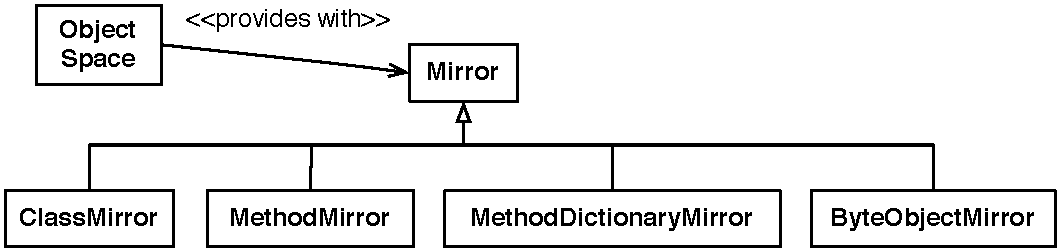
\includegraphics[width=.9\linewidth]{object_space_mirrors}
\caption{\textbf{Mirrors in Object Spaces.} An object space is the main entry point for runtime manipulation. An object space provides with mirrors to modify particular runtime elements. \label{fig:objectSpaceMirrors}}
\end{center}
\end{figure}

These objects make explicit through the operations they expose two important parts of a \VM-language interface, explained in detail in the following subsections. First, The \VM setup interface exposes the elements of the language that should be initialized so it can run a program. Second, the runtime manipulation interface exposes operations that take part at runtime to manipulate runtime structures such as objects, classes, threads, the execution stack.

\subsection{\VM Setup Interface}

The \VM setup is the configuration the \VM needs to run.
For example, a \VM may need the boolean objects \ct{true} and \ct{false} to push them as the result of a boolean operation at runtime.
This configuration is usually done only during the language runtime initialization, before execution of a program, as the \VM cannot easily anticipate the usage of such elements in a program from beforehand.
The \VM setup interface allows us to configure the following kind of elements:

\begin{description}
\item[Well-known objects of the language.] Objects such as \ct{nil}, \ct{true} or \ct{false} are needed at runtime for different purposes. For example, the garbage collection needs \ct{nil} at runtime to update weak references. Other particular objects may be held by the \VM as prototypes to speed-up instantiation time of commonly used objects.

\begin{code}
ObjectSpace {
    mirror getNil();
    mirror getTrue();
    mirror getFalse();

    void setNil(mirror aNilObject);
    void setTrue(mirror aTrueObject);
    void setFalse(mirror aFalseObject);
}
\end{code}

\item[Special classes.] Special classes are those needed by the \VM at runtime. They are needed to perform safety checks, create instances or handle special cases such as immediate objects. For example, when mutating a \ct{String} object the Pharo \VM checks that the introduced object is a \ct{Character} object, to avoid putting the \ct{String} into an invalid state. Also, the \VM requires references to those classes that it instantiates directly~(instead of being created through the \ct{new} message in program). For example, the Pharo \VM instantiates a \ct{BlockClosure} object when it founds the bytecodes that correspond a block expression at runtime. Finally, immediate objects are objects that are encoded inside an object reference instead of occupying a place inside the heap. Immediate objects do not include a reference to their class and therefore the \VM needs to know how to map each particular reference encoding to its corresponding class to perform the method-lookup. 

\begin{code}
ObjectSpace {
    void setArrayClass(classMirror anArrayClass);
    void setBlockClass(classMirror aBlockClass);
}
\end{code}

\item[Special messages.] Special messages are callbacks that the \VM will invoke into the application to notify particular events. The probably most known of such messages is Smalltalk's \ct{doesNotUnderstand}~(the equivalent to \eg Ruby's \ct{methodMissing}). When the \VM does not find a method matching a message-send, it will send a \ct{doesNotUnderstand} message to the receiver object and let the user program decide what to do in such a case.

\begin{code}
ObjectSpace {
    void setDoesNotUnderstandSelector(mirror aSelector);
}
\end{code}

\end{description}

This \VM setup interface avoids to hardcode particular knowledge of a language inside the \VM. This gives us the possibility to easily change particular language internals such as renaming special messages or changing the class hierarchy of special classes without leaving the runtime in an inconsistent state. Being radical, we could think on porting another language to this VM, as long as they share similar execution semantics \ie the \VM execution model is compatible with the given language and we configure this interface accordingly.


%In our particular implementation the list of classes exposed through this interface are those of literal objects and those related with the internal \VM execution model. For the sake of completeness the list of classes is the following: \ct{Array}, \ct{Association}, \ct{BlockClosure}, \ct{ByteArray}, \ct{ByteString}, \ct{ByteSymbol}, \ct{Character}, \ct{Context}, \ct{Float}, \ct{SmallInteger}, \ct{LargePositiveInteger}, \ct{LargeNegativeInteger}, \ct{Message}, \ct{CompiledMethod}, \ct{MethodDictionary}, \ct{Semaphore}, \ct{WeakFinalizationList}.

\subsection{Runtime Manipulation Interface} 
The runtime manipulation interface includes operations to monitor and modify the application runtime during execution. This interface provides access to the application runtime internal elements and encapsulate the implementation details behind them~(\ie the object-format imposed by the \VM). This interface provides the following kind of operations:

\begin{description}
\item[Runtime Global Access.] An object space offers operations to query and modify the global state of the runtime. For example, it provides access to the loaded classes or the running threads/processes. It exposes as well operations to install new and remove existing ones.

\begin{code}
ObjectSpace {
    "Classes"
    mirror createClass(String name, int formatOfInstances);
    List<mirror> getClasses();
    mirror getClass(String name);
    void removeClass(String name);
    ...

    "Threads"
    List<mirror> getThreads();
    List<mirror> instalThread(threadMirror thread);
    ...
}
\end{code}

\item[Runtime Object Access.] Mirrors~\cite{Brac04b} expose the operations to query or alter a particular object or element in the runtime. Different kind of mirrors enforce the object-format of the different type of objects we can manipulate. For example, we expose specific mirrors for normal objects, classes, methods, activation records or processes. Notice that these mirrors are low-level mirrors as they expose operations to mutate and access objects in their \VM representation. Additionally, through mirrors we can execute \VM primitives on objects, providing the correct primitive ID~(an integer or native function pointer, depending on the implementation) and the corresponding arguments. These primitives are operations that the \VM exposes normally to the language.

\begin{code}
Mirror {
    "Class access"
    classMirror getClass();
    void setClass(classMirror aClass);

    "Field Access"
    mirror getInstVar(String varName);
    void setInstVar(String varName, mirror anObject);
    
    "Primitive execution"
    mirror executePrimitive(primitiveID id, mirror receiver, Array args);
}
\end{code}

\begin{code}
ClassMirror {
    "Instantiation"
    mirror instantiate();
    mirror instantiate(int aSize);

    "Method manipulation"    
    void compileMethod(String sourceCode);
    void removeMethod(String selector);
}
\end{code}

\end{description}

% ===========================================================================

\section{First-Class Runtime Hypervisors}\label{sec:hypervisor}

The client of an object space is a \emph{runtime hypervisor}. A runtime hypervisor is first-class entity that implements a particular monitoring/modification strategy. A runtime hypervisor monitors an object space by splitting the execution in cycles. These cycles are delimited by a time window and finished in safe suspension points~(Figure \ref{fig:execution_cycle})\ie a safe suspension point is a moment in execution where suspending a thread will not leave it in an inconsistent state. For example, in our \Vtt prototype written for the Pharo language, safe suspension points are the activation of message sends and bytecode backjumps. During each execution cycle, the virtualized runtime runs unmanaged using the full \VM's capacity. When the cycle finishes because the execution completed a time window and found a suspension point, the control is returned to the runtime hypervisor. Then, the runtime hypervisor applies its corresponding action and resumes the execution of the virtualized runtime from the last suspension point.

\begin{figure}[ht]
\center
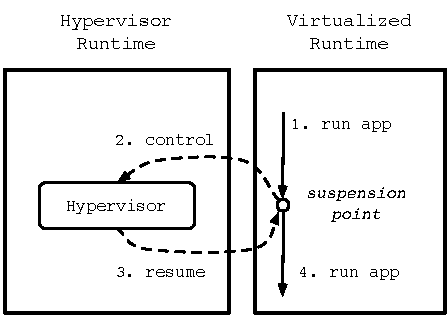
\includegraphics[width=.6\linewidth]{execution_cycle}
\caption{\textbf{Execution Cycle.} \label{fig:execution_cycle}}
\end{figure}

To allow cycle execution, we extended the \ct{objectSpace} interface to execute during a cycle of time. An \Vtt implementation should additionally include support for suspension points. This operation will awake the virtualized runtime processes and execute them for a time window. Once the time window is finished, it will be suspended in the next suspension point and the control will return to the runtime hypervisor.

\begin{code}
ObjectSpace {
    void runCycle();
}
\end{code}

%Our implementation presents an execution cycle of 200ms that allows us to have fine grained control while the virtualized application has still place to run. We use as suspension points backjumps found in the executed bytecode and message sends. In such a way, we ensure that the execution stack is in a consistent state after it is interrupted.

Then, our runtime hypervisor class hierarchy presents four basic methods. First, the \ct{run} template method implements the basics of the hypervision cycle: it resumes the execution of the virtualized runtime inside a loop. Two methods~(\ct{before} and \ct{after}) provide hooks for the specific hypervisor implementations. Figure \ref{fig:hypervisors} shows a class hierarchy example and code with two sketched runtime hypervisors. A \ct{NullHypervisor} allows the virtualized runtime to run without any intervention. The \ct{UpdateHypervisor} instead checks the existence of a file with updates on every cycle.

\begin{code}
Hypervisor >> run
    [ true ] whileTrue: [
        self before.
        self basicRun.
        self after.
    ]

Hypervisor >> basicRun
    objectSpace runCycle.

NullHypervisor >> before
    "Nothing"

NullHypervisor >> after
    "Nothing"

UpdateHypervisor >> before
    self checkForUpdate.

UpdateHypervisor >> checkForUpdate
    "We check if a given file exists"
    'update.txt' asFile exists ifTrue: [ ...
    ...
\end{code}

\begin{figure}[ht]
\center
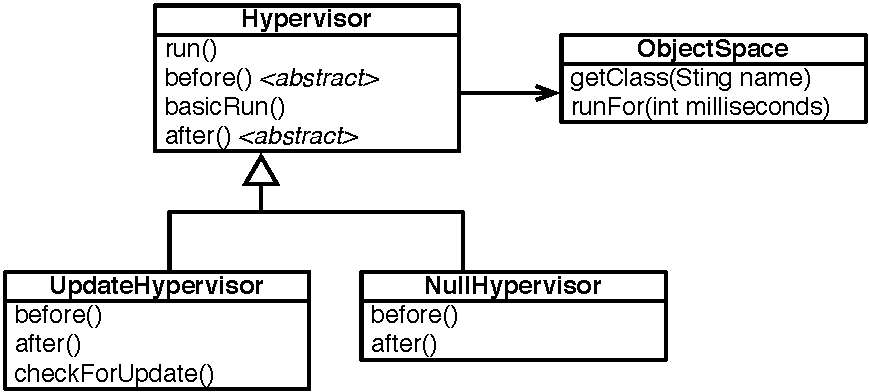
\includegraphics[width=.9\linewidth]{hypervisors}
\caption{\textbf{Example Runtime Hypervisors Class Hierarchy.} A \ct{NullHypervisor} does nothing while the \ct{UpdateHypervisor checks for updates before every cycle execution}.\label{fig:hypervisors}}
\end{figure}

\section{Cross-Runtime Communication} \label{sec:communication}\label{sec:isolation}

A runtime hypervisor may require to apply some operation in a virtualized runtime that would be more difficult through direct object manipulation with mirrors. Let's take as an example a virtualized application that uses a particular logging library. In the context of that application, disabling logging would mean to execute the following statement:

\begin{code}
Logger disable.
\end{code}

And the code invoked should be:

\begin{code}
Logger class>>disable
	self uniqueInstance disable
	
Logger>>disable
	enabled := false
\end{code}

However, doing the same through our abstract layer of mirrors presents the following drawbacks (a) to replicate the behavior of the \ct{disable} method inside the hypervisor and (b) to couple it to the internals of such a logging library. 

\begin{code}
OurHypervisor>>disableLogging
	logger := objectSpace getClass: #Logger.

	"the logger is a singleton"
	"in a class variable named uniqueInstance"
	loggerInstance := logger classVariablesAt: #UniqueInstance.

	"The enabled instance variable is the first"
	loggerInstange instanceVariableAt: 1 put: false.
\end{code}

Thus, a runtime hypervisor may benefit from the execution of an arbitrary expression or statement within the scope of the virtualized runtime. For example, enabling or disabling a logger from the virtualized application can be easily achieved through executing the following statement in the runtime hypervisor instead of manually modifying the state of the logger objects:

\begin{code}
objectSpace execute: [ Logger disable ].
\end{code}

To achieve this kind of communication, we observe the following challenges in using a plain \VM's message-send mechanism with our no sharing strategy.

\begin{description}

\item[Cross-Runtime Method-Lookup.]A \emph{cross-runtime message-send}~(from the hypervisor to the virtualized runtimes) cannot be simply achieved by the usual message-send mechanism. The usual message-send mechanism looks up in the receiver's class hierarchy a method with an \emph{object identical} method signature. However, our not-sharing strategy prevents the normal method-lookup work on a \emph{cross-runtime message-send} as symbols and classes are not shared between the different runtimes. In such a case, the method-lookup mechanism fails because the elements of a message signature and the method signature we target are indeed \emph{equals but not identical}~(Figure \ref{fig:cross_runtime_lookup}).

\begin{figure}[ht]
\center
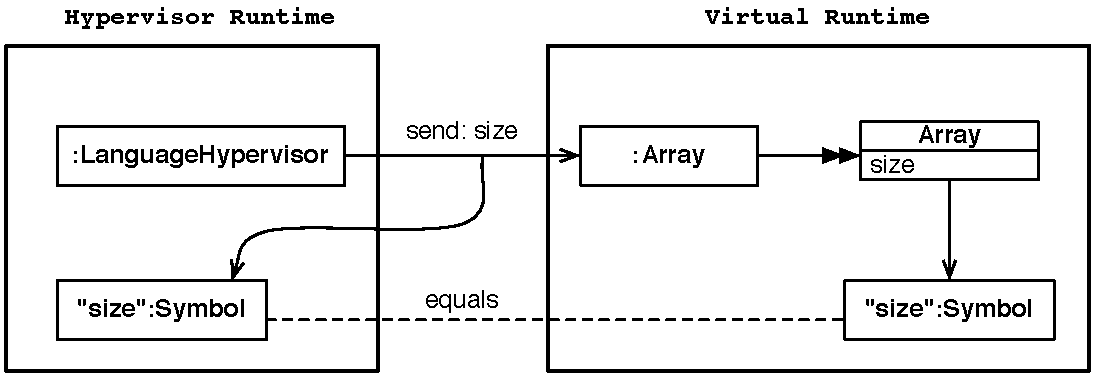
\includegraphics[width=.9\linewidth]{cross_runtime_lookup}
\caption{\textbf{Failing Cross-Runtime Method Lookup.} The runtime hypervisor sends the \ct{size} message to an array in the virtualized runtime. This message-send signature is the hypervisor runtime's \ct{size} symbol. The \ct{size} method exists but its signature has a different \ct{size} symbol. Both symbols are equals but not identical, and thus the lookup fails.\label{fig:cross_runtime_lookup}}
\end{figure}

\item[Exceptions and Stack.] A cross-runtime method-lookup succeeds if we modify the runtime hypervisor message-send to contain the right symbol from the virtualized runtime. In such case, the execution stack contains a mixture of activations that belong to the hypervisor and virtualized runtimes. This poses a problem under the presence of techniques that traverse the execution stack indiscriminately, such as the exceptions or stack manipulation techniques such as Smalltalk's \ct{thisContext} special variable. The presence of such elements may leak object references from a runtime to another, leaving them in inconsistent state~(Figure \ref{fig:mixed_stack}) \gp{cite some paper like j kernel on exceptions leaking references}.

\begin{figure}[ht]
\center
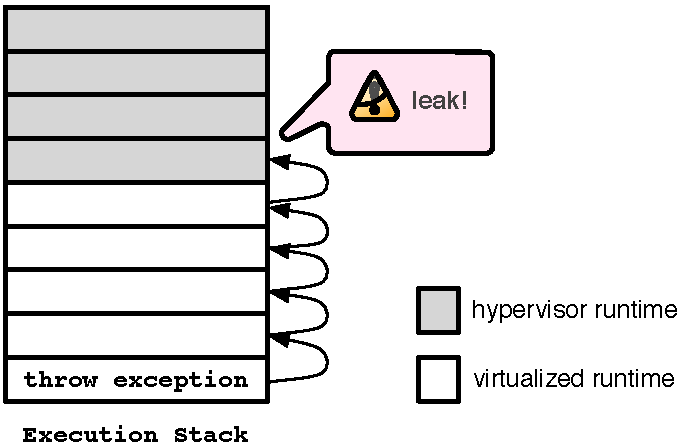
\includegraphics[width=.6\linewidth]{mixed_stack}
\caption{\textbf{Reference Leaks in a Mixed Stack on Exception.} When mixing the execution stack between the virtualized and hypervisor runtimes, an exception may traverse the stack and have access to a reference from a different runtime.\label{fig:mixed_stack}}
\end{figure}

\end{description}

To overcome these problems we base the cross-runtime communication on \emph{process injection}. We create a new process/thread inside the virtualized runtime containing the expression to execute. The new process is installed in the virtualized runtime and executed in cycles until it is finished. Once finished we can access the result of the expression through a mirror. The objects that conform the message-send signature and other literals~(\eg strings, numbers) are translated from their representation in the hypervisor runtime to their corresponding representation in the virtualized runtime. Global object references such as classes are mapped to their corresponding references in the virtualized runtime. Non-global non-literal objects can be specified explicitly as an argument:

\begin{code}
objectSpace
	execute: [ :aLogger | aLogger disable ]
	with: aLoggerInstanceMirror.
\end{code}

This solution for cross-runtime communication solves both problems observed before. In a first place, it prevents the method-lookup failure by translating the objects part of the method signature. Second, the new process executes in its own stack ensuring none of the objects from the hypervisor are leaked to the virtualized runtime.

\section{Virtual Execution through Interpretation} \label{sec:interpretation}

\Vtt allows a \emph{virtual execution} mode through interpretation. Virtual execution takes place by doing code interpretation of either abstract syntax trees~(ASTs) or bytecode. In \Vtt a virtual code interpreter is a first-class entity that interprets code inside a virtualized runtime and has full control on the interpreted code. The virtual interpreter is useful in cases where the virtualized runtime is in an incoherent or buggy state and it cannot execute code by itself. In those cases, the virtual interpreter can be used to fix the problem in the virtualized runtime before it can continue its own execution. For example, we can use the virtual code interpreter to replace a broken method in the basic class hierarchy:

\begin{code}
"newMethod is a method that fixes the bug"
interpreter := VirtualCodeInterpreter newOn: anObjectSpace.
interpreter
	execute: 'Object methodDictionary at: #brokenSelector put: newMethod'
	with: newMethod.
\end{code}

The virtual code interpreter has three main points of communication with an object space:

\begin{description}
\item[Instance Variable Access.] Accessing or writing an object's instance variable is mapped by the code interpreter to a field access or write in the mirror representing the receiver object.

\begin{code}
VirtualCodeInterpreter >> readInstanceVariableNumber: index
    ^ self receiver instanceVariableAtIndex: index
    
VirtualCodeInterpreter >> writeInstanceVariableNumber: index with: aMirror
    ^ self receiver instanceVariableAtIndex: index put: aMirror
\end{code}

\item[Method Lookup.] On a message-send, the virtual code interpreter performs the method lookup by inspecting the class hierarchy of the receiver object. The receiver object state is exposed to the interpreter by a mirror. Following, we illustrate this with a simplified method lookup:

\begin{code}
VirtualCodeInterpreter >> lookupSelector: selector
    | classToLookup |
    "classToLookup is a class mirror"
    classToLookup := self receiver getClass.
    [ classToLookup isNotNil ] whileTrue: [
        (self class: classToLookup hasSelector: selector)
        	    ifTrue: [ ^ classToLookup ].
	classToLookup := classToLookup superclass.
    ]
\end{code}

\item[Primitive Execution.] In the leaves of the execution, message-sends invoke the language primitives. These language primitives are executed through the object space interface.

\begin{code}
VirtualCodeInterpreter >> invokePrimitiveMethod: aMethod
    ^ self objectSpace
         executePrimitive: aMethod primitive
         receiver: self receiver
         arguments: self arguments
\end{code}

\end{description}

Being a first-class entity, we can specialize the code interpreter to instrument code execution in order to override normal behavior or trace the execution. We can for example trace all instance variable writes by overwriting one of the methods above.

\begin{code}
TracingCodeInterpreter >> writeInstanceVariableNumber: index with: aMirror
    | result |
    result := super writeInstanceVariableNumber: index with: aMirror.
    !\emph{self logWriteIn: self receiver atIndex: index with: aMirror.}!
    ^ result
\end{code}

% =============================================================================
\section{Conclusion and Summary}

\Vtt presents an architecture where several application runtimes can share the same process. A virtualized application runtime is subject of monitoring and manipulation from another application runtime, namely the hypervisor runtime. The hypervisor runtime contains a first class representation of the virtualized runtime, an object space. The object space exposes a clear interface to safely access and modify an application runtime. This interface includes operations to configure the virtualized application runtime and operations to modify particular objects from it. The latter is encapsulated in mirror objects.

The execution of the virtualized runtime is organized in cycles. In between cycles, a first-class runtime hypervisor can perform an operation and then resume the virtualized runtime's execution. We ensure that the state of the virtualized runtime keeps its coherence by only suspending it in safe suspension points.

Besides the direct manipulation through mirrors, a runtime hypervisor can perform cross-runtime message-sends for a richer communication using process injection. Process injection prevents failures in the method lookup and avoids stack traversing techniques such as exception to leak cross-runtime references. Additionally, a virtual code interpreter allows us to execute code on the virtualized runtime with full intercession. A virtual code interpreter is a first class entity, allowing us to easily specialize and change it.

In following chapters we will show how this infrastructure supports the evolution of a programming application runtime in two different scenarios. First, the recreation of a application runtime using an explicit bootstrap process. Second, an application tailoring technique that specializes an application runtime to contain only elements that are used during runtime.

\input{chapter-footer.tex}
\input{chapter-header.tex}
% ===========================================================================
\chapter{Implementation Details of \Vtt}
\minitoc
% ===========================================================================
\introduction
% ===========================================================================

We implemented \Vtt on the Pharo platform. Our solution virtualizes Pharo runtimes and provides, as already described, the ability to manipulate their object graph and control their execution. Our implementation includes a language side library containing the object space and language hypervisor related classes. Our main modification to Pharo's runtime is an extension to its stack-based \VM. This \VM is a version of Pharo's \VM without a Just In Time~(JIT) compiler. This extensions are meant to allow the co-existence of many runtime systems on the same \VM and to allow us to easily modify the \VM setup interface.

An object space VM-Setup Interface in \Vtt~(Section \ref{sec:setup_interface}) is implemented by exposing the \VM interpreter state. The Pharo \VM interpreter state is hold inside an array, so called \emph{special objects array}, which contains references to the objects that the \VM may need at runtime. We expose and modify this array through an object space. The special objects array also provides support for the execution of several runtimes on top of the same \VM. In our solution, the \VM has a single bytecode interpreter shared amongst the different running runtimes. To allow the execution of a different runtime, we exchange the interpreter state for the state of its corresponding runtime in an atomic operation that we call \emph{context switch}~(Section \ref{sec:context_switch}).

\Vtt mirror implementation~(Section \ref{sec:implementation_mirrors}) does not require particular changes in the Pharo \VM. We base our mirror implementation in two existing \VM primitive operations that allows us to execute a primitive on an arbitrary object by changing the primitive's receiver. Additionally, the already existent reifications of objects such as \ct{CompiledMethod}, \ct{Process}~(threads) or \ct{Context}~(stack frames or activation records), allows us to manage such runtime elements using the same mirror mechanism and avoid specific solutions.

\Vtt's presents a memory layout where the objects of both the virtualized and hypervisor co-exist in the same heap~(Section \ref{sec:memory}). This means that there is no need for special support on \emph{cross-runtime references} for implementing \eg mirrors, and that we can reuse the existing memory management in the virtual machine almost transparently.
However, this solution forbids us to analyze the memory usage of the virtualized runtime and has an impact on the GC.

Finally, This chapter finishes, with means of completion, by presenting the non-implemented aspects of our solution~(Section \ref{sec:not_yet_implemented}).

\section{\VM-Setup Interface}\label{sec:setup_interface}

Pharo \VM holds the state of the \VM-setup interface inside a \emph{special objects array} object. Pharo's special objects array contains 56 entries whose indexes are well known by the \VM for their access at runtime. To implement our \VM-setup interface, we access and modify this special object array. Following, we detail the special objects array entries that we expose for our solution.

\begin{description}
\item[Special Instances.] Special instances such as \ct{nil}, \ct{true} and \ct{false} are directly pushed by the \VM interpreter at runtime instead of residing in a method literal list. A flyweight \ct{Character} table contains the first 256 character objects to ensure their identity and save memory.

\item[System Dictionary.] The system dictionary contains all installed classes in the system. An object space uses this entry to query the installed classes and to install new ones. The \VM does not make any special use of this object as it is managed directly from the language.

\item[Process Scheduler.] The process scheduler contains all existing processes~(threads) in the runtime. We can install and remove process from the process scheduler. The \VM uses this same process scheduler to manage the runtime's execution.

\item[Symbol Table.] The symbol table gathers is the set of \emph{unique} strings in the system. Symbols are mainly used to denote method signatures and ensure reference equality during the method lookup. An object space uses the symbol table to map symbols between runtimes and so it ensures no duplicate symbols are created. The \VM does not make any special use of this object as it is managed directly from the language.

\item[Literal Classes.] Literal classes are the classes of literal objects. Literal objects are those present directly in a method's literal list~(\eg numbers, strings, literal arrays), or those objects that the \VM creates at runtime~(\eg BlockClosures). On one side, the \VM uses the classes available in this list to directly instantiate objects of these types or perform safety checks at runtime~(which cannot be performed at compile time because of reflection or the dynamically-typed nature of the language). On the other side, an object space uses these well-known classes to perform transformations between objects in one runtime to another \eg translate a string from the hypervisor runtime to a string in the virtualized runtime.

\item[Special Selectors.] The special selectors denote those messages that the \VM will send to the image under special situations. This is the case of the \ct{doesNotUnderstand} selector that is sent to the receiver object when the method lookup fails finding a method under a message-send. Other selectors in this category are (a)\ct{cannotInterpret} which is sent when a class in the middle of the method lookup has no method dictionary, (b) \ct{mustBeBoolean} which is sent when a branch operation founds a non-boolean object, (c) \ct{cannotReturn} and \ct{aboutToReturn} are selectors used when contexts are finalized and (d)\ct{run:with:in:} is the message used to implement method wrappers.

\end{description}



%Particularly, the special objects array contains a process scheduler object and its corresponding process objects, implementing green threads. Pharo virtual machine has a single threaded nature and uses green threads to organize its execution.

\section{Cycle Execution and Context Switch} \label{sec:context_switch}

The Pharo \VM has single threaded execution. Only one operating system thread is used to execute Pharo code, so process scheduling is handled internally by the virtual machine. Processes scheduled using this approach are also called \emph{green threads}. Green threads provide process scheduling without native operative system support while limiting the proper usage of modern multicore CPUs. By using green threads only one process, the \emph{active process}, is executed at each instant in time. After the active process executes for a given window of time, if there are any waiting processes with greater or equal priority, the active process gets preempted \ie it is suspended and the process with the highest priority becomes the new active process.

In \Vtt, we reused part of the green thread mechanism to schedule runtime execution, which we called \emph{context switch}. A virtualized language runtime runs for a window of time after which it gets preempted if another runtime with highest priority~(the language hypervisor runtime) is waiting. Internally, the \VM has a single bytecode interpreter shared amongst the different running runtimes. To perform the context switch, we exchange the special objects array of the \VM interpreter by the one in the language runtime to resume, and then resume the \VM execution. This solution keeps the single threaded nature of the \VM meaning that when a language runtime is running the others are suspended. On the good side, there are no concurrency problems between the different language runtimes, allowing us to focus on the language specialization features.


\begin{figure*}[htb]
\begin{center}
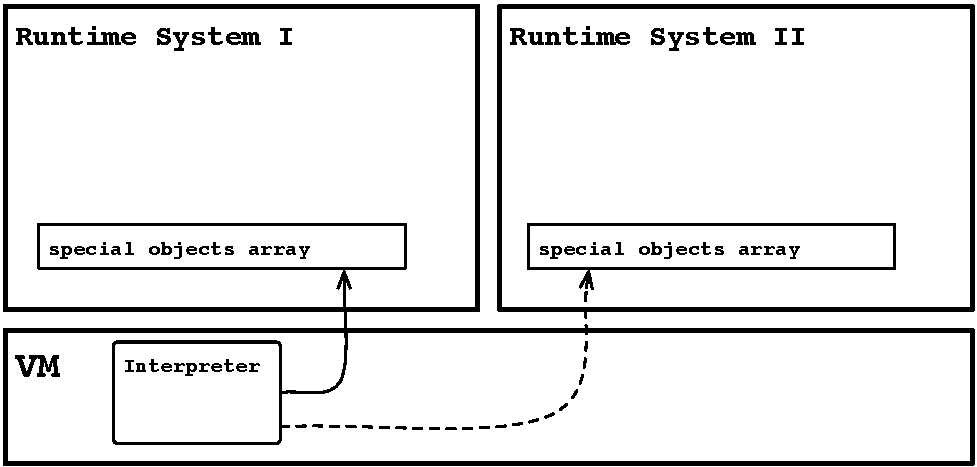
\includegraphics[width=.8\linewidth]{object_space_context_switch}
\caption{\textbf{Context Switch Internals.}To perform a context switch, we change the special objects array of the \VM's interpreter.\label{fig:context_switch}}
\end{center}
\end{figure*}

Finally, the window time control was implemented reusing the existing process preemption mechanism in the \VM. A separate thread, namely the \emph{heartbeat}, is awaken every 200 milliseconds and activating a flag that indicates a preemption can occur. When the \VM code interpreter arrives to one of the safe suspension points (\ie a point where suspending the current execution will not leave the current process in a incoherent state) such as a back jump or a message-send bytecode, the code interpreter preempts the active process if the corresponding flag was activated. In \Vtt we modified the preemption code to activate another language runtime if available.

\section{Mirror Implementation}\label{sec:implementation_mirrors}

Our implementation of mirrors manipulate the objects inside an object space by using already Pharo \VM primitives. A primitive in Pharo is a function executed at the \VM level. To execute a primitive from the language, this primitive should be available as a method. Then, we have to send the corresponding message to the a object subject of the primitive:

\begin{code}
Array >> size [
    <primitive: 62>
]

{1 . 2 . 3} size.
\end{code}

We want however, to avoid cross-runtime message-sends~(\chapref{vtt}), we bypass the message-send with the combination of two existing primitives:
\begin{description}
	\item \textbf{Execute a given method on an object.} Given a method, it is possible to execute it on an object, avoiding method lookup in the object. In current Pharo \VM, this primitive is implemented in the method \textbf{\ct{receiver:withArguments:executeMethod:}} of the \ct{CompiledMethod} class, with number 188. This method receives as arguments the object on which the primitive will be executed, an array of arguments, and the methods to execute.
	\item \textbf{Execute a primitive on an object.} It is possible to send a message to an object, so a primitive is executed on the receiver. This primitive is implemented in Pharo's \ct{ProtoObject} class as \textbf{\ct{tryPrimitive:withArgs:}} with number 118 and receives as argument the number of the primitive and an array or arguments.
\end{description}

We use primitive \ct{receiver:withArguments:executeMethod:} to execute the primitive method \ct{tryPrimitive:withArgs:} on the object from the guest image, avoiding the \emph{cross image-message send} and executing directly the primitive on the given object.

\begin{code}
CompiledMethod
       receiver: anObjectFromOtherRuntime
       withArguments: { aPrimitiveNumber . anArrayOfArguments }
       executeMethod: (ProtoObject >> #tryPrimitive:withArgs:)
\end{code}

We have one mirror per type of object supported by the Pharo \VM. Notice that as some runtime elements such as methods, activation records or even processes are reified as objects in Pharo, we can manipulate them through mirrors without developing new support for them in the \VM:

\begin{description}
\item[Object mirrors.] Mirrors for objects containing just object references such as an \ct{Array} or an \ct{OrderedCollection}.
\item[Word mirrors.] Mirrors for objects containing only non-reference word fields such as a \ct{Float} or a \ct{WordArray} object.
\item[Byte mirrors.] Mirrors for objects containing non-reference byte size fields such as a \ct{ByteArray} or a \ct{ByteString}. 
\item[Class mirror.] Mirrors for class like objects. They control the manipulation of classes and honor the format of a class in the Pharo \VM which should necessary have as its first three instance variables the superclass of the class, its format and method dictionary.
\item[Method dictionary mirror.] Mirrors for method dictionaries honoring the \VM invariants for method installation \ie using the identity hash of the key object instead for doing the lookup in the method dictionary.
\item[Method mirror.] Mirrors for method objects. Method objects in the Pharo \VM are objects with a mixed format. They contain object references to their literals, and byte fields with their bytecode.
\item[Context mirror.] Mirror for context objects. A context object is reified lazily by the Pharo \VM and contains a variable amount of fields denoting the local variables of a scope.
\item[Process mirror.] Mirror for process objects. Process objects are used to manage the execution of a Pharo runtime. They can be resumed, suspended or finalized.
\end{description}


%Using Oz, we can also create and install new processes inside an \objectspace given a code expression. The creation of a process requires the creation of a compiled method with the code~(bytecode) corresponding to the desired expression and a method context. The compiled method with the code to run is obtained by compiling the expression in the host and creating an \objectspace compiled method. The \objectspace compiled method is then provided with the compiled bytecode and its corresponding literals.

\section{Memory Layout} \label{sec:memory}

In \Vtt, all objects belonging to the different language runtimes share a unique object heap. Objects are mixed in this heap and are objects from the same language runtime not necessarily contiguous, as shown in Figure \ref{fig:heap}. Although they are mixed, they are logically separated as they conform different object graphs. Pharo being a safe-language~\cite{Hawb98a,Hawb02a} prevents us to forge references~(\ie creating references from numbers using pointer arithmetic) and isolates the object graphs of each runtime system.

\begin{figure}[ht]
\begin{center}
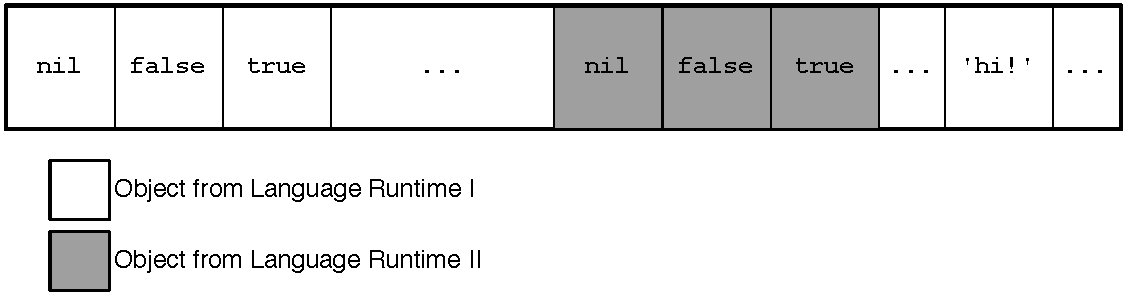
\includegraphics[width=.9\linewidth]{object_spaces_heap}
\caption{\textbf{A unique heap containing objects from different language runtimes.} Objects from the language runtime I and language runtime II are mixed in the heap. In this figure, after the \ct{nil}, \ct{true} and \ct{false} instances that belong to language runtime I, follow the corresponding ones of the language runtime II, which can in order be followed by objects of the former, like the string \textbf{`hi'}. \label{fig:heap}}
\end{center}
\end{figure}

This decision is funded on minimizing the changes made to the virtual machine, because of its complex state of the art. Our decision, while easing the development of our solution, has the following impact on it:

\begin{description}
	\item[Reuse memory handling mechanisms.] We use the same existing memory infrastructure as when \Vtt is not used. Existing mechanisms for allocating objects or growing the object memory when a limit is reached can be reused transparently by our implementation. 
	\item[Simplify the object reference mechanism.] References from mirror objects are normal object references. No extra support from the virtual machine was developed in this regard.
	\item[Shared garbage collection.] Since objects from the different runtimes are mixed in the object memory, and their boundaries are not clear from the memory point of view, the garbage collector~(GC) is shared between them. Every GC run must iterate over all their objects, increasing its time to run.
\end{description}

%This solution seems suitable  J-Kernel \cite{Hawb98a} and Luna \cite{Hawb02a} present a solution similar to ours regarding the memory usage. They are Java solution for isolating object graphs with security purposes. In them, each object graph is called a \emph{protection domain}. All protection domains loaded in a system, and their objects, share the same memory space. 

%The J-Kernel enforces the separation between domains by using the Java type system, the inability of the Java language to forge object references, and by providing capability objects\cite{Levy84a,Mill03a,Spoo00a} enabling remote messaging and controlling the communication. This same separation in Luna \cite{Hawb02a} is achieved by the modification of the type system and the addition in the virtual machine of the \emph{remote reference} concept. In our solution, the separation is given by the same inability to forge object references and the membrane objects that control the communication.

%\section{Creating an \objectspace} \label{sec:object_space_creation}
%
%An \objectspace can be created either from scratch or by loading an existing image. Loading an existing image was implemented as a virtual machine primitive, because the image snapshot is actually a memory snapshot and therefore, easier to handle at VM level. This primitive, implemented with the code shown in Figure~\ref{code:import_image}, reads the snapshot file, puts all objects into the object memory, updates the object references to make them coherent and finally returns the special objects array of the loaded image.
%
%\begin{figure}[htb]
%\begin{code}
%\textbf{primitiveLoadImage}
%    | headerlength bytesRead newImageStart rootOffset oldBaseAddress dataSize rootOop fileObject |
%    
%    "get the reference to the file object"
%    fileObject := self stackValue: 0.
%
%    "Where will we put the new objects"
%    newImageStart := objectMemory startOfFreeSpace.
%
%    "read image header"
%    self readLongFrom: fileObject.
%    headerlength := self readLongFrom: fileObject.
%    dataSize := self readLongFrom: fileObject.
%    oldBaseAddress := self readLongFrom: fileObject.
%    rootOffset :=
%          (self readLongFrom: fileObject) - oldBaseAddress.
%    
%    "seek into the file the start of the objects"
%    self seek: headerlength onFile: fileObject.
%    
%    "grow the heap in the ammount of the image size"
%    objectMemory growObjectMemory: dataSize.
%    
%    "read the file into the free part of the memory"
%    bytesRead := self
%                    fromFile: fileObject
%                    Read: dataSize
%                    Into: newImageStart.
%
%    "tell the vm the free space is now after the loaded objects"
%    objectMemory advanceFreeSpace: dataSize.
%         
%    "update the pointers of the loaded objects"
%    self
%          updatePointersForObjectsPreviouslyIn: oldBaseAddress
%          from: newImageStart
%          until: newImageStart + dataSize.
%    
%    "return the special objects array"
%    rootOop := newImageStart + rootOffset.
%    self pop: 2 thenPush: rootOop.
%\end{code}
%\caption{Implementation of primitive \textbf{\ct{primitiveLoadImage}} that loads an image snapshot into the object memory written in Slang
%\label{code:import_image}}
%\end{figure}
%
%On the other side, creating an \objectspace from scratch can be implemented as a bootstrap of the system, following the process defined in \cite{Poli12a}. The \objectspace provides the \textbf{\ct{createObjectWithFormat:}} method to create an object respecting the given format but with an anonymous class, so we can consider it as a "classless" object. This method is used in the first stage of the bootstrap process, when no classes are available in the \objectspace image yet, to create the \ct{nil} instance~(cf. Figure~\ref{code:bootstrap_nil}) and the first classes~(cf. Figure~\ref{code:bootstrap_classes}). Later, when the classes are available, those objects are set their corresponding ones by using the \textbf{\ct{setClass:}} message.

\section{Benchmarks}

To verify the feasibility of this model, we built our \Vtt prototype in the Pharo language. Our prototype includes the \Vtt class libraries and modification on the JIT-less version of the Pharo \VM.
We benchmarked the virtualized execution of our prototype implementation using a subset of the computer language benchmarks game\footnote{\url{http://benchmarksgame.alioth.debian.org/}}.

We executed each of these benchmarks ten times in two different setups. Results are found in Table \ref{tb:benchmarks}. We first benchmarked the Vanilla JIT-less Pharo \VM without any of our changes, to make it a fair base of comparison with our JIT-less solution. Following, we benchmarked our solution using a null hypervisor that performs no action. This case is meant to measure the execution cycle overhead.

%We executed each of these benchmarks in four different setups. Results are found in Table \ref{tb:benchmarks}. We first benchmarked the Vanilla JIT-less Pharo \VM without any of our changes, to make it a fair base of comparison. Afterwards, we benchmarked our solution in three different setups:

%\begin{description}
%\item[Null Hypervisor.] A hypervisor performing no action. This case is meant to measure the cycle overhead. 
%\item[File Checking Hypervisor.] A hypervisor that checks the existence of a File at each cycle. This case is meant to measure an action that does not include an interaction with the 
%\item[Stack Checking Hypervisor.] A hypervisor checking the execution stack of the virtualized runtime on each monitoring cycle. This benchmark forces in our prototype implementation a reification of the execution contexts~(stack frames) and the creation of several mirror objects.
%\end{description}

%\begin{landscape}
 \begin{table}[ht]

 	\centering
 	\begin{tabular}{|l|c|c|}%c|c|}
			\hline
			\textbf{Benchmark}
 			& \textbf{Vanilla Pharo \VM (1x)}
			& \textbf{Null Hypervisor}\\
%			& \textbf{File Checking}
%			& \textbf{Stack Checking}\\
			
% 			\\& \textbf{}
%			& \textbf{}\\
%			& \textbf{Hypervisor}
%			& \textbf{Hypervisor}\\
		\hline
		RegexDNA & 5711ms +/-22 & 5878ms +/-18 \\\hline% & 6142ms +/-11 & 6555ms +/-424 \\\hline
		KNucleotide & 94.00ms +/-0.85 & 100.1ms +/-3.4\\\hline% & 105.8ms +/-3.2 & 134.4ms +/-3.7 \\\hline
		SpectralNorm & 79.8ms +/-1.4 & 86.6ms +/-1.4\\\hline% & 92.7ms +/-6.0 & 110.7ms +/-1.7 \\\hline
		BinaryTrees & 36.80ms +/-0.65 & 37.10ms +/-0.83 \\\hline%& 35.30ms +/-0.66 & 65.20ms +/-0.93 \\\hline
		Mandelbrot & 422.3ms +/-1.4 & 488.0ms +/-6.5 \\\hline%& 494.9ms +/-3.4 & 632ms +/-23 \\\hline
		ReverseComplement & 5.40ms +/-0.48 & 6.80ms +/-0.24 \\\hline%& 6.80ms +/-0.59 & 8.00ms +/-0.60 \\\hline
		ThreadRing & 2.50ms +/-0.41 & 2.50ms +/-0.56\\\hline% & 2.70ms +/-0.90 & 3.20ms +/-0.80 \\\hline
		PiDigits & 0.90ms +/-0.69 & 0.70ms +/-0.66 \\\hline%& 0.70ms +/-0.66 & 0.90ms +/-0.69 \\\hline
		Meteor & 2260.2ms +/-2.6 & 2398.2ms +/-8.5 \\\hline%& 2479ms +/-16 & 3677ms +/-267 \\\hline
		NBody & 21.10ms +/-0.57 & 21.70ms +/-0.66 \\\hline%& 22.6ms +/-1.4 & 37.7ms +/-1.5 \\\hline
%		FannkuchRedux & 0.00ms +/-0.00 & 0.00ms +/-0.00 & 0.20ms +/-0.36 & 0.00ms +/-0.00 \\\hline
		Fasta & 4.30ms +/-0.54 & 5.20ms +/-0.65 \\\hline%& 5.70ms +/-0.61 & 9.30ms +/-0.39 \\\hline
 	\end{tabular}
	\vspace*{0.2cm}
 	\caption{\small\textbf{Language Virtualization Overhead.} Comparing the cycle overhead from a non virtualized Pharo VM to a virtualized one.\label{tb:benchmarks}}
 \end{table}
%\end{landscape}

These results show that our prototype implementation poses an overhead between 0-9\% for the majority of these benchmarks. Special cases are Mandelbrot~(16\% overhead), ReverseComplement~(26\% overhead) and Fasta~(20\% overhead).
There is however room for improvements due to the absence of a JIT compiler, shared garbage collection and the single threaded nature of the system.
\gp{not sure what else put in here, since I cannot exactly explain why the overhead is there. One is the shared object memory hence shared GC hence biggest GC time}


\section{Non Implemented Aspects} \label{sec:not_yet_implemented}
 
For the sake of completion, we document in this subsection the aspects that have not been yet implemented in our prototype solution.

\subsection{JIT Compilation}

Just In Time~(JIT) compilation is available in the production distribution of the Pharo \VM. The existing JIT compiler doubles the performance of Pharo Stack \VM while adding yet another complex component in the \VM machinery. To reach such performance, it makes assumptions on the memory layout of the running language runtime. For example, it requires highly accessed objects such as \ct{nil}, \ct{true} or \ct{false} to remain in the same memory position to optimize their access.

However, these assumptions that are broken by \Vtt, as it introduces more than one language runtime in the same heap. Therefore, more than one version of special objects such as \ct{nil} are present in the same heap. Moreover, these objects can be moved in memory on GC compaction. Supporting JIT compilation in \Vtt would require a complete reengineering of the existing JIT compiler and possible the \VM.

\subsection{Plugin and Native Libraries State}

Pharo \VM allows to access resources from outside the language runtime through native libraries and \VM plugins. A \VM plugin is a native library that satisfies a particular interfaces to communicate with the \VM. A native library may keep its own state and may not be thought to be loaded several times in the same process. The same problem appears in \VM plugins, which are often developed assuming the existence of only one language runtime so their state is global for the whole \VM.

Our prototype was developed around the modification of the language runtime. As such, our \Vtt prototype does not modify each \VM plugins, nor it handles the case of loading multiple versions of the same native library from different runtimes. The usage of some of these elements in \Vtt may not be fully working.

\subsection{Finalization of External Resources}

Pharo \VM supports the concept of weak references. If an object is only referenced by a weak reference, this object will be garbage collected and this weak reference replaced by a reference to \ct{nil}. However, before garbage collecting the object, the \emph{finalization mechanism} will send the \ct{finalize} message to the object about to be collected to release any resources it may be holding. Finalization is useful to release resources external to the language runtime such as files or sockets. In Pharo, this finalization process is activated from the \VM but executed by the language runtime.


In \Vtt and because of the shared garbage collection, it may happen that a GC activated by one language runtime (the active language runtime) collects an object from another suspended language runtime. In such case, the \VM will activate only the finalization of the active language runtime. Then, the collected object from the suspended language runtime does not have the possibility to finalize its resources. This may cause external resource leaks, since they can be garbage collected but not properly finalized and released.

% ===========================================================================
\section{Conclusion and Summary}

% =============================================================================
\input{chapter-footer.tex}

\input{chapter-header.tex}
% ===========================================================================
\chapter{Evolution by Recreation: Bootstrapping}
\minitoc
% ===========================================================================
\introduction
% ===========================================================================

As described in The Art of the Metaobject Protocol~(AMOP)~\cite{Kicz91a}, a language initialization solves the \emph{bootstrapping issues} of a language kernel. With this purpose the language initialization is often located in the virtual machine~(VM), where it can solve this issue without depending on running code on the language under construction. For example, Figure \ref{code:ruby_hierarchy} shows an excerpt of the code that initializes the class hierarchy in the Ruby \VM written in C\footnote{Taken from the version 2.1 of the Ruby \VM in \url{http://svn.ruby-lang.org/repos/ruby}}. From this code, Ruby's basic class hierarchy is composed by \ct{BasicObject} as its root, followed by \ct{Object}, \ct{Module} and \ct{Class}. These classes are created manually without a class, and once the class \ct{Class} is available, their class references are updated.

\begin{figure}[ht!]
\begin{code}
void Init_class_hierarchy(void) {
    rb_cBasicObject = boot_defclass("BasicObject", 0);
    rb_cObject = boot_defclass("Object", rb_cBasicObject);
    rb_cModule = boot_defclass("Module", rb_cObject);
    rb_cClass =  boot_defclass("Class",  rb_cModule);

    rb_const_set(rb_cObject, rb_intern("BasicObject"),rb_cBasicObject);
    RBASIC_SET_CLASS(rb_cClass, rb_cClass);
    RBASIC_SET_CLASS(rb_cModule, rb_cClass);
    RBASIC_SET_CLASS(rb_cObject, rb_cClass);
    RBASIC_SET_CLASS(rb_cBasicObject, rb_cClass);
}
\end{code}
\caption{\textbf{Code of the Ruby \VM that initializes the class hierarchy (excerpt).} The \VM code fixes the language class hierarchy.\label{code:ruby_hierarchy}}
\end{figure}


As we stated in \chapref{background}, this has many negative consequences. First, the Ruby \VM fixes this basic class hierarchy and prevents us to change it without changing the \VM.
In addition, an unclear separation between the \VM and language concerns in the \VM code makes harder to change and adapt the language to other circumstances. Finally, when this \VM is written in a low-level language, we rely on the tools and abstractions this low-level language provides instead of the more powerful ones from the high-level language. 

%We developed a bootstrap process for an object-oriented language based on the following ideas: we introduce (a) the language definition as a self-description of the bootstrapped language~(a description of its elements and how to build itself, written in itself), (b) a \textbf{first-class runtime} that provides a clear \VM-language interface for its manipulation, and (c) a specialized code interpreter~(the \emph{bootstrapping interpreter}) that executes the language definition~(Figure \ref{fig:bootstrapping_overview}) to initialize the language kernel in the reified runtime through its clear \VM-language interface. These three explicit components allows the separation of concerns and decouple the initialization of the language kernel from the \VM initialization.

%Following those principles, we developed a bootstrap process for an object-oriented language with the following elements~(Figure \ref{fig:bootstrapping_overview}). These three explicit components decouple the initialization of the language kernel from the \VM initialization so we can define different languages on top of the same \VM. Additionally we can modify the language kernel using the abstractions and tools of the high-level language.

% at runtime, the \VM interpreter does not require this particular fixed class hierarchy nor the fact that classes have metaclasses. It is orthogonal.
%This unnecessary coupling has a double impact on the language infrastructure: first, the only means to change the initial class hierarchy is to change the \VM code; second, the \VM can only run this language kernel even if it's execution model is less restrictive.

In this context we pose the following question: \emph{How do we build and change language kernels (potentially reflective ones)?} This chapter presents a high-level low-level programming approach~\cite{Fram09a} for it and revisits an already well-known technique: \textbf{bootstrapping}~(cf. Section \ref{sec:bootstrapping}). While bootstrapping is well known in the context of compilers~(where a compiler can compile itself), we explore and expand this concept in the context of object-oriented languages. In particular, we show how \Vtt represents a robust infrastructure that helps solving the issues that arise from defining a language issues~(Section\ref{sec:bootstrapping_infrastructure}). %infrastructure or the impact it has on the development process of language engineers. 


%The contribution of this article is to show that \textbf{reified runtimes}~(cf. Section \ref{sec:infrastructure}) supports elegantly the bootstrap of object-oriented languages. A reified runtime makes a clear separation of the \VM and language concerns and provides a clear interface. On top of it, a specialised code interpreter executes a self-description of the language. In such a way, we also decouple the language initialization from the \VM initialization.
%
%%The contribution of this paper is the clarification of such issues: we introduce a bootstrap process in the context of an object-oriented language~(cf. Section \ref{sec:bootstrapping}) and we describe which is the infrastructure it needs to solve the bootstrapping issues while decoupling it from the \VM startup~(cf. Section \ref{sec:infrastructure}).
Finally, we validate our work by showing how our solution allows us to create and run three different language kernels on top of the same \VM~(cf. Section \ref{sec:bootstrapping_validation}). These three languages present different meta-models, that enable in them different semantics and reflective features. Note that the limit of our approach is that these bootstrapped language kernels share the same \VM with its execution model~(\eg the object format and the bytecode instruction set). The co-evolution of \VM code and language kernels will be addressed in future work.


% ===========================================================================
\section{Bootstrapping an OO Language Kernel}\label{sec:bootstrapping}

The idea of a \emph{bootstrap} is well known in the context of compilers, where a compiler is considered bootstrapped when it compiles itself. For example, a bootstrapped C compiler is a compiler that, by using its own source code written in C, can produce another compiler with its same behavior. Notice that the compiled source is not a direct description of the C language, but a description of the compiler itself \ie the description of a program that builds a program. Notice as well that the output of this bootstrap is an executable representation of that description \ie the machine code that will be loaded and run by the operating system.

Bootstrapping an object-oriented language kernel does not have to be mistaken with just writing a compiler of the language in the same language. The compiler of a high-level object-oriented language uses to output  bytecode of a class or method, which is an incomplete view of it: it does not describe the relation of this class with other objects during runtime. However, following the idea of the C compiler we can then define the bootstrap process of an object-oriented language kernel as follows:

\begin{definition}[Object-Oriented Language Kernel Bootstrap]
It is a process whose input is the definition of a language behavior written in the same language, and whose output is a runtime representation of this language: the language kernel. 
\end{definition}

The input definition of this bootstrap \textbf{must} include the knowledge to recreate itself: the basic operations to create classes and methods, and initialize the basic structures of the language kernel \eg the runtime table of symbols or its threads. The runtime representation that outputs this process is made of a graph of objects \ie the classes, methods, threads and other objects that allow programs to run.

\subsection{Overview}

Following those principles, we developed a bootstrap architecture for an object-oriented language based on \Vtt~(Figure \ref{fig:bootstrapping_overview}). This architecture presents three explicit components decouple the initialization of the language kernel from the \VM initialization so we can define different languages on top of the same \VM. Additionally we can modify the language kernel using the abstractions and tools of the high-level language.

\begin{description}
\item[Language self-description] The code that defines the initialization of the language kernel is extracted and expressed in the same language it defines. This self-description~(from now on the \emph{language definition}) contains the collection of elements that will be created to define the language and how to build them. Thus, during the language initialization we can benefit from the abstractions and tools of the language we are defining.
\item[Virtualized Bootstrapped Language Runtime.] The bootstrapped language is initialized inside a virtualized runtime. As such, we can use the object space clear \VM-language interface for its manipulation. This also serves the purpose of identifying what are the \VM and language concerns during language initialization to easily decouple them.
\item[Bootstrapping Virtual Interpreter.] A specialized code interpreter~(the \emph{bootstrapping interpreter}) executes the language definition on the runtime through its \VM-language interface. This interpreter allows the execution of the high-level code in the not-yet-built language kernel and avoids logic duplications for the manipulation of objects during bootstrap.
\end{description}

\begin{figure}[ht]
\center
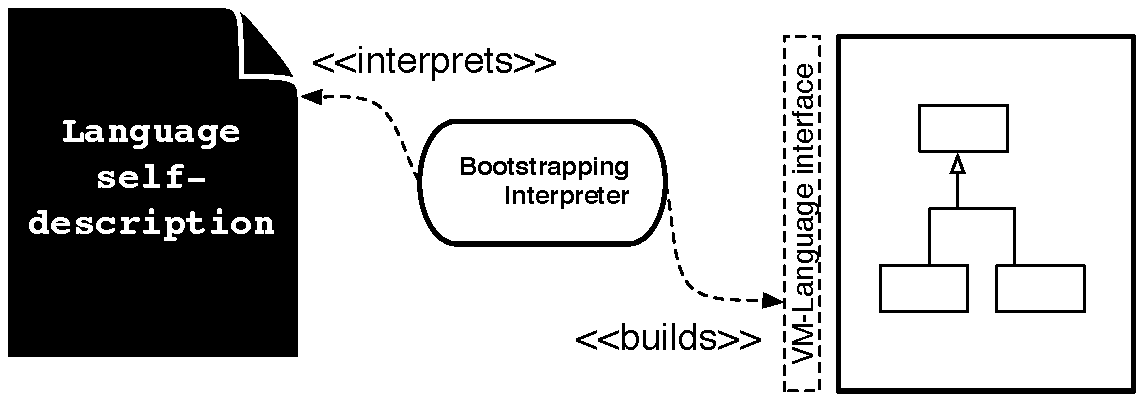
\includegraphics[width=.9\linewidth]{bootstrap_nutshell}
\caption{\textbf{Solution overview.} A bootstrapping interpreter uses the self-description in the language definition to build the language through the a clear \VM-language interface.\label{fig:bootstrapping_overview}}
\end{figure}

The main limitation of our approach is the \VM execution model. Our solution exposes a clear but fixed \VM interface that introduces a common denominator for each of the languages we bootstrapped. The co-evolution of language kernel and \VM will be addressed in future work and is out of the scope of this paper.

%============================================================================
\subsection{A Bootstrapping Process for Reflective Languages}

Bootstrapping requires a language kernel to be self-described. That is, there should exist a definition of the language expressed in the language it defines. This language definition includes the \textbf{base-level} entities of the language~(its classes and methods), and the \textbf{meta-level} entities with the means to define itself from scratch~(\eg a compiler or compiler interface to create methods and classes). The latter includes in addition the code of the bootstrapping process \ie the steps that must be followed to create a coherent and well formed language kernel~(Figure \ref{fig:language_definition}).

\begin{figure}[ht]
\center
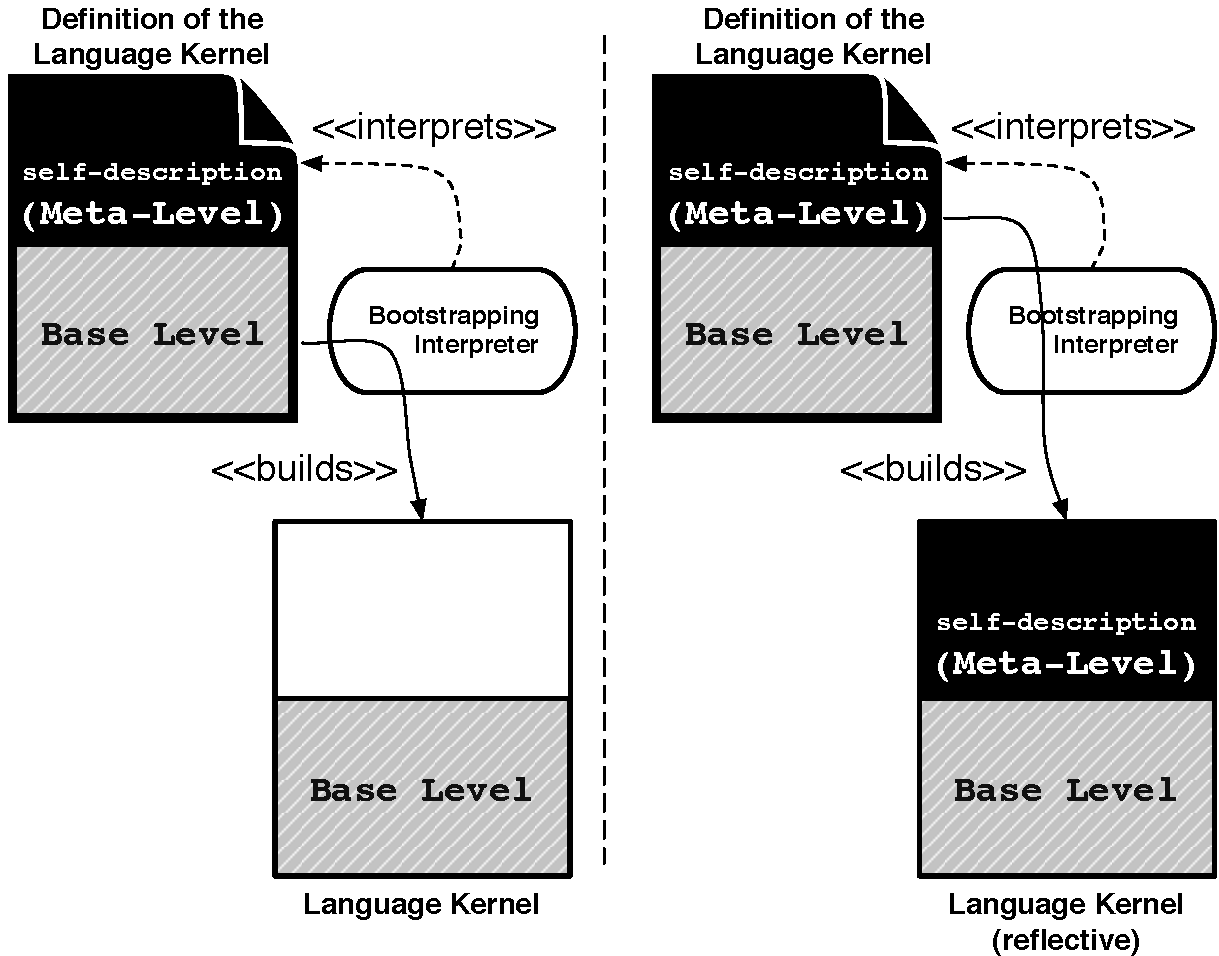
\includegraphics[width=.8\linewidth]{building_reflective_language}
\caption{\textbf{The language definition in the bootstrap process.} The bootstrapping interpreter uses the meta-level of the language to build the base-level of the language~(left-side). Afterwards, it may inject the meta-level to make it a reflective language~(right-side).\label{fig:language_definition}}
\end{figure}

Notice that although we use the language meta-level for bootstrapping purposes, it may just be needed at bootstrapping time and not at runtime. Bootstrapping does not require to inject the self-representation of the language into the language kernel. We consider that as a special case: a language kernel that includes its self-description is a \emph{reflective language kernel}.
A language that contains both introspection and full intercession facilities is a fully reflective language. A fully reflective language does not only have the minimal set of elements to run, but also the minimal to be autonomous: it can create classes and methods without any external component~(compiler, class builder, interpreter).

Thus, this language definition has direct impact on the design of the language we bootstrap. Figure \ref{fig:phases} shows the stages of a bootstrap process as it installs classes or packages inside the language kernel. When the bootstrap process starts, the language kernel is not yet able to execute code by itself \eg it cannot resolve the method lookup because the class hierarchy is not created. As we install packages or classes, we arrive at the point where the kernel contains already the minimal set of elements it needs for execution, the \emph{execution point}. Later on, we can install reflective features into the language to get inside the \emph{reflective spectrum} of languages. 

%When bootstrapping a reflective language, the language definition must ensure the causal connections that exist between the program and its representation~\cite{Maes87a}.


\begin{figure}[ht]
\center
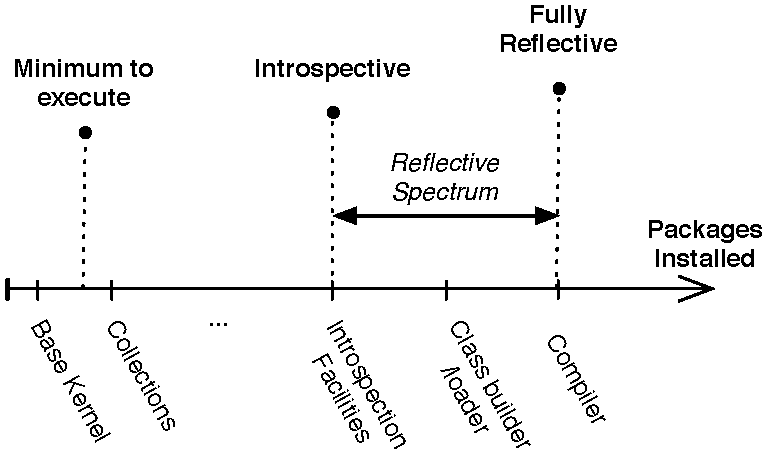
\includegraphics[width=.9\linewidth]{bootstrapping_phases}
\caption{\textbf{Bootstrap Phases.} Initially, a language kernel does not contain the minimal elements to execute code. As the bootstrap process installs elements, it reaches the point of execution where it can run autonomously. Later on, when (if) reflective features are installed, the process reaches the reflective spectrum, where a language kernel is considered reflective.\label{fig:phases}}
\end{figure}

%\begin{description}
%\item[The base-level language elements.]  We consider here those elements that are part of the \textbf{base-level}~(\eg basic language classes and libraries) of the language and also the ones in the \textbf{meta-level}~(\eg the reifications of the language runtime, a compiler interface, the class builder).
%
%\item[The meta-level language elements.]

\subsection{The process to create the language kernel}
The bootstrapping process requires a particular order as it sets up very interrelated dependencies~(sometimes meta-circular in the case of reflective languages~\cite{Stra14a,Chib96a,Maes87a,Smit84a}) amongst the language elements. The order and specifics to build the language must be described in the language definition so the bootstrapping interpreter can make use of it to orchestrate the process. This process presents also which are the elements that will be introduced into the built language: it is here where we decide if the output language kernel will be reflective or not.

Following we describe a bootstrap process we developed to bootstrap the Pharo language. A bootstrap process may be different for different languages, as they may contain different meta-models and concepts. As an example, Figure \ref{code:process} shows an excerpt of our particular bootstrap process applied to the Pharo language.

\begin{figure}[ht]
\begin{code}
Bootstrap >> bootstrap [
    "Create the basic language structures"
    nilObject := UndefinedObject basicNew.
    trueObject := True basicNew.
    falseObject := False basicNew.
    
    globalTable := GlobalTable basicNew.
    globalTable at: #GlobalTable put: smalltalk.
    
    SymbolTable initialize.
    
    "Solve the class creation bootstrapping issue"
    Class
        instVarAt: 4
        put: (FixedClassLayout
            withInstVars: #(superclass methodDict format layout ...)).
    
    "Create classes"
    ClassBuilder new
        superclass: nilObject
        subclass: #ProtoObject
        instanceVariableNames: ''.
    ClassBuilder new
        superclass: ProtoObject
        subclass: #Object
        instanceVariableNames: ''.
    ...
]
\end{code}
\caption{\textbf{Code (excerpt) of the Pharo language definition.}\label{code:process}}
\end{figure}

%In \cite{Poli13b} Polito et at. 
%we provided a detailed process to bootstrap an object-oriented reflective language such as Pharo. The bootstrap process is not the contribution of this paper. However, for the sake of completion and to aid the understanding of the rest of the paper, we briefly explain in this section the bootstrap process by the means of an example consisting in the bootstrap of the Pharo language. \gp{send them to read our report with the full blown process}


%\paragraph{Step 1: Generate the guest language AST definitions.}
%
%The builder takes as input the specification of the guest language, parses them and generates abstract syntax trees~(ASTs) of the new language's elements~(\eg classes and methods). 
%These AST objects provide to the bootstrap process with (a) the format and shape of classes and objects, (b) the source code of methods to be compiled inside the object space and used by the AST interpreter and (c) compile-time information such as instance and class variable names.

\paragraph{\textbf{Step 1: Create the first well-known objects}}\label{sec:create_nil}

When the bootstrap process starts, the bootstrapped language kernel is empty \ie there are no objects inside it. 
The first step of the process is to create the \ct{nil}, \ct{true} and \ct{false} objects needed for execution. It is important to create the \ct{nil} object first as the rest of the objects will have their fields initialized to it. \ct{true} and \ct{false} are required for code execution.
%%that are created inside the object space 
%will initially have their fields pointing to the \ct{nil} object from the guest language kernel. Then, the first object that the bootstrap process creates is the \ct{nil} object.
%
%In a class based object-oriented language\footnote{These same problems appear in the case of prototype based languages}, the expected way to create the \ct{nil} instance would be to instantiate it from its class. However, the \ct{nil} class does not exist yet in the guest language kernel. Creating it poses some recursive questions: (a) if the a class is an object, how could we create a class without another class for it? and (b) if that class must be initialized with references to \ct{nil}, how can we reference the correct \ct{nil} object if there is no \ct{nil} instance yet? To solve this issue, a \ct{nil} object is created in the guest kernel without linking it to a class, using an unsafe operation and breaking the language's invariants temporarily.

%An \emph{unsafe} \ct{createAnonymousObject} operation to create an object with no class. This operation takes as input the format describing the object to be created, creates the corresponding object, and outputs a mirror on that object. In our particular implementation, this operation introduces a temporary anonymous class in the guest and creates an object from it. This temporary class keeps some references to the \ct{nil} object from the host, breaking temporarily the isolation property. Using this operation, the guest \ct{nil} object is created. Later on, when the corresponding class of \ct{nil} is created, its class relationship is replaced, the temporary class is discarded (unreferenced and garbage collected), and the isolation is restored~(cf. Section \ref{sec:well_known}). The method responsible of the creation of the \ct{nil} object is shown in Figure \ref{code:nil_creation}. Figure \ref{fig:nil_creation} depicts the state of the guest language after this step.



%\begin{figure}[ht]
%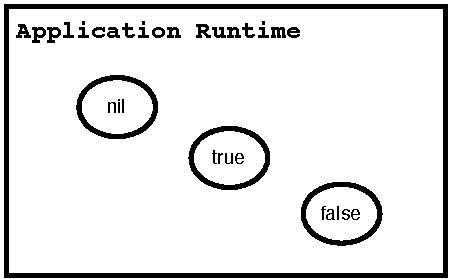
\includegraphics[width=.98\linewidth]{nil_creation}
%\caption{\textbf{State of the guest language after the creation of the classless nil object.} The \ct{nil} object is the only instance in the guest language. It is an object whose class is an anonymous class, marked in gray, pointing to the \ct{nil} object from the host.\label{fig:nil_creation} \cam{I would expect the anonymous class to appear outside the guest system rather than inside}}
%\end{figure}


\paragraph{\textbf{Step 2: Create basic language structures}}

The basic language structures of a language kernel is the minimal structure needed to create all the rest of the elements in the language. For example, the language may have a table of globally accessible objects, and a table of unique strings or symbols. These basic structures should be created from the very beginning, as the rest of the process can rely on them.
%
%
%To explain it by example, we take the well-know example of Smalltalk~(Figure \ref{fig:pharo_metaclass_metacircularity}). In Smalltalk each class has a metaclass, instance of a \ct{Metaclass} class. The \ct{Metaclass} class is an instance of a \ct{Metaclass} metaclass. According to this model, the \ct{Metaclass} class and \ct{Metaclass} metaclass should be created before any other class, and thus, it is for us the \emph{basic metacircularity}. It is worth saying that languages such as Pharo or Ruby~\cite{Mats01a} present similar models. \gp{In JavaScript... ?}
%
%\begin{figure}[ht]
%\begin{center}
%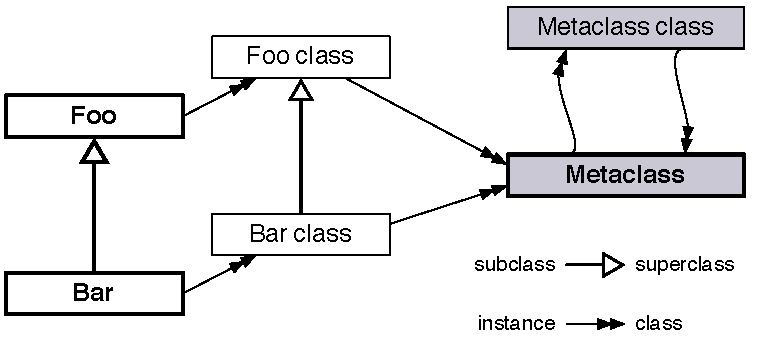
\includegraphics[width=.8\linewidth]{pharo_metaclass_circularity}
%\caption{\textbf{Metaclass metacircularity in Pharo.}\label{fig:pharo_metaclass_metacircularity}}
%\end{center}
%\end{figure}
%
%The creation of the first \ct{Metaclass} class and \ct{Metaclass} metaclass is mutually dependent: each one is an instance of the other, and thus, each one needs the other to be created. To overcome this, we use again the same strategy as for the \ct{nil} object. The builder creates the corresponding \ct{Metaclass} class and metaclass, not linking them to each other. Once both of them are available, we update their class links.

\paragraph{\textbf{Step 3: Create classes}}
We create all the classes that the language definition requires in the language kernel. The bootstrapping interpreter uses the corresponding class building mechanism in the meta-level of the language to create the corresponding classes from their descriptions. Methods are not yet installed in their classes.
%Creating a class is a complex operation at this stage. For example, a class has a name which is a symbol\footnote{a Symbol is a string unique in the system}, which in turn cannot be created yet because the Symbol class does not exist yet. Another example is the usage of complex collections such as Dictionaries in the class definitions for class variables.
%by taking each class' AST from the specification, instantiating a metaclass from the \ct{Metaclass} class and the corresponding class from the new metaclass.
% The \ct{asClassMirror} message is sent to the metaclass mirror, so the builder can instantiate the corresponding class from this metaclass. This sub step is shown in Figure~\ref{code:class_creation}. Once the bootstrap process creates all classes in this way, the guest language contains all its classes but they are still not initialized. Classes are yet not related between them and have no methods installed. Figure \ref{fig:class_creation} shows an example of the state of the guest language after this step is finished. 
%In this step the builder doesn't initialize all classes. It lets their fields referencing to the guest \ct{nil} object. No methods are installed yet.

%\begin{figure}[ht]
%\begin{code}
%newMetaclass := metaclass basicNew asClassMirror.
%newMetaclass format: aClassDefinition classSide format.
% 
%newClass := newClassMetaclass basicNew asClassMirror.
%newClass format: aClassDefinition format.
%\end{code}
%\caption{\textbf{Class creation inside the object space.} The mirror to the \emph{metaclass} allows the instantiation of a new metaclass. This new metaclass is afterwards used to instantiate the corresponding class. Each of these classes contain their corresponding formats. This task is repeated for all the classes defined in the specification. \label{code:class_creation}}
%\end{figure}
%
%\begin{figure}[ht]
%\begin{center}
%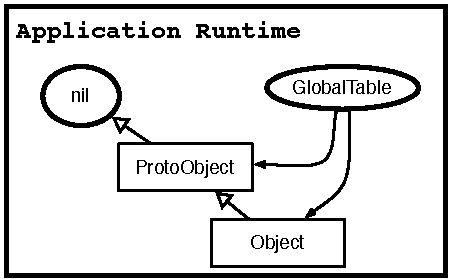
\includegraphics[width=.98\linewidth]{class_creation}
%\caption{\textbf{State of classes in the guest language after class creation.}  The metaclass metacircularity is set up. Other classes, such as \ct{Object} or the correct \ct{UndefinedObject} are instances of their respective metaclass, which in turn are  instances of \ct{Metaclass}. All slots of these classes~(in particular the slot indicating the \emph{superclass}) reference the guest \ct{nil} object. At this point, two \ct{UndefinedObject} classes exist in the guest, in gray the one created in section \ref{sec:create_nil} referencing to the host language, in white the one we created in this step. \label{fig:class_creation}}
%\end{center}
%\end{figure}

%\paragraph{Step 5: Initialize well-known instances.}\label{sec:well_known}
%
%In this step the well known instances of the language kernel are instantiated and initialized.
%We set the class link of the \ct{nil} object with its corresponding class which was created in the last step. We create also other well known instances such as the \ct{true} and \ct{false} objects.% The process uses the \ct{setClass:} operation of the mirrors to set the \ct{nil} object its corresponding class and restore the isolation of the new language. The \ct{true} and \ct{false} instances are instantiated using their corresponding classes in the object space. 
%The code executing this step is shown Figure~\ref{code:nil_fixation}. 
%After this step, \ct{nil} is not a \emph{classless} object anymore. Also, the guest language is \textbf{transitively closed}, although it is not completely initialized as shown in Figure \ref{fig:well_known_instances}.

%\begin{figure}[ht]
%\begin{code}
%theNil setClass: nilClass.
%theTrue := trueClass basicNew.
%theFalse := falseClass basicNew.
%\end{code}
%\caption{\textbf{initialising the nil, true and false instances.} Fixing the nil reference to the new nil class that was just created. The \ct{setClass:} operation of the mirrors is used. Also, the \ct{true} and \ct{false} instances are created by instantiating their corresponding classes. \label{code:nil_fixation}}
%\end{figure}

%\begin{figure}[ht]
%\begin{center}
%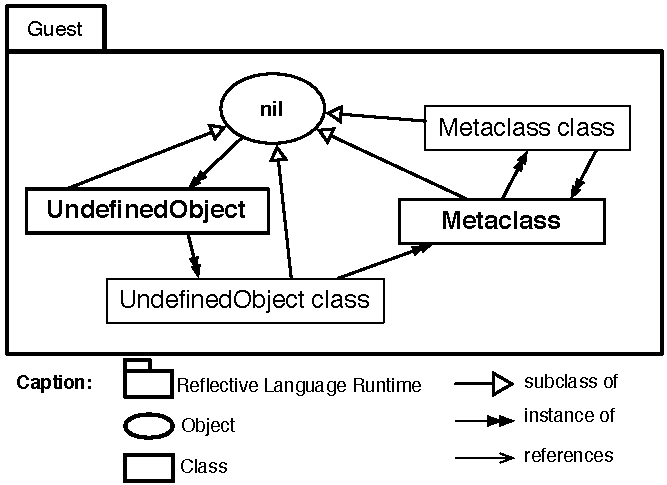
\includegraphics[width=.98\linewidth]{well_known_instances}
%\caption{\textbf{The guest language is finally transitively closed.} After setting the \ct{nil} object with its corresponding class from the guest language, the graph is transitively closed.\label{fig:well_known_instances}}
%\end{center}
%\end{figure}

%\begin{figure}[ht]
%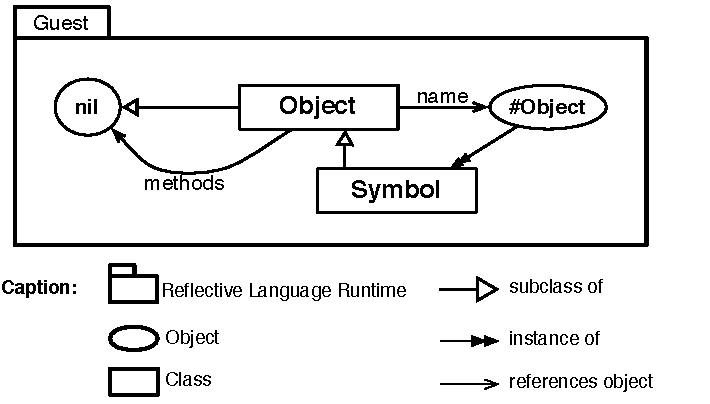
\includegraphics[width=.98\linewidth]{class_initialization}
%\caption{\textbf{State of classes in the guest language after class initialization.}  Each class references to its corresponding superclass. The superclass of \ct{Object} is \ct{nil} as it is the root of the inheritance chain. Class state is initialized~(\eg their names initialized as symbols) except their methods. \label{fig:class_initialization}}
%\end{figure}

\paragraph{\textbf{Step 4: Installing methods}}

We compile~(if needed) and install each of the methods present in the language definition into their respective classes. Method literals are bound to their corresponding literals or global objects (\eg classes).

%\begin{figure}[ht]
%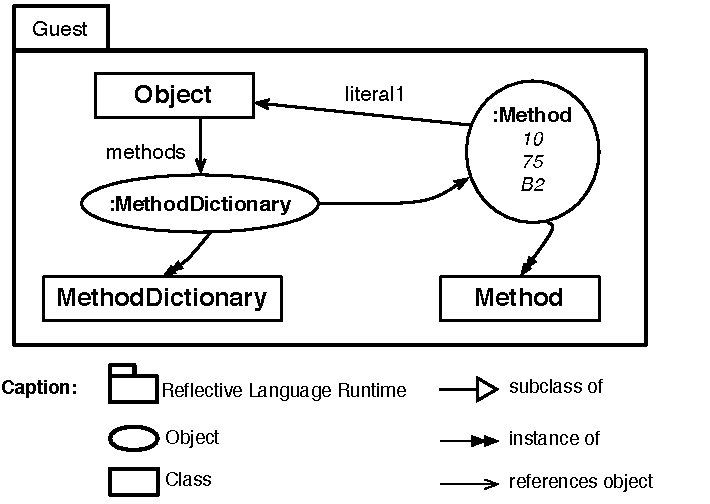
\includegraphics[width=.98\linewidth]{method_installation}
%\caption{\textbf{State of classes after method installation.} Each class has a method dictionary. Each method dictionary references the installed methods. A method object contains the bytecode and references the literals it uses.\label{fig:method_installation}}
%\end{figure}


\paragraph{\textbf{Step 5: initialization}}
%With all the classes and methods from the language specification installed, the structural part of the language is already set up. 
This last step consists in the execution of the class initialize methods to set up elements such as character tables, well-known float values~(\eg NaN or Infinity) and the thread machinery. This means that at this point, our language kernel should be able to execute code by itself.
\newline

While such a bootstrap is not difficult to express per se, it raises the question of how it can be executed. This is challenging especially, since for example we need classes to be defined to execute this exact bootstrap description. This question leads to ask ourselves about the infrastructure required to be able to manage this and other different bootstraps. The following section describes the infrastructure we built to solve this problem.

% ===========================================================================
\section{Bootstrapping with \Vtt}\label{sec:bootstrapping_infrastructure}

We implemented a bootstrapping infrastructure on \Vtt. In our solution, the bootstrapped language kernel will be created inside the virtualized runtime. This virtualized runtime is initially empty and a bootstrapping hypervisor will fill it with new objects before running the virtualized environment. The main component of the bootstrapping hypervisor is a \emph{bootstrapping interpreter}. The bootstrapping interpreter is a specialised AST interpreter that can execute the code available in the language definition under the initial absence of classes and objects~(Figure \ref{fig:objectSpaceOverview}).

%  on \emph{object spaces} and abstract interpretation~(cf. Figure \ref{fig:objectSpaceOverview}). An object space is a first class representation of an \emph{object runtime system}: it is an object that provide a high level API to manipulate an object runtime system. An object space \textbf{isolates} its represented object runtime system by using mirror objects~\cite{Brac04b}~(cf. Section \ref{sec:mirrors}). Abstract Syntax Tree~(AST) interpretation solves the remaining issues. First, the combination of object spaces and the AST interpreter allow multiple object runtime systems to co-exist and execute independently, overcoming the \textbf{unicity hyphotesis}~(cf. Section \ref{section:object_spaces} and Section \ref{sec:ast_interpreter}). Second, with AST interpretation we can execute code inside the guest language kernel, using the language specification as a source for both compilation and execution, \textbf{avoiding logic duplications}.
%
%In this section, we present how our solution supports the bootstrap process introduced in Section~\ref{sec:process} and solves our stated challenges. We provide the API of both our object spaces and mirror objects, and how our AST interpreter interacts with the object space infrastructure.

\begin{figure}[ht]
\center
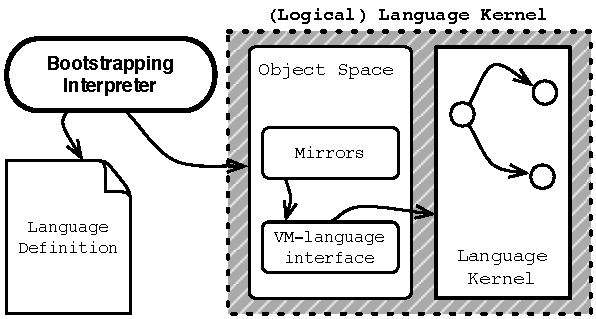
\includegraphics[width=.9\linewidth]{object_space_bootstrap_overview}
\caption{\textbf{Solution overview in \Vtt.} The virtualized runtime will contain the bootstrapped language kernel. A \emph{bootstrapping interpreter} executes the language definition on the virtualized runtime using the object space interface.\label{fig:objectSpaceOverview}}
\end{figure}

To support the bootstrapping process in the time our bootstrapping infrastructure provides with measurement of change impact in a scenario where changes are common and bootstrapping must be performed continuously~(Section \ref{sec:continuous_bootstrapping}). We achieve this by integrating the bootstrapping process in a continuous integration environment. The bootstrapping interpreter traces the execution of the bootstrap and can provide the language developer with feedback about the impact of his/her changes.

%\subsection{Virtualized Runtime for Bootstrapping}\label{section:object_spaces}
%
%With \Vtt, an Object-Oriented language bootstrap generates the language elements~(objects, classes, methods, threads) inside a virtualized runtime. For bootstrapping purposes, this runtime is initially empty. 


\subsection{The Bootstrapping Interpreter}\label{sec:ast_interpreter}

The bootstrapping interpreter is a virtual code interpreter that interprets code expressed in the bootstrapped language. The bootstrap process uses the bootstrap interpreter to execute the language definition inside the virtualized runtime before it reaches the execution point. Its design present the following important properties that allow it to achieve this:

\begin{description}
\item[Alternative method lookup.] Before reaching the execution point, the class hierarchy of the language kernel is incomplete, or part of its methods are not yet installed. The bootstrapping interpreter implements an alternative method lookup mechanism to allow message sending before we reach the execution point: methods are looked up in the definition of the language instead of the hierarchy in the language kernel; a mapping is kept between classes created in the language kernel and their definitions in the language definition to know where the lookup should start.

\item[Automatic class stubs.] The bootstrapping interpreter does also solve most of the well known bootstrapping issues~(\eg how to create a class before a class exists) in a generic way by using class stubs. When an inexistent class is needed during the bootstrap process, the interpreter creates an empty class to take its place respecting the \VM format for it. The interpreter will be able to create instances of this class and map it to its corresponding definition to perform the method lookup. This class cannot, however, initially perform reflective operations as it does not contain any reflective information. When the real class is created later on in the process, it replaces the stub. For this purpose, we extended the object space interface with one operation that allows the creation of an object whose class pointer is not initialized.

\begin{code}
objectSpace {
    mirror allocateObjectOfSize(int size);
}
\end{code}

\end{description}

\begin{figure}[!ht]
\center
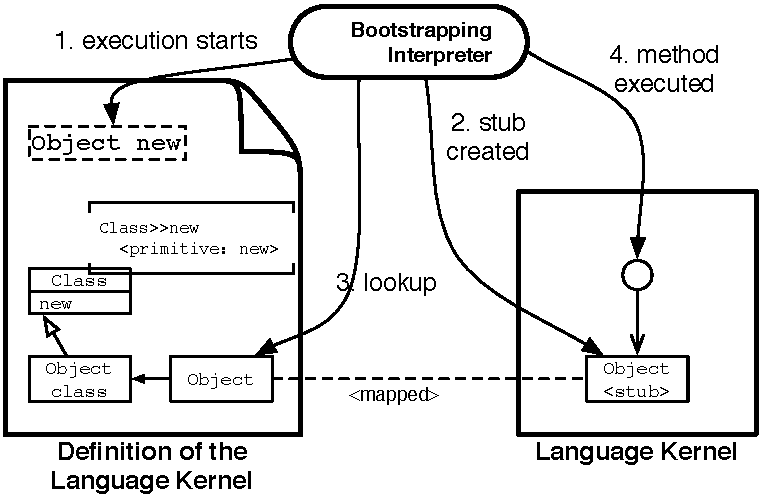
\includegraphics[width=.8\linewidth]{interpretation}
\caption{\textbf{The Bootstrapping interpreter in action.} A stub class is created for a non existent class. Each class is mapped to its description in the language definition. The lookup is then performed inside the language definition. Once the method is found, it is executed inside the language kernel.\label{fig:interpretation}}
\end{figure}

Figure \ref{fig:interpretation} illustrates with an example the behavior of the interpreter, particularly in the execution of the \ct{"Object new"} expression. First, if the class \ct{Object} does not exist, it create a stub \ct{Object} class and maps it to its corresponding definition in the language definition. To interpret the \ct{new} message, the interpreter performs the method lookup from the class of the object in the language definition. As the class from the language kernel and the language definition are mapped, the interpreter knows where to start the method lookup. Finally, the found method is executed in the language kernel and an instance of the \ct{Object} class is created.



By using the bootstrapping interpreter to bootstrap, all the executed logic comes from a single source: the language definition. This avoids  major code and logic duplications between \VM and language, as the only one point for extension or modification of the bootstrapped language is its definition. Figure~\ref{code:logic_dup3} illustrates how we can use the interpreter to use the \ct{Dictionary} definition from the language and avoid duplications in native code as shown in \chapref{background}.


\begin{figure}[ht]
\begin{code}
Bootstrap>>createDictionaryWith: n
    "Create a dictionary in the new language kernel"
    ^ interpreter
            execute: 'Dictionary new: size'
            binding: { 'size' -> n }.
\end{code}
\caption{\textbf{Avoiding logic duplications with the bootstrapping interpreter.} This example shows how the bootstrapping interpreter does not duplicate the logic of the \ct{Dictionary>>initialize} method, but uses it instead.\label{code:logic_dup3}}
\end{figure}


\subsection{Continuous Bootstrapping}\label{sec:continuous_bootstrapping}

Building continuously a language kernel provides the language engineers with the same benefits of continuously building another application: automated integration and testing, quick and continuous feedback on the applied changes. This continuous feedback should give the language developer with the information and tools to resolve conflicts and problems: it should clearly show which was the \emph{impact} of such change in the process. A change introduced in the language impacts directly on the definition of the language~(Figure \ref{fig:impact}). The changed definition is used in turn by the bootstrap process to bootstrap the new version of the language kernel, thus the change has also an indirect impact on the bootstrapped language. 

\begin{figure}[ht]
\center
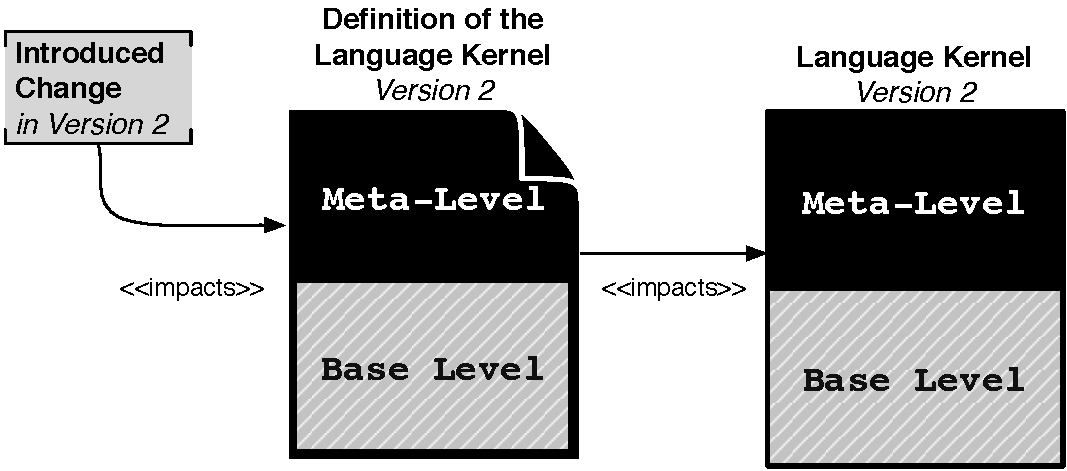
\includegraphics[width=0.7\linewidth]{impact}
\caption{\textbf{How a change impacts the bootstrap process.} A change in the language may impact directly in the definition of the language, which in turn impacts in the bootstrapped language.\label{fig:impact}}
\end{figure}

However, not every change in the language definition may impact the bootstrap process: not all the code in the language definition is used during the bootstrap~(\ie executed by the bootstrapping interpreter) and not every change impacts in the behavior of the process (\eg changing the set of final classes introduced by the bootstrap). With this purpose we introduced as a second output of our bootstrapping interpreter, an execution trace containing all the language elements that were used to bootstrap: any change on these elements may have an impact on the process. Then, to produce useful feedback for the changes made by a language developer, an \emph{impact resolver} measures the impact of a change in the bootstrap process by comparing the introduced change to the previous bootstrap execution~(Figure \ref{fig:resolving_impact}).

Our bootstrapping infrastructure measures the impact by making a diff between the traced and changed language elements. In case a change breaks the bootstrap process, the language engineer has enough information to spot the problem and act on it.

\begin{figure}[ht]
\center
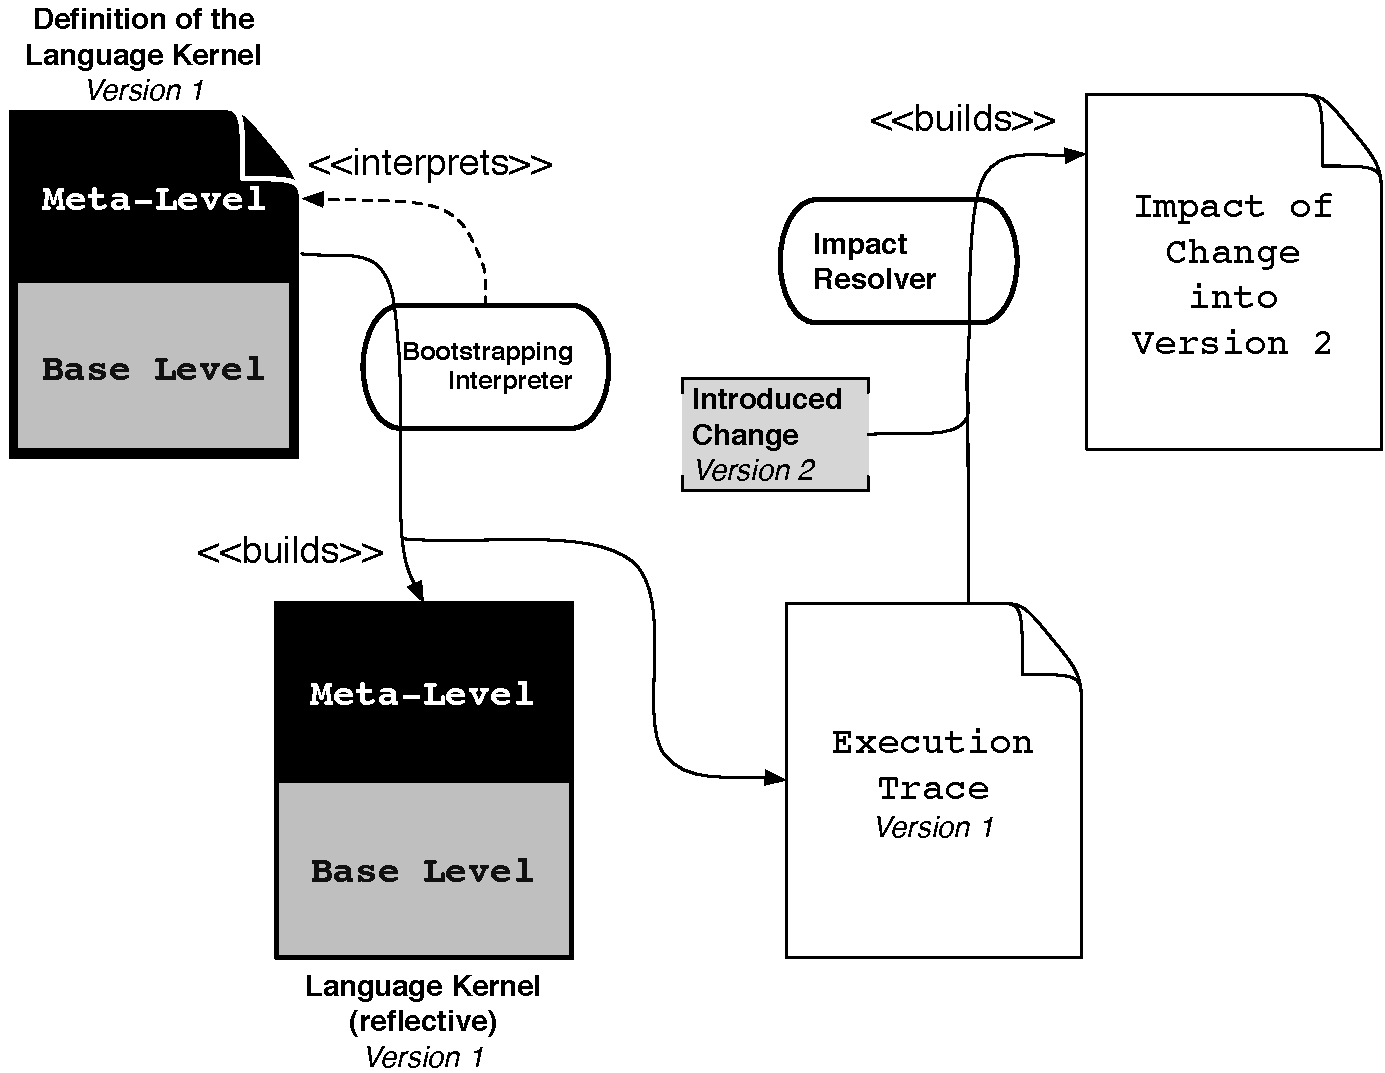
\includegraphics[width=.8\linewidth]{resolving_impact}
\caption{\textbf{How a change impacts the bootstrap process.} The bootstrap process execution is traced. An impact resolver decides if the introduced change will impact in the bootstrap process or not.\label{fig:resolving_impact}}
\end{figure}

% ===========================================================================
\section{Validation} \label{sec:bootstrapping_validation}

In this section we present our results while bootstrapping three different three different case study languages.
As all our languages share the same \VM, we start this section by describing the execution model of this \VM and its impact on the bootstrapping languages.
To reuse the parsing infrastructure and the bootstrapping interpreter, the three bootstrapped languages share also the same syntax: a Smalltalk syntax. Although these similarities, each of the three language kernels possess different model and semantics: Pharo is a fully-reflective language composed of classes and traits with first class slots and object layouts \cite{Verw11a}; \emph{Metatalk}~\cite{Papo11a} is a language that fully decomposes the meta-level from the base-level using mirrors, allowing us to bootstrap a reflective and a non-reflective version of it; \emph{Candle} is a partially reflective \ct{Smalltalk-80} based mini-kernel that includes introspection and some self-modification features. Figure \ref{fig:languages_spectrum} shows how these three languages are placed in the language spectrum.% These results show that our process can produce different systems when fed with different specifications. The resulting bootstrapped systems are available at \url{http://ci.inria.fr/rmod/view/Oz/}.

\begin{figure}[ht]
\center
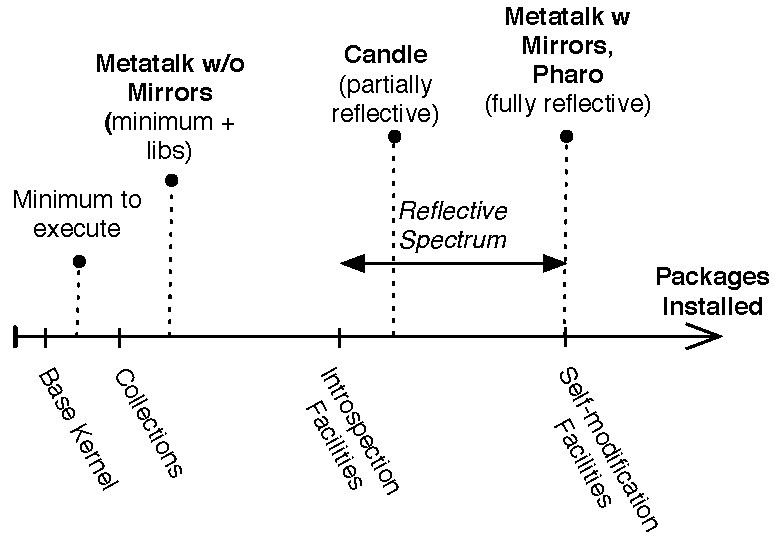
\includegraphics[width=.8\linewidth]{languages_by_reflectiveness}
\caption{\textbf{Bootstrapped Languages Spectrum.} How the languages we bootstrapped are placed in the phases and reflective spectrum. In particular, Metatalk with and without its mirrors is in different extremes of the spectrum.\label{fig:languages_spectrum}}
\end{figure}

Finally in this section we present some measurements. To keep bootstrapping practical, we optimized the critical parts of the process for both the language user and the language engineer. On one side language users do not usually search to modify the language kernel but to use it, independently of the language initialization process it provides. To suit this scenario we do not build the language kernel each time: we generate a snapshot with a cached version of it. On the other side we find language designers/engineers whose job is to change the language kernel. For them the bootstrap process must provide with an acceptable development cycle for activities like debugging. With this case in mind, we optimized the \emph{bootstrapping interpreter} with a dynamic compilation technique. Each of the measurements we present below were made on a 2.2 Ghz Intel Core i7 machine with memory 8 Gb 1333 Mhz DDR3.


\subsection{Pharo Execution Model in a Nutshell}\label{sec:pharo_execution_model}

To understand the common denominator between the three language kernels we bootstrapped, we describe briefly the execution model imposed by the Pharo \VM. The Pharo \VM features a bytecode-based stack interpreter with a generational garbage collector and a JIT compiler. For the interested reader, several publications describe its details and how it evolved during time~\cite{Gold83a,Inga97a,Mira11a}. On the execution model side, this \VM imposes us the following contract:

\begin{description}

\item[Object Format.] All objects in a Pharo \VM have a header and a list of fields. The object header is one, two or three words long and describes amongst others how large is the field list of the object, if those fields contain weak or strong pointers, and which is the class of the object.

\item[Object Model.] The Pharo \VM enforces, in its lowest level, a class-based object oriented model with single inheritance. Each object has a reference to its class~(that appears inside its header). Additionally, each class has three mandatory fields: the class format is used to create new instances and the class' superclass and a method dictionary are used during the method lookup. The \VM during its execution does not enforce the existence of metaclasses nor a particular class hierarchy. This simple model allows one to implement language extensions such as Traits~\cite{Scha03a}.

\item[Bytecode set.] The Pharo \VM constrains methods to a single bytecode set, based on its stack machine. This means that every language that is meant to run on top of this \VM must be compiled to this bytecode set, independently of its original syntax and semantics. 

\end{description}

\subsection{Case Study I: Pharo}\label{sec:bootstrap_pharo}

Pharo~\cite{Blac09a} is an object-oriented reflective Smalltalk-inspired programming language. As it is a Smalltalk-80 inspired language, its class model includes implicit metaclasses: each class has its own metaclass, an instance of \ct{Metaclass}. Pharo also extends the execution model its \VM provides with traits~\cite{Scha03a} and class extensions~(\ie the ability to add methods to a class that belongs to another package). Finally Pharo has first class instance variables (slots) structured in object layouts \cite{Verw11a}. Figure \ref{fig:pharo_simplified_model} shows how the elements of the language are related to each other; the diagram is not meant to reflect the actual class graph but the language concepts.

\begin{figure}[ht]
\center
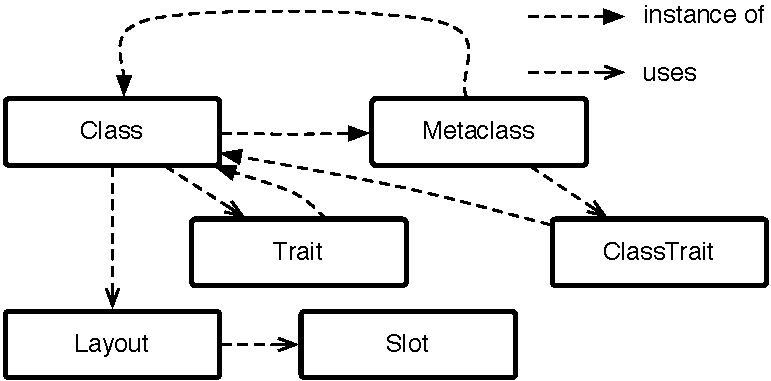
\includegraphics[width=.7\linewidth]{pharo_simplified_model}
\caption{\textbf{Simplified Pharo object model schema.} In Pharo each class has a metaclass. Metaclasses are defined circularly. Both classes and metaclasses makes use of trait objects to define part of their behavior. Classes also has layout that organises first class instance variables (slots). This schema does not represent the actual object graph, but a simplified picture.\label{fig:pharo_simplified_model}}
\end{figure}

Pharo is a fully-reflective language, placed at the end of the reflective spectrum. The Pharo language includes introspection in the kernel itself, and also self-modification stratified in three levels: object mutation facilities, a class builder and a compiler. The main challenge in Pharo is that the kernel itself of Pharo is defined by Traits: \eg the Trait class uses a Trait. First class slots also add to the self-description of the language. This introduces new bootstrapping issues that must be resolved at bootstrapping time.

%Our resulting language kernel includes the packages defining Pharo's class model, traits, collections, the process scheduling library, the compiler and the class builder. The two latter allow the system to be extensible without external tools. With this selection we bootstrapped a language kernel that represents the 19\% of the original language kernel.
%The memory  the resulting bui language is 2MB, contrasting its 22MB original counterpart. \gp{remeasure it. Do we care about size?}

%Regarding its health, the boostrapped kernel can be tested using the SUnit testing framework.
%Unit tests of the kernel itself are loaded using the binary loader and run in the new system.
%Using this same mechanism, core packages like the compiler are able to be tested isolated from other libraries.

%A peculiarity of this system is that it is capable of bootstrapping a copy of itself.
%This is achieved by loading the binary packages of hazelnut and using it's own specification in the building process.
%Regarding the size of our obtained kernel, which is certainly not yet the minimal possible, our results shows that the design of the language kernel should be refined to create an even cleaner version.

\subsection{Case Study II: Metatalk} \label{sec:bootstrap_metatalk}

Metatalk~\cite{Papo11a} is a reflective language where reflection is fully decomposed in explicit meta-objects, namely mirrors~\cite{Brac04b}. Metatalk makes the usage of reflection explicit: a program's execution takes place in the base-level of the language kernel, and it jumps to a meta-level when a mirror is used. Metatalk class model is simpler than Smalltalk's class model. It does not impose metaclasses. Instead, all classes are instances of the single \ct{Class} class. If there is a need for metaclasses~(to share behavior between classes), the developer can write its own explicit metaclasses~(Figure \ref{fig:metatalk_simplified_model}).

Metatalk mirrors decompose reflective behavior as well as the language meta-information \ie class' names, field order and names amongst others are part of its mirrors, and thus, they belong to the meta-level. When there is not a need for reflection, a Metatalk program can discard its meta-level with all the meta-information in it. This decomposition allows us to bootstrap Metatalk with or without its meta-level. This results in two different language kernels: Metatalk base-level has no reflection at all, while Metatalk with both the base and the meta level is a fully-reflective language.

\begin{figure}[ht]
\center
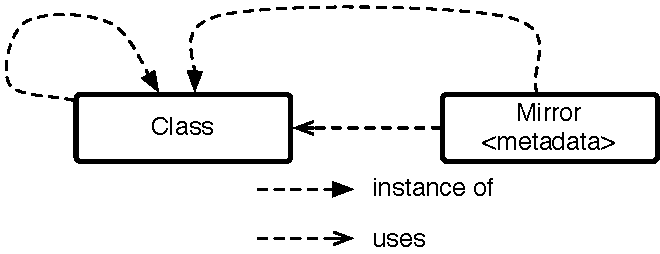
\includegraphics[width=.7\linewidth]{metatalk_simplified_model}
\caption{\textbf{Simplified Metatalk object model schema.} In Metatalk classes have no implicit metaclass. All classes share the same class. Mirrors are simple objects, thus instances of classes, that reflect on a class and contain their metadata. This schema does not represent the actual object graph, but a simplified picture.\label{fig:metatalk_simplified_model}}
\end{figure}

Metatalk's can be bootstrapped in two different ways. A non-reflective bootstrap initializes only the main classes of the language but does not create its meta-level. The non-reflective bootstrap does not contain mirrors. A second bootstrap creates a reflective Metatalk, which based on the latter one introduces the mirror instances with their corresponding metadata. We could bootstrap easily Metatalk in such a way due to the clear decomposition of its reflective elements. 

%%%%%%%%%%%%%%%%%%% Case of study and Results 2 %%%%%%%%%%%%%%%%%%%%
\subsection{Case Study III: Candle} \label{sec:bootstrap_candle}

Candle is a Smalltalk-based language with a micro language kernel. Its class model includes implicit metaclasses as Smalltalk's and Pharo's one. However, Candle has no support for traits or slots~(Figure \ref{fig:candle_simplified_model}). We built Candle's language kernel by adapting MicroSqueak~\cite{Malo11a} to run on top of the Pharo \VM. This micro language kernel was designed with the explicit goal of being the minimal distribution for the Squeak Smalltalk language.

\begin{figure}[ht]
\center
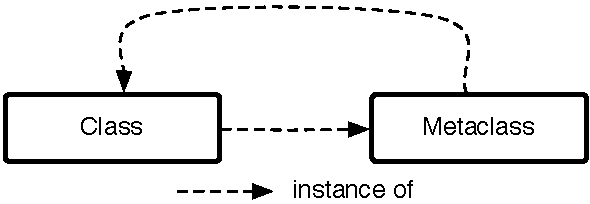
\includegraphics[width=.6\linewidth]{candle_simplified_model}
\caption{\textbf{Simplified Candle object model schema.} Candle follows a more traditional Smalltalk-80 model. In Candle each class has a metaclass. Metaclasses are defined circularly. There are no traits. This schema does not represent the actual object graph, but a simplified picture.\label{fig:candle_simplified_model}}
\end{figure}


Candle is a partially reflective language defined by a total of 49 classes and a reduced set of methods. Candle includes a minimal core of the language, a basic collection library and basic file IO support. It also provides with object introspection and mutation facilities. It does not include, however, a class builder or compiler to extend itself.%A bootstrapped Candle kernel presents a memory footprint of 80KB, with potential applications in embedded devices with little available memory.\gp{remeasure it. Do we care about size?}

\subsection{Measurements}

In this section we present the benchmarks we did to measure the bootstrap time of each of our three languages using our standard infrastructure. Table \ref{tb:measurements} shows the time to bootstrap each of the three languages using an unoptimised AST interpreter. This time comprehends the entire bootstrap process: from parsing the code in the language definition to its complete setup. We executed each of these benchmarks 10 times. The results table puts also the results in context: it presents how many code entities~(classes, traits, mirrors) and methods are built for each language. Notice that the bootstrapping time depends on the amount of elements it builds and also on their complexity. For example, creating a class in Pharo involves a biggest graph of objects than in the other two languages (because of the introduction of traits and class layouts). Section \ref{sec:optimisations} introduces two optimizations we did based on these measurements, that focus on the startup time and the development cycle of the bootstrap. 

 \begin{table}[ht]
 \small
 	\centering
 	\begin{tabular}{|l|c|c|}
			\hline
			\textbf{Language}
			& \xspace\textbf{Code entities / Methods}\xspace
			& \xspace\textbf{Bootstrap time}\\
		\hline
		Pharo & 626* / 6812 & 9004756ms +/-621265 \\\hline
		Candle & 100* / 875 & 86747ms +/-8060 \\\hline
		Metatalk w/o mirrors & 25 / 114 & 957ms +/-112 \\\hline
		Metatalk reflective & 58* / 166 & 13697ms +/-61 \\\hline
 	\end{tabular}
		\vspace*{0.2cm}
 	\caption{\small\textbf{Building Benchmarks.} Comparing the execution time of the bootstrapped languages using AST interpretation and partial evaluation. (*) Pharo and Candle have implicit metaclasses, meaning that for each created class, an associated metaclass is created even if not necessary. Metatalk introduces a mirror object for each of the classes in the language.\label{tb:measurements}}
 \end{table}

We can observe from our measurements that bootstrapping Metatalk takes in average 1 second if no mirrors are created and 13 in the reflective Metatalk case. Candle bootstrap is slower, in the order of 1 minute and a half, mainly because it contains eight times more methods than the Metatalk. We can see that a plain AST-based bootstrapping interpreter has a a bigger impact in the bootstrap time if the language contains complex structures to initialize.  Indeed, creating a Pharo class using the AST interpreter is an operation that takes in average 17 seconds, because each class contains a reification of its memory layout and slots~\cite{Verw11a}. This problem is aggravated by the high amount of classes and methods in this language definition.

Particularly about bootstrapping Pharo, a lack of modularity of the language impacts in the amount of code elements we have to build. Pharo's language kernel is historically a monolithic system which precludes us to build a minimal system. In fact, the Pharo language kernel we are bootstrapping represents a subset of the full Pharo language as it is distributed.

\subsection{Optimisations}\label{sec:optimisations}

To be useful in practice, we understand that the bootstrap process should have the following two properties: (a) be fast enough to provide a good feedback loop and allow debugging to the language engineer and (b) provide a short startup time for the language users. Optimising a bootstrap process is indeed a challenge since we cannot optimise it statically by fixing the meta-level semantics, as changing them is the main purpose of the bootstrap. In the following sections we show how snapshotting and dynamic compilation aid in these two optimisation scenarios. 

\begin{description}
\item[Enhancing Bootstrap Time: Dynamic Compilation.]
Since the main purpose of the bootstrap process is to easily change the meta-level semantics and structure of the language entities we cannot fix them statically to optimize them. In exchange, we chose to optimize the interpretation cycle using a dynamic compiler. The dynamic compiler compiles the interpreted code on demand. This compiled code is cached and executed directly on the \VM bypassing the interpretation step in following executions. We implemented dynamic compilation to optimize Pharo as it presents the worse of our results~(cf. Table \ref{tb:dynamic_compilation}). We reduced the total bootstrap time by a factor of 2.85. Additionally, we observed a mayor improvement on class creation, where the time improves from 17 to less than half a second. Class creation has a great impact on the Pharo's total bootstrap time, as it is executed 313 times. Contrastingly, the initial setup of the language structures~(\eg the symbol and character table, the initial threads) is executed only once where the cost of our dynamic compilation implementation increases the execution time. Please notice that the current implementation does not optimize method compilation nor parsing, meaning there is still a room for improvement.

 \begin{table}[ht]
 \small
 	\centering
 	\begin{tabular}{|l|c|c|c|}
			\hline
			\textbf{Case}
 			& \textbf{AST Interpretation}
			& \textbf{Dynamic Compilation}
			& \textbf{Gain}\\
			&&& \textbf{Factor}\\
		\hline
		Total Bootstrap & 9004756ms +/-621265 & 3158525ms +/-219334 & 2.85x\\\hline
 		Initial Setup& 247621ms +/-9875 & 319630ms +/-40333 & 0.77x\\\hline
		Creation of one class & 17216ms +/-1401 & 432ms +/-189 & 39.85x\\\hline
 	\end{tabular}
	\vspace*{0.2cm}
 	\caption{\small\textbf{Comparison of bootstrap time in absence and presence of dynamic compilation.}\label{tb:dynamic_compilation}}
 \end{table}

\item[Optimising Startup Time: Snapshotting.]\label{sec:snapshot}
The user of a programming language is concerned about writing applications that run on this programming language instead of changing the programming language. From a user perspective the initialization of the language is transparent within the startup of an application. It should be however fast and ensure always the same state.
The language initialization present in state of the art \VMs~(Section \ref{sec:intro}) provides both properties. Bootstrapping, in the sense of this paper, turns this process slower due to the interpretation step.

For language users, we overcome this slow-down by \emph{caching} the result of our bootstrap process in a snapshot. Thus, we bootstrap a language kernel only when we change it, and otherwise we load the cached version. Caching keeps both properties of application startup: it guarantees the same state and it is faster. Table \ref{tb:startup} shows a comparison in the startup time of our \VM loading Pharo and Candle using snapshots, in contrast with Ruby. We measured the startup times by running each of them 10 times and making an average. From the results, we observe our startup time is bigger than ruby's but still reasonable, under the half of a second.

 \begin{table}[ht]
 \small
 	\centering
 	\begin{tabular}{|l|c|}
			\hline
			\textbf{Language}
 			& \textbf{Startup time}\\
		\hline
		Ruby &  64ms +/-7.1\\\hline
		Pharo & 280.8ms +/-3.4\\\hline
		Candle & 186ms +/-7.6\\\hline
		Metatalk w/o mirrors &202ms +/-13\\\hline
		Metatalk reflective &205ms +/-11\\\hline
 	\end{tabular}
	\vspace*{0.2cm}
 	\caption{\small\textbf{Startup time in perspective.} Comparing the startup time of a ruby application with the same in Pharo or Candle using a snapshot.\label{tb:startup}}
 \end{table}

Implementation-wise, the snapshot we used is a memory dump of the \VM heap. This heap will contain all the objects, classes and methods we created during the bootstrap. At load time, the memory dump is restored into memory and the \VM internals are re-configured to use this heap using the \VM setup interface~(Section \ref{section:object_spaces}). This idea is the same used by languages such as Smalltalk, Lisp, Javascript in V8 or the JikesRVM~\cite{Alpe00a}. Loading a binary image is as fast as reading the file and putting its contents inside the \VM's heap.

\end{description}

% ===========================================================================
\section{Conclusion and Summary}

Bootstrapping is commonly known by its usage on compiler building, where a compiler can compile itself.
It can be generalized to the introduction of any software system to its own building process.
A bootstrap process allows us to easily change this system as it is expressed in terms of itself, taking advantage of its abstractions and tools.

In this chapter we explored the bootstrap of an object-oriented language using \Vtt. By using \Vtt we can easily modify the bootstrapped language runtime even when it is empty. A virtual code interpreter, the bootstrapping interpreter, allows the execution of the language definition in an initially empty virtual runtime. On one side, it overrides the method lookup mechanism to look for method ASTs inside the language definition instead of the half-built bootstrapped language. On the other side it solves the bootstrapping issues by automatically creating class stubs and replacing them once we create and install the real classes.

We validated our bootstrap process by bootstrapping three different object-oriented languages. These three languages have key differences between them: a minimal small-talk with implicit metaclasses, the core of the Pharo language which is defined by traits, and finally Metatalk which decomposes reflection from the base level and stores meta information in the meta level of the language. These three languages run on top of the Pharo Virtual Machine. We showed also that bootstrapping can be applied in a real environment. A fast startup can be achieved by caching the language kernel and a fast development cycle can be obtained by optimizing the bootstrapping interpreter.

The main limitation of our approach is that we don't address the co-evolution of language and VM. A co-evolution implies changing not only language and VM but also their interface. We expect to address these issues in future work and see what the introduction of a metacircular-programming framework implies in this regard.

% =============================================================================
\input{chapter-footer.tex}
\input{chapter-header.tex}
% ===========================================================================
\part{Tailoring: Automatic Extraction of Application Runtimes}
% ===========================================================================
\chapter{Run-Fail-Grow: Dynamic Tailoring}
\chaplabel{chap:rfg}
\minitoc
% ===========================================================================
\introduction
% ===========================================================================



This chapter describes the \emph{run-fail-grow} (RFG) technique: an alternative solution to dead code elimination that identifies the code units that are actually used in an application during runtime~(Section~\ref{sec:rfg_model}).
Using RFG, we launch a \emph{reference} application containing all code units~(base libraries, third party libraries and application code) and a \emph{nurtured} application runtime containing a \emph{seed} \ie a minimal set of code units we want to ensure in our application.
RFG generates an application runtime by ``growing'' the nurtured application into a deployable specialized version of the reference application. 
RFG runs the nurtured version of the application and feeds it with the code units that were detected missing through failures~(Section \ref{sec:rfg_example}).

The resulting deployable application only embeds the seed and used code.
By carefully choosing the seed, the user configures the scope of the tailoring process making possible different levels of tailoring.
For example, a seed that includes all base libraries makes the tailoring process only select used code in the application-specific part; whereas an empty seed makes the tailoring process select used code in all parts: base libraries, application libraries and application-specific part~(Section \ref{sec:seeds}).
% For example, if the seed includes the language base libraries, it ensures that the deployed application will have it all whereas an empty seed will result that only part of the base libs 
% Afterwards, deployment units are created from this shrank application to only contain the used code units.
% Using these compacted deployment units leverages the targeted device limitations. 

The dynamic nature of our solution allows its usage in dynamically-typed languages, and applications using reflection. Our solution does not need to modify the original application thanks to the use of \Vtt runtime virtualization.
It also successfully deals with applications that make use of programming language features such as reflection or open classes.

We developed Tornado, an RFG implementation based on \Vtt~(Section~\ref{sec:rfg_implementation}). In Tornado, the nurtured application resides inside a virtualized runtime. With \Vtt, we can monitor the execution of the nurtured application to detect whether a code unit is missing or not. Using \Vtt's mirrors we can also install the required code units.

\section{Run Fail Grow: Dynamic dead code elimination}\label{sec:rfg_model}

We propose a tailoring technique we named run-fail-grow~(RFG). Briefly, RFG works by launching a \emph{reference} application encompassing the full application with all its code units~(base libraries, third party libraries and application code) and a \emph{nurtured} application that has only part of its required code units installed. The nurtured application is run, and when a failure is detected because it misses a code unit, we install into it the corresponding code unit from the reference application. Thus, the nurtured application grows progressively as missing code units are found and solved.
Once finished, the nurtured application is ready to be deployed on target devices. Figure~\ref{fig:runfail} depicts the basics of our run-fail-grow approach.

\begin{figure}[ht]
\begin{center}
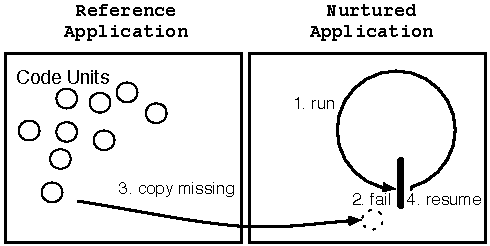
\includegraphics[width=.7\linewidth]{runfail}
\caption{\small \textbf{Application tailoring with a run-fail-grow approach.} We~(1) run the nurtured application and~(2) detect the missing units on failure. For each failure,~(3) we copy missing code units from the reference application and then~(4) the execution is resumed (just before the failure point) until the process finishes. \label{fig:runfail}}
\end{center}
\end{figure}

On one side, we start the reference application and pause it at the point where either it contains all its collection of code units, either we can load them dynamically~(under a lazy loading strategy). The reference application remains paused to avoid to mutate its state during the tailoring process. Pausing consists in suspending all processes and threads from the application.

On the other side, we fill initially the nurtured application with the \emph{seed} \ie the set of code units that we want to ensure in the final application. This seed allows us to specify the level of specialization of our deployable application.
By using a seed that contains all base libraries, RFG will only affect the application specific code units and third-party libraries.
However, by using an empty seed, it will also tailor base libraries~(cf. Section \ref{sec:seeds}).

Running the nurtured application consists in two main steps. We first install in the nurtured application one or more \emph{application's entry points} in the form of threads, and then we resume them.
The execution of these entry points results into sending messages to objects in the seed. These messages will signal \emph{missing code failures} when the respective classes and methods to resolve the message are not available.
We detect the missing code failures and solve them by fetching the needed code units from the reference application and install them into the nurtured application. RFG installs only code units on demand \ie the content of installed classes and objects is not installed until it is actually needed; methods are not installed until they are invoked.
The process repeats until we end it explicitly. As part of the process we can interact with the application under construction through \eg its UI. These interactions may signal more missing code failures, complementing the tailoring process. Ideally, the nurtured application reaches a stable point where it needs no more code units.
The nurtured application is then ready for deployment.

The dynamic nature of RFG tackles all our challenges. Missing code units are detected and resolved at runtime, where two main elements are available: the exact messages that are sent with their corresponding receiver and arguments, and their concrete types\footnote{We consider the exact class of an object its concrete type}. The methods and classes to install can be easily deduced from the available concrete types, \emph{without depending on type declarations nor their inference}. RFG \emph{takes into account the configuration of the application} such as the ones present in files, since the code that reads and interprets them is actually executed, without the need of custom code for them. \emph{Reflection is supported for free} since reflection invocations are treated as simple message sends and executed as any other code, and strings composed dynamically by the application are available at runtime. 


%%%%%%%%%% 


\section{Run-Fail-Grow through an example}\label{sec:rfg_example}
We illustrate in this section the ideas behind RFG with the example introduced originally in~\chapref{state_tailoring}~(cf. Figure \ref{fig:code_example_again}). For the sake of clarity, in this example we will tailor the application's code units only~(\ie not the base libraries). This means that in this example the seed includes the base libraries.

\begin{figure}[ht]
\begin{code}
MainApp>>start
    logger := StdoutLogger new.
    logger log: 'Application has started'.
    "do something"
    logger log: 'Application has finished'.

!\unusedcode{StdoutLogger>>newLine}!
!\unusedcode{~~~stdout newLine.}!

StdoutLogger>>log: aMessage
    stdout nextPutAll: Time now printString.
    stdout nextPutAll: aMessage.
    stdout newLine.
    
!\unusedcode{RemoteLogger>>log: aMessage}!
!\unusedcode{~~~| socket |}!
!\unusedcode{~~~socket := self newSocket.}!
!\unusedcode{~~~socket nextPutAll: Time now printString.}!
!\unusedcode{~~~socket nextPutAll: aMessage.}!
!\unusedcode{~~~socket newLine.}!

!\unusedcode{RemoteLogger>>newSocket}!
!\unusedcode{~~~"...."}!
!\unusedcode{~~~"creates an instance of socket given some configuration"}!
\end{code}

\caption{ \small\textbf{Code of the example logging application.} In gray, methods not used by the application.\label{fig:code_example_again}}
\end{figure}


\paragraph{Setup of the Environment} First, we launch the reference application~(cf. Figure~\ref{fig:example_reference}) and we load the nurtured application~(cf. Figure~\ref{fig:example_all} Step a). We fill the nurtured application with a seed containing the language base libraries. Thus, each application has its own copy of the base libraries, as shown in this case with the \ct{Date} and \ct{Time} classes and the \ct{stdout} object.

\begin{figure}[ht]
\begin{center}
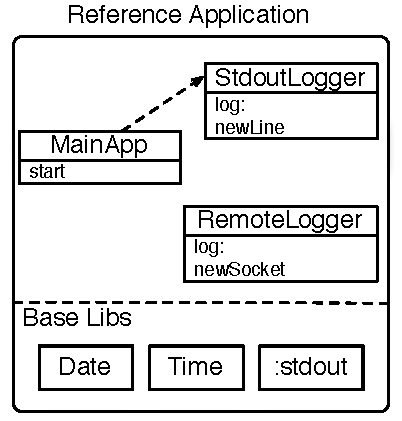
\includegraphics[width=.5\linewidth]{example_reference}
\caption{\small\textbf{Reference application with all code units.}\label{fig:example_reference}}
\end{center}
\end{figure}


\begin{figure*}[ht]
\begin{center}
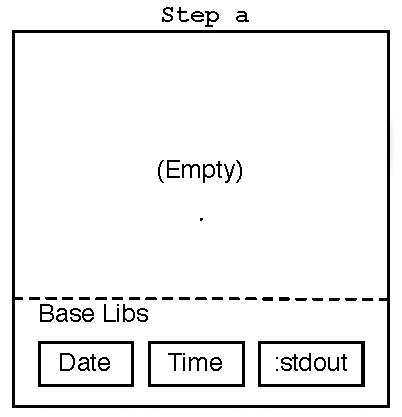
\includegraphics[width=.322\linewidth]{example_before}
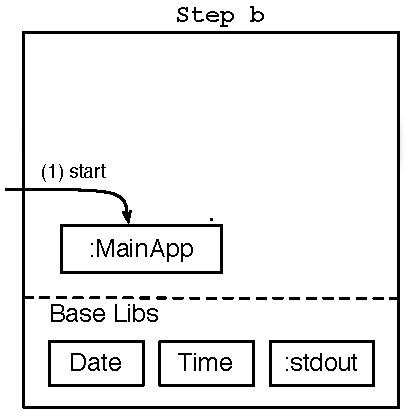
\includegraphics[width=.33\linewidth]{example_starting_point}
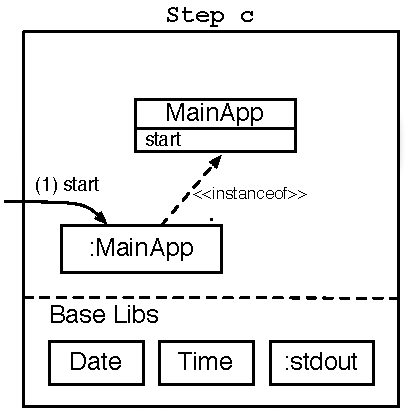
\includegraphics[width=.33\linewidth]{example_dnu_trap_start}
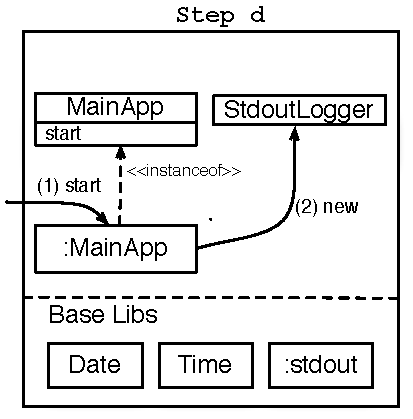
\includegraphics[width=.33\linewidth]{example_shadow_trap}
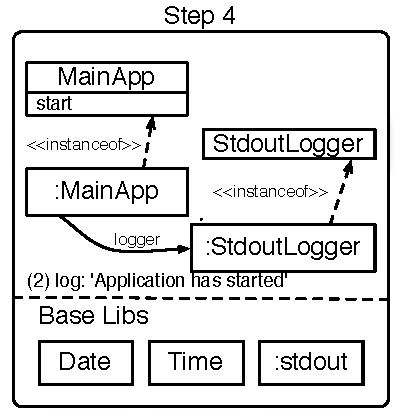
\includegraphics[width=.325\linewidth]{example_dnu_trap}
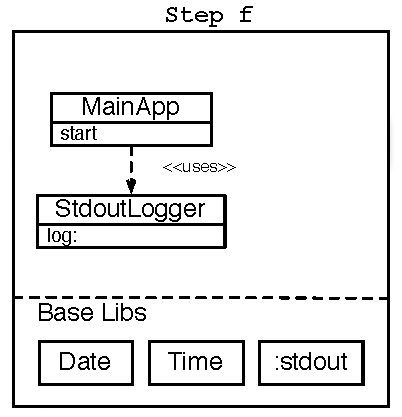
\includegraphics[width=.33\linewidth]{example_finished}
\caption{\small\textbf{The nurtured application at different steps of tailoring.} \label{fig:example_all}}
\end{center}
\end{figure*}

\paragraph{Install the application's entry point} We install into the nurtured application our application's entry point \ie a \ct{MainApp} instance~(\ct{aMainApp}) and a process that will execute the statement \ct{"aMainApp start"}~(cf. Figure~\ref{fig:example_all} Step b). Note that although we are referencing an instance of the class \ct{MainApp}, the \ct{MainApp} class is not installed yet.

%\begin{figure}[ht]
%\begin{center}
%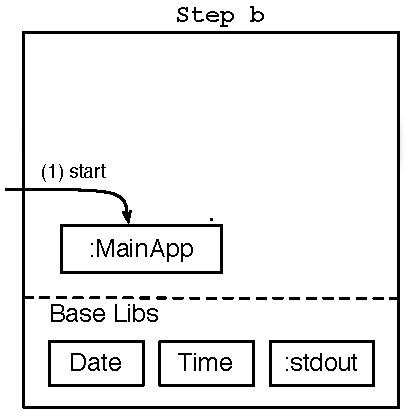
\includegraphics[width=.8\linewidth]{example_starting_point}
%\caption{\textbf{Installing an entry point.} The nurturer installs the entry point of the application and starts its execution sending it the \ct{start} message.\label{fig:example_starting_point}}
%\end{center}
%\end{figure}

When the execution starts, the \ct{mainApp} instance receives the \ct{start} message, and we detect the \ct{MainApp} class and its \ct{start} method as a missing code unit failure. We install these two missing code units~(cf. Figure~\ref{fig:example_all} Step c) and finally the \ct{MainApp>>start} method is activated and starts running.

%\begin{figure}[ht]
%\begin{center}
%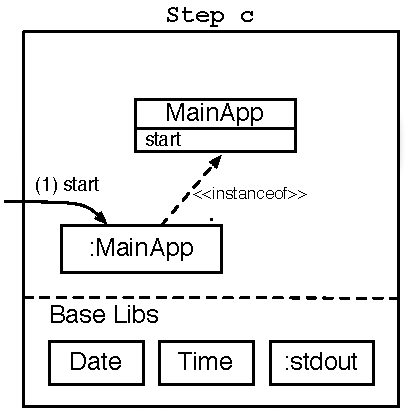
\includegraphics[width=.8\linewidth]{example_dnu_trap_start}
%\caption{\textbf{Activating the entry point.} The nurturer installs the \ct{MainApp} class and the \ct{start} method on demand.\label{fig:example_dnu_trap_start}}
%\end{center}
%\end{figure}

\paragraph{Activating the start method}
The method \ct{start} defined in Figure~\ref{fig:code_example_again} is executed, as we can see in Figure~\ref{fig:example_all} Step c. During the execution of its first statement~(Figure~\ref{fig:code_example_again} line 2) we detect a missing code unit failure: The \ct{StdoutLogger} class does not exist. Thus, before continuing, we install a \ct{StdoutLogger} class with the same shape as its reference counterpart~(cf. Figure~\ref{fig:example_all} Step d). This class does not contain, however, all the methods nor the meta-data (\eg superclass, package, subclasses) from the reference class since they may not be necessary.

%a \emph{shadow} of the \ct{Formatter} class~(Figure~\ref{fig:example_shadow}).\gp{I don't like the word shadow here, since it does not go with the tailor metaphor} The \ct{Formatter} shadow is a proxy object the tailor will use to know if and when the \ct{Formatter} class is used.

%\begin{figure}[ht]
%\begin{center}
%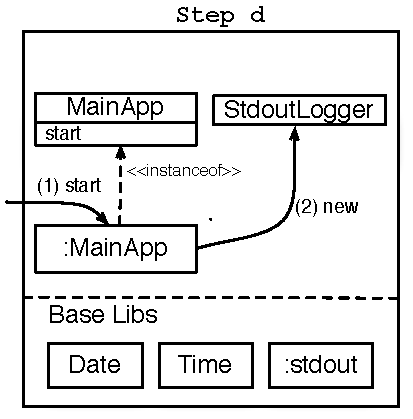
\includegraphics[width=.8\linewidth]{example_shadow_trap}
%\caption{\textbf{Activating the \ct{new} method.} The nurturer installs a the \ct{StdoutLogger} class and sends it the \ct{new} message.\label{fig:example_shadow_trap}}
%\end{center}
%\end{figure}

%Once the \ct{Formatter} shadow is available, the tailor can continue the execution and send the message \ct{new} to the shadow object. At this point, the tailor finds out that the receiver of the \ct{new} message is a shadow object, and thus, it replaces the shadow object by

%Note that copies of classes are treated specially: they contain a method dictionary where methods are installed, but since no instance of \ct{Formatter} received yet a message, its method dictionary is empty.

Once we install the \ct{StdoutLogger} class, we resume the execution. The first statement results into a new \ct{StdoutLogger} instance. Note that the \ct{new} method is already installed because it is part of the language base library, already available in the seed. 
During the second statement's execution~(Figure~\ref{fig:code_example_again} line 3), we detect a missing code unit failure on the \ct{log:} message~(cf. Figure~\ref{fig:example_all} Step e): the corresponding method is not installed in the \ct{StdoutLogger} class. We install it and resume the execution. This time the method is found, and the \ct{log:} method is activated.

%\begin{figure*}[ht]
%\begin{center}
%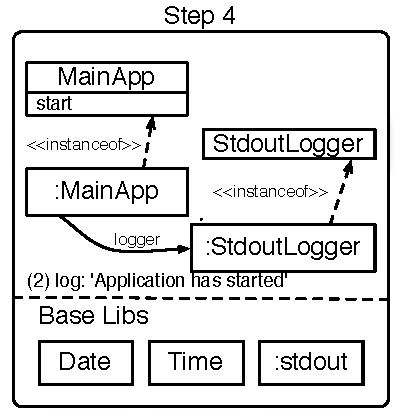
\includegraphics[width=0.65\linewidth]{example_dnu_trap}
%\caption{\textbf{Activating the \ct{log:} method.} The message \ct{log: 'Application has started'} is sent to the \ct{logger} object. \label{fig:example_dnu_trap}}
%\end{center}
%\end{figure*}


Once the \ct{log:} method finishes, the execution returns to the \ct{start} method. There, the third statement~(Figure~\ref{fig:code_example_again} line 5) is executed with no intervention of our technique, since the \ct{log:} method is already available. Figure~\ref{fig:example_all} Step f shows the final state of the nurtured application: it contains only the methods and classes that are actually used by the application. Leaf objects used during the process have been garbage collected.

%\begin{figure}[ht]
%\begin{center}
%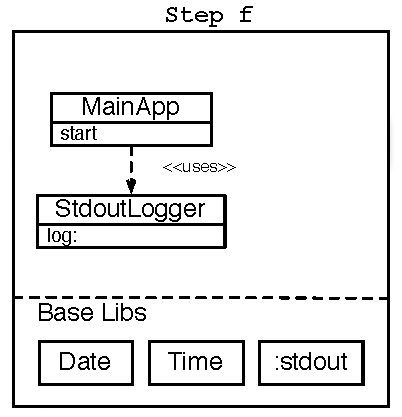
\includegraphics[width=.8\linewidth]{example_finished}
%\caption{\textbf{Final state of the nurtured application.} The nurturing has finished and the resulting application is tailored.\label{fig:example_finished}}
%\end{center}
%\end{figure}

\section{Detecting Missing Code Units}\label{sec:model_detail}

RFG depends on getting notified when a missing code unit failure appears. RFG's algorithm is based on traps to achieve this task, as shown in Algorithm~\ref{alg:tailoring_process}. Traps are placeholders that are installed in the nurtured application in the place of real elements. They are triggered whenever the application tries to access them. In case a trap is triggered, we suspend the nurtured application execution, we install the missing code units replacing their corresponding traps, and finally resume the execution from the moment immediately before the trap was triggered. Traps are installed dynamically in the nurtured application following the information flow of the application \eg when a method \ct{A} is installed some traps are installed inside it to capture possible missing code unit failures it may cause.

\begin{algorithm}[ht]
 %\KwData{this text}
 %\KwResult{how to write algorithm with \LaTeX2e }
 Initialize reference application\;
 Initialize nurturing application with the seed\;
 Install entry point(s)\;
 \While{not finished}{
  run the nurtured application\;
  \If{trap was activated}{
   install missing code units\;
   restart message send;
  }
 }
 \caption{\textbf{An abstract view of the run-fail-grow process.}\label{alg:tailoring_process}}
\end{algorithm}

RFG follows the next rules to install code units inside the nurtured application:

\begin{enumerate}
\item Classes are installed when we install a method that belongs to them or one of their superclasses.
\item Methods are installed when they need to be executed, following the rules of the method-lookup in the underlying \VM.
\item Objects are installed when a message is sent to them, including self and super sends.
\item Objects are installed when they are needed by the \VM to execute some operation~(\eg primitives and method literals).
\end{enumerate}

Then, we identify the following as the basic traps that are necessary to tailor an application.

\begin{description}
\item[Missing object trap.] A \emph{missing object} trap captures messages sent to objects that do not yet exist inside the nurtured application such as classes. When RFG finds one of these traps, its responsibility is to install the corresponding object. The object installed is a \emph{partial} clone of the original object \ie not all of its state is installed, instead it contains traps to capture the access to its class and fields. When a method refers to a static variable, we install one of this traps for it.

\item[Missing method trap.] A \emph{missing method} trap captures me\-thod invocations whose methods are not defined in the nurtured application yet. When the application execution triggers one of these traps, RFG installs the corresponding method in the class hierarchy of the object. In the class that will own the method does not exist, RFG will install it too. Method literals (\eg strings and numbers that are part of the method definition) are installed along with the method that owns them because the \VM can manipulate them directly during the bytecode interpretation.

\item[Missing override traps.] A particular case of missing method traps are \emph{missing override traps}. A missing override trap captures overridden methods. This avoids that the method lookup answers a superclass implementation resulting into an unexpected behavior. Figure~\ref{fig:need_override} illustrates this problem: the class \ct{B} from the reference application contains an override, while it is not present in the nurtured application. If no trap is placed to capture the override, the method \ct{doSomething} from class \ct{A} would be executed, thus changing the semantics of our application.

\end{description}

Note that there is no need for a \emph{missing class trap} as classes are installed when a \emph{missing method trap} is triggered. In the case of languages that expose classes as objects, classes can also be installed by missing object traps when we send a message to them.


\begin{figure}[ht]
\begin{center}
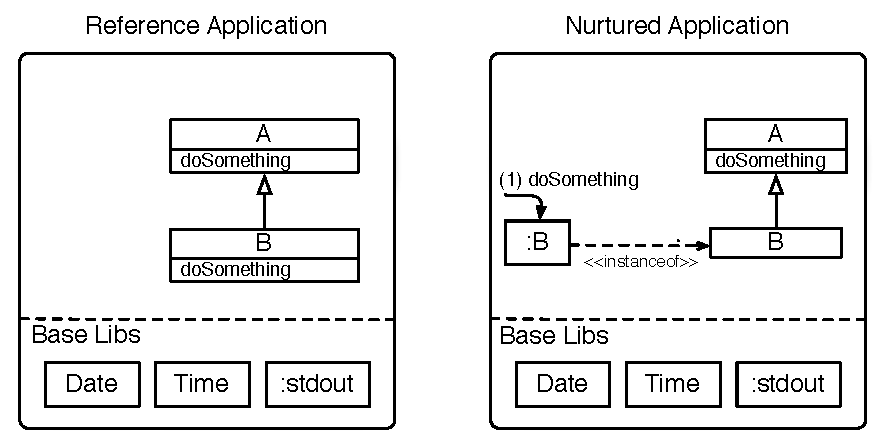
\includegraphics[width=0.7\linewidth]{need_override}
\caption{\small\textbf{The need of overriding traps.} \small Method traps should capture the overridden \ct{doSomething} message-send to avoid the superclass method to be executed wrongly.\label{fig:need_override}}
\end{center}
\end{figure}



\section{Customizing Dead Code Elimination with Seeds}\label{sec:seeds}

The level of tailoring of RFG can be specified using seeds. A seed is a collection of code units whose installation is forced into the nurtured application. These code units are available for the nurtured application and thus, accessing them does not trigger missing code unit failures. A seed can contain any arbitrary code unit, including package, classes, methods and even already initialized objects. Seeds are useful to cover different tailoring scenarios.

Let's take as a first example a smartphone where the base libraries of the language are already available, so they are shared amongst the many applications installed in it. When targeting such a smartphone, base libraries are already present and we do not need to produce a specialized version of them. We need to specialize only third-party libraries and application code. In this case, we use a seed providing the language base libraries.

Let's take as a second example a constrained device robot-like which will contain only our application. When targeting this robot as deployment scenario, we want to specialize all the code to deploy including base libraries. In such a case, the seed is empty to allow the RFG algorithm to work on every code unit.

Figure \ref{fig:nurturing_map_model} presents two tailoring maps showing exemplar usages of seeds. Each application contains code units corresponding to the base libraries, third-party libraries and application code. To the left the seed covers base and third party libraries, thus RFG applies and selects a subset of the application code units only. To the right, the seed covers only the base libraries, thus RFG applies and select a subset of the code units from the third party libraries and application code.

\begin{figure}[ht]
\begin{center}
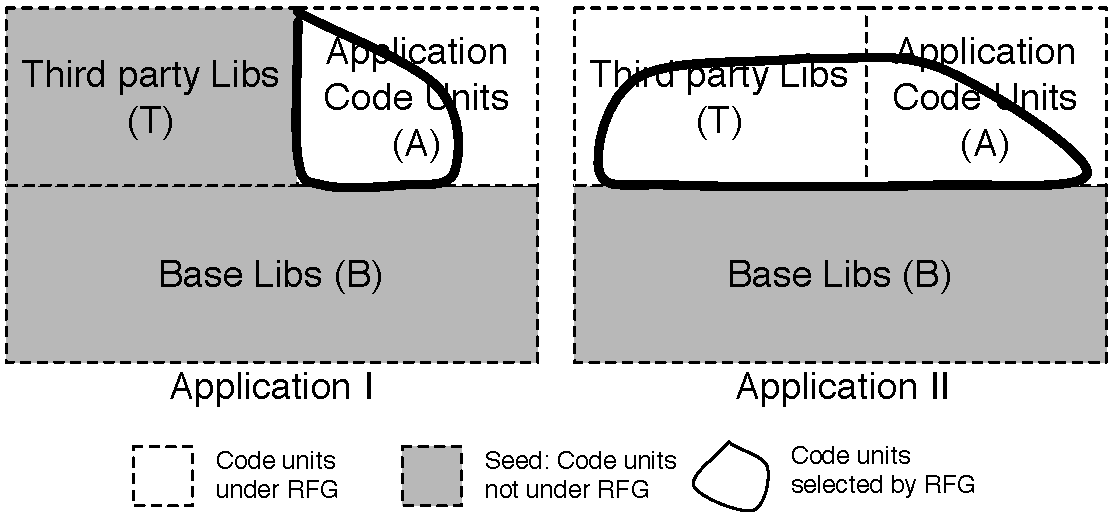
\includegraphics[width=.7\linewidth]{nurture_map}
\caption{\small\textbf{Tailoring Map.} A tailoring map describes which code units of an application are included in the seed~(in gray), which ones are subject to the RFG technique~(in white) and the amount of them that are finally selected~(within the thick area).
\label{fig:nurturing_map_model}}
\end{center}
\end{figure}


%============================================================================
\section{Tornado: RFG in \Vtt} \label{sec:rfg_implementation}

We implemented our RFG technique as a tool called \emph{Tornado}. Tornado is implemented using \Vtt, to tailor applications written in the Pharo programming language.
%Pharo is a reflective and dynamic programming language inspired from Smalltalk.
Tornado's architecture combines \Vtt~(cf. \chapref{vtt}) and Ghost proxies~(cf. Section \ref{sec:proxies}) illustrated in Figure \ref{fig:tornado_code units}. The nurtured application is hosted inside an object space  Tornado's hypervisor runs and monitors the nurtured application. It installs traps on the nurtured application as Ghost proxies, and use the object space interface to query and install code units it. Following, we detail how we fulfilled each of RFG's requirements in our solution:

\begin{figure}[ht]
\begin{center}
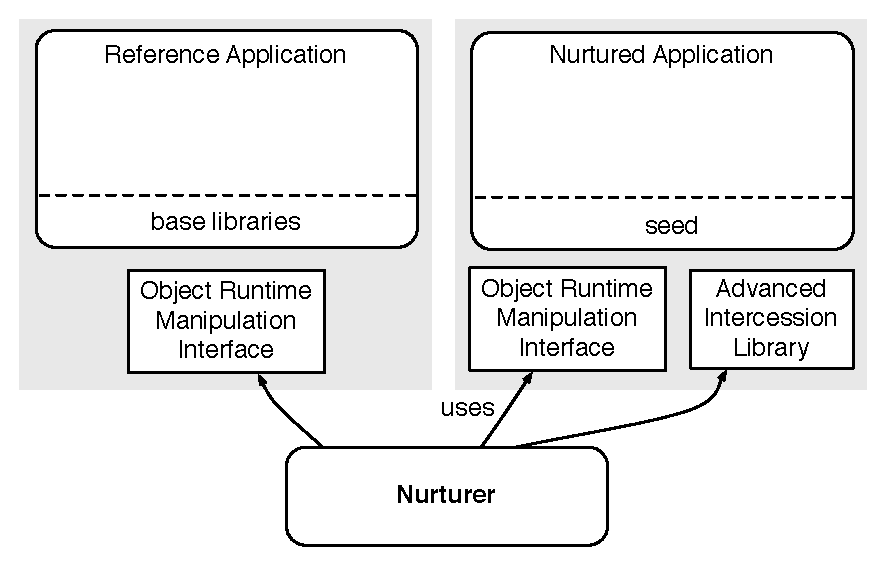
\includegraphics[width=0.8\linewidth]{tornado_components2}
\caption{\small\textbf{Tornado's architecture overview.} Tornado controls both the reference and nurtured applications through Espell. Traps are installed into the nurtured application with the Ghost library.\label{fig:tornado_code units}}
\end{center}
\end{figure}

\begin{description}
\item[Execution cycles.] We use \Vtt execution cycles to monitor and control the execution of a nurtured application. When a cycle is finished the Tornado hypervisor checks if the virtualized runtime is suspended on a trap. In such case, it installs the corresponding code unit and resumes the execution with another cycle.

\item[Advanced proxies.] Pharo's libraries includes Ghost~\cite{Mart11a}, an advanced proxy implementation. Ghost allows one to capture all kind of message sends, intercept particular method executions, and even to proxy classes and special objects. We use the Ghost model to implement execution traps.

\item[Object space runtime manipulation.] An object space provide already with operations to query and install the classes and methods in the virtualized runtime.

\end{description}

\subsection{Execution Traps with Ghost Proxies} \label{sec:proxies}

Implementing execution traps such as the ones described in Section~\ref{sec:model_detail} requires powerful intercession support. Traps must capture \emph{all} message sends to objects provided by the application runtime as well as the application objects, including classes~(for example for the case of class messages or static methods). They must capture \emph{self} and \emph{super} message sends, as well as overrides and particular method invocations.

To achieve this, we implemented a set of proxies following the Ghost model~\cite{Mart11a}~(similar to JavaScript proxies~\cite{Vanc10a}). Ghost proposes a low-memory footprint, general purpose proxy implementation for the Smalltalk language supporting the creation of proxies for normal objects as well as classes and methods. 
% These proxies allow the interception of all message sends.
% When a Ghost proxy captures an invocation, it triggers the behavior of a \emph{handler}. 
% The Ghost proxy library provides already several kinds of handlers including for example message forwarding or logging.
Using Ghost proxies we are able to detect all situations corresponding to our traps.
Ghost proxies represent missing objects, classes and methods. When a proxy is accessed, Tornado replaces it by its corresponding real object.
Tornado correctly respect identity by using a table relating each proxy to the code unit or object it represents in the reference application.
%Ghost proxies capture all messages.
Additionally, each proxy is attached to a \emph{handler} that may perform some action when the proxy receives a message.
We use proxy handlers to perform the right action for each trap.
We discuss below the different kinds of proxies and handlers we use and how they support RFG.

\begin{description}
\item[Missing object trap.] This trap is implemented as a proxy taking the place of a normal object. This trap is triggered when the proxy receives a message.
Its handler replaces the proxy by a \emph{partial} copy of the original object from the reference application.
The copy is created, and all references to the proxy are replaced by references to this new object, which is achieved through the \ct{become:} facility of the Pharo language that dynamically swaps object references.
Each field and the class of this new installed object are installed as new missing object traps.

\item[Missing method trap.]  We implemented the missing method trap in Tornado as a class proxy located at the top of the class hierarchy. Whenever a message is sent to an object, the VM looks up the method in the object's class hierarchy. This trap is triggered whether a message arrives to the top of the hierarchy, meaning that there was no method for it in the hierarchy. When triggered, the handler installs the classes part of the hierarchy of this method and the missing method in its corresponding class. If no method is found to install, Tornado sends the \ct{doesNotUnderstand:} message~(an equivalent to \eg Ruby's \ct{method\_missing} and Python's \ct{\_\_getattr\_\_}) to honor the dynamic semantics of Pharo.

\item[Missing override trap.] We implemented missing override traps in Tornado using method proxies. Method proxies are placed in the method dictionaries of classes containing overriden methods, taking the place of the original method.  When Tornado installs a class into the nurtured application that contains overridden methods in the reference object space, it installs into this class a method proxy for each of its overridden methods. This trap is triggered whenever the method proxy it is about to be executed. The handler of this trap compiles a new method with the same source as the corresponding method from the reference application and installs it inside the nurtured object space.

\item[Primitive methods trap.] Primitive method traps are implementation specific related to the Pharo language. Pharo's primitive operations such as number arithmetic are implemented through primitive methods. Primitive methods are implemented in the Virtual Machine and do often access directly the fields of its receiver and arguments by forging references and manipulating directly the memory, bypassing our traps. Thus, we face an issue when a \emph{missing object trap} proxy is the argument of such a method: the VM can modify this proxy without activating the trap. Primitive method traps are method proxies that decorate Pharo's primitive methods. When they are triggered because one of these methods is about to be executed this trap's handler triggers each of the missing object traps received as arguments, if any. In this way, Tornado forces the installation of the arguments and the primitive is executed with actual objects instead of proxies, as expected.

\end{description}

% \subsection{Traps and Proxies}\label{sec:traps}
% Tornado traps notify the nurturer when some object is missing. In such case, the tailor installs the missing object and continues the execution from the point where it was trapped. Traps are implemented in Tornado through Ghost like proxies. Each trap in tornado is a Ghost proxy. Tornado implements a custom interception handler: every time a trap is activated, the object space where the trap is located gets paused and the control is returned to the tailor to treat the trap. Following, we explain each of the traps implementations and how they are treated by the tailor:
% 
% \begin{description}
% \item[Not-installed trap.] A trap for an object or class not yet installed in the system is a simple proxy. If the proxy receives a message, the tailor installs the object the proxy represents and replaces the proxy by the new object. If the new object has fields, these fields will be propagated as proxies or installed depending on its particular mapping~(cf. section~\ref{sec:mappings}). In our particular implementation, the replacement of the proxy by its new counterpart is done through the \ct{become:} facility of the Pharo language that allows pointer swapping.
% \item[Does not understand trap.] We implemented the does not understand trap in tornado as a class proxy situated on the top of the class hierarchy. Whenever a message is sent to an object, the method lookup mechanism searches a method with the same firm in the object's class hierarchy, starting from the object's class up to the top. Our does not understand trap captures whether a message arrives to the top of the hierarchy, meaning that there was no method for it in the hierarchy. When this trap is activated, the tailor looks in the model application for the method to install, installs it in the nurtured application and finally restarts the execution from the call-site that activated the trap.
% 
% \item[Override trap.] We implemented override traps in tornado using method proxies. Method proxies are activated whenever the proxified method is about to be executed. When Tornado installs a class that contains overridden methods in the reference object space, it also installs into it one method proxy for each of its overridden methods. In such a way, the method lookup mechanism finds the overridden traps and returns the control to the tailor. In turn, the tailor installs the method corresponding to the trap and restarts the execution from the call-site that activated the trap.
% 
% \item[Primitive methods trap.] \gp{il faut l'ecrire}
% 
% \end{description}
% 
% \gp{Traps are placed in the tailoring application so they get activated only when the special cases are given. They do not represent a penalty on runtime during the tailoring process.}
% 
% Note that every time a trap is captured and treated, restarting the execution must handle correctly self and super message-sends\footnote{A super message-send starts the method lookup from the superclass of the class where the actual method in execution is located, instead of the class of the message receiver}. Thus, Tornado always restarts the execution respecting the call-site and the class where the method lookup mechanism started to maintain the program's semantics, regardless the kind of trap that was activated.


\subsection{Object Installation and Propagation Rules} \label{sec:mappings}

As we explained before, Tornado installs all objects inside the nurtured application on demand, as \emph{partial copies}, \ie the objects referenced by the original object will not be copied along with it by default, but traps are placed instead of them. %That is, no object, class or method is installed unless it is needed by the application to run. The need for installing some element is detected by means of traps~(cf. Section~\ref{sec:model_detail}).
%The tailored application contains during the tailored process two kind of objects: application objects that are copies of the model application objects, and proxy objects representing traps.
When Tornado installs an object inside the nurtured application, this new object has the same format and size as its original counterpart. \emph{Propagation rules} determine how each of the object's fields are propagated on installation. Tornado provides the following propagation rules to customize installation:

\begin{description}
\item[Missing object trap.] This is the \emph{default propagation rule} and end user applications can usually be tailored with just them. This propagation rule installs a missing object trap in each field of the object that is being installed.
\item[Materialization.] This propagation rule forces the installation of the object referenced by the field. This is used for those cases where some structure should be guaranteed to the Virtual Machine \eg the objects referenced by the first three fields of a class~(superclass, format and method dictionary) cannot be proxified because they are used by the VM for the method lookup. The same happens with other objects reifying low level concepts such as activation records or semaphores.
\item[Swapping.] This propagation rule forces the reference of the object installed be swapped to another object's reference. The usual use case of this rule is replacing some object reference by \ct{nil}, and so, to force lazy initializations.
\end{description}

% Figure \ref{fig:character_mapping} shows an example of the mapping of the \ct{Character} class which forces the materialization of the character and digit tables class variables.
%
%\begin{figure}[ht]
%\small
%\begin{code}
%Character >> tornadoMappingFor: aTornado
%	^ (super tornadoMappingFor: aTornado)
%			mapClassPoolWith: { 
%				#CharacterTable -> ToMaterializationPropagationStrategy new.
%				#DigitValues -> ToMaterializationPropagationStrategy new
%			}; yourself
%\end{code}
%\caption{\small\textbf{Mapping for class \ct{Character}.} Mapping forcing the installation of the character and digit tables needed by the VM. \label{fig:character_mapping}}
%\end{figure}

\subsection{Object Identity and Proxies}

Tornado takes care of the identity of objects with an identity table. The identity table is important because Tornado works at the object granularity. Due to the inherent graph nature of object-oriented programs, an object being installed may reference another object that is already installed inside the nurtured application.
Identity is an important concern in the presence of proxies. Tornado guarantees that identity checks inside a program~(\eg comparison through \ct{==}) always preserve object identity by following the following invariant: 

\begin{center}\emph{An object and its proxy do not exist concurrently in the nurtured application.}\end{center}

That is, the nurtured application contains either an object, either the proxy trap that represents its absence, but not both at the same point in time. When the proxy is replaced by the actual object's copy, all references to the proxy are swapped to references to the new object. The proxy is no longer referenced and thus, garbage collected. This invariant guarantees that identity checks in a program that should be \ct{true} are indeed be \ct{true}. Either the compared references point both to the same proxy, or both to the same \emph{partial} copy.

\subsection{Implementing Seeds in Tornado}

Tornado's seeds specify the level of tailoring. The seeds are in charge of initializing the nurtured application's virtualized runtime with the elements we want to ensure on it. Our current prototype supports two ways of describing and building seeds: 

\begin{description}
\item[Loading an already existing memory snapshot.] The nurtured application's object space is initialized by loading an already existing snapshot or image~(\ie this is an image in the same sense as Smalltalk or Lisp). This technique consists in using a memory dump from an object heap containing all the classes and objects desired in the seed. This memory snapshot should follow Pharo's object format. 
\item[Creating all seed code units from scratch.] The nurtured application's object space is initialized with objects built from scratch. This technique uses a bootstrapping process as described in \chapref{bootstrapping}.
\end{description}

%Note that a seed can indeed contain any arbitrary code units and objects. They are not restricted to have only base or third party libraries. The selection or extraction of what is included as part of a seed is application dependent and orthogonal to the run-fail-grow process. We show an example of it in Section \ref{sec:results}.

\subsection{Preparing the Application for Deployment}\label{sec:deploy}

Once Tornado is stopped, the nurtured application contains all the code units needed to run. Tornado procceeds to prepare the application for deployment \ie it removes all trap leftovers and extracts the nurtured application. Tornado identifies the traps by the presence of proxies and replaces the references to those proxies by references to another object, defaulting to the \ct{nil} object. Proxy objects do not then represent a drawback in space consumption because they are garbage collected. Once the traps are removed, the nurtured application keeps no dependencies to Tornado nor its infrastructure. Thus, the application can run outside the Espell infrastructure with no performance penalties.

Finally, Tornado extracts the application code units using one of two different techniques: (a) the creation of a snapshot file containing all code units and already initialized objects; or (b) build a static description of the application containing the code for all classes and methods that should be part of it.

\section{Conclusion and Summary}

In this chapter we presented a run-fail-grow~(RFG) approach for application tailoring. RFG tailors an application by starting it and initializing it with a seed that contains the minimal set of code units we want to ensure. Then, we install and execute the application's entry points. As the application executes, missing code units are found and installed on demand, ensuring that only the needed code units are introduced. By following the runtime execution, it supports dynamic features such as reflection and meta-programming.

We implemented RFG in a tool called Tornado based in \Vtt. With \Vtt, we are able to monitor the nurtured application's execution using the execution cycles. Mirrors allows us to easily install required code and restart the execution as it is needed.

\chapter{Validation}
\minitoc
\introduction

%\section{Experiments and Results}\label{sec:results}
%
%\subsection{Experiment's Methodology}
We evaluate Tornado by conducting five experiments that tailor different Pharo applications, with increasing requirements~(Section \ref{sec:rfg_experiments}). We chose our experiments under the objectives of (a) understand how minimal are the applications we can tailor, (b) explore how successfully we address the challenges we stated in Section \ref{sec:challenges} and (c) exercise those cases that push to the limit the interaction between the language and the VM. Our experiment methodology consists in the following steps:

\begin{enumerate}
\item \textbf{Setting up a seed for the application.} Most of our experiments use what we already called an \emph{empty seed}. This seed is, however, not completely empty. The empty seed we used contains some minimal infrastructural objects that are needed for language-VM interaction, and is therefore 10KB large. Our last experiment, the largest one, uses both this empty seed and an additional seed containing the base libraries. 
\item \textbf{Preparing the application entry points.} This step consists in the installation of the one or more processes that will run our application.
\item \textbf{Run the application.} The application is run, its threads executed. In particular in our last experiment~(an interactive web application), we interact with our application through a web browser. 
\item \textbf{Stop and extract the application.} Once the tailoring process finishes, we stop Tornado and extract the resulting application by making a snapshot of it in a Pharo image file. We test the generated snapshots to verify they work properly, either by using the application or debugging them when they involve no I/O. We evaluate the behavior of the tailored application under the assumption that only the features we used during the tailoring should work.
\item \textbf{Perform measurements.} Finally, we measure the size of the generated snapshots files and compare them against two different Pharo distributions prepared for production~(cf. Section \ref{sec:results_discussion}).
\end{enumerate}

Additionally, we present an evaluation of Tornado according to the evaluation criteria stated in \chapref{state_virtualization}. Our evaluation includes a comparison with the already presented related work on application tailoring~(Section~\ref{sec:rfg_evaluation}).
Finally, we discuss some aspects and trade-offs of the run-fail-grow approach and our implementation~(Section~\ref{sec:discussion}).

\section{Experiments}\label{sec:rfg_experiments}

\subsection*{Experiment I: Adding Two Numbers}

The smallest~(in terms of size) interesting program to tailor is adding two numbers, without the involvement of any I/O \ie an application just executing the \ct{"2 + 3"} statement as entry point. Tailoring this program is challenging because it stresses the infrastructure by installing only the minimal elements an application needs to run. It makes evident how small a tailored application can be. Additionally, it is interesting since it makes use of the following features of the Pharo language and infrastructure:

\begin{description}
\item[Immediate objects.] Immediate objects are objects encoded in the object reference instead of being allocated in the heap. Immediate objects do not contain a reference to their class in the object header, as there is no object header. Instead, the object reference where the object is encoded contains a bit tag that the VM uses to identify the immediate object. This means that the Pharo VM must acknowledge the immediate object classes~(or their proxies) in order to send messages to these immediate objects. In this experiment we use immediate small integers, instances of \ct{SmallInteger}.
\item[Special selectors.] The method selector \ct{+} is a special selector for the Pharo VM. Special selectors are optimized as they are broadly used messages, for example for arithmetics. First, they are implemented as special bytecodes to avoid method lookup. If the special bytecode cannot be executed because some VM assertions are not valid~(\eg class and object format assumptions), the VM performs the default method lookup. In this experiment the VM should take care of small integer arithmetic \ie it should fulfill all VM assumptions and not perform a method lookup; Tornado should install no extra methods nor classes.
\end{description}

\subsection*{Experiment II: Factorial of a little number}

The following experiment in incremental complexity is the factorial of a small number, again without the involvement of any I/O \ie an application executing the \ct{"10 factorial"} statement as its entry point. Factorial uses arithmetic as the latter experiment~(sums and multiplications), while it also adds the following interesting cases:

\begin{description}
\item[Method lookup.] The \ct{factorial} message is sent to a small integer but not optimized as it is not a special selector. Thus, the VM look ups the corresponding method up in its class hierarchy. The method \ct{factorial} is defined in its superclass~(\ct{Integer}).
\item[Recursion.] The factorial implementation in Pharo base libraries is recursive. Additionally, this recursion activates the \ct{factorial} method many times, creating many activation records in the VM. Activation records are reified lazily whenever it is accessed reflectively, or the stack depth is deeper than the maximum supported.
\end{description}

\subsection*{Experiment III: Factorial of a large number}

Following, we experimented with an application whose entry point was the \ct{"100 factorial"} statement. This application does not either make use of any I/O. The factorial of a large integer creates eventually integers that exceed 32 bits, and thus, do not fit as immediate small integers. This experiment adds the following interesting cases:
\begin{description}
\item[Large integers.] Large integers in Pharo are represented, in contrast to immediate small integers, as objects allocated in the heap with their own object header and arbitrary length. Large integers are created automatically by the VM when the result of some integer calculation produces a number that overflows 31 bits. That is, the LargeInteger class (or its proxy) should be available to the VM in order to instantiate the correct object.  Additionally, large integers implement their arithmetic methods by calling primitives from external plugins~(the large integers plugin).
\item[Polymorphism.] The introduction of large integers introduces also \emph{polymorphism} between them and the immediate small integers. They share the same class hierarchy~(\ct{Integer} is the superclass of \ct{SmallInteger} and \ct{LargePositiveInteger}), being the method \ct{factorial} implemented in the superclass and having each of the subclasses their own implementation of the arithmetic methods for adding and multiplying.
\end{description}

\subsection*{Experiment IV: Reflective invocations} \label{sec:results_helloworld}

The fourth experiment introduces reflective invocations. Figure \ref{fig:reflective_invocations} introduces the code we used for this experiment. The \ct{User} class in our example has two fields (\ct{name} and \ct{age}), and four methods. Two of these methods (\ct{age} and \ct{name}) return directly the field with the same name, the method \ct{hasWritePermissions} is annotated with the \ct{property} annotation (a pragma in Pharo's terminology) and the method \ct{isMinor} is a normal method. We introduce also \ct{PropertyExtractor} class with the responsibility of returning the name of those methods that are properties of an object \ie all methods that only return a field, and all those methods annotated with the \ct{property} annotation. The statement we introduced as the entry point for this experiment is \ct{"PropertyExtractor new extractPropertiesFrom: User new"}.

\begin{figure}[ht]
\small
\begin{code}
Object subclass: #User
	instanceVariableNames: 'name age'.

User>>age
	^ age

User>>hasWritePermissions
	<property>
	^ true

User>>name
	^ name

PropertyExtractor>>extractPropertiesFrom: anObject
	^ anObject class methods
		select: [ :each | each isReturnField
			or: [ each pragmas anySatisfy: [ :pragma | pragma keyword = #property ] ] ]
		thenCollect: [ :each | each selector ]

\end{code}
\caption{\small \textbf{Code of the reflective invocations experiment.} The \ct{PropertyExtractor} class does the reflective invocations, the \ct{User} is the class we will be reflecting on.\label{fig:reflective_invocations}}
\end{figure}

This experiment evaluates how do we handle the reflective abilities of Tornado's RFG. The \ct{PropertyExtractor} queries the methods from the \ct{User} class, that are included as part of the tailored application~(since they receive the messages \ct{isReturnField} and \ct{pragmas}). These reflective invocations include: (a) access to an object's class, (b) access class methods and (c) query those methods to know if they correspond to the criteria of the \ct{PropertyExtractor}.

\subsection*{Experiment V: Adding I/O} \label{sec:results_helloworld}

A fifth experiment introduces I/O to each of the previous experiments, adding a statement printing to the standard output the obtained results. Figure~\ref{fig:hello_world_entry_point} shows the code from our entry point in the case of summing up two numbers. The entry points for the other experiments have the same structure, differing only on the expression that is printed~(the \ct{"1+2"} expression in this case). Notice that the \ct{FileStream} class needs to be initialized before the proper printing into the stdout stream because the code needed for class initialization is not installed by default in the empty seed.

\begin{figure}[ht]
\small
\begin{code}
FileStream startUp: true.
FileStream stdout 
	nextPutAll: (1 + 2) asString;
	crlf.
\end{code}
\caption{\small \textbf{Entry point of the experiment that sums two numbers and prints the result in the standard output stream.}\label{fig:hello_world_entry_point}}
\end{figure}

In this experiment, besides testing the proper usage of I/O streams such as the standard output stream, we evaluate the ability of Tornado to handle \textbf{platform identification}. The \ct{stdout} stream initialization for Pharo is done by the File package written in Pharo, and it depends on which is the current operating system. This experiment shows that Tornado prepares tailored versions of applications to run on a single operating system or platform.

\subsection*{Experiment VI: Seaside Web Application}



Our last experiment consists is tailoring a web application using Seaside application framework~\cite{Duca07a}. Seaside is a web application framework featuring continuations thanks to stack reification. We configured it with its default values, without making any customizations. The web application under tailoring has a single webpage that allows one to send requests to the web server to increase or decrease a counter. This experience shows that Tornado works in presence of \textbf{threading}. The Seaside application framework makes use of Pharo processes. One process listens incoming connections and opens new processes to handle requests. Seaside uses semaphores to synchronize processes and wait for incoming data from sockets.

For this case, we proceeded to do two different experiences, with two different seeds. We first used the empty seed~(\emph{Seaside Web Application A}), as in the previous experiments, and then used a seed containing all Pharo base libraries~(\emph{Seaside Web Application B}). For reasons of space, the details of how the entry points are initialized for these both seeds can be found in our technical report~\cite{Poli14a}.

\section{Results} \label{sec:results_discussion}

We gathered our experiments' results into Table \ref{tb:results}. This table shows:
\begin{description}
\item[Experiment.] The name of the experiment under evaluation, followed by our measurements.
\item[Reference Application.] The size of the reference application containing all of its code units, in KB. We present in here two different sizes: the size of an experimental shrunk version of the Pharo distribution called \emph{PharoKernel}, which was developed independently from us by Pavel Krivanek; and between parenthesis the size of the official Pharo distribution prepared for production: Pharo allows one to prepare a snapshot for production. This option cleans some caches and removes some well known objects and classes from the system, thus, freeing space.
\item[Seed.] The size in KB of the chosen seed for the experiment.
\item[Nurtured Application.] The final size of the nurtured application once Tornado finishes its process and the application is extracted.
\item[Saved.] The percentage of space saved using the smallest reference application size. We chose the smallest reference application to avoid biased results in our favor. We calculated this percentage using the following equation:

\begin{equation*}
saved = 100 - \frac{100*(nurtured - seed)}{reference - seed}
\end{equation*}

\begin{table}[ht]
 	\centering
 	\begin{tabular}{lccccc}
		\toprule
			Experiment
 			& \textbf{Reference App}
			& \textbf{Seed}
			& \textbf{Nurtured}
			& \textbf{Installed}
			& \textbf{Saved(\%)}\\
			
 			& \textbf{\emph{Shrunk(Prod.)}}
			& \textbf{Size}
			& \textbf{App}
			& \textbf{Code}
			& \textbf{}\\
		\toprule
		Sum Two
 			&  3799 (12873) & 10 & 11 & 1 & \textbf{99.97\%}\\
		Numbers (I)
 			& &&&&\\
		\midrule
		Fact 10 (II)
 			& 3799 (12873) & 10 & 15 & 5 & \textbf{99.87\%}\\
		\midrule
		Fact 100 (III)
 			& 3799 (12873) & 10 & 18 & 8 & \textbf{99.79\%}\\
		\midrule
		Reflective
 			& 3799 (12873) & 10 & 32 & 22 & \textbf{99.42\%}\\
		App (IV)&&&&&\\
		\midrule
		(I) + I/O
 			& 3799 (12873) & 10 & 81 & 71 & \textbf{98.13\%}\\
		\midrule
		(II) + I/O
 			& 3799 (12873) & 10 & 82 & 72 & \textbf{98.10\%}\\
		\midrule
		(III) + I/O
 			& 3799 (12873) & 10 & 89 & 79 & \textbf{97.92\%}\\
		\midrule
		(IV) + I/O
 			& 3799 (12873) & 10 & 95 & 85 & \textbf{97.76\%}\\
		\midrule
		Seaside Web
 			& 20254 (17250) & 10 & 573 & 563 & \textbf{96.73\%}\\
		App A&&&&&\\
		\midrule
		Seaside Web
 			& 20254 (17250) & 12872 & 13090 & 218 & \textbf{95.02\%}\\
		App B&&&&&\\
		\bottomrule
 	\end{tabular}
 	\caption{\small\textbf{Results of the tailored experiments.} Sizes are displayed in KB. The percentage of saved space does not take into account the seed, as it is not subject of Tornado and it is shared by both the reference and nurtured application.}
 	\label{tb:results}
 \end{table}


Note that we subtract the size of the seed from both the nurtured and reference applications sizes, since the seed is shared between both. That way, we compare only those parts of the application that were subject of the RFG algorithm.

\end{description}

 \begin{table}[ht]
 	\centering
 	\begin{tabular}{lc}
			\toprule
			\textbf{Component}
 			& \textbf{Size~(KB)}\\
		\toprule
		Pharo Base Libraries & 12872\\\midrule
		Seaside Application Framework Libraries & 4378\\\midrule
		Seaside Web App & 47\\\midrule
		Reflective Invocations App & 104\\\bottomrule
 	\end{tabular}
 	\caption{\small\textbf{Component sizes in our experiments. Size presented in KB.} \label{tb:tailored_components}}
 	\label{tb:basic_sizes}
 \end{table}

Table \ref{tb:tailored_components} shows the size in KB of the code units from we used in our experiments. This table details the size of the Pharo base libraries, third party libraries such as Seaside and our particular experiments, which aid in the understanding of the results. We obtained this sizes by measuring the size of the code units once loaded in memory.

\subsection{Discussion of Results}
Our experiments show that Tornado aggressively reduces the size of code units required for an application. Our examples save from 95\% to 99\% of space, compared with their reference application~(which contains all base libraries and third party libraries in case of Seaside). Our first three experiments (the sum of two numbers, and the factorial of 10 and 100) show that Tornado succeeds to create minimal deployment versions of our applications, having into account that our seed forces a minimal of 10KB in each of them. The reflective application is indeed also minimal, but bigger than the other three, as Tornado installs inside the nurtured application (a) all the code that is accessed by reflection and (b) code from the collections package to iterate the methods of a class.

We detect a notorious grow in size when adding I/O to our experiments, which varies from 63KB to 71KB extra. According to the list of installed code units, we identity a problem in the design of the I/O streams library from Pharo: a set of character tables meant for character encoding and conversion are initialized, even if not all of them are later on used by the application. This problem shows that this part of Pharo base libraries should be rethought.

The Seaside experiments show that Tornado can be used in a complex setting such as a web application that runs a web server, while still achieving good results. It is interesting to note, from the comparison of both experiments, that more of half of the size of the final nurtured application in \emph{Seaside Web Application A} seems to be in the base libraries, as the amount of installed code is reduced when introducing the base libraries seed.

\subsection{Comparison with a Dedicated Platform}

To have a broader view of our results, we compare them to MicroSqueak~\cite{Malo11a}. MicroSqueak is a dedicated platform that runs on the Pharo platform \ie a specialized platform containing an alternative implementation of base libraries, as Java Micro Edition~(J2ME)~\cite{JavaME} is for Java. MicroSqueak was designed with the explicit goal to be the smallest practical Squeak kernel. It contains a total of 49 classes with a reduced set of methods. It offers a minimal core of the language, a basic collection library and basic file IO support. MicroSqueak presents a minimal memory footprint of 80KB, when we build an application that performs no computation.

On one side, Tornado ensures smaller memory footprints when working on small applications. On the other side, MicroSqueak presents crucial differences with Pharo base libraries: it does not provide the same libraries~(\eg it does not contain socket support) and it does not ensure the same API of those libraries that it contains. Thus, applications such as the one in our Seaside experiment cannot run on top of MicroSqueak without a dedicated version of the Seaside framework.

\section{Evaluation of Tornado}\label{sec:rfg_evaluation}

We start this section evaluating Tornado according to the criteria we presented in \chapref{state_tailoring}, so we can in the following sections discuss it and compare it with other approaches. Table~\ref{tb:comparison} shows an overview of the criteria presented in \chapref{state_tailoring} and their possible values to evaluate tailoring solutions.
In this section we focus on the evaluation of Tornado that is summarized in the latest column of Table~\ref{tb:comparison}.

\begin{table}[ht]
 	\centering
 	\begin{tabular}{cccccc}
	
\toprule
 			& \textbf{Dedicated}
 			& \textbf{Static}
			& \textbf{Hybrid}
 			& \textbf{Dynamic}
			& \textbf{Tornado}  \\
 			& \textbf{platforms}
 			& \textbf{Analysis}
			& \textbf{Analysis}
 			& \textbf{Analysis} &\\
 \toprule

		Base Libraries
 			& + & + & + & + & \textbf{+}\\
		\midrule
		Third-Party
		& & & & \\Libraries
 			& - & + & + & + & \textbf{+}\\
		\midrule
		Legacy Code
 			& - & + & + & \textasciitilde  & \textbf{+}\\
		\midrule
		Reflection Support
 			& + & - & - & +  & \textbf{+}\\
		\midrule
		General Purpose
			& & & & \\
		Infrastructure
 			& + & - & - & \textasciitilde   & \textbf{+}\\
		\midrule
		Configurability
 			& - & - & - & \textasciitilde    & \textbf{+}\\
		\midrule
		Dynamic typing
 			& + & - & - & +  & \textbf{+}\\
		\midrule
		Minimality
 			& - & + & + & \textasciitilde  & \textbf{+}\\
		\midrule
		Completeness
 			& + & - & - & \textasciitilde  & \textbf{-}\\
\bottomrule
 	\end{tabular}
	\includegraphics[width=.7\linewidth]{runtime_manipulation_criteria_overview}
 	\caption{Evaluation criteria applied to related work on deployment code unit tailoring techniques}
 	\label{tb:comparison}
 \end{table}

Tornado's model and implementation show themselves as a complete solution in the area of application tailoring. It tailors code units written by the application's developer as well as those from the base language and third-party libraries. There is no special code for managing such cases since Tornado's infrastructure allows the inspection of loaded classes, regardless their origin. This approach, based on runtime execution, offers two main advantages: (a) it does not require modifications in the nurtured application's code allowing its usage on legacy code and libraries in a transparent way, and (b) it supports reflection naturally since the code exercised during the tailoring is the same that will be executed once deployed.

Tornado requires a dedicated infrastructure only during the tailoring: tools to monitor and manipulate the tailoring application. However, once the tailoring is finished and the application reaches a stable point, Tornado extracts and prepares the application to run in the deployment-ready unmodified infrastructure.

Finally, Tornado is a flexible solution in the sense that it allows one to configure the level of tailoring by means of a seed. The seed contains a pre-selection of code units available in the tailoring application before the tailoring starts. In such a way, we can use the seed to specify whether, for example, the base or third-party libraries should be tailored or not.

\section{Discussions on the run-fail-grow approach} \label{sec:discussion}

\subsection{Ensuring Completeness} \label{section:safety}

Dead code elimination techniques do never ensure completeness by themselves. Static approaches cannot efficiently predict the need of those elements used by reflection, or configured in external files/resources. Dynamic approaches depend on the code coverage of the application during runtime, \ie if the parts of the application that are not used will be not available afterwards. Hybrid approaches share both weaknesses. Orthogonal to the dead code elimination techniques, two complementary mechanisms are used by existing solutions to guarantee \emph{completeness} and avoid runtime errors due to missing code.

\begin{description}
\item[Lazy Loading.] JUCE~\cite{Popa04a,Teod01a} and SlimVM~\cite{Kers09a, Wagn11a}, as well as Tornado, load missing code from remote servers on demand, Marea\cite{Mart12a} implements application-level virtual memory with lazy loading of unloaded unused objects. These different solutions differ on their lazy loading approaches by the granularity they use. JUCE loads code with a method granularity to control memory consumption. SlimVM uses as its main loading granularity, a \emph{basic block} granularity, but they can work at the class and method level also. Marea uses an object-cluster granularity. It loads object graphs containing not only classes but also individual objects, which were unloaded to reduce the application's memory footprint.
\item[Remote Invocations.] OLIE~\cite{Gu03a} uses remote invocations to invoke methods from those objects that where offloaded and migrated to other devices. This approach may introduce several latency problems due to network communications. OLIE tries to minimize it by offloading those elements that degrade less the performance of the system. For that, it takes at runtime object and bandwidth usage statistics.
\end{description}

\subsection{Maximizing the Effectiveness of Run-fail-grow}\label{sec:maximize_effectiveness}

Dynamic techniques, in particular Tornado, depend on the coverage of the application to ensure the code is loaded and available for execution. Application coverage must ensure that every code unit that is interesting to be deployed is covered, including special and boundary cases as well as the straightforward cases. We can enforce the coverage and installation of code with several techniques. 

\begin{description}
\item[Manual Testing.] Manual testing provides a simple but inefficient way to cover an application's code. Its main benefit is that the code units selection is based on user interactions. Its main drawback is the possibility of human omission during the testing, which impacts directly the detection of used code. 
\item[Automated Testing.] Automated testing counters the human omissions by adding repeatability in the generation of the deployment unit. Different levels of testing have different impacts on the coverage and will produce different results. For example, using unit test to cover the application and libraries' code may exercise more code than the one that is actually needed, since they use to test smaller units and tend to cover the whole code. Acceptance tests may not exercise enough parts of the application. UI tests should be considered as part of the solution for maximizing coverage.
\end{description}

%\subsection{Dynamic Code Coverage} \gp{It deserves to be compared with the trace-copy approach I think}

\subsection{Application Designs that get along with Tornado} As show in Section 5.2, the design of the tailored application directly impacts on the results obtained by Tornado. A series of issues appear regarding global state~(\eg class variables and global variables). A first issue is related to the initialization of such a global state~\cite{Unga95a}. Since Tornado follows the application's execution flow, eager initializations force Tornado to install objects and methods that may not be used later by the application. In contrast, lazy initializations will only be triggered on usage. Thus, better results could be obtained if a lazy initialization strategy is adopted for the global state.

A second issue appears with residual side-effects. Our tailoring technique builds the deployment application by running it. Thus, those executed global side-effects may reside in the tailored application. For example, a web application framework may hold a cache of HTTP sessions in a class variable. When the tailoring process finishes, the application will keep this cache if we do not handle the case. Solving this problem in Tornado may require either minimizing global state in an application, or either installing a new entry point to reinitialize such global state when the tailoring is finished \eg clean caches and session dependent state such as file and socket descriptors.

%\paragraph{Handling Reflection.}
\subsection{Modern Language Features}

Tornado handles modern programming language features such as reflection, open classes and class extensions~\cite{Berg03a}~(\ie a package can define methods to classes from other packages) and traits~\cite{Scha03a}, out of the box. Reflective invocations contain all the information they need to be tailored correctly as Tornado works at the runtime of the application. Tornado installs methods from other packages or behavior units such as traits seamlessly because during runtime it knows the exact concrete type of each object involved in the execution. Thus, no extra static or string analysis is needed. This is possible thanks to Ghost proxies~\cite{Mart11a}, which can capture all message sends and specific method invocations.

%\sd{below, fuzzy paragraph}
%In addition, as reflection works with a closed universe assumption \eg asking for all methods of a class will result into all methods that \emph{exist} in the class and will not retrieve those that are not installed or loaded. For those cases in which an application uses such reflective invocations, tornado allows the installation of missing object traps for each method. Then, methods are found by reflective invocations and installed on demand by Tornado if needed.

%\paragraph{Open-Classes and Class Extensions.}
%
%Pharo supports, as other languages such as Ruby, the concept of open classes and class extensions~\cite{Berg03a} \ie a package can define methods to classes from other packages. Tornado needs no special support to manage class extensions. The \emph{missing method} and \emph{override method} traps detect these cases and Tornado installs extension methods on demand as any other method.

%\subsection{Shrinking VMMMMM}

%\subsection{Shrinking program meta-data}
%
%The Pharo programming language has first class representations of classes and methods. This property and Tornado's lazy installation approach provide out of the box the elimination of unused program meta-data \eg unused class variables, literals and symbols are never installed.

%\subsection{The snapshot approach} \gp{maybe we should remove this discussion since it is orthogonal and not strong}Tornado prepares an application for deployment by extracting it in a snapshot file. A snapshot file allows one to deploy already initialized objects, avoiding the installation of the code needed to create them. Additionally, having a snapshot file speeds up the application's startup. Additionally, our tailoring model is not limited to snapshot/image based systems. Tornado can inspect the complete state of the nurtured application thanks to the object runtime manipulation interface~(Oz object spaces in our case). Thus, it can extract all the information it needs from it once the tailoring is finished: which are the classes installed, their methods, and their state. With such information, a static description of the system could be built. In our technical report~\cite{Poli14a} we present a list of the code units installed in the applications from each of our experiments, obtained by inspecting the nurtured application.

%\subsection{Easily Managing Base libraries} Most applications do not use the whole base-library collection distributed along with a language. These libraries, representing big code code bases, are then potential candidates for removal. However, in most of the modern object-oriented languages, base language libraries are loaded and initialized by the language's Virtual Machine~(VM) as some times an order has to be ensured or those same code units are used internally by the VM. Thus, the application developer cannot easily manage and customize which of them he wants, since it often requires VM modifications.
%
%Pharo provides the developer with access to the base libraries in the language. Thanks to this ability, Tornado can manage Pharo's base libraries as it manages application code. There is, however, an exception: the code units that belong to the interface between the language kernel~(\ie the minimal language elements that should be available to run) and the VM must be installed and initialized in a particular order and be always ensured. Because of this, we guarantee that the minimal seed, the \emph{empty seed}, contains at least all these needed code units.

%\subsection{Implementing RFG in other technologies}
%
%Tornado is based on an architecture that allows complex manipulations of both the nurtured and the reference applications. In order to implWe identify the following minimal components as part of Tornado's architecture~(cf. Figure~\ref{fig:tornado_code units}):
%
%\begin{description}
%\item[Object runtime manipulation interface.] An object runtime manipulation interface allows one to act over an object runtime system by controlling its runtime execution~(\eg starting, pausing and restarting it, and installing new threads/processes) and perform introspection and intercession~(\eg installing classes and methods, retrieve the loaded classes) on it. Oz object spaces A well known example of such an interface is the JVM TI~(JVM tool interface)~\cite{JVMTI}.
%We use this module to pause the reference application, suspend the execution of the nurtured application when a failure is detected, get the methods to install from the reference application, and install the necessary methods and classes into the nurtured application.
%
%\item[Advanced intercession module.] An advanced intercession module allows advanced reflective capabilities such as modifying an object's behavior during runtime. Tornado uses this module to capture message sends and so to be notified when it finds missing code units. JRebel~\cite{Jreb12a}, Reflectivity~\cite{Denk08a} or Bifrost~\cite{Res12} are examples of such intercession libraries.



% ===========================================================================
\section{Conclusion and Summary}

In this chapter we presented a validation on our run-fail-grow~(RFG) approach for application tailoring. We conducted our validation by first showing in several experiments how our solution succeeds in tailoring applications of different sizes and styles. Tailoring an application just adding two numbers demonstrates what is the smaller application we can work with. Other experiments included IO, reflection or even the tailoring of a web application using the Seaside framework.

We also evaluate tornado under the evaluation criteria we stated in the state of the art of this dissertation. The flexibility of our solution through seeds, its ability to handle reflection and its non-dependance on a particular infrastructure for deployment are characteristics that highlight our solution in comparison with the others.

Finally, we present a discussion on several important aspects of RFG and tailoring solutions in general: how to ensure completeness with a tailoring solution, how to maximize the effectiveness of RFG and what are the particular application design decisions that help (or not) when using RFG.

% =============================================================================
\input{chapter-footer.tex}
%\input{chapter-header.tex}
% ===========================================================================
\chapter{Evolution on Runtime: Surgery}
\chaplabel{benzo}
\minitoc
% ===========================================================================
\introduction
% ===========================================================================


% ===========================================================================
\section{Background}

% ===========================================================================
\section{Support for Runtime Modifications}

%============================================================================
\section{Image Surgery}

% ===========================================================================
\section{An Image Surgeon}

% ===========================================================================
\section{Conclusion and Summary}

% =============================================================================
\input{chapter-footer.tex}

\part{Conclusion}
\input{chapter-header.tex}
% =============================================================================
\chapter{Conclusion}
\chaplabel{conclusion}
\minitoc
% =============================================================================
\introduction

% =============================================================================
\section{Contributions}
% =============================================================================

% =============================================================================
\section{Published Papers}
% =============================================================================


% =============================================================================
\section{Software Artifacts}


% =============================================================================
\section{Impact of the Thesis}


% =============================================================================
\input{chapter-footer.tex}

% =============================================================================

\bibliographystyle{alpha}
\bibliography{others,rmod,scg}

% =============================================================================

\appendix
\input{chapter-header.tex}
% =============================================================================
\appendix

\chapter{Published Papers}
\label{papers}


\section{Journals}

\emph{Bootstrapping Reflective Systems: The Case of Pharo.}\newline
Guillermo Polito, Stéphane Ducasse, Luc Fabresse, Noury Bouraqadi, and Benjamin Ryseghem.\newline
In Science of Computer Programming, 2013. Impact Factor: 0,548\newline

\noindent \emph{Run-Fail-Grow: a Dynamic Dead Code Elimination Technique.}\newline
Guillermo Polito, Stéphane Ducasse, Luc Fabresse, Noury Bouraqadi.\newline
Under submission in Software Practice and Experience. Impact Factor: 1.148

\section{Workshops}

Clara Allende, Guillermo Polito. Virtual Smalltalk Images: Model and Applications. In WISIT - Workshop de Ingeniería en Sistemas y Tecnologías de la Información, 2014.

Guillermo Polito, Stéphane Ducasse, Luc Fabresse, and Noury Bouraqadi. Understanding Pharo’s global state to move programs through time and space. In IWST - International Workshop on Smalltalk Technology, Co-located within the 22th International Smalltalk Conference - 2014, 2014.

Guillermo Polito, Stéphane Ducasse, Luc Fabresse, and Noury Bouraqadi. Virtual Smalltalk Images: Model and Applications. In IWST - International Workshop on Smalltalk Technology, Co-located within the 21th International Smalltalk Conference - 2013, 2013.


\chapter{Appendix A: \PH Programming Language}
\markboth{Appendix}{Appendix}
\label{appendixa}
%\minitoc
% =============================================================================

%\clearpage

%\vspace*{5cm}
% =============================================================================
%\section{\PH Programming Language}
%\seclabel{pharo}
% =============================================================================


\PH is a \ST inspired object-oriented and dynamically-typed general-purpose language with its own programming environment.
The language has a simple and expressive syntax which can be learned in a few minutes.
Concepts in \PH are very consistent, everything is an object: classes, methods, numbers, strings, even the execution context.

\PH runs on top of a bytecode-based \emph{virtual machine}.
Development takes place in an \emph{image} in which all objects reside.
All these objects can be modified by the programmer, this includes classes and methods.
Hence, we eliminate the typical edit/compile/run cycle and instead incrementally add, remove or modify classes and methods.
It is worth noting that \emph{all} classes can be extended with new methods in \PH.
For instance, one can add new operations on integers or strings, classes that are treated as unchangeable internal objects by many other high-level languages.
For deployment and debugging, the state of a running image can be saved at any point and subsequently restored.

%\newpage

% ---------------------------------------------------------------------------
\section{Minimal Syntax}
% ---------------------------------------------------------------------------

\noindent
\begin{tabularx}{\linewidth}{@{}rX@{}}
	\multicolumn{2}{l}{Reserved Words}\\
	\midrule
	\textcolor{darkRed}{\texttt{nil}} & the undefined object\\
	\textcolor{darkRed}{\texttt{true}}, \textcolor{darkRed}{\texttt{false}} & boolean objects\\
	\textcolor{darkCyan}{\texttt{self}} & the receiver of the current message\\
	\textcolor{darkCyan}{\texttt{super}} & the receiver, in the superclass context\\
	\textcolor{darkCyan}{\texttt{thisContext}} & the current invocation on the call stack \\
	\\
	\multicolumn{2}{l}{Literal Object Syntax}\\
	\midrule
	\textcolor{string}{\texttt{'}{a string}\texttt{'}} & \\
	\textcolor{string}{\texttt{\#symbol}} & unique string \\
	\textcolor{darkRed}{\texttt{\$a}} & the character \textcolor{darkRed}{\texttt{a}} \\
	\textcolor{darkRed}{\texttt{12 2r1100 16rC}} & integers twelve in decimal, binary and hexadecimal encoding\\
	\textcolor{darkRed}{\texttt{3.14 1.2e3}} & floating-point numbers\\
	\texttt{\#(\textcolor{string}{abc} \textcolor{darkRed}{123})} & literal array containing the symbol \textcolor{string}{\texttt{\#abc}} and the number \textcolor{darkRed}{\texttt{123}} \\
	\texttt{\#[\textcolor{darkRed}{12} \textcolor{darkRed}{16rFF}]} & literal byte array containing the bytes/integers \textcolor{darkRed}{12} and \textcolor{darkRed}{255}\\
	\texttt{\{\textcolor{darkBlue}{foo}\,.\ \textcolor{darkRed}{3}\,+\,\textcolor{darkRed}{2}\}} & dynamic array built from 2 expressions\\
	
	\\
	\multicolumn{2}{l}{Reserved Characters in Expressions}\\
	\midrule
	\textcolor{comment}{\texttt{"}{a comment}\texttt{"}} & \\
	\texttt{.} & expression separator (period)\\
	\texttt{;} & message cascade (semicolon)\\
	\texttt{:=} & {assignment} \\
	\texttt{\textasciicircum} & return a result from a method (caret)\\
	\texttt{[\,:\textcolor{darkBlue}{p}\,|\,}\emph{expr}\texttt{\,]} & code block with a parameter \\
	\texttt{|\,\textcolor{darkBlue}{foo bar}\,|} & declaration of two temporary variables\\
	\texttt{<pragma>}, \texttt{<primitive: 3>} & pragma or annotations used in methods, for instances to declare a primitive method.
\end{tabularx}

% ---------------------------------------------------------------------------
\section{Message Sending}
% ---------------------------------------------------------------------------

A method is called by sending a message to an object called the \emph{receiver}.
Each message returns an object.
Messages are modeled from natural languages with a subject a verb and complements. There are three types of messages with descending precedence: unary, binary, and keyword.

\begin{description}
\item[Unary messages] have no arguments.

\begin{alltt}
\textcolor{darkBlue}{Array} new.
\end{alltt}

The first example creates and returns a new instance of the \textcolor{darkBlue}{\texttt{Array}} class, by sending the message \texttt{new} to the class
\textcolor{darkBlue}{\texttt{Array}} that is an object.

\begin{alltt}
#(\textcolor{darkRed}{1 2 3}) size.
\end{alltt}

The second message returns the size of the literal array which is \textcolor{darkRed}{\texttt{3}}.

\item[Binary messages] take only one argument and are named by one or more symbol characters.

\begin{alltt}
\textcolor{darkRed}{3} + \textcolor{darkRed}{4}.
\end{alltt}

The \texttt{+} message is sent to the integer object \textcolor{darkRed}{\texttt{3}} with \textcolor{darkRed}{\texttt{4}} as the argument.

\begin{alltt}
\textcolor{string}{'Hello'}, \textcolor{string}{' World'}.
\end{alltt}

In the second case, the string \textcolor{string}{\texttt{'Hello'}} receives the message \texttt{,} (comma) with the string \textcolor{string}{\texttt{'~World'}} as the argument.

\item[Keyword messages] can take one or more arguments that are inserted in the message name.

\begin{alltt}
\textcolor{string}{'Smalltalk'} allButFirst: \textcolor{darkRed}{5}.
\end{alltt}

The first example sends the message \texttt{allButFirst:} to a string, with the argument \textcolor{darkRed}{\texttt{5}}.
This returns the string \textcolor{string}{\texttt{'talk'}}.

\begin{alltt}
\textcolor{darkRed}{3} to: \textcolor{darkRed}{10} by: \textcolor{darkRed}{2}.
\end{alltt}

The second example sends \texttt{to:by:} to \textcolor{darkRed}{\texttt{3}}, with arguments \textcolor{darkRed}{\texttt{10}} and \textcolor{darkRed}{\texttt{2}}; this returns a collection containing \textcolor{darkRed}{\texttt{3}}, \textcolor{darkRed}{\texttt{5}}, \textcolor{darkRed}{\texttt{7}}, and \textcolor{darkRed}{\texttt{9}}.

\end{description}


% ---------------------------------------------------------------------------
\section{Precedence}
% ---------------------------------------------------------------------------

There is a fixed global precedence when evaluating expressions in \PH: Parentheses\,$>$\,unary\,$>$\,binary\,$>$\,keyword, and finally from left to right.

\begin{alltt}
(\textcolor{darkRed}{10} between: \textcolor{darkRed}{1} and: \textcolor{darkRed}{2}\,+\,\textcolor{darkRed}{4}\,*\,\textcolor{darkRed}{3}) not
\end{alltt}

Here, the messages \texttt{+} and \texttt{*} are sent first, then \texttt{between:and:} is sent, and finally \texttt{not}.
The rule suffers no exception: operators are just binary messages with \emph{no notion of mathematical precedence}, so \texttt{\textcolor{darkRed}{2}\,+\,\textcolor{darkRed}{4}\,*\,\textcolor{darkRed}{3}} reads left-to-right and thus yields \textcolor{darkRed}{18} and not the expected \textcolor{darkRed}{14}!

% ---------------------------------------------------------------------------
\section{Cascading Messages}
% ---------------------------------------------------------------------------

Multiple messages can be sent to the same receiver with \texttt{;}.

\begin{alltt}
\textcolor{darkBlue}{OrderedCollection} new
  add: \textcolor{string}{#abc};
  add: \textcolor{string}{#def};
  add: \textcolor{string}{#ghi}.
\end{alltt}

The message \texttt{new} is sent to \texttt{\textcolor{darkBlue}{OrderedCollection}} which
results in a new collection to which three \texttt{add:} messages are sent with different arguments.
The value of the whole message cascade is the value of the last message sent (here, the symbol \textcolor{string}{\texttt{\#ghi}}).
This example is the equivalent of first assigning the new collection to a temporary variable and sending three separate \texttt{add:} messages:

\begin{alltt}
| newCollection | 
newCollection := \textcolor{darkBlue}{OrderedCollection} new.
newCollection add: \textcolor{string}{#abc}.
newCollection add: \textcolor{string}{#def}.
newCollection add: \textcolor{string}{#ghi}.
\end{alltt}


To return the original receiver of the message cascade (\ie the collection) instead of the last result (\ie \textcolor{string}{\texttt{\#ghi}}), the \texttt{yourself} message is used:

\begin{alltt}
\textcolor{darkBlue}{OrderedCollection} new
  add: \textcolor{string}{#abc};
  add: \textcolor{string}{#def};
  add: \textcolor{string}{#ghi};
  yourself.
\end{alltt}

% ---------------------------------------------------------------------------
\section{Blocks}
% ---------------------------------------------------------------------------

Blocks are objects containing code that is executed on demand,
(anonymous functions or closures).
They are the basis for control structures like conditionals and loops.

\begin{alltt}
\textcolor{darkRed}{2} = \textcolor{darkRed}{2}
  ifTrue: [ \textcolor{darkBlue}{Error} signal: \textcolor{string}{'Help'} ].
\end{alltt}

The first example sends the message \texttt{ifTrue:} to the boolean
\textcolor{darkRed}{\texttt{true}} (computed from \texttt{\textcolor{darkRed}{2} = \textcolor{darkRed}{2}}) with a block as argument.
Because the boolean is \textcolor{darkRed}{\texttt{true}}, the block is executed and an exception is signaled.

\begin{alltt}
\#(\textcolor{string}{'Hello World'} \textcolor{darkRed}{\$!})
  do: [ :\textcolor{darkBlue}{e} | \textcolor{darkBlue}{Transcript} show: \textcolor{darkBlue}{e} ]
\end{alltt}

The next example sends the message \texttt{do:} to an array.
This evaluates the block once for each element, passing it via the \texttt{e} parameter.
As a result, \texttt{\textcolor{string}{Hello~World!}} is printed.


% ---------------------------------------------------------------------------
\section{Methods}
% ---------------------------------------------------------------------------

Methods are first-class objects in \PH and can be inspected and modified on the fly.
Methods are created by saving expressions in the \PH development environment.
Typically methods are printed with a special first line indicating the class the method is installed on and the name or selector it is given.

\begin{alltt}
\textcolor{darkBlue}{Array} >> helpMethod
    \textcolor{darkRed}{2} = \textcolor{darkRed}{2}
        ifTrue: [ \textcolor{darkBlue}{Error} signal: \textcolor{string}{'Help'} ].
\end{alltt}

This example would denote a simple method with a unary selector on the \texttt{Array} class.
This method could be invoked by evaluating \texttt{\textcolor{darkBlue}{Array} new helpMethod}.

Certain methods are marked with a pragma to use predefined primitives from the \VM.
These are used for expressions that cannot be expressed in \PH.
For instance the \texttt{basicNew} which allocates new objects uses the primitive number 70:

\begin{alltt}
\textcolor{darkBlue}{Behavior} >> basicNew
    \textcolor{comment}{"Answer a new instance of this class"}
    <primitive: \textcolor{darkRed}{70}>
    \textcolor{darkBlue}{OutOfMemory} signal.
\end{alltt}

\chapter{Bootstrap Extracts}
\label{appendixbootstrap}

This appendix shows the extracts of classes and/or methods for the languages we bootstrapped.

\section{Pharo Bootstrap Extract}

This section lists the classes that were extracted from Pharo (version 3) for its bootstrapping. For brevity we do not list the methods in these classes. Additionally, our extraction for bootstrap includes all methods in such classes.

\begin{multicols}{2}\noindent\small
\ct{ASTCache}\newline
\ct{Abort}\newline
\ct{AbstractClassInstaller}\newline
\ct{AbstractClassModification}\newline
\ct{AbstractCompiler}\newline
\ct{AbstractFieldModification}\newline
\ct{AbstractLayout}\newline
\ct{AbstractMethodUpdateStrategy}\newline
\ct{AbstractModification}\newline
\ct{AbstractTimeZone}\newline
\ct{AddedField}\newline
\ct{AdditionalMethodState}\newline
\ct{AllProtocol}\newline
\ct{Announcement}\newline
\ct{AnnouncementLogger}\newline
\ct{AnnouncementSet}\newline
\ct{AnnouncementSubscription}\newline
\ct{Announcer}\newline
\ct{AnonymousClassInstaller}\newline
\ct{ArithmeticError}\newline
\ct{Array}\newline
\ct{ArrayedCollection}\newline
\ct{AssertionFailure}\newline
\ct{Association}\newline
\ct{Author}\newline
\ct{AuthorNameRequest}\newline
\ct{Bag}\newline
\ct{Beeper}\newline
\ct{Behavior}\newline
\ct{BitsLayout}\newline
\ct{BlockCannotReturn}\newline
\ct{BlockClosure}\newline
\ct{BlockLocalTempCounter}\newline
\ct{Boolean}\newline
\ct{ByteArray}\newline
\ct{ByteLayout}\newline
\ct{ByteString}\newline
\ct{ByteSymbol}\newline
\ct{CCompilationContext}\newline
\ct{Categorizer}\newline
\ct{CategoryAdded}\newline
\ct{CategoryRemoved}\newline
\ct{CategoryRenamed}\newline
\ct{ChangesLog}\newline
\ct{Character}\newline
\ct{CharacterSet}\newline
\ct{CharacterSetComplement}\newline
\ct{ChronologyConstants}\newline
\ct{CircularHierarchyError}\newline
\ct{Class}\newline
\ct{ClassAdded}\newline
\ct{ClassAnnouncement}\newline
\ct{ClassCategoryReader}\newline
\ct{ClassCommentReader}\newline
\ct{ClassCommented}\newline
\ct{ClassDescription}\newline
\ct{ClassModification}\newline
\ct{ClassModificationPropagation}\newline
\ct{ClassModifiedClassDefinition}\newline
\ct{ClassOrganization}\newline
\ct{ClassRecategorized}\newline
\ct{ClassRemoved}\newline
\ct{ClassRenamed}\newline
\ct{ClassReorganized}\newline
\ct{ClassTrait}\newline
\ct{Collection}\newline
\ct{CollectionIsEmpty}\newline
\ct{CombinedChar}\newline
\ct{CompilationContext}\newline
\ct{CompiledMethod}\newline
\ct{CompiledMethodLayout}\newline
\ct{CompiledMethodTrailer}\newline
\ct{ContextPart}\newline
\ct{Continuation}\newline
\ct{DangerousClassNotifier}\newline
\ct{Date}\newline
\ct{DateAndTime}\newline
\ct{DateParser}\newline
\ct{DebuggerMethodMapOpal}\newline
\ct{DeepCopier}\newline
\ct{DefaultExternalDropHandler}\newline
\ct{Delay}\newline
\ct{DelayWaitTimeout}\newline
\ct{DependentsArray}\newline
\ct{Deprecation}\newline
\ct{Dictionary}\newline
\ct{DomainError}\newline
\ct{DosTimestamp}\newline
\ct{DuplicatedSlotName}\newline
\ct{DuplicatedVariableError}\newline
\ct{Duration}\newline
\ct{DynamicVariable}\newline
\ct{EmptyLayout}\newline
\ct{Error}\newline
\ct{EventManager}\newline
\ct{EventSensorConstants}\newline
\ct{ExactFloatPrintPolicy}\newline
\ct{Exception}\newline
\ct{ExceptionSet}\newline
\ct{ExceptionSetWithExclusions}\newline
\ct{Exit}\newline
\ct{ExpressionEvaluated}\newline
\ct{ExternalDropHandler}\newline
\ct{ExternalSemaphoreTable}\newline
\ct{False}\newline
\ct{FixedLayout}\newline
\ct{Float}\newline
\ct{FloatArray}\newline
\ct{FloatPrintPolicy}\newline
\ct{FloatingPointException}\newline
\ct{Fraction}\newline
\ct{Generator}\newline
\ct{Halt}\newline
\ct{HashTableSizes}\newline
\ct{HashedCollection}\newline
\ct{Heap}\newline
\ct{IRAccess}\newline
\ct{IRBlockReturnTop}\newline
\ct{IRBuilder}\newline
\ct{IRBytecodeDecompiler}\newline
\ct{IRBytecodeGenerator}\newline
\ct{IRBytecodeScope}\newline
\ct{IRInstVarAccess}\newline
\ct{IRInstruction}\newline
\ct{IRInterpreter}\newline
\ct{IRJump}\newline
\ct{IRJumpIf}\newline
\ct{IRLiteralVariableAccess}\newline
\ct{IRMethod}\newline
\ct{IRPop}\newline
\ct{IRPrimitive}\newline
\ct{IRPrinter}\newline
\ct{IRPushArray}\newline
\ct{IRPushClosureCopy}\newline
\ct{IRPushDup}\newline
\ct{IRPushLiteral}\newline
\ct{IRReceiverAccess}\newline
\ct{IRReconstructor}\newline
\ct{IRRemoteArray}\newline
\ct{IRRemoteTempAccess}\newline
\ct{IRReturn}\newline
\ct{IRSend}\newline
\ct{IRSequence}\newline
\ct{IRStackCount}\newline
\ct{IRTempAccess}\newline
\ct{IRTempVector}\newline
\ct{IRThisContextAccess}\newline
\ct{IRTranslator}\newline
\ct{IRVisitor}\newline
\ct{IdentityBag}\newline
\ct{IdentityDictionary}\newline
\ct{IdentitySet}\newline
\ct{IllegalResumeAttempt}\newline
\ct{InMidstOfFileinNotification}\newline
\ct{IncompatibleLayoutConflict}\newline
\ct{InexactFloatPrintPolicy}\newline
\ct{InputEventFetcher}\newline
\ct{InputEventHandler}\newline
\ct{InputEventSensor}\newline
\ct{InstVarRefLocator}\newline
\ct{InstanceModification}\newline
\ct{InstructionClient}\newline
\ct{InstructionPrinter}\newline
\ct{InstructionStream}\newline
\ct{Integer}\newline
\ct{IntegerArray}\newline
\ct{Interval}\newline
\ct{InvalidGlobalName}\newline
\ct{InvalidSlotName}\newline
\ct{InvalidSuperclass}\newline
\ct{Job}\newline
\ct{JobChange}\newline
\ct{JobDetector}\newline
\ct{JobEnd}\newline
\ct{JobNotification}\newline
\ct{JobProgress}\newline
\ct{JobStart}\newline
\ct{JobStartNotification}\newline
\ct{KeyNotFound}\newline
\ct{KeyedTree}\newline
\ct{LargeInteger}\newline
\ct{LargeNegativeInteger}\newline
\ct{LargePositiveInteger}\newline
\ct{LayoutAbstractScope}\newline
\ct{LayoutClassScope}\newline
\ct{LayoutEmptyScope}\newline
\ct{LegacyWeakSubscription}\newline
\ct{LimitedWriteStream}\newline
\ct{LimitingLineStreamWrapper}\newline
\ct{Link}\newline
\ct{LinkedList}\newline
\ct{LocalTimeZone}\newline
\ct{LookupKey}\newline
\ct{Magnitude}\newline
\ct{ManifestASTCore}\newline
\ct{ManifestOpalCompilerCore}\newline
\ct{Margin}\newline
\ct{Matrix}\newline
\ct{Message}\newline
\ct{MessageCatcher}\newline
\ct{MessageNotUnderstood}\newline
\ct{MessageSend}\newline
\ct{Metaclass}\newline
\ct{MethodAdded}\newline
\ct{MethodClassifier}\newline
\ct{MethodContext}\newline
\ct{MethodDictionary}\newline
\ct{MethodModification}\newline
\ct{MethodModified}\newline
\ct{MethodRecategorized}\newline
\ct{MethodRecompileStrategy}\newline
\ct{MethodRemoved}\newline
\ct{Model}\newline
\ct{ModifiedField}\newline
\ct{Monitor}\newline
\ct{MonitorDelay}\newline
\ct{Month}\newline
\ct{MultiByteBinaryOrTextStream}\newline
\ct{Mutex}\newline
\ct{MutexSet}\newline
\ct{NaNException}\newline
\ct{NonBooleanReceiver}\newline
\ct{NonInteractiveTranscript}\newline
\ct{NotFound}\newline
\ct{NotYetImplemented}\newline
\ct{Notification}\newline
\ct{NullStream}\newline
\ct{Number}\newline
\ct{NumberParser}\newline
\ct{OCASTClosureAnalyzer}\newline
\ct{OCASTSemanticAnalyzer}\newline
\ct{OCASTTranslator}\newline
\ct{OCASTTranslatorForEffect}\newline
\ct{OCASTTranslatorForValue}\newline
\ct{OCAbstractLocalVariable}\newline
\ct{OCAbstractMethodScope}\newline
\ct{OCAbstractScope}\newline
\ct{OCAbstractVariable}\newline
\ct{OCBlockScope}\newline
\ct{OCClassScope}\newline
\ct{OCCopyingTempVariable}\newline
\ct{OCInstanceScope}\newline
\ct{OCInstanceVariable}\newline
\ct{OCKeyedSet}\newline
\ct{OCLiteralList}\newline
\ct{OCLiteralSet}\newline
\ct{OCLiteralVariable}\newline
\ct{OCMethodScope}\newline
\ct{OCOptimizedBlockScope}\newline
\ct{OCRequestorScope}\newline
\ct{OCSemanticError}\newline
\ct{OCSemanticWarning}\newline
\ct{OCShadowVariableWarning}\newline
\ct{OCSourceCodeChanged}\newline
\ct{OCSpecialVariable}\newline
\ct{OCTempVariable}\newline
\ct{OCUndeclaredVariable}\newline
\ct{OCUndeclaredVariableWarning}\newline
\ct{OCUninitializedVariableWarning}\newline
\ct{OCUnknownSelectorWarning}\newline
\ct{OCUnusedVariableWarning}\newline
\ct{OCVectorTempVariable}\newline
\ct{Object}\newline
\ct{ObjectFinalizer}\newline
\ct{ObjectFinalizerCollection}\newline
\ct{ObjectLayout}\newline
\ct{OldClassBuilderAdapter}\newline
\ct{OpalCompiler}\newline
\ct{OrderedCollection}\newline
\ct{OrderedIdentityDictionary}\newline
\ct{OutOfMemory}\newline
\ct{PackageInfo}\newline
\ct{PackageOrganizer}\newline
\ct{PharoClassInstaller}\newline
\ct{PluggableDictionary}\newline
\ct{PluggableSet}\newline
\ct{Point}\newline
\ct{PointerLayout}\newline
\ct{PositionableStream}\newline
\ct{Pragma}\newline
\ct{PragmaAdded}\newline
\ct{PragmaAnnouncement}\newline
\ct{PragmaCollector}\newline
\ct{PragmaCollectorReset}\newline
\ct{PragmaRemoved}\newline
\ct{PragmaUpdated}\newline
\ct{PrimitiveFailed}\newline
\ct{Process}\newline
\ct{ProcessLocalVariable}\newline
\ct{ProcessSpecificVariable}\newline
\ct{ProcessorScheduler}\newline
\ct{ProtoObject}\newline
\ct{Protocol}\newline
\ct{ProtocolAdded}\newline
\ct{ProtocolAnnouncement}\newline
\ct{ProtocolOrganizer}\newline
\ct{ProtocolRemovalException}\newline
\ct{ProtocolRemoved}\newline
\ct{PseudoClassOrganization}\newline
\ct{RBArgumentNode}\newline
\ct{RBArrayNode}\newline
\ct{RBAssignmentNode}\newline
\ct{RBAssignmentToken}\newline
\ct{RBBinarySelectorToken}\newline
\ct{RBBlockNode}\newline
\ct{RBBlockReplaceRule}\newline
\ct{RBCascadeNode}\newline
\ct{RBClassReference}\newline
\ct{RBConfigurableFormatter}\newline
\ct{RBErrorToken}\newline
\ct{RBExplicitVariableParser}\newline
\ct{RBIdentifierToken}\newline
\ct{RBKeywordToken}\newline
\ct{RBLiteralArrayNode}\newline
\ct{RBLiteralArrayToken}\newline
\ct{RBLiteralNode}\newline
\ct{RBLiteralToken}\newline
\ct{RBLiteralValueNode}\newline
\ct{RBMessageNode}\newline
\ct{RBMethodNode}\newline
\ct{RBMultiKeywordLiteralToken}\newline
\ct{RBNumberLiteralToken}\newline
\ct{RBParseErrorNode}\newline
\ct{RBParseTreeRewriter}\newline
\ct{RBParseTreeRule}\newline
\ct{RBParseTreeSearcher}\newline
\ct{RBParser}\newline
\ct{RBPatternBlockNode}\newline
\ct{RBPatternBlockToken}\newline
\ct{RBPatternMessageNode}\newline
\ct{RBPatternMethodNode}\newline
\ct{RBPatternParser}\newline
\ct{RBPatternPragmaNode}\newline
\ct{RBPatternScanner}\newline
\ct{RBPatternVariableNode}\newline
\ct{RBPatternWrapperBlockNode}\newline
\ct{RBPragmaNode}\newline
\ct{RBProgramNode}\newline
\ct{RBProgramNodeVisitor}\newline
\ct{RBReadBeforeWrittenTester}\newline
\ct{RBReplaceRule}\newline
\ct{RBReturnNode}\newline
\ct{RBScanner}\newline
\ct{RBSearchRule}\newline
\ct{RBSelfNode}\newline
\ct{RBSequenceNode}\newline
\ct{RBShortAssignmentToken}\newline
\ct{RBSpecialCharacterToken}\newline
\ct{RBStringReplaceRule}\newline
\ct{RBStringReplacement}\newline
\ct{RBSuperNode}\newline
\ct{RBTemporaryNode}\newline
\ct{RBThisContextNode}\newline
\ct{RBToken}\newline
\ct{RBValueNode}\newline
\ct{RBValueToken}\newline
\ct{RBVariableNode}\newline
\ct{RPackage}\newline
\ct{RPackageAnnouncement}\newline
\ct{RPackageConflictError}\newline
\ct{RPackageCreated}\newline
\ct{RPackageOrganizer}\newline
\ct{RPackageRenamed}\newline
\ct{RPackageSet}\newline
\ct{RPackageTag}\newline
\ct{RPackageUnregistered}\newline
\ct{RWBinaryOrTextStream}\newline
\ct{Random}\newline
\ct{ReadStream}\newline
\ct{ReadWriteStream}\newline
\ct{Rectangle}\newline
\ct{RelativeInstructionPrinter}\newline
\ct{RemovedField}\newline
\ct{ScaledDecimal}\newline
\ct{Schedule}\newline
\ct{SelectorException}\newline
\ct{Semaphore}\newline
\ct{SequenceableCollection}\newline
\ct{Session}\newline
\ct{Set}\newline
\ct{SetElement}\newline
\ct{SharedPool}\newline
\ct{SharedQueue}\newline
\ct{ShiftedField}\newline
\ct{ShouldBeImplemented}\newline
\ct{ShouldNotImplement}\newline
\ct{SimulationExceptionWrapper}\newline
\ct{SizeMismatch}\newline
\ct{Slot}\newline
\ct{SlotClassBuilder}\newline
\ct{SlotClassBuilderError}\newline
\ct{SlotClassBuilderWarning}\newline
\ct{SlotNotFound}\newline
\ct{SmallDictionary}\newline
\ct{SmallIdentityDictionary}\newline
\ct{SmallInteger}\newline
\ct{SmallIntegerLayout}\newline
\ct{SmalltalkImage}\newline
\ct{SnapshotDone}\newline
\ct{SortedCollection}\newline
\ct{SparseLargeArray}\newline
\ct{SparseLargeTable}\newline
\ct{Stopwatch}\newline
\ct{Stream}\newline
\ct{String}\newline
\ct{SubclassResponsibility}\newline
\ct{SubscriptOutOfBounds}\newline
\ct{SubscriptionRegistry}\newline
\ct{Symbol}\newline
\ct{SyntaxErrorNotification}\newline
\ct{SystemAnnouncement}\newline
\ct{SystemAnnouncer}\newline
\ct{SystemDictionary}\newline
\ct{SystemNavigation}\newline
\ct{SystemOrganizer}\newline
\ct{SystemVersion}\newline
\ct{TApplyingOnClassSide}\newline
\ct{TBehavior}\newline
\ct{TBehaviorCategorization}\newline
\ct{TClass}\newline
\ct{TClassDescription}\newline
\ct{TComparable}\newline
\ct{TComposingDescription}\newline
\ct{TIRVisitor}\newline
\ct{TRBProgramNodeVisitor}\newline
\ct{TSortable}\newline
\ct{TTransformationCompatibility}\newline
\ct{TextStream}\newline
\ct{ThreadSafeTranscript}\newline
\ct{Time}\newline
\ct{TimeStamp}\newline
\ct{TimeZone}\newline
\ct{TimedOut}\newline
\ct{Timespan}\newline
\ct{Trait}\newline
\ct{TraitAlias}\newline
\ct{TraitBehavior}\newline
\ct{TraitComposition}\newline
\ct{TraitCompositionException}\newline
\ct{TraitDescription}\newline
\ct{TraitException}\newline
\ct{TraitExclusion}\newline
\ct{TraitMethodDescription}\newline
\ct{TraitTransformation}\newline
\ct{True}\newline
\ct{UndefinedObject}\newline
\ct{UnhandledError}\newline
\ct{UnmodifiedField}\newline
\ct{UserInterruptHandler}\newline
\ct{ValueLink}\newline
\ct{ValueNotFound}\newline
\ct{VariableLayout}\newline
\ct{VirtualMachine}\newline
\ct{Warning}\newline
\ct{WeakActionSequence}\newline
\ct{WeakAnnouncementSubscription}\newline
\ct{WeakArray}\newline
\ct{WeakFinalizationList}\newline
\ct{WeakFinalizerItem}\newline
\ct{WeakIdentityKeyDictionary}\newline
\ct{WeakKeyAssociation}\newline
\ct{WeakKeyDictionary}\newline
\ct{WeakKeyToCollectionDictionary}\newline
\ct{WeakLayout}\newline
\ct{WeakMessageSend}\newline
\ct{WeakOrderedCollection}\newline
\ct{WeakRegistry}\newline
\ct{WeakSet}\newline
\ct{WeakSubscriptionBuilder}\newline
\ct{WeakValueAssociation}\newline
\ct{WeakValueDictionary}\newline
\ct{Week}\newline
\ct{WideCharacterSet}\newline
\ct{WideString}\newline
\ct{WideSymbol}\newline
\ct{WordArray}\newline
\ct{WordLayout}\newline
\ct{WriteStream}\newline
\ct{Year}\newline
\ct{ZeroDivide}\newline
\end{multicols}

\section{Candle Bootstrap Extract}

This section lists the methods from Candle for its bootstrapping.

\begin{multicols}{2}\noindent\small
\ct{PCAssociation>>hash}\newline
\ct{PCAssociation>>value:}\newline
\ct{PCAssociation>>key}\newline
\ct{PCAssociation>>key:}\newline
\ct{PCAssociation>>=}\newline
\ct{PCAssociation>>value}\newline
\ct{PCAssociation>>key:value:}\newline
\ct{PCAssociation>>printOn:}\newline
\ct{PCAssociation>><}\newline
\ct{PCOrderedCollection>>remove:ifAbsent:}\newline
\ct{PCOrderedCollection>>last}\newline
\ct{PCOrderedCollection>>size}\newline
\ct{PCOrderedCollection>>errorNoSuchElement}\newline
\ct{PCOrderedCollection>>add:}\newline
\ct{PCOrderedCollection>>at:}\newline
\ct{PCOrderedCollection>>at:put:}\newline
\ct{PCOrderedCollection>>makeRoomAtFirst}\newline
\ct{PCOrderedCollection>>copyFrom:to:}\newline
\ct{PCOrderedCollection>>grow}\newline
\ct{PCOrderedCollection>>setCollection:}\newline
\ct{PCOrderedCollection>>collect:}\newline
\ct{PCOrderedCollection>>makeRoomAtLast}\newline
\ct{PCOrderedCollection>>}\newline\indent\ct{copyReplaceFrom:to:with:}\newline
\ct{PCOrderedCollection>>addFirst:}\newline
\ct{PCOrderedCollection>>do:}\newline
\ct{PCOrderedCollection>>first}\newline
\ct{PCOrderedCollection>>insert:before:}\newline
\ct{PCOrderedCollection>>removeFirst}\newline
\ct{PCOrderedCollection>>removeIndex:}\newline
\ct{PCOrderedCollection>>removeLast}\newline
\ct{PCOrderedCollection>>select:}\newline
\ct{PCIdentityDictionary>>scanFor:}\newline
\ct{PCIdentityDictionary>>keys}\newline
\ct{PCFile>>primWrite:from:startingAt:count:}\newline
\ct{PCFile>>close}\newline
\ct{PCFile>>cr}\newline
\ct{PCFile>>position}\newline
\ct{PCFile>>position:}\newline
\ct{PCFile>>localFolderPath}\newline
\ct{PCFile>>name}\newline
\ct{PCFile>>nextPutAll:}\newline
\ct{PCFile>>primClose:}\newline
\ct{PCFile>>openReadWrite:}\newline
\ct{PCFile>>primGetPosition:}\newline
\ct{PCFile>>size}\newline
\ct{PCFile>>readInto:startingAt:count:}\newline
\ct{PCFile>>primOpen:writable:}\newline
\ct{PCFile>>next:}\newline
\ct{PCFile>>openReadOnly:}\newline
\ct{PCFile>>primRead:into:startingAt:count:}\newline
\ct{PCFile>>primSize:}\newline
\ct{PCFile>>primImageName}\newline
\ct{PCFile>>primSetPosition:to:}\newline
\ct{PCMessage>>lookupClass}\newline
\ct{PCMessage>>sentTo:}\newline
\ct{PCMessage>>arguments}\newline
\ct{PCMessage>>printOn:}\newline
\ct{PCMessage>>selector}\newline
\ct{PCIdentitySet>>scanFor:}\newline
\ct{PCFloat>>ln}\newline
\ct{PCFloat>>printOn:base:}\newline
\ct{PCFloat>>reciprocalLogBase2}\newline
\ct{PCFloat>>sqrt}\newline
\ct{PCFloat>>tan}\newline
\ct{PCFloat>>truncated}\newline
\ct{PCFloat>>reciprocal}\newline
\ct{PCFloat>>raisedTo:}\newline
\ct{PCFloat>>hash}\newline
\ct{PCFloat>>/}\newline
\ct{PCFloat>>rounded}\newline
\ct{PCFloat>>radiansToDegrees}\newline
\ct{PCFloat>>-}\newline
\ct{PCFloat>>abs}\newline
\ct{PCFloat>>=}\newline
\ct{PCFloat>>adaptToInteger:andSend:}\newline
\ct{PCFloat>>arcCos}\newline
\ct{PCFloat>>>}\newline
\ct{PCFloat>>arcTan}\newline
\ct{PCFloat>>cos}\newline
\ct{PCFloat>>floorLog:}\newline
\ct{PCFloat>>significand}\newline
\ct{PCFloat>>timesTwoPower:}\newline
\ct{PCFloat>>fractionPart}\newline
\ct{PCFloat>>exponent}\newline
\ct{PCFloat>>isNaN}\newline
\ct{PCFloat>>asFloat}\newline
\ct{PCFloat>>arcSin}\newline
\ct{PCFloat>>sin}\newline
\ct{PCFloat>>~=}\newline
\ct{PCFloat>>degreesToRadians}\newline
\ct{PCFloat>>isInfinite}\newline
\ct{PCFloat>>log}\newline
\ct{PCFloat>>sign}\newline
\ct{PCFloat>>*}\newline
\ct{PCFloat>><=}\newline
\ct{PCFloat>>>=}\newline
\ct{PCFloat>>exp}\newline
\ct{PCFloat>>negated}\newline
\ct{PCFloat>>absPrintOn:base:}\newline
\ct{PCFloat>>+}\newline
\ct{PCFloat>><}\newline
\ct{PCClass>>name:}\newline
\ct{PCClass>>classSide}\newline
\ct{PCClass>>}\newline\indent\ct{weakSubclass:instanceVariableNames:}\newline\indent\ct{classVariableNames:}\newline
\ct{PCClass>>initFrom:methodDict:}\newline
\ct{PCClass>>}\newline\indent\ct{variableWordSubclass:}\newline\indent\ct{instanceVariableNames:}\newline\indent\ct{classVariableNames:}\newline
\ct{PCClass>>}\newline\indent\ct{newClassBuilderForSubclass:}\newline\indent\ct{instanceVariableNames:}\newline\indent\ct{classVariableNames:}\newline
\ct{PCClass>>instVarNames}\newline
\ct{PCClass>>}\newline\indent\ct{variableByteSubclass:}\newline\indent\ct{instanceVariableNames:}\newline\indent\ct{classVariableNames:}\newline
\ct{PCClass>>name}\newline
\ct{PCClass>>isMeta}\newline
\ct{PCClass>>instVarNames:}\newline
\ct{PCClass>>theNonMetaClass}\newline
\ct{PCClass>>subclass:}\newline\indent\ct{instanceVariableNames:}\newline\indent\ct{classVariableNames:}\newline
\ct{PCClass>>variableSubclass:}\newline\indent\ct{instanceVariableNames:}\newline\indent\ct{classVariableNames:}\newline
\ct{PCClass>>classVariables}\newline
\ct{PCClass>>classVariables:}\newline
\ct{PCForm>>bits}\newline
\ct{PCForm>>fillRectX:y:w:h:}\newline
\ct{PCForm>>setColorR:g:b:}\newline
\ct{PCForm>>primScreenSize}\newline
\ct{PCForm>>beDisplayDepth:}\newline
\ct{PCForm>>depth}\newline
\ct{PCForm>>setWidth:height:depth:}\newline
\ct{PCForm>>height}\newline
\ct{PCForm>>copyX:y:width:height:}\newline
\ct{PCForm>>drawForm:x:y:rule:}\newline
\ct{PCForm>>width}\newline
\ct{PCCompiledMethod>>numLiterals}\newline
\ct{PCCompiledMethod>>objectAt:put:}\newline
\ct{PCCompiledMethod>>header}\newline
\ct{PCCompiledMethod>>objectAt:}\newline
\ct{PCCompiledMethod>>numTemps}\newline
\ct{PCCompiledMethod>>frameSize}\newline
\ct{PCCompiledMethod>>initialPC}\newline
\ct{PCCompiledMethod>>flushCache}\newline
\ct{PCCompiledMethod>>isCompiledMethod}\newline
\ct{PCArray>>hash}\newline
\ct{PCArray>>replaceFrom:to:with:startingAt:}\newline
\ct{PCArray>>asArray}\newline
\ct{PCArray>>asDictionary}\newline
\ct{PCArray>>elementsExchangeIdentityWith:}\newline
\ct{PCArray>>printOn:}\newline
\ct{PCLinkedList>>linkAt:}\newline
\ct{PCLinkedList>>at:putLink:}\newline
\ct{PCLinkedList>>firstLink}\newline
\ct{PCLinkedList>>removeAllSuchThat:}\newline
\ct{PCLinkedList>>copyWith:}\newline
\ct{PCLinkedList>>at:put:}\newline
\ct{PCLinkedList>>first}\newline
\ct{PCLinkedList>>linkOf:ifAbsent:}\newline
\ct{PCLinkedList>>add:after:}\newline
\ct{PCLinkedList>>isEmpty}\newline
\ct{PCLinkedList>>do:}\newline
\ct{PCLinkedList>>indexOf:startingAt:ifAbsent:}\newline
\ct{PCLinkedList>>last}\newline
\ct{PCLinkedList>>removeFirst}\newline
\ct{PCLinkedList>>linksDo:}\newline
\ct{PCLinkedList>>postCopy}\newline
\ct{PCLinkedList>>add:afterLink:}\newline
\ct{PCLinkedList>>removeAll}\newline
\ct{PCLinkedList>>removeLink:}\newline
\ct{PCLinkedList>>linkOf:}\newline
\ct{PCLinkedList>>at:}\newline
\ct{PCLinkedList>>removeLast}\newline
\ct{PCLinkedList>>copyWithout:}\newline
\ct{PCLinkedList>>addLast:}\newline
\ct{PCLinkedList>>add:}\newline
\ct{PCLinkedList>>add:before:}\newline
\ct{PCLinkedList>>add:beforeLink:}\newline
\ct{PCLinkedList>>lastLink}\newline
\ct{PCLinkedList>>linkAt:ifAbsent:}\newline
\ct{PCLinkedList>>collect:}\newline
\ct{PCLinkedList>>addFirst:}\newline
\ct{PCLinkedList>>removeLink:ifAbsent:}\newline
\ct{PCLinkedList>>validIndex:}\newline
\ct{PCLinkedList>>species}\newline
\ct{PCLinkedList>>swap:with:}\newline
\ct{PCLinkedList>>remove:ifAbsent:}\newline
\ct{PCBehavior>>basicNew:}\newline
\ct{PCBehavior>>superclass}\newline
\ct{PCBehavior>>sharedPools}\newline
\ct{PCBehavior>>superclass:}\newline
\ct{PCBehavior>>initialize}\newline
\ct{PCBehavior>>printOn:}\newline
\ct{PCBehavior>>inheritsFrom:}\newline
\ct{PCBehavior>>isCompact}\newline
\ct{PCBehavior>>allInstancesDo:}\newline
\ct{PCBehavior>>name}\newline
\ct{PCBehavior>>someInstance}\newline
\ct{PCBehavior>>format}\newline
\ct{PCBehavior>>allInstances}\newline
\ct{PCBehavior>>isBits}\newline
\ct{PCBehavior>>isBytes}\newline
\ct{PCBehavior>>isPointers}\newline
\ct{PCBehavior>>methodDict}\newline
\ct{PCBehavior>>isVariable}\newline
\ct{PCBehavior>>new}\newline
\ct{PCBehavior>>basicNew}\newline
\ct{PCBehavior>>allInstVarNames}\newline
\ct{PCBehavior>>classPool}\newline
\ct{PCBehavior>>>>}\newline
\ct{PCBehavior>>instSize}\newline
\ct{PCBehavior>>new:}\newline
\ct{PCBehavior>>indexIfCompact}\newline
\ct{PCBehavior>>selectorAtMethod:setClass:}\newline
\ct{PCBehavior>>isBehavior}\newline
\ct{PCBehavior>>lookupSelector:}\newline
\ct{PCBehavior>>canUnderstand:}\newline
\ct{PCBehavior>>setFormat:}\newline
\ct{PCBehavior>>instSpec}\newline
\ct{PCBehavior>>setCompactClassIndex:}\newline
\ct{PCUndefinedObject>>printOn:}\newline
\ct{PCUndefinedObject>>subclass:}\newline\indent\ct{instanceVariableNames:}\newline\indent\ct{classVariableNames:}\newline
\ct{PCUndefinedObject>>isNil}\newline
\ct{PCUndefinedObject>>ifNotNil:}\newline
\ct{PCUndefinedObject>>basicCopy}\newline
\ct{PCUndefinedObject>>ifNil:}\newline
\ct{PCUndefinedObject>>ifNil:ifNotNil:}\newline
\ct{PCLargePositiveInteger>>digitLength}\newline
\ct{PCLargePositiveInteger>>negative}\newline
\ct{PCLargePositiveInteger>>\textbackslash}\newline
\ct{PCLargePositiveInteger>>highBit}\newline
\ct{PCLargePositiveInteger>>negated}\newline
\ct{PCLargePositiveInteger>>/}\newline
\ct{PCLargePositiveInteger>>//}\newline
\ct{PCLargePositiveInteger>>+}\newline
\ct{PCLargePositiveInteger>><=}\newline
\ct{PCLargePositiveInteger>>>}\newline
\ct{PCLargePositiveInteger>>>=}\newline
\ct{PCLargePositiveInteger>>normalize}\newline
\ct{PCLargePositiveInteger>>}\newline\indent\ct{replaceFrom:to:with:startingAt:}\newline
\ct{PCLargePositiveInteger>>digitAt:}\newline
\ct{PCLargePositiveInteger>>abs}\newline
\ct{PCLargePositiveInteger>>bitAnd:}\newline
\ct{PCLargePositiveInteger>>sign}\newline
\ct{PCLargePositiveInteger>>-}\newline
\ct{PCLargePositiveInteger>>*}\newline
\ct{PCLargePositiveInteger>>bitXor:}\newline
\ct{PCLargePositiveInteger>>~=}\newline
\ct{PCLargePositiveInteger>>digitAt:put:}\newline
\ct{PCLargePositiveInteger>>bitOr:}\newline
\ct{PCLargePositiveInteger>>=}\newline
\ct{PCLargePositiveInteger>>bitShift:}\newline
\ct{PCLargePositiveInteger>>quo:}\newline
\ct{PCLargePositiveInteger>><}\newline
\ct{PCSmallInteger>>>}\newline
\ct{PCSmallInteger>><=}\newline
\ct{PCSmallInteger>>\textbackslash\textbackslash}\newline
\ct{PCSmallInteger>>digitAt:}\newline
\ct{PCSmallInteger>>>=}\newline
\ct{PCSmallInteger>>identityHash}\newline
\ct{PCSmallInteger>>printOn:base:}\newline
\ct{PCSmallInteger>>hash}\newline
\ct{PCSmallInteger>>~=}\newline
\ct{PCSmallInteger>>//}\newline
\ct{PCSmallInteger>>=}\newline
\ct{PCSmallInteger>>asFloat}\newline
\ct{PCSmallInteger>>hashMultiply}\newline
\ct{PCSmallInteger>>-}\newline
\ct{PCSmallInteger>>basicIdentityHash}\newline
\ct{PCSmallInteger>>highBit}\newline
\ct{PCSmallInteger>>*}\newline
\ct{PCSmallInteger>>+}\newline
\ct{PCSmallInteger>>basicCopy}\newline
\ct{PCSmallInteger>>bitAnd:}\newline
\ct{PCSmallInteger>>bitOr:}\newline
\ct{PCSmallInteger>>digitAt:put:}\newline
\ct{PCSmallInteger>>isSmallInteger}\newline
\ct{PCSmallInteger>><}\newline
\ct{PCSmallInteger>>bitShift:}\newline
\ct{PCSmallInteger>>quo:}\newline
\ct{PCSmallInteger>>digitLength}\newline
\ct{PCSmallInteger>>/}\newline
\ct{PCSmallInteger>>bitXor:}\newline
\ct{PCInterval>>size}\newline
\ct{PCInterval>>last}\newline
\ct{PCInterval>>at:}\newline
\ct{PCInterval>>at:put:}\newline
\ct{PCInterval>>species}\newline
\ct{PCInterval>>add:}\newline
\ct{PCInterval>>=}\newline
\ct{PCInterval>>first}\newline
\ct{PCInterval>>hash}\newline
\ct{PCInterval>>includes:}\newline
\ct{PCInterval>>setFrom:to:by:}\newline
\ct{PCInterval>>remove:}\newline
\ct{PCInterval>>do:}\newline
\ct{PCInterval>>increment}\newline
\ct{PCInterval>>collect:}\newline
\ct{PCInterval>>printOn:}\newline
\ct{PCMagnitude>>>}\newline
\ct{PCMagnitude>>=}\newline
\ct{PCMagnitude>><=}\newline
\ct{PCMagnitude>>>=}\newline
\ct{PCMagnitude>>between:and:}\newline
\ct{PCMagnitude>>hash}\newline
\ct{PCMagnitude>>min:}\newline
\ct{PCMagnitude>>max:}\newline
\ct{PCMagnitude>><}\newline
\ct{PCSequenceableCollection>>}\newline\indent\ct{indexOf:startingAt:ifAbsent:}\newline
\ct{PCSequenceableCollection>>}\newline\indent\ct{replaceFrom:to:with:}\newline
\ct{PCSequenceableCollection>>}\newline\indent\ct{replaceFrom:to:with:startingAt:}\newline
\ct{PCSequenceableCollection>>last}\newline
\ct{PCSequenceableCollection>>at:ifAbsent:}\newline
\ct{PCSequenceableCollection>>copyWith:}\newline
\ct{PCSequenceableCollection>>}\newline\indent\ct{copyReplaceFrom:to:with:}\newline
\ct{PCSequenceableCollection>>,}\newline
\ct{PCSequenceableCollection>>do:}\newline
\ct{PCSequenceableCollection>>first}\newline
\ct{PCSequenceableCollection>>select:}\newline
\ct{PCSequenceableCollection>>size}\newline
\ct{PCSequenceableCollection>>=}\newline
\ct{PCSequenceableCollection>>copyFrom:to:}\newline
\ct{PCSequenceableCollection>>asArray}\newline
\ct{PCSequenceableCollection>>indexOf:ifAbsent:}\newline
\ct{PCSequenceableCollection>>remove:ifAbsent:}\newline
\ct{PCSequenceableCollection>>swap:with:}\newline
\ct{PCSequenceableCollection>>collect:}\newline
\ct{PCBitBlt>>fillWords:}\newline
\ct{PCBitBlt>>rule:}\newline
\ct{PCBitBlt>>copyBits}\newline
\ct{PCBitBlt>>sourceForm:}\newline
\ct{PCBitBlt>>copyBitsTranslucent:}\newline
\ct{PCBitBlt>>destForm:}\newline
\ct{PCBitBlt>>sourceX:y:}\newline
\ct{PCBitBlt>>destX:y:width:height:}\newline
\ct{PCBitBlt>>fillWords}\newline
\ct{PCBitBlt>>width:height:}\newline
\ct{PCBitBlt>>initialize}\newline
\ct{PCBitBlt>>fillR:g:b:}\newline
\ct{PCBitBlt>>clipX:y:width:height:}\newline
\ct{PCNumber>>adaptToInteger:andSend:}\newline
\ct{PCNumber>>to:by:}\newline
\ct{PCNumber>>to:by:do:}\newline
\ct{PCNumber>>floorLog:}\newline
\ct{PCNumber>>abs}\newline
\ct{PCNumber>>cos}\newline
\ct{PCNumber>>isNumber}\newline
\ct{PCNumber>>arcTan}\newline
\ct{PCNumber>>log}\newline
\ct{PCNumber>>reciprocal}\newline
\ct{PCNumber>>exp}\newline
\ct{PCNumber>>//}\newline
\ct{PCNumber>>/}\newline
\ct{PCNumber>>asInteger}\newline
\ct{PCNumber>>log:}\newline
\ct{PCNumber>>raisedToInteger:}\newline
\ct{PCNumber>>printStringBase:}\newline
\ct{PCNumber>>rem:}\newline
\ct{PCNumber>>roundUpTo:}\newline
\ct{PCNumber>>adaptToFloat:andSend:}\newline
\ct{PCNumber>>rounded}\newline
\ct{PCNumber>>to:do:}\newline
\ct{PCNumber>>arcSin}\newline
\ct{PCNumber>>printOn:}\newline
\ct{PCNumber>>+}\newline
\ct{PCNumber>>\\}\newline
\ct{PCNumber>>ln}\newline
\ct{PCNumber>>degreesToRadians}\newline
\ct{PCNumber>>negated}\newline
\ct{PCNumber>>quo:}\newline
\ct{PCNumber>>radiansToDegrees}\newline
\ct{PCNumber>>tan}\newline
\ct{PCNumber>>-}\newline
\ct{PCNumber>>arcCos}\newline
\ct{PCNumber>>ceiling}\newline
\ct{PCNumber>>negative}\newline
\ct{PCNumber>>to:}\newline
\ct{PCNumber>>roundTo:}\newline
\ct{PCNumber>>truncated}\newline
\ct{PCNumber>>sin}\newline
\ct{PCNumber>>sign}\newline
\ct{PCNumber>>truncateTo:}\newline
\ct{PCNumber>>*}\newline
\ct{PCNumber>>floor}\newline
\ct{PCNumber>>raisedTo:}\newline
\ct{PCNumber>>sqrt}\newline
\ct{PCLargeNegativeInteger>>abs}\newline
\ct{PCLargeNegativeInteger>>negative}\newline
\ct{PCLargeNegativeInteger>>normalize}\newline
\ct{PCLargeNegativeInteger>>sign}\newline
\ct{PCLargeNegativeInteger>>printOn:base:}\newline
\ct{PCLargeNegativeInteger>>negated}\newline
\ct{PCProcess>>nextLink}\newline
\ct{PCProcess>>printOn:}\newline
\ct{PCProcess>>priority}\newline
\ct{PCProcess>>errorHandler:}\newline
\ct{PCProcess>>resume}\newline
\ct{PCProcess>>suspendedContext}\newline
\ct{PCProcess>>suspend}\newline
\ct{PCProcess>>terminate}\newline
\ct{PCProcess>>priority:}\newline
\ct{PCProcess>>nextLink:}\newline
\ct{PCProcess>>initSuspendedContext:}\newline
\ct{PCProcess>>errorHandler}\newline
\ct{PCCharacter>>=}\newline
\ct{PCCharacter>>isLetter}\newline
\ct{PCCharacter>>printOn:}\newline
\ct{PCCharacter>>isSpecial}\newline
\ct{PCCharacter>>isVowel}\newline
\ct{PCCharacter>>to:}\newline
\ct{PCCharacter>>asCharacter}\newline
\ct{PCCharacter>>setValue:}\newline
\ct{PCCharacter>>>}\newline
\ct{PCCharacter>>asLowercase}\newline
\ct{PCCharacter>><}\newline
\ct{PCCharacter>>asInteger}\newline
\ct{PCCharacter>>asString}\newline
\ct{PCCharacter>>asUppercase}\newline
\ct{PCCharacter>>basicCopy}\newline
\ct{PCCharacter>>tokenish}\newline
\ct{PCCharacter>>hash}\newline
\ct{PCCharacter>>digitValue}\newline
\ct{PCCharacter>>asciiValue}\newline
\ct{PCCharacter>>isDigit}\newline
\ct{PCCharacter>>isUppercase}\newline
\ct{PCSet>>fullCheck}\newline
\ct{PCSet>>fixCollisionsFrom:}\newline
\ct{PCSet>>keyAt:}\newline
\ct{PCSet>>copy}\newline
\ct{PCSet>>init:}\newline
\ct{PCSet>>=}\newline
\ct{PCSet>>grow}\newline
\ct{PCSet>>withArray:}\newline
\ct{PCSet>>asArray}\newline
\ct{PCSet>>findElementOrNil:}\newline
\ct{PCSet>>includes:}\newline
\ct{PCSet>>noCheckAdd:}\newline
\ct{PCSet>>asSet}\newline
\ct{PCSet>>remove:ifAbsent:}\newline
\ct{PCSet>>atNewIndex:put:}\newline
\ct{PCSet>>scanFor:}\newline
\ct{PCSet>>add:}\newline
\ct{PCSet>>do:}\newline
\ct{PCSet>>size}\newline
\ct{PCSet>>collect:}\newline
\ct{PCSet>>swap:with:}\newline
\ct{PCReadStream>>peek}\newline
\ct{PCReadStream>>atEnd}\newline
\ct{PCReadStream>>position:}\newline
\ct{PCReadStream>>next}\newline
\ct{PCReadStream>>skip:}\newline
\ct{PCReadStream>>position}\newline
\ct{PCReadStream>>contents}\newline
\ct{PCReadStream>>peekFor:}\newline
\ct{PCReadStream>>size}\newline
\ct{PCReadStream>>on:}\newline
\ct{PCReadStream>>next:}\newline
\ct{PCMetaclass>>theNonMetaClass}\newline
\ct{PCMetaclass>>new}\newline
\ct{PCMetaclass>>initMethodDict:}\newline
\ct{PCMetaclass>>isMeta}\newline
\ct{PCMetaclass>>name}\newline
\ct{PCMetaclass>>soleInstance:}\newline
\ct{PCObject>>ifNil:}\newline
\ct{PCObject>>pointsTo:}\newline
\ct{PCObject>>class}\newline
\ct{PCObject>>ifNotNil:ifNil:}\newline
\ct{PCObject>>isCompiledMethod}\newline
\ct{PCObject>>respondsTo:}\newline
\ct{PCObject>>~~}\newline
\ct{PCObject>>asLink}\newline
\ct{PCObject>>perform:}\newline
\ct{PCObject>>perform:withArguments:inSuperclass:}\newline
\ct{PCObject>>shouldNotImplement}\newline
\ct{PCObject>>instVarAt:}\newline
\ct{PCObject>>someObject}\newline
\ct{PCObject>>printOn:}\newline
\ct{PCObject>>yourself}\newline
\ct{PCObject>>=}\newline
\ct{PCObject>>initialize}\newline
\ct{PCObject>>isBehavior}\newline
\ct{PCObject>>nextInstance}\newline
\ct{PCObject>>become:}\newline
\ct{PCObject>>putAscii:}\newline
\ct{PCObject>>species}\newline
\ct{PCObject>>tryPrimitive:withArgs:}\newline
\ct{PCObject>>basicAt:}\newline
\ct{PCObject>>isNil}\newline
\ct{PCObject>>putcr}\newline
\ct{PCObject>>isNumber}\newline
\ct{PCObject>>errorSubscriptBounds:}\newline
\ct{PCObject>>isContextPart}\newline
\ct{PCObject>>isSelfEvaluating}\newline
\ct{PCObject>>beep}\newline
\ct{PCObject>>nextObject}\newline
\ct{PCObject>>isInteger}\newline
\ct{PCObject>>basicAt:put:}\newline
\ct{PCObject>>handleExceptionName:context:}\newline
\ct{PCObject>>identityHash}\newline
\ct{PCObject>>asString}\newline
\ct{PCObject>>errorNonIntegerIndex}\newline
\ct{PCObject>>perform:withArguments:}\newline
\ct{PCObject>>hash}\newline
\ct{PCObject>>primitiveFailed}\newline
\ct{PCObject>>printString}\newline
\ct{PCObject>>instVarAt:put:}\newline
\ct{PCObject>>~=}\newline
\ct{PCObject>>at:put:}\newline
\ct{PCObject>>shouldBePrintedAsLiteral}\newline
\ct{PCObject>>isSmallInteger}\newline
\ct{PCObject>>error:}\newline
\ct{PCObject>>basicSize}\newline
\ct{PCObject>>subclassResponsibility}\newline
\ct{PCObject>>->}\newline
\ct{PCObject>>at:}\newline
\ct{PCObject>>ifNotNil:}\newline
\ct{PCObject>>basicCopy}\newline
\ct{PCObject>>basicIdentityHash}\newline
\ct{PCObject>>copy}\newline
\ct{PCObject>>doesNotUnderstand:}\newline
\ct{PCObject>>ifNil:ifNotNil:}\newline
\ct{PCObject>>perform:with:}\newline
\ct{PCObject>>==}\newline
\ct{PCObject>>mustBeBoolean}\newline
\ct{PCObject>>putString:}\newline
\ct{PCObject>>isKindOf:}\newline
\ct{PCObject>>errorImproperStore}\newline
\ct{PCByteArray>>asByteArray}\newline
\ct{PCByteArray>>}\newline\indent\ct{replaceFrom:to:with:startingAt:}\newline
\ct{PCByteArray>>asString}\newline
\ct{PCDictionary>>includes:}\newline
\ct{PCDictionary>>remove:ifAbsent:}\newline
\ct{PCDictionary>>associationAt:}\newline
\ct{PCDictionary>>remove:}\newline
\ct{PCDictionary>>removeKey:}\newline
\ct{PCDictionary>>keysDo:}\newline
\ct{PCDictionary>>collect:}\newline
\ct{PCDictionary>>associationAt:ifAbsent:}\newline
\ct{PCDictionary>>keyAtValue:ifAbsent:}\newline
\ct{PCDictionary>>noCheckAdd:}\newline
\ct{PCDictionary>>printOn:}\newline
\ct{PCDictionary>>scanFor:}\newline
\ct{PCDictionary>>errorKeyNotFound}\newline
\ct{PCDictionary>>at:}\newline
\ct{PCDictionary>>at:ifAbsent:}\newline
\ct{PCDictionary>>errorValueNotFound}\newline
\ct{PCDictionary>>keyAt:}\newline
\ct{PCDictionary>>keyAtValue:}\newline
\ct{PCDictionary>>keys}\newline
\ct{PCDictionary>>associationsDo:}\newline
\ct{PCDictionary>>copy}\newline
\ct{PCDictionary>>removeKey:ifAbsent:}\newline
\ct{PCDictionary>>add:}\newline
\ct{PCDictionary>>at:put:}\newline
\ct{PCDictionary>>do:}\newline
\ct{PCDictionary>>includesKey:}\newline
\ct{PCDictionary>>select:}\newline
\ct{PCSemaphore>>=}\newline
\ct{PCSemaphore>>signal}\newline
\ct{PCSemaphore>>initialize}\newline
\ct{PCSemaphore>>critical:}\newline
\ct{PCSemaphore>>hash}\newline
\ct{PCSemaphore>>wait}\newline
\ct{PCValueLink>>value:}\newline
\ct{PCValueLink>>nextLink}\newline
\ct{PCValueLink>>nextLink:}\newline
\ct{PCValueLink>>value}\newline
\ct{PCValueLink>>=}\newline
\ct{PCValueLink>>asLink}\newline
\ct{PCValueLink>>hash}\newline
\ct{PCValueLink>>printOn:}\newline
\ct{PCMethodDictionary>>associationsDo:}\newline
\ct{PCMethodDictionary>>at:put:}\newline
\ct{PCMethodDictionary>>keysDo:}\newline
\ct{PCMethodDictionary>>keyAt:}\newline
\ct{PCMethodDictionary>>do:}\newline
\ct{PCMethodDictionary>>grow}\newline
\ct{PCMethodDictionary>>at:ifAbsent:}\newline
\ct{PCMethodDictionary>>includesKey:}\newline
\ct{PCMethodDictionary>>removeKey:ifAbsent:}\newline
\ct{PCMethodDictionary>>}\newline\indent\ct{keyAtIdentityValue:ifAbsent:}\newline
\ct{PCMethodDictionary>>add:}\newline
\ct{PCMethodDictionary>>copy}\newline
\ct{PCMethodDictionary>>scanFor:}\newline
\ct{PCMethodDictionary>>swap:with:}\newline
\ct{PCBlock>>value:}\newline
\ct{PCBlock>>value:value:}\newline
\ct{PCBlock>>asContext}\newline
\ct{PCBlock>>outerContext}\newline
\ct{PCBlock>>asContextWithSender:}\newline
\ct{PCBlock>>valueWithArguments:}\newline
\ct{PCBlock>>home}\newline
\ct{PCBlock>>ifError:}\newline
\ct{PCBlock>>method}\newline
\ct{PCBlock>>msecs}\newline
\ct{PCBlock>>numArgs}\newline
\ct{PCBlock>>numCopiedValues}\newline
\ct{PCBlock>>value}\newline
\ct{PCContext>>blockCopy:}\newline
\ct{PCContext>>sender}\newline
\ct{PCContext>>isContextPart}\newline
\ct{PCProcessorScheduler>>initProcessLists}\newline
\ct{PCProcessorScheduler>>installStartProcess}\newline
\ct{PCProcessorScheduler>>remove:ifAbsent:}\newline
\ct{PCProcessorScheduler>>installIdleProcess}\newline
\ct{PCProcessorScheduler>>activeProcess}\newline
\ct{PCProcessorScheduler>>highestPriority}\newline
\ct{PCProcessorScheduler>>idleProcess}\newline
\ct{PCCollection>>add:}\newline
\ct{PCCollection>>asByteArray}\newline
\ct{PCCollection>>do:}\newline
\ct{PCCollection>>errorNotFound}\newline
\ct{PCCollection>>collect:}\newline
\ct{PCCollection>>includes:}\newline
\ct{PCCollection>>emptyCheck}\newline
\ct{PCCollection>>asArray}\newline
\ct{PCCollection>>printOn:}\newline
\ct{PCCollection>>select:}\newline
\ct{PCCollection>>detect:ifNone:}\newline
\ct{PCCollection>>sum}\newline
\ct{PCCollection>>isEmpty}\newline
\ct{PCCollection>>asSet}\newline
\ct{PCCollection>>remove:}\newline
\ct{PCCollection>>remove:ifAbsent:}\newline
\ct{PCCollection>>size}\newline
\ct{PCCollection>>errorEmptyCollection}\newline
\ct{PCArrayedCollection>>sort:}\newline
\ct{PCArrayedCollection>>size}\newline
\ct{PCArrayedCollection>>sort}\newline
\ct{PCArrayedCollection>>mergeSortFrom:to:by:}\newline
\ct{PCArrayedCollection>>add:}\newline
\ct{PCArrayedCollection>>}\newline\indent\ct{mergeFirst:middle:last:into:by:}\newline
\ct{PCArrayedCollection>>}\newline\indent\ct{mergeSortFrom:to:src:dst:by:}\newline
\ct{PCWriteStream>>on:}\newline
\ct{PCWriteStream>>pastEndPut:}\newline
\ct{PCWriteStream>>contents}\newline
\ct{PCWriteStream>>nextPut:}\newline
\ct{PCWriteStream>>position:}\newline
\ct{PCWriteStream>>size}\newline
\ct{PCWriteStream>>space}\newline
\ct{PCWriteStream>>nextPutAll:}\newline
\ct{PCString>>>}\newline
\ct{PCString>>}\newline\indent\ct{findString:startingAt:caseSensitive:}\newline
\ct{PCString>>substrings}\newline
\ct{PCString>>size}\newline
\ct{PCString>><}\newline
\ct{PCString>>asSymbol}\newline
\ct{PCString>>}\newline\indent\ct{findSubstring:in:startingAt:matchTable:}\newline
\ct{PCString>>asByteArray}\newline
\ct{PCString>>compare:with:collated:}\newline
\ct{PCString>>findDelimiters:startingAt:}\newline
\ct{PCString>>hash}\newline
\ct{PCString>>indexOfAscii:inString:startingAt:}\newline
\ct{PCString>>findTokens:}\newline
\ct{PCString>>numArgs}\newline
\ct{PCString>><=}\newline
\ct{PCString>>replaceFrom:to:with:startingAt:}\newline
\ct{PCString>>>=}\newline
\ct{PCString>>at:}\newline
\ct{PCString>>indexOf:startingAt:}\newline
\ct{PCString>>printOn:}\newline
\ct{PCString>>at:put:}\newline
\ct{PCString>>translate:from:to:table:}\newline
\ct{PCString>>asLowercase}\newline
\ct{PCString>>asString}\newline
\ct{PCString>>=}\newline
\ct{PCString>>skipDelimiters:startingAt:}\newline
\ct{PCString>>compare:}\newline
\ct{PCString>>indexOf:startingAt:ifAbsent:}\newline
\ct{PCClassBuilder>>isVariable}\newline
\ct{PCClassBuilder>>initialize}\newline
\ct{PCClassBuilder>>instSize}\newline
\ct{PCClassBuilder>>beBytes}\newline
\ct{PCClassBuilder>>name:}\newline
\ct{PCClassBuilder>>classVariableNames:}\newline
\ct{PCClassBuilder>>compactClassIndex}\newline
\ct{PCClassBuilder>>beCompiledMethod}\newline
\ct{PCClassBuilder>>isPointers}\newline
\ct{PCClassBuilder>>isWords}\newline
\ct{PCClassBuilder>>}\newline\indent\ct{isCompiledMethodClassIndex}\newline
\ct{PCClassBuilder>>beVariable}\newline
\ct{PCClassBuilder>>instVarNames:}\newline
\ct{PCClassBuilder>>isCompiledMethod}\newline
\ct{PCClassBuilder>>beWords}\newline
\ct{PCClassBuilder>>isWeak}\newline
\ct{PCClassBuilder>>newClassFormat}\newline
\ct{PCClassBuilder>>bePointers}\newline
\ct{PCClassBuilder>>build}\newline
\ct{PCClassBuilder>>superclass:}\newline
\ct{PCClassBuilder>>beWeak}\newline
\ct{PCClassBuilder>>compactClassIndexFor:}\newline
\ct{PCClassBuilder>>classVariableNames}\newline
\ct{PCSymbol>>flushCache}\newline
\ct{PCSymbol>>printOn:}\newline
\ct{PCSymbol>>initFrom:}\newline
\ct{PCSymbol>>species}\newline
\ct{PCSymbol>>=}\newline
\ct{PCSymbol>>asString}\newline
\ct{PCSymbol>>asSymbol}\newline
\ct{PCSymbol>>hash}\newline
\ct{PCSymbol>>errorNoModification}\newline
\ct{PCSymbol>>replaceFrom:to:with:startingAt:}\newline
\ct{PCSymbol>>at:put:}\newline
\ct{PCSymbol>>basicCopy}\newline
\ct{PCInteger>>bitOr:}\newline
\ct{PCInteger>>=}\newline
\ct{PCInteger>>floor}\newline
\ct{PCInteger>>asCharacter}\newline
\ct{PCInteger>>//}\newline
\ct{PCInteger>>lastDigit}\newline
\ct{PCInteger>>printOn:base:}\newline
\ct{PCInteger>><}\newline
\ct{PCInteger>>truncated}\newline
\ct{PCInteger>>digitDiv:neg:}\newline
\ct{PCInteger>>bitInvert}\newline
\ct{PCInteger>>copyto:}\newline
\ct{PCInteger>>benchFib}\newline
\ct{PCInteger>>rounded}\newline
\ct{PCInteger>>*}\newline
\ct{PCInteger>>benchmark}\newline
\ct{PCInteger>>asInteger}\newline
\ct{PCInteger>>bitClear:}\newline
\ct{PCInteger>>bitShift:}\newline
\ct{PCInteger>>ceiling}\newline
\ct{PCInteger>>digitAdd:}\newline
\ct{PCInteger>>bitXor:}\newline
\ct{PCInteger>>isInteger}\newline
\ct{PCInteger>>growby:}\newline
\ct{PCInteger>>bitAnd:}\newline
\ct{PCInteger>>/}\newline
\ct{PCInteger>>quo:}\newline
\ct{PCInteger>>+}\newline
\ct{PCInteger>>-}\newline
\ct{PCInteger>>digitRshift:bytes:lookfirst:}\newline
\ct{PCInteger>>hash}\newline
\ct{PCInteger>>digitCompare:}\newline
\ct{PCInteger>>digitLogic:op:length:}\newline
\ct{PCInteger>>digitMultiply:neg:}\newline
\ct{PCInteger>>replaceFrom:to:with:startingAt:}\newline
\ct{PCInteger>>>}\newline
\ct{PCInteger>>asFloat}\newline
\ct{PCInteger>>digitSubtract:}\newline
\ct{PCInteger>>timesRepeat:}\newline
\ct{PCInteger>>normalize}\newline
\ct{PCInteger>>growto:}\newline
\ct{PCInteger>>digitLshift:}\newline
\ct{PCProcessList>>first}\newline
\ct{PCProcessList>>remove:ifAbsent:}\newline
\ct{PCProcessList>>removeFirst}\newline
\ct{PCProcessList>>add:}\newline
\ct{PCProcessList>>do:}\newline
\ct{PCProcessList>>isEmpty}\newline
\ct{PCProcessList>>addLast:}\newline
\ct{PCProcessList>>size}\newline
\ct{PCFalse>>\&}\newline
\ct{PCFalse>>not}\newline
\ct{PCFalse>>or:}\newline
\ct{PCFalse>>printOn:}\newline
\ct{PCFalse>>and:}\newline
\ct{PCFalse>>ifTrue:}\newline
\ct{PCFalse>>|}\newline
\ct{PCFalse>>ifFalse:}\newline
\ct{PCFalse>>ifTrue:ifFalse:}\newline
\ct{PCTrue>>or:}\newline
\ct{PCTrue>>ifTrue:}\newline
\ct{PCTrue>>\&}\newline
\ct{PCTrue>>basicCopy}\newline
\ct{PCTrue>>ifTrue:ifFalse:}\newline
\ct{PCTrue>>not}\newline
\ct{PCTrue>>ifFalse:}\newline
\ct{PCTrue>>printOn:}\newline
\ct{PCTrue>>and:}\newline
\ct{PCTrue>>|}\newline
\ct{PCMethodContext>>privRefresh}\newline
\ct{PCMethodContext>>stackp:}\newline
\ct{PCMethodContext>>removeSelf}\newline
\ct{PCMethodContext>>}\newline\indent\ct{setSender:receiver:method:closure:startpc:}\newline
\ct{PCMethodContext>>tempAt:put:}\newline
\ct{PCMethodContext>>asContext}\newline
\ct{PCMethodContext>>method}\newline
\ct{PCMethodContext>>home}\newline
\ct{PCPoint>>abs}\newline
\ct{PCPoint>>degrees}\newline
\ct{PCPoint>>hash}\newline
\ct{PCPoint>>min:}\newline
\ct{PCPoint>>*}\newline
\ct{PCPoint>>-}\newline
\ct{PCPoint>>r}\newline
\ct{PCPoint>>rounded}\newline
\ct{PCPoint>>printOn:}\newline
\ct{PCPoint>>dist:}\newline
\ct{PCPoint>>adaptToFloat:andSend:}\newline
\ct{PCPoint>>theta}\newline
\ct{PCPoint>>asPoint}\newline
\ct{PCPoint>>crossProduct:}\newline
\ct{PCPoint>>max:}\newline
\ct{PCPoint>>y}\newline
\ct{PCPoint>>dotProduct:}\newline
\ct{PCPoint>>/}\newline
\ct{PCPoint>>setX:setY:}\newline
\ct{PCPoint>>+}\newline
\ct{PCPoint>>adaptToInteger:andSend:}\newline
\ct{PCPoint>>truncated}\newline
\ct{PCPoint>>=}\newline
\ct{PCPoint>>setR:degrees:}\newline
\ct{PCPoint>>//}\newline
\ct{PCPoint>>x}\newline
\ct{PCPoint>>negated}\newline
\end{multicols}

\section{MetaTalk Bootstrap Extract}

This section lists the methods from MetaTalk for its bootstrapping. This list includes mirrors and base-level classes.

\begin{multicols}{2}\noindent\small
\ct{ObjectMirror>>initialize}\newline
\ct{ObjectMirror>>classMirror}\newline
\ct{ObjectMirror>>setClassMirror:}\newline
\ct{ObjectMirror>>baseObject}\newline
\ct{ObjectMirror>>setBaseObject:}\newline
\ct{ClassMirror>>atMethod:put:}\newline
\ct{ClassMirror>>baseObject}\newline
\ct{ClassMirror>>super}\newline
\ct{ClassMirror>>allocate}\newline
\ct{ClassMirror>>subClass:instanceVariableNames:}\newline
\ct{ClassMirror>>setClassMirror:}\newline
\ct{ClassMirror>>initialize}\newline
\ct{ClassMirror>>name:}\newline
\ct{ClassMirror>>methods}\newline
\ct{ClassMirror>>classMirror}\newline
\ct{ClassMirror>>newWithBaseObject:}\newline
\ct{ClassMirror>>super:}\newline
\ct{ClassMirror>>instanceVariables:}\newline
\ct{ClassMirror>>methodSourceOf:}\newline
\ct{ClassMirror>>isClass}\newline
\ct{ClassMirror>>indexOf:}\newline
\ct{ClassMirror>>methodAt:}\newline
\ct{ClassMirror>>atMethod:compile:}\newline
\ct{ClassMirror>>instanceVariables}\newline
\ct{ClassMirror>>name}\newline
\ct{ClassMirror>>setBaseObject:}\newline
\ct{File>>nextPutAll:}\newline
\ct{File>>primOpen:writable:}\newline
\ct{File>>position:}\newline
\ct{File>>primWrite:from:startingAt:count:}\newline
\ct{File>>openReadWrite:}\newline
\ct{File>>cr}\newline
\ct{File>>primClose:}\newline
\ct{File>>primSetPosition:to:}\newline
\ct{File>>close}\newline
\ct{File>>size}\newline
\ct{File>>primSize:}\newline
\ct{Char>>asString}\newline
\ct{Char>>asCharacter}\newline
\ct{Point3D>>initialize}\newline
\ct{Point3D>>z:}\newline
\ct{Point3D>>z}\newline
\ct{Point3D>>asString}\newline
\ct{True>>asString}\newline
\ct{True>>not}\newline
\ct{True>>ifTrue:ifFalse:}\newline
\ct{True>>|}\newline
\ct{True>>ifTrue:}\newline
\ct{True>>ifFalse:}\newline
\ct{True>>\&}\newline
\ct{True>>initialize}\newline
\ct{Number>>negated}\newline
\ct{Number>>\/\/}\newline
\ct{Number>>+}\newline
\ct{Number>>\-}\newline
\ct{Number>>asNumber}\newline
\ct{Number>><}\newline
\ct{Number>>\/}\newline
\ct{Number>>decimalDigitLength}\newline
\ct{Number>>\*}\newline
\ct{Number>>\=}\newline
\ct{Number>>to:}\newline
\ct{Number>>asString}\newline
\ct{Number>>>}\newline
\ct{Base>>reflect:}\newline
\ct{Class>>new}\newline
\ct{Class>>new:}\newline
\ct{Class>>allocate}\newline
\ct{Class>>allocate:}\newline
\ct{Block>>value}\newline
\ct{Block>>valueWithArgs:}\newline
\ct{Block>>whileTrue:}\newline
\ct{UndefinedObject>>asString}\newline
\ct{Point>>asString}\newline
\ct{Point>>initialize}\newline
\ct{Point>>y:}\newline
\ct{Point>>x:}\newline
\ct{Point>>x}\newline
\ct{Point>>y}\newline
\ct{False>>ifTrue:}\newline
\ct{False>>ifTrue:ifFalse:}\newline
\ct{False>>asString}\newline
\ct{False>>ifFalse:}\newline
\ct{False>>|}\newline
\ct{False>>\&}\newline
\ct{False>>not}\newline
\ct{False>>initialize}\newline
\ct{Array>>asString}\newline
\ct{Array>>size}\newline
\ct{Array>>indexAndValuesDo:}\newline
\ct{Array>>at:put:}\newline
\ct{Array>>do:}\newline
\ct{Array>>indexOf:}\newline
\ct{Array>>at:}\newline
\ct{AbstractMirror>>baseObject}\newline
\ct{AbstractMirror>>variables}\newline
\ct{AbstractMirror>>at:put:}\newline
\ct{AbstractMirror>>perform:withArguments:}\newline
\ct{AbstractMirror>>setBaseObject:}\newline
\ct{AbstractMirror>>obj:perform:withArguments:}\newline
\ct{AbstractMirror>>obj:atIndex:put:}\newline
\ct{AbstractMirror>>asString}\newline
\ct{AbstractMirror>>isClass}\newline
\ct{AbstractMirror>>classMirror}\newline
\ct{AbstractMirror>>at:}\newline
\ct{AbstractMirror>>baseObject:}\newline
\ct{AbstractMirror>>obj:atIndex:}\newline
\ct{AbstractMirror>>}\newline
\indent\ct{obj:perform:withArguments:lookupClass:}\newline
\ct{AbstractMirror>>setDirectClass:on:}\newline
\ct{AbstractMirror>>baseClass:}\newline
\ct{AbstractMirror>>perform:}\newline
\ct{AbstractMirror>>directClassOn:}\newline
\ct{AbstractMirror>>setClassMirror:}\newline
\ct{MirrorFactory>>setDirectMirror:on:}\newline
\ct{MirrorFactory>>newOn:}\newline
\ct{MirrorFactory>>directClassOn:}\newline
\ct{MirrorFactory>>on:}\newline
\ct{MirrorFactory>>initialize}\newline
\ct{MirrorFactory>>directMirrorOn:}\newline
\ct{MirrorFactory>>setDirectClass:on:}\newline
\ct{Dict>>values}\newline
\ct{Dict>>at:}\newline
\ct{Dict>>keysAndValuesDo:}\newline
\ct{Dict>>remove:}\newline
\ct{Dict>>add:}\newline
\ct{Dict>>keyOf:}\newline
\ct{Dict>>atKey:}\newline
\ct{Dict>>at:put:}\newline
\ct{Dict>>keys}\newline
\ct{Object>>==}\newline
\ct{Object>>print}\newline
\ct{Object>>=}\newline
\ct{Object>>yourself}\newline
\ct{Object>>asList}\newline
\ct{Object>>quit}\newline
\ct{Object>>copy}\newline
\ct{Object>>size}\newline
\ct{Object>>initialize}\newline
\ct{Object>>asString}\newline
\ct{List>>at:}\newline
\ct{List>>tail}\newline
\ct{List>>=}\newline
\ct{List>>at:put:}\newline
\ct{List>>size}\newline
\ct{List>>,}\newline
\ct{List>>isEmpty}\newline
\ct{List>>remove:}\newline
\ct{List>>do:}\newline
\ct{List>>indexAndValuesDo:}\newline
\ct{List>>asList}\newline
\ct{List>>indexOf:}\newline
\ct{List>>head}\newline
\ct{List>>asString}\newline
\ct{List>>basicAddAll:}\newline
\ct{List>>initialize}\newline
\ct{List>>add:}\newline
\ct{String>>,}\newline
\ct{String>>byteAt:put:}\newline
\ct{String>>copyReplaceFrom:to:with:}\newline
\ct{String>>replaceFrom:to:with:startingAt:}\newline
\ct{String>>print}\newline
\ct{String>>size}\newline
\ct{String>>at:}\newline
\ct{String>>asString}\newline
\ct{String>>at:put:}\newline
\ct{String>>==}\newline
\end{multicols}

\chapter{Tornado Result Extracts}
\label{appendixtornado}

This appendix lits the entry points and resulting code units we obtained from three different tailoring cases.

\section{I/O App Extract} \label{app:extraction_helloworld}

This section lists the methods extracted from a nurtured Hello World application using I/O. This case was tailored using an empty seed. The used entry point is the following:

\begin{code}
FileStream startUp: true.
1 to: 10 do: [ :i | FileStream stdout nextPutAll: 'hello'; crlf ].
\end{code}

This list includes all methods installed from the Pharo base libraries and the simple Hello World application.
\begin{multicols}{2}\noindent\small
\ct{Array class>>new:}\newline
\ct{ArrayedCollection>>size}\newline
\ct{Association class>>key:value:}\newline
\ct{Association>>value:}\newline
\ct{Association>>value}\newline
\ct{BlockClosure>>on:do:}\newline
\ct{BlockClosure>>repeat}\newline
\ct{BlockClosure>>valueNoContextSwitch}\newline
\ct{ByteString class>>compare:with:collated:}\newline
\ct{ByteString class>>}\newline
\indent\ct{findFirstInString:inSet:startingAt:}\newline
\ct{ByteString class>>stringHash:initialHash:}\newline
\ct{ByteString>>at:put:}\newline
\ct{ByteString>>at:}\newline
\ct{ByteString>>isByteString}\newline
\ct{ByteString>>replaceFrom:to:with:startingAt:}\newline
\ct{ByteTextConverter class>>}\newline
\indent\ct{unicodeToByteTable}\newline
\ct{ByteTextConverter>>nextPut:toStream:}\newline
\ct{ByteTextConverter>>unicodeToByte:}\newline
\ct{Character class>>cr}\newline
\ct{Character class>>lf}\newline
\ct{Character class>>value:}\newline
\ct{Character>>=}\newline
\ct{Character>>asInteger}\newline
\ct{Character>>asciiValue}\newline
\ct{Character>>charCode}\newline
\ct{Collection>>detect:ifNone:}\newline
\ct{Dictionary>>at:ifAbsent:}\newline
\ct{Dictionary>>at:ifPresent:}\newline
\ct{Dictionary>>at:put:}\newline
\ct{Dictionary>>noCheckAdd:}\newline
\ct{Dictionary>>scanFor:}\newline
\ct{FileStream class>>newForStdio}\newline
\ct{FileStream class>>new}\newline
\ct{FileStream class>>standardIOStreamNamed:forWrite:}\newline
\ct{FileStream class>>startUp:}\newline
\ct{FileStream class>>stdioHandles}\newline
\ct{FileStream class>>stdoutCharacter>>isCharacter}\newline
\ct{FileStream class>>voidStdioFiles}\newline
\ct{FileStream>>collectionSpeciesStandard}\newline
\ct{FileStream>>enableReadBufferingSmalltalkImage>>vm}\newline
\ct{FileStream>>isBinaryStandard}\newline
\ct{FileStream>>next:putAll:startingAt:Standard}\newline
\ct{FileStream>>nextPut:Standard}\newline
\ct{FileStream>>openOnHandle:name:forWrite:Standard}\newline
\ct{FileStream>>primWrite:from:startingAt:count:Standard}\newline
\ct{GreekEnvironment class>>supportedLanguages}\newline
\ct{HashTableSizes class>>atLeast:}\newline
\ct{HashTableSizes class>>sizes}\newline
\ct{HashedCollection class>>newProto}\newline
\ct{HashedCollection>>atNewIndex:put:}\newline
\ct{HashedCollection>>findElementOrNil:}\newline
\ct{HashedCollection>>fullCheck}\newline
\ct{HashedCollection>>grow}\newline
\ct{HashedCollection>>initialize:}\newline
\ct{Integer>>asCharacter}\newline
\ct{JapaneseEnvironment class>>}\newline
\indent\ct{supportedLanguages}\newline
\ct{KoreanEnvironment class>>}\newline
\indent\ct{supportedLanguages}\newline
\ct{LanguageEnvironment class>>}\newline
\indent\ct{currentPlatform}\newline
\ct{LanguageEnvironment class>>}\newline
\indent\ct{defaultSystemConverter}\newline
\ct{LanguageEnvironment class>>}\newline
\indent\ct{initKnownEnvironments}\newline
\ct{LanguageEnvironment class>>}\newline
\noindent\ct{knownEnvironments}\newline
\ct{LanguageEnvironment class>>}\newline
\indent\ct{localeID:}\newline
\ct{LanguageEnvironment>>localeID:}\newline
\ct{Latin1Environment class>>}\newline
\indent\ct{supportedLanguages}\newline
\ct{Latin2Environment class>>}\newline
\indent\ct{supportedLanguages}\newline
\ct{Latin9Environment class>>}\newline
\indent\ct{supportedLanguages}\newline
\ct{Latin9Environment class>>}\newline
\indent\ct{systemConverterClass}\newline
\ct{Locale class>>currentPlatform}\newline
\ct{Locale class>>determineCurrentLocale}\newline
\ct{Locale>>determineLocaleID}\newline
\ct{Locale>>determineLocale}\newline
\ct{Locale>>fetchISO2Language}\newline
\ct{Locale>>languageEnvironment}\newline
\ct{Locale>>localeID:}\newline
\ct{Locale>>localeID}\newline
\ct{Locale>>primCountry}\newline
\ct{Locale>>primLanguage}\newline
\ct{LocaleID class>>isoLanguage:isoCountry:}\newline
\ct{LocaleID class>>isoLanguage:}\newline
\ct{LocaleID class>>isoString:}\newline
\ct{LocaleID>>=}\newline
\ct{LocaleID>>hash}\newline
\ct{LocaleID>>isoCountry}\newline
\ct{LocaleID>>isoLanguage:isoCountry:}\newline
\ct{LocaleID>>isoLanguage}\newline
\ct{LookupKey class>>key:}\newline
\ct{LookupKey>>key:}\newline
\ct{LookupKey>>key}\newline
\ct{Magnitude>>max:}\newline
\ct{MultiByteFileStream>>}\newline
\indent\ct{basicNext:putAll:startingAt:}\newline
\ct{MultiByteFileStream>>basicNextPut:}\newline
\ct{MultiByteFileStream>>converter:}\newline
\ct{MultiByteFileStream>>converter}\newline
\ct{MultiByteFileStream>>}\newline
\indent\ct{installLineEndConventionInConverter}\newline
\ct{MultiByteFileStream>>nextPut:}\newline
\ct{MultiByteFileStream>>nextPutAll:}\newline
\ct{Number>>negative}\newline
\ct{OSPlatform class>>isWin32}\newline
\ct{OSPlatform class>>platformName}\newline
\ct{Object>>=}\newline
\ct{Object>>at:put:Object>>isCharacter}\newline
\ct{Object>>at:}\newline
\ct{Object>>class}\newline
\ct{Object>>hash}\newline
\ct{Object>>isInteger}\newline
\ct{Object>>species}\newline
\ct{Object>>\textasciitilde\textasciitilde}\newline
\ct{OrderedCollection class>>arrayType}\newline
\ct{OrderedCollection class>>new:}\newline
\ct{OrderedCollection class>>new}\newline
\ct{OrderedCollection>>add:}\newline
\ct{OrderedCollection>>addLast:}\newline
\ct{OrderedCollection>>at:}\newline
\ct{OrderedCollection>>ensureBoundsFrom:to:}\newline
\ct{OrderedCollection>>resetTo:}\newline
\ct{OrderedCollection>>reset}\newline
\ct{OrderedCollection>>setCollection:}\newline
\ct{OrderedCollection>>size}\newline
\ct{PositionableStream class>>on:}\newline
\ct{PositionableStream>>isBinary}\newline
\ct{PositionableStream>>on:}\newline
\ct{ProtoObject>>basicIdentityHash}\newline
\ct{ProtoObject>>flag:}\newline
\ct{ProtoObject>>identityHash}\newline
\ct{ProtoObject>>initialize}\newline
\ct{RussianEnvironment class>>supportedLanguages}\newline
\ct{Semaphore>>critical:}\newline
\ct{SequenceableCollection>>copyFrom:to:}\newline
\ct{SequenceableCollection>>copyUpTo:}\newline
\ct{SequenceableCollection>>do:}\newline
\ct{SequenceableCollection>>first:}\newline
\ct{SequenceableCollection>>first}\newline
\ct{SequenceableCollection>>identityIndexOf:ifAbsent:}\newline
\ct{SequenceableCollection>>identityIndexOf:}\newline
\ct{SequenceableCollection>>indexOf:ifAbsent:}\newline
\ct{SequenceableCollection>>second}\newline
\ct{SequenceableCollection>>writeStream}\newline
\ct{SimplifiedChineseEnvironment class>>supportedLanguages}\newline
\ct{SmallInteger>>bitXor:}\newline
\ct{SmallInteger>>hash}\newline
\ct{Stream>>basicNextPut:}\newline
\ct{String class>>new:}\newline
\ct{String class>>with:}\newline
\ct{String>>=}\newline
\ct{String>>compare:with:collated:}\newline
\ct{String>>findDelimiters:startingAt:}\newline
\ct{String>>findTokens:}\newline
\ct{String>>hash}\newline
\ct{String>>indexOf:startingAt:ifAbsent:}\newline
\ct{String>>isString}\newline
\ct{String>>skipDelimiters:startingAt:}\newline
\ct{TextConverter class>>defaultSystemConverter}\newline
\ct{TextConverter class>>initializeLatin1MapAndEncodings}\newline
\ct{TextConverter class>>latin1Encodings}\newline
\ct{TextConverter class>>latin1Map}\newline
\ct{TextConverter>>initialize}\newline
\ct{TextConverter>>installLineEndConvention:}\newline
\ct{TextConverter>>nextPutAll:toStream:}\newline
\ct{TextConverter>>nextPutByteString:toStream:}\newline
\ct{VirtualMachine class>>getSystemAttribute:}\newline
\ct{WriteStream>>contentsStandard}\newline
\ct{WriteStream>>crlf}\newline
\ct{WriteStream>>nextPut:}\newline
\ct{WriteStream>>on:}\newline
\ct{WriteStream>>reset}\newline
\end{multicols}

\section{Seaside Web Application Entry Points} \label{app:extraction_seaside_entry_points}

This section lists the entry points as used to tailor the Seaside web application with a full Pharo seed and an empty seed. The following code snippet corresponds with a full Pharo seed. It only consists in starting the web server as the base libraries are initialized and available in the seed.

\begin{code}
	ZnZincServerAdaptor startOn: 8888.
\end{code}

The following code snippet corresponds with an empty seed.  This entry point includes also the initialization of the minimal runtime needed to do networking.

\begin{code}
	"We initialize some classes of the system"
	SmalltalkImage initializeForTornado.
	Symbol initializeForTornado.
	Object initialize.
	ExternalSemaphoreTable initialize.
	Socket initialize.
	Delay initialize.
	Delay startUp: true.
	Delay shutDown: true.
	OSPlatform initialize.
	DiskStore initialize.
	FileStream initialize.
	NetNameResolver initialize.
	DateAndTime initialize.
	ProcessorScheduler initialize.
	WeakFinalizationList initialize.
	UUIDGenerator initialize.
	WeakArray initialize.
	GRPharoRandomProvider initialize.
	WASlime initialize.
	UIManager basicDefault: DummyUIManager new.
	ZnServer initialize.
	WAServerManager initialize.
	Smalltalk instVarNamed: 'session' put: Smalltalk newSessionObject.
	Smalltalk startupImage: true snapshotWorked: true.
	
	"Finally we start the web server"
	ZnZincServerAdaptor startOn: 8888.
\end{code}

\section{Seaside App A Extract} \label{app:extraction_seaside_empty_seed}

This section lists the methods extracted from the nurtured Web application when using an empty seed. This list includes all methods installed from Seaside framework, the Counter application and the base library of Pharo.

\begin{multicols}{2}\noindent\small
\ct{Array class>>new:}\newline
\ct{Array>>isSelfEvaluating}\newline
\ct{Array>>printOn:}\newline
\ct{Array>>replaceFrom:to:with:startingAt:}\newline
\ct{Array>>shouldBePrintedAsLiteral}\newline
\ct{ArrayedCollection class>>new:withAll:}\newline
\ct{ArrayedCollection class>>new}\newline
\ct{ArrayedCollection class>>with:with:with:}\newline
\ct{ArrayedCollection class>>with:with:}\newline
\ct{ArrayedCollection class>>with:}\newline
\ct{ArrayedCollection>>mergeSortFrom:to:by:}\newline
\ct{ArrayedCollection>>size}\newline
\ct{ArrayedCollection>>sort:}\newline
\ct{Association class>>key:value:}\newline
\ct{Association class>>key:value:}\newline
\ct{Association>>expireWeakKey}\newline
\ct{Association>>expiredWeakKey}\newline
\ct{Association>>key:WeakKey}\newline
\ct{Association>>key:value:WeakKey}\newline
\ct{Association>>keyWeakKey}\newline
\ct{Association>>value:WeakKey}\newline
\ct{Association>>value:}\newline
\ct{Association>>valueWeakKey}\newline
\ct{Association>>value}\newline
\ct{BlockClosure>>argumentCount}\newline
\ct{BlockClosure>>asContextWithSender:}\newline
\ct{BlockClosure>>asContext}\newline
\ct{BlockClosure>>assert}\newline
\ct{BlockClosure>>cull:}\newline
\ct{BlockClosure>>ensure:}\newline
\ct{BlockClosure>>fixCallbackTemps}\newline
\ct{BlockClosure>>forkAt:named:}\newline
\ct{BlockClosure>>forkAt:}\newline
\ct{BlockClosure>>ifCurtailed:}\newline
\ct{BlockClosure>>ifError:}\newline
\ct{BlockClosure>>isClosure}\newline
\ct{BlockClosure>>newProcess}\newline
\ct{BlockClosure>>numArgs}\newline
\ct{BlockClosure>>numCopiedValues}\newline
\ct{BlockClosure>>on:do:}\newline
\ct{BlockClosure>>on:fork:}\newline
\ct{BlockClosure>>outerContext}\newline
\ct{BlockClosure>>renderOn:}\newline
\ct{BlockClosure>>repeatWithGCIf:}\newline
\ct{BlockClosure>>repeat}\newline
\ct{BlockClosure>>startpc}\newline
\ct{BlockClosure>>value:value:value:}\newline
\ct{BlockClosure>>value:value:}\newline
\ct{BlockClosure>>valueNoContextSwitch}\newline
\ct{BlockClosure>>valueWithArguments:}\newline
\ct{BlockClosure>>valueWithPossibleArguments:}\newline
\ct{ByteArray>>asByteArray}\newline
\ct{ByteArray>>replaceFrom:to:with:startingAt:}\newline
\ct{ByteString class>>compare:with:collated:}\newline
\ct{ByteString class>>findFirstInString:inSet:startingAt:}\newline
\ct{ByteString class>>indexOfAscii:inString:startingAt:}\newline
\ct{ByteString class>>stringHash:initialHash:}\newline
\ct{ByteString class>>translate:from:to:table:}\newline
\ct{ByteString>>asByteArray}\newline
\ct{ByteString>>at:put:}\newline
\ct{ByteString>>at:}\newline
\ct{ByteString>>beginsWith:}\newline
\ct{ByteString>>byteAt:put:}\newline
\ct{ByteString>>byteSize}\newline
\ct{ByteString>>}\newline
\indent\ct{findSubstring:in:startingAt:matchTable:}\newline
\ct{ByteString>>}\newline
\indent\ct{findSubstringViaPrimitive:in:startingAt:matchTable:}\newline
\ct{ByteString>>isByteString}\newline
\ct{ByteString>>isOctetString}\newline
\ct{ByteString>>replaceFrom:to:with:startingAt:}\newline
\ct{ByteSymbol class>>stringHash:initialHash:}\newline
\ct{ByteSymbol>>at:}\newline
\ct{ByteSymbol>>}\newline
\indent\ct{findSubstring:in:startingAt:matchTable:}\newline
\ct{ByteSymbol>>isByteString}\newline
\ct{ByteSymbol>>privateAt:put:}\newline
\ct{ByteSymbol>>species}\newline
\ct{ByteSymbol>>string:}\newline
\ct{CNGBTextConverter class>>encodingNames}\newline
\ct{CP1250TextConverter class>>encodingNames}\newline
\ct{CP1253TextConverter class>>encodingNames}\newline
\ct{ChangesLog class>>default}\newline
\ct{ChangesLog>>recordStartupStamp}\newline
\ct{Character class>>codePoint:}\newline
\ct{Character class>>cr}\newline
\ct{Character class>>lf}\newline
\ct{Character class>>space}\newline
\ct{Character class>>value:}\newline
\ct{Character>>=}\newline
\ct{Character>>asCharacter}\newline
\ct{Character>>asInteger}\newline
\ct{Character>>asSymbol}\newline
\ct{Character>>asUppercase}\newline
\ct{Character>>asciiValue}\newline
\ct{Character>>charCode}\newline
\ct{Character>>characterSet}\newline
\ct{Character>>codePoint}\newline
\ct{Character>>digitValue}\newline
\ct{Character>>greaseInteger}\newline
\ct{Character>>isAlphaNumeric}\newline
\ct{Character>>isCharacter}\newline
\ct{Character>>isDigit}\newline
\ct{Character>>isLetter}\newline
\ct{Character>>isOctetCharacter}\newline
\ct{Character>>isSeparator}\newline
\ct{Character>>isVowel}\newline
\ct{Character>>leadingChar}\newline
\ct{Character>>to:}\newline
\ct{Collection class>>withAll:}\newline
\ct{Collection>>addAll:}\newline
\ct{Collection>>allSatisfy:}\newline
\ct{Collection>>anySatisfy:}\newline
\ct{Collection>>asArray}\newline
\ct{Collection>>detect:ifNone:}\newline
\ct{Collection>>emptyCheck}\newline
\ct{Collection>>inject:into:}\newline
\ct{Collection>>isCollection}\newline
\ct{Collection>>isEmptyOrNil}\newline
\ct{Collection>>isEmpty}\newline
\ct{Collection>>noneSatisfy:}\newline
\ct{Collection>>notEmpty}\newline
\ct{Collection>>printElementsOn:}\newline
\ct{Collection>>printNameOn:}\newline
\ct{Collection>>printOn:}\newline
\ct{Collection>>removeAll:}\newline
\ct{Collection>>removeAllFoundIn:}\newline
\ct{Collection>>sorted:}\newline
\ct{Collection>>sorted}\newline
\ct{CommandLineUIManager class>>replacing:}\newline
\ct{CommandLineUIManager>>initialize}\newline
\ct{CommandLineUIManager>>replacing:}\newline
\ct{CompiledMethod>>frameSize}\newline
\ct{CompiledMethod>>header}\newline
\ct{CompiledMethod>>initialPC}\newline
\ct{CompiledMethod>>isPrimitive}\newline
\ct{CompiledMethod>>numLiterals}\newline
\ct{CompiledMethod>>numTemps}\newline
\ct{CompiledMethod>>objectAt:}\newline
\ct{CompiledMethod>>primitive}\newline
\ct{CompoundTextConverter class>>encodingNames}\newline
\ct{ContextPart class>>contextEnsure:}\newline
\ct{ContextPart class>>contextOn:do:}\newline
\ct{ContextPart class>>newForMethod:}\newline
\ct{ContextPart class>>theReturnMethod}\newline
\ct{ContextPart>>activateMethod:withArgs:receiver:class:}\newline
\ct{ContextPart>>activateReturn:value:}\newline
\ct{ContextPart>>at:put:}\newline
\ct{ContextPart>>at:}\newline
\ct{ContextPart>>bottomContext}\newline
\ct{ContextPart>>cut:}\newline
\ct{ContextPart>>doPop}\newline
\ct{ContextPart>>exceptionClass}\newline
\ct{ContextPart>>exceptionHandlerBlock}\newline
\ct{ContextPart>>exceptionHandlerIsActive:}\newline
\ct{ContextPart>>exceptionHandlerIsActive}\newline
\ct{ContextPart>>findContextSuchThat:}\newline
\ct{ContextPart>>findNextHandlerContextStarting}\newline
\ct{ContextPart>>findNextUnwindContextUpTo:}\newline
\ct{ContextPart>>handleSignal:}\newline
\ct{ContextPart>>insertSender:}\newline
\ct{ContextPart>>isDead}\newline
\ct{ContextPart>>jump}\newline
\ct{ContextPart>>methodReturnTop}\newline
\ct{ContextPart>>nextHandlerContext}\newline
\ct{ContextPart>>pop}\newline
\ct{ContextPart>>privSender:}\newline
\ct{ContextPart>>push:}\newline
\ct{ContextPart>>pushTemporaryVariable:}\newline
\ct{ContextPart>>releaseTo:}\newline
\ct{ContextPart>>resume:through:}\newline
\ct{ContextPart>>resume:}\newline
\ct{ContextPart>>return:from:}\newline
\ct{ContextPart>>return:through:}\newline
\ct{ContextPart>>return:}\newline
\ct{ContextPart>>runUntilErrorOrReturnFrom:}\newline
\ct{ContextPart>>sender}\newline
\ct{ContextPart>>singleRelease}\newline
\ct{ContextPart>>stackp:}\newline
\ct{ContextPart>>stepToCallee}\newline
\ct{ContextPart>>step}\newline
\ct{ContextPart>>terminateTo:}\newline
\ct{Date class>>fromSeconds:}\newline
\ct{Date class>>fromString:}\newline
\ct{Date class>>readFrom:}\newline
\ct{Date class>>starting:}\newline
\ct{Date class>>year:month:day:}\newline
\ct{Date>>dayMonthYearDo:}\newline
\ct{Date>>monthIndex}\newline
\ct{Date>>printOn:format:}\newline
\ct{Date>>printOn:}\newline
\ct{DateAndTime class>>clock}\newline
\ct{DateAndTime class>>fromSeconds:offset:}\newline
\ct{DateAndTime class>>fromSeconds:}\newline
\ct{DateAndTime class>>fromString:}\newline
\ct{DateAndTime class>>initializeOffsets}\newline
\ct{DateAndTime class>>initialize}\newline
\ct{DateAndTime class>>localOffset}\newline
\ct{DateAndTime class>>localTimeZone}\newline
\ct{DateAndTime class>>}\newline
\indent\ct{milliSecondsSinceMidnight}\newline
\ct{DateAndTime class>>millisecondClockValue}\newline
\ct{DateAndTime class>>now}\newline
\ct{DateAndTime class>>readFrom:}\newline
\ct{DateAndTime class>>}\newline
\indent\ct{readOptionalSeparatorFrom:}\newline
\ct{DateAndTime class>>}\newline
\indent\ct{readTimezoneOffsetFrom:}\newline
\ct{DateAndTime class>>}\newline
\indent\ct{readTwoDigitIntegerFrom:}\newline
\ct{DateAndTime class>>startUp:}\newline
\ct{DateAndTime class>>todayAtMilliSeconds:}\newline
\ct{DateAndTime class>>waitForOffsets}\newline
\ct{DateAndTime class>>}\newline
\indent\ct{year:month:day:hour:minute:offset:}\newline
\ct{DateAndTime class>>}\newline
\indent\ct{year:month:day:hour:minute:}\newline
\indent\ct{second:nanoSecond:offset:}\newline
\ct{DateAndTime class>>}\newline
\indent\ct{year:month:day:hour:minute:}\newline
\indent\ct{second:offset:}\newline
\ct{DateAndTime class>>}\newline
\indent\ct{year:month:day:hour:minute:second:}\newline
\ct{DateAndTime class>>}\newline
\indent\ct{year:month:day:hour:minute:}\newline
\ct{DateAndTime class>>}\newline
\indent\ct{year:month:day:offset:}\newline
\ct{DateAndTime class>>}\newline
\indent\ct{year:month:day:}\newline
\ct{DateAndTime>><}\newline
\ct{DateAndTime>>asDateAndTime}\newline
\ct{DateAndTime>>asTimeStamp}\newline
\ct{DateAndTime>>asUTC}\newline
\ct{DateAndTime>>dayMonthYearDo:}\newline
\ct{DateAndTime>>dayOfMonth}\newline
\ct{DateAndTime>>dayOfWeekAbbreviation}\newline
\ct{DateAndTime>>dayOfWeekName}\newline
\ct{DateAndTime>>hour24}\newline
\ct{DateAndTime>>hour}\newline
\ct{DateAndTime>>julianDayNumber}\newline
\ct{DateAndTime>>julianDayOffset}\newline
\ct{DateAndTime>>localSeconds}\newline
\ct{DateAndTime>>minute}\newline
\ct{DateAndTime>>monthAbbreviation}\newline
\ct{DateAndTime>>monthName}\newline
\ct{DateAndTime>>month}\newline
\ct{DateAndTime>>normalize:ticks:base:}\newline
\ct{DateAndTime>>offset:DateAndTime>>midnight}\newline
\ct{DateAndTime>>offset}\newline
\ct{DateAndTime>>printHMSOn:}\newline
\ct{DateAndTime>>second}\newline
\ct{DateAndTime>>setJdn:seconds:nano:offset:}\newline
\ct{DateAndTime>>ticks:offset:DateAndTime>>dayOfWeek}\newline
\ct{DateAndTime>>ticks}\newline
\ct{DateAndTime>>year}\newline
\ct{Delay class>>forMilliseconds:}\newline
\ct{Delay class>>handleTimerEvent}\newline
\ct{Delay class>>initialize}\newline
\ct{Delay class>>primSignal:atMilliseconds:}\newline
\ct{Delay class>>restoreResumptionTimes}\newline
\ct{Delay class>>runTimerEventLoop}\newline
\ct{Delay class>>saveResumptionTimes}\newline
\ct{Delay class>>scheduleDelay:}\newline
\ct{Delay class>>shutDown}\newline
\ct{Delay class>>startTimerEventLoop}\newline
\ct{Delay class>>startUp}\newline
\ct{Delay class>>stopTimerEventLoop}\newline
\ct{Delay class>>unscheduleDelay:}\newline
\ct{Delay>>beingWaitedOn:}\newline
\ct{Delay>>beingWaitedOn}\newline
\ct{Delay>>delayDuration}\newline
\ct{Delay>>resumptionTime:}\newline
\ct{Delay>>resumptionTime}\newline
\ct{Delay>>schedule}\newline
\ct{Delay>>setDelay:forSemaphore:}\newline
\ct{Delay>>signalWaitingProcess}\newline
\ct{Delay>>unschedule}\newline
\ct{Delay>>wait}\newline
\ct{DelayWaitTimeout>>isExpired}\newline
\ct{DelayWaitTimeout>>setDelay:forSemaphore:}\newline
\ct{DelayWaitTimeout>>signalWaitingProcess}\newline
\ct{DelayWaitTimeout>>wait}\newline
\ct{Dictionary>>addAll:GRSmall}\newline
\ct{Dictionary>>associationsDo:}\newline
\ct{Dictionary>>at:ifAbsent:GRSmall}\newline
\ct{Dictionary>>at:ifAbsent:Small}\newline
\ct{Dictionary>>at:ifAbsent:}\newline
\ct{Dictionary>>at:ifAbsentPut:GRSmall}\newline
\ct{Dictionary>>at:ifAbsentPut:}\newline
\ct{Dictionary>>at:ifPresent:GRSmall}\newline
\ct{Dictionary>>at:ifPresent:}\newline
\ct{Dictionary>>at:put:GRSmall}\newline
\ct{Dictionary>>at:put:Small}\newline
\ct{Dictionary>>at:put:}\newline
\ct{Dictionary>>at:}\newline
\ct{Dictionary>>do:}\newline
\ct{Dictionary>>findIndexFor:GRSmall}\newline
\ct{Dictionary>>findIndexForKey:Small}\newline
\ct{Dictionary>>fixCollisionsFrom:}\newline
\ct{Dictionary>>includesKey:GRSmall}\newline
\ct{Dictionary>>includesKey:}\newline
\ct{Dictionary>>initialize:GRSmall}\newline
\ct{Dictionary>>initializeSmall}\newline
\ct{Dictionary>>isEmptyGRSmall}\newline
\ct{Dictionary>>keyAtValue:ifAbsent:}\newline
\ct{Dictionary>>keysAndValuesDo:}\newline
\ct{Dictionary>>keysAndValuesDo:}\newline
\ct{Dictionary>>keysAndValuesDo:}\newline
\ct{Dictionary>>keysDo:GRSmall}\newline
\ct{Dictionary>>noCheckAdd:}\newline
\ct{Dictionary>>postCopyGRSmall}\newline
\ct{Dictionary>>privateAt:put:GRSmall}\newline
\ct{Dictionary>>privateAt:put:Small}\newline
\ct{Dictionary>>rehash}\newline
\ct{Dictionary>>removeKey:ifAbsent:}\newline
\ct{Dictionary>>scanFor:}\newline
\ct{Dictionary>>seasideRequestFieldsGRSmall}\newline
\ct{Dictionary>>sizeGRSmall}\newline
\ct{Dictionary>>valuesDo:}\newline
\ct{DiskStore class>>checkVMVersion}\newline
\ct{DiskStore class>>initialize}\newline
\ct{DiskStore class>>reset}\newline
\ct{DiskStore class>>shutDown:}\newline
\ct{DiskStore class>>startUp:}\newline
\ct{DiskStore class>>useFilePlugin}\newline
\ct{Duration class>>days:hours:minutes:}\newline
\indent\ct{seconds:nanoSeconds:}\newline
\ct{Duration class>>days:hours:minutes:}\newline
\indent\ct{seconds:}\newline
\ct{Duration class>>days:}\newline
\ct{Duration class>>nanoSeconds:}\newline
\ct{Duration class>>seconds:nanoSeconds:}\newline
\ct{Duration class>>seconds:}\newline
\ct{Duration>>+}\newline
\ct{Duration>>-}\newline
\ct{Duration>>asDuration}\newline
\ct{Duration>>asMilliSeconds}\newline
\ct{Duration>>asNanoSeconds}\newline
\ct{Duration>>asSeconds}\newline
\ct{Duration>>days}\newline
\ct{Duration>>isZero}\newline
\ct{Duration>>negated}\newline
\ct{Duration>>seconds:nanoSeconds:}\newline
\ct{Duration>>ticks}\newline
\ct{DynamicVariable class>>value:during:}\newline
\ct{DynamicVariable>>value:during:}\newline
\ct{EUCJPTextConverter class>>encodingNames}\newline
\ct{EUCKRTextConverter class>>encodingNames}\newline
\ct{EncodedCharSet class>>charsetAt:}\newline
\ct{EventManager class>>actionMaps}\newline
\ct{EventManagerclass>>flushEvents}\newline
\ct{Exception class>>,}\newline
\ct{Exception class>>handles:}\newline
\ct{Exception class>>signal:}\newline
\ct{Exception class>>signal}\newline
\ct{Exception>>description}\newline
\ct{Exception>>isResumable}\newline
\ct{Exception>>messageText:}\newline
\ct{Exception>>messageText}\newline
\ct{Exception>>printOn:}\newline
\ct{Exception>>privHandlerContext:}\newline
\ct{Exception>>receiver}\newline
\ct{Exception>>resume:}\newline
\ct{Exception>>resumeUnchecked:}\newline
\ct{Exception>>signal:}\newline
\ct{Exception>>signalerContext}\newline
\ct{Exception>>signal}\newline
\ct{ExceptionSet>>,}\newline
\ct{ExceptionSet>>add:}\newline
\ct{ExceptionSet>>handles:}\newline
\ct{ExceptionSet>>initialize}\newline
\ct{ExtendedNumberParser>>allowPlusSign}\newline
\ct{ExtendedNumberParser>>nextNumber}\newline
\ct{ExternalSemaphoreTable class>>clearExternalObjects}\newline
\ct{ExternalSemaphoreTable class>>collectionBasedOn:withRoomFor:}\newline
\ct{ExternalSemaphoreTable class>>freedSlotsIn:ratherThanIncreaseSizeTo:}\newline
\ct{ExternalSemaphoreTable class>>initialize}\newline
\ct{ExternalSemaphoreTable class>>registerExternalObject:}\newline
\ct{ExternalSemaphoreTable class>>safelyRegisterExternalObject:}\newline
\ct{ExternalSemaphoreTable class>>safelyUnregisterExternalObject:}\newline
\ct{ExternalSemaphoreTable class>>slotFor:in:}\newline
\ct{ExternalSemaphoreTable class>>unprotectedExternalObjects:}\newline
\ct{ExternalSemaphoreTable class>>unprotectedExternalObjects}\newline
\ct{ExternalSemaphoreTable class>>unregisterExternalObject:}\newline
\ct{False>>not}\newline
\ct{False>>|}\newline
\ct{FilePath class>>pathName:isEncoded:}\newline
\ct{FilePath>>asSqueakPathName}\newline
\ct{FilePath>>pathName:isEncoded:}\newline
\ct{FilePath>>pathName}\newline
\ct{FileStream class>>flushAndVoidStdioFiles}\newline
\ct{FileStream class>>initialize}\newline
\ct{FileStream class>>shutDown:}\newline
\ct{FileStream class>>startUp:}\newline
\ct{FileStream class>>stdioHandles}\newline
\ct{FileStream class>>voidStdioFiles}\newline
\ct{Float class>>precision}\newline
\ct{Float>>adaptToInteger:andSend:}\newline
\ct{Float>>asFloat}\newline
\ct{Float>>isInfinite}\newline
\ct{Float>>timesTwoPower:}\newline
\ct{Float>>truncated}\newline
\ct{Fraction class>>numerator:denominator:}\newline
\ct{Fraction>>>=}\newline
\ct{Fraction>>reduced}\newline
\ct{Fraction>>setNumerator:denominator:}\newline
\ct{Fraction>>truncated}\newline
\ct{GRCodecStream class>>on:}\newline
\ct{GRCodecStream>>atEnd}\newline
\ct{GRCodecStream>>initializeOn:}\newline
\ct{GRNullCodec class>>codecName}\newline
\ct{GRNullCodec class>>supportsEncoding:}\newline
\ct{GRNullCodec>>encoderFor:}\newline
\ct{GRNullCodec>>url}\newline
\ct{GRNullCodecStream>>nextPutAll:}\newline
\ct{GRObject class>>new}\newline
\ct{GRObject>>initialize}\newline
\ct{GROrderedMultiMap>>allAt:}\newline
\ct{GROrderedMultiMap>>at:add:}\newline
\ct{GRPharoConverterCodecStream class>>}\newline
\indent\ct{on:converter:}\newline
\ct{GRPharoConverterCodecStream>>}\newline
\indent\ct{contents}\newline
\ct{GRPharoConverterCodecStream>>}\newline
\indent\ct{initializeOn:converter:}\newline
\ct{GRPharoConverterCodecStream>>}\newline
\indent\ct{size}\newline
\ct{GRPharoGenericCodec class>>}\newline
\indent\ct{supportedEncodingNames}\newline
\ct{GRPharoGenericCodec class>>}\newline
\indent\ct{supportsEncoding:}\newline
\ct{GRPharoLatin1Codec class>>}\newline
\indent\ct{supportedEncodingNames}\newline
\ct{GRPharoLatin1Codec class>>}\newline
\indent\ct{supportsEncoding:}\newline
\ct{GRPharoPlatform>>addToShutDownList:}\newline
\ct{GRPharoPlatform>>addToStartUpList:}\newline
\ct{GRPharoPlatform>>}\newline
\indent\ct{includesUnsafeUrlCharacter:}\newline
\ct{GRPharoPlatform>>}\newline
\indent\ct{includesUnsafeXmlCharacter:}\newline
\ct{GRPharoPlatform>>semaphoreClass}\newline
\ct{GRPharoRandomProvider class>>initialize}\newline
\ct{GRPharoRandomProvider class>>nextInt:}\newline
\ct{GRPharoRandomProvider class>>randomClass}\newline
\ct{GRPharoRandomProvider class>>startUp}\newline
\ct{GRPharoUtf8Codec class>>basicForEncoding:}\newline
\ct{GRPharoUtf8Codec class>>supportsEncoding:}\newline
\ct{GRPharoUtf8Codec>>decode:}\newline
\ct{GRPharoUtf8Codec>>decoderFor:}\newline
\ct{GRPharoUtf8Codec>>encoderFor:}\newline
\ct{GRPharoUtf8Codec>>name}\newline
\ct{GRPharoUtf8Codec>>url}\newline
\ct{GRPharoUtf8CodecStream>>encodeFast:}\newline
\ct{GRPharoUtf8CodecStream>>next:}\newline
\ct{GRPharoUtf8CodecStream>>nextPut:}\newline
\ct{GRPharoUtf8CodecStream>>nextPutAll:}\newline
\ct{GRPlatform class>>current}\newline
\ct{GRPlatform>>reducedConflictDictionary}\newline
\ct{GRSmallDictionary class>>new}\newline
\ct{GRSmallDictionary class>>new:}\newline
\ct{GRSmallDictionary class>>new}\newline
\ct{GRSmallDictionary class>>withAll:}\newline
\ct{HashTableSizes class>>atLeast:}\newline
\ct{HashTableSizes class>>sizes}\newline
\ct{HashedCollection class>>new:}\newline
\ct{HashedCollection class>>new}\newline
\ct{HashedCollection class>>sizeFor:}\newline
\ct{HashedCollection>>array}\newline
\ct{HashedCollection>>atNewIndex:put:}\newline
\ct{HashedCollection>>findElementOrNil:}\newline
\ct{HashedCollection>>fullCheck}\newline
\ct{HashedCollection>>grow}\newline
\ct{HashedCollection>>initialize:}\newline
\ct{HashedCollection>>size}\newline
\ct{Heap class>>withAll:sortBlock:}\newline
\ct{Heap>>add:}\newline
\ct{Heap>>do:}\newline
\ct{Heap>>downHeapSingle:}\newline
\ct{Heap>>growHeap>>reSort}\newline
\ct{Heap>>growSize}\newline
\ct{Heap>>growTo:}\newline
\ct{Heap>>isEmpty}\newline
\ct{Heap>>privateRemoveAt:}\newline
\ct{Heap>>remove:ifAbsent:}\newline
\ct{Heap>>removeFirst}\newline
\ct{Heap>>setCollection:tally:}\newline
\ct{Heap>>size}\newline
\ct{Heap>>sortBlock:}\newline
\ct{Heap>>sorts:before:}\newline
\ct{Heap>>upHeap:}\newline
\ct{Heap>>updateObjectIndex:}\newline
\ct{ISO885915TextConverter class>>encodingNames}\newline
\ct{ISO88592TextConverter class>>encodingNames}\newline
\ct{IdentitySet>>scanFor:}\newline
\ct{InstructionStream>>interpretExtension:in:for:}\newline
\ct{InstructionStream>>interpretNextInstructionFor:}\newline
\ct{Integer class>>readFrom:base:}\newline
\ct{Integer class>>readFrom:}\newline
\ct{Integer>>*}\newline
\ct{Integer>>+}\newline
\ct{Integer>><}\newline
\ct{Integer>>=}\newline
\ct{Integer>>>>}\newline
\ct{Integer>>asCharacter}\newline
\ct{Integer>>asInteger}\newline
\ct{Integer>>copyto:}\newline
\ct{Integer>>denominator}\newline
\ct{Integer>>digitCompare:}\newline
\ct{Integer>>digitDiv:neg:}\newline
\ct{Integer>>digitMultiply:neg:}\newline
\ct{Integer>>digitSubtract:}\newline
\ct{Integer>>floor}\newline
\ct{Integer>>isFraction}\newline
\ct{Integer>>isInteger}\newline
\ct{Integer>>noMask:}\newline
\ct{Integer>>normalize}\newline
\ct{Integer>>numerator}\newline
\ct{Integer>>printOn:}\newline
\ct{Integer>>printStringBase:length:padded:}\newline
\ct{Integer>>printStringLength:padded:}\newline
\ct{Integer>>quo:}\newline
\ct{Integer>>rounded}\newline
\ct{Integer>>timesRepeat:}\newline
\ct{Integer>>truncated}\newline
\ct{Interval class>>from:to:by:}\newline
\ct{Interval class>>new}\newline
\ct{Interval>>collect:}\newline
\ct{Interval>>setFrom:to:by:}\newline
\ct{Interval>>size}\newline
\ct{Interval>>species}\newline
\ct{KOI8RTextConverter class>>encodingNames}\newline
\ct{LanguageEnvironment class>>}\newline
\indent\ct{defaultFileNameConverter}\newline
\ct{LargeNegativeInteger>>negative}\newline
\ct{LargeNegativeInteger>>normalize}\newline
\ct{LargePositiveInteger>>*}\newline
\ct{LargePositiveInteger>>+}\newline
\ct{LargePositiveInteger>>-}\newline
\ct{LargePositiveInteger>>//}\newline
\ct{LargePositiveInteger>><}\newline
\ct{LargePositiveInteger>>asFloat}\newline
\ct{LargePositiveInteger>>digitAt:}\newline
\ct{LargePositiveInteger>>digitLength}\newline
\ct{LargePositiveInteger>>highBitOfMagnitude}\newline
\ct{LargePositiveInteger>>negated}\newline
\ct{LargePositiveInteger>>negative}\newline
\ct{LargePositiveInteger>>normalize}\newline
\ct{LargePositiveInteger>>quo:}\newline
\ct{LimitedWriteStream>>nextPut:}\newline
\ct{LimitedWriteStream>>nextPutAll:}\newline
\ct{LimitedWriteStream>>setLimit:limitBlock:}\newline
\ct{LookupKey class>>key:}\newline
\ct{LookupKey>>key:}\newline
\ct{LookupKey>>key}\newline
\ct{MacOSXPlatform class>>isActivePlatform}\newline
\ct{MacRomanTextConverter class>>}\newline
\indent\ct{encodingNames}\newline
\ct{Magnitude>>>}\newline
\ct{Magnitude>>between:and:}\newline
\ct{Magnitude>>max:}\newline
\ct{Magnitude>>min:}\newline
\ct{MethodContext class>>}\newline
\indent\ct{sender:receiver:method:arguments:}\newline
\ct{MethodContext>>aboutToReturn:through:}\newline
\ct{MethodContext>>blockReturnTop}\newline
\ct{MethodContext>>closure}\newline
\ct{MethodContext>>contextTag}\newline
\ct{MethodContext>>methodReturnContext}\newline
\ct{MethodContext>>method}\newline
\ct{MethodContext>>privRefresh}\newline
\ct{MethodContext>>receiver}\newline
\ct{MethodContext>>setSender:receiver:method:arguments:}\newline
\ct{MethodContext>>setSender:receiver:method:closure:startpc:}\newline
\ct{MethodContext>>tempAt:put:}\newline
\ct{MethodContext>>tempAt:}\newline
\ct{MethodDictionary>>at:ifAbsent:}\newline
\ct{MethodDictionary>>includesKey:}\newline
\ct{MethodDictionary>>scanFor:}\newline
\ct{Month class>>daysInMonth:forYear:}\newline
\ct{Month class>>indexOfMonth:}\newline
\ct{Month class>>nameOfMonth:}\newline
\ct{Mutex>>critical:}\newline
\ct{Mutex>>initialize}\newline
\ct{NetNameResolver class>>initializeNetwork}\newline
\ct{NetNameResolver class>>initialize}\newline
\ct{NetNameResolver class>>primNameResolverStatus}\newline
\ct{NetNameResolver class>>resolverStatus}\newline
\ct{Number class>>one}\newline
\ct{Number class>>readFrom:}\newline
\ct{Number>>//}\newline
\ct{Number>>\%}\newline
\ct{Number>>\textbackslash\textbackslash}\newline
\ct{Number>>abs}\newline
\ct{Number>>asDuration}\newline
\ct{Number>>floor}\newline
\ct{Number>>fractionPart}\newline
\ct{Number>>integerPart}\newline
\ct{Number>>isNumber}\newline
\ct{Number>>isZero}\newline
\ct{Number>>negated}\newline
\ct{Number>>negative}\newline
\ct{Number>>quo:}\newline
\ct{Number>>raisedToInteger:}\newline
\ct{Number>>rem:}\newline
\ct{Number>>strictlyPositive}\newline
\ct{Number>>to:}\newline
\ct{NumberParser class>>on:}\newline
\ct{NumberParser>>nextElementaryLargeIntegerBase:}\newline
\ct{NumberParser>>nextIntegerBase:}\newline
\ct{NumberParser>>nextUnsignedIntegerBase:}\newline
\ct{NumberParser>>nextUnsignedIntegerOrNilBase:}\newline
\ct{NumberParser>>on:}\newline
\ct{NumberParser>>peekSignIsMinus}\newline
\ct{NumberParser>>readExponent}\newline
\ct{OSPlatform class>>determineActivePlatformStartingAt:}\newline
\ct{OSPlatform class>>initialize}\newline
\ct{OSPlatform class>>isMacOS}\newline
\ct{OSPlatform class>>platformName}\newline
\ct{OSPlatform class>>shutDown:}\newline
\ct{OSPlatform class>>startUp:ISO88597}\newline
\ct{OSPlatform class>>version}\newline
\ct{OSPlatform>>shutDown:}\newline
\ct{OSPlatform>>startUp:}\newline
\ct{Object class>>flushDependents}\newline
\ct{Object class>>flushEvents}\newline
\ct{Object class>>initializeDependentsFields}\newline
\ct{Object class>>initialize}\newline
\ct{Object class>>newFrom:}\newline
\ct{Object>>=}\newline
\ct{Object>>actAsExecutor}\newline
\ct{Object>>as:}\newline
\ct{Object>>asSetElement}\newline
\ct{Object>>asString}\newline
\ct{Object>>assert:}\newline
\ct{Object>>at:put:}\newline
\ct{Object>>at:}\newline
\ct{Object>>basicAt:put:}\newline
\ct{Object>>basicAt:}\newline
\ct{Object>>basicSize}\newline
\ct{Object>>breakDependents}\newline
\ct{Object>>class}\newline
\ct{Object>>copyFrom:}\newline
\ct{Object>>copySameFrom:}\newline
\ct{Object>>copy}\newline
\ct{Object>>enclosedSetElement}\newline
\ct{Object>>encodeOn:}\newline
\ct{Object>>executor}\newline
\ct{Object>>greaseString}\newline
\ct{Object>>hash}\newline
\ct{Object>>instVarAt:put:}\newline
\ct{Object>>instVarAt:}\newline
\ct{Object>>instVarNamed:put:}\newline
\ct{Object>>isArray}\newline
\ct{Object>>isCharacter}\newline
\ct{Object>>isInteger}\newline
\ct{Object>>isKindOf:}\newline
\ct{Object>>isLiteral}\newline
\ct{Object>>isMemberOf:}\newline
\ct{Object>>isSelfEvaluating}\newline
\ct{Object>>isString}\newline
\ct{Object>>isSymbol}\newline
\ct{Object>>myDependents:}\newline
\ct{Object>>notNil}\newline
\ct{Object>>perform:with:}\newline
\ct{Object>>perform:withArguments:inSuperclass:}\newline
\ct{Object>>perform:withArguments:}\newline
\ct{Object>>perform:}\newline
\ct{Object>>postCopy}\newline
\ct{Object>>printOn:}\newline
\ct{Object>>printStringLimitedTo:}\newline
\ct{Object>>printString}\newline
\ct{Object>>readFromString:}\newline
\ct{Object>>renderOn:}\newline
\ct{Object>>respondsTo:}\newline
\ct{Object>>restoreFromSnapshot:}\newline
\ct{Object>>shallowCopy}\newline
\ct{Object>>shouldBePrintedAsLiteral}\newline
\ct{Object>>snapshotCopy}\newline
\ct{Object>>species}\newline
\ct{Object>>split:do:}\newline
\ct{Object>>split:}\newline
\ct{Object>>value}\newline
\ct{Object>>yourself}\newline
\ct{Object>>\textasciitilde=}\newline
\ct{OrderedCollection class>>arrayType}\newline
\ct{OrderedCollection class>>new:}\newline
\ct{OrderedCollection class>>new}\newline
\ct{OrderedCollection>>add:}\newline
\ct{OrderedCollection>>addAll:}\newline
\ct{OrderedCollection>>addAllLast:}\newline
\ct{OrderedCollection>>addFirst:}\newline
\ct{OrderedCollection>>addLast:}\newline
\ct{OrderedCollection>>asArray}\newline
\ct{OrderedCollection>>at:}\newline
\ct{OrderedCollection>>collect:}\newline
\ct{OrderedCollection>>copyEmpty}\newline
\ct{OrderedCollection>>do:}\newline
\ct{OrderedCollection>>ensureBoundsFrom:to:}\newline
\ct{OrderedCollection>>growAtLast}\newline
\ct{OrderedCollection>>makeRoomAtFirst}\newline
\ct{OrderedCollection>>makeRoomAtLast}\newline
\ct{OrderedCollection>>postCopy}\newline
\ct{OrderedCollection>>remove:ifAbsent:}\newline
\ct{OrderedCollection>>removeFirst}\newline
\ct{OrderedCollection>>removeIndex:}\newline
\ct{OrderedCollection>>resetTo:}\newline
\ct{OrderedCollection>>reset}\newline
\ct{OrderedCollection>>reverseDo:}\newline
\ct{OrderedCollection>>select:}\newline
\ct{OrderedCollection>>setCollection:}\newline
\ct{OrderedCollection>>size}\newline
\ct{PositionableStream class>>on:}\newline
\ct{PositionableStream>>atEnd}\newline
\ct{PositionableStream>>isBinary}\newline
\ct{PositionableStream>>isEmpty}\newline
\ct{PositionableStream>>on:}\newline
\ct{PositionableStream>>originalContents}\newline
\ct{PositionableStream>>peekFor:}\newline
\ct{PositionableStream>>peek}\newline
\ct{PositionableStream>>position:}\newline
\ct{PositionableStream>>position}\newline
\ct{PositionableStream>>reset}\newline
\ct{PositionableStream>>skip:}\newline
\ct{PositionableStream>>skipSeparators}\newline
\ct{PositionableStream>>skipTo:}\newline
\ct{Process class>>forContext:priority:}\newline
\ct{Process>>activateReturn:value:}\newline
\ct{Process>>calleeOf:}\newline
\ct{Process>>complete:}\newline
\ct{Process>>isActiveProcess}\newline
\ct{Process>>name:}\newline
\ct{Process>>popTo:}\newline
\ct{Process>>primitiveResume}\newline
\ct{Process>>priority:}\newline
\ct{Process>>priority}\newline
\ct{Process>>psValueAt:put:}\newline
\ct{Process>>psValueAt:}\newline
\ct{Process>>resume}\newline
\ct{Process>>return:value:}\newline
\ct{Process>>suspendedContext:}\newline
\ct{Process>>suspendingList}\newline
\ct{Process>>suspend}\newline
\ct{Process>>terminate}\newline
\ct{ProcessLocalVariable class>>value:}\newline
\ct{ProcessLocalVariable>>value:}\newline
\ct{ProcessSpecificVariable class>>soleInstance}\newline
\ct{ProcessSpecificVariable class>>value}\newline
\ct{ProcessSpecificVariable>>default}\newline
\ct{ProcessSpecificVariable>>value}\newline
\ct{ProcessorScheduler class>>idleProcess}\newline
\ct{ProcessorScheduler class>>initialize}\newline
\ct{ProcessorScheduler class>>}\newline
\indent\ct{relinquishProcessorForMicroseconds:}\newline
\ct{ProcessorScheduler class>>startUp}\newline
\ct{ProcessorScheduler>>activePriority}\newline
\ct{ProcessorScheduler>>activeProcess}\newline
\ct{ProcessorScheduler>>highIOPriority}\newline
\ct{ProcessorScheduler>>highestPriority}\newline
\ct{ProcessorScheduler>>lowIOPriority}\newline
\ct{ProcessorScheduler>>lowestPriority}\newline
\ct{ProcessorScheduler>>terminateActive}\newline
\ct{ProcessorScheduler>>timingPriority}\newline
\ct{ProcessorScheduler>>userInterruptPriority}\newline
\ct{ProtoObject>>basicIdentityHash}\newline
\ct{ProtoObject>>flag:}\newline
\ct{ProtoObject>>identityHash}\newline
\ct{ProtoObject>>initialize}\newline
\ct{ProtoObject>>instVarsInclude:}\newline
\ct{ProtoObject>>isNil}\newline
\ct{ProtoObject>>pointsTo:}\newline
\ct{ProtoObject>>\textasciitilde\textasciitilde}\newline
\ct{Random>>initialize}\newline
\ct{Random>>nextInt:}\newline
\ct{Random>>nextValue}\newline
\ct{Random>>next}\newline
\ct{ReadStream class>>on:from:to:}\newline
\ct{ReadStream>>next}\newline
\ct{ReadStream>>on:from:to:}\newline
\ct{ReadStream>>upTo:}\newline
\ct{ReadStream>>upToEnd}\newline
\ct{Semaphore class>>forMutualExclusion}\newline
\ct{Semaphore class>>new}\newline
\ct{Semaphore>>critical:ifError:}\newline
\ct{Semaphore>>critical:}\newline
\ct{Semaphore>>initSignals}\newline
\ct{Semaphore>>signal}\newline
\ct{Semaphore>>waitTimeoutMSecs:}\newline
\ct{Semaphore>>wait}\newline
\ct{SequenceableCollection class>>new:streamContents:}\newline
\ct{SequenceableCollection class>>ofSize:}\newline
\ct{SequenceableCollection class>>streamContents:limitedTo:}\newline
\ct{SequenceableCollection class>>streamContents:}\newline
\ct{SequenceableCollection class>>streamSpecies}\newline
\ct{SequenceableCollection>>,}\newline
\ct{SequenceableCollection>>allButFirst:}\newline
\ct{SequenceableCollection>>at:ifAbsent:}\newline
\ct{SequenceableCollection>>atAllPut:}\newline
\ct{SequenceableCollection>>copyAfter:}\newline
\ct{SequenceableCollection>>copyFrom:to:}\newline
\ct{SequenceableCollection>>copyReplaceFrom:to:with:}\newline
\ct{SequenceableCollection>>copyUpTo:}\newline
\ct{SequenceableCollection>>do:separatedBy:}\newline
\ct{SequenceableCollection>>do:}\newline
\ct{SequenceableCollection>>doWithIndex:}\newline
\ct{SequenceableCollection>>first:}\newline
\ct{SequenceableCollection>>first}\newline
\ct{SequenceableCollection>>from:to:put:}\newline
\ct{SequenceableCollection>>grownBy:}\newline
\ct{SequenceableCollection>>includes:}\newline
\ct{SequenceableCollection>>indexOf:ifAbsent:}\newline
\ct{SequenceableCollection>>indexOf:startingAt:ifAbsent:}\newline
\ct{SequenceableCollection>>indexOf:}\newline
\ct{SequenceableCollection>>indexOfSubCollection:startingAt:}\newline
\ct{SequenceableCollection>>keysAndValuesDo:}\newline
\ct{SequenceableCollection>>last}\newline
\ct{SequenceableCollection>>readStream}\newline
\ct{SequenceableCollection>>replaceFrom:to:with:}\newline
\ct{SequenceableCollection>>reverseDo:}\newline
\ct{SequenceableCollection>>second}\newline
\ct{SequenceableCollection>>select:}\newline
\ct{SequenceableCollection>>split:indicesDo:}\newline
\ct{SequenceableCollection>>splitOn:}\newline
\ct{SequenceableCollection>>swap:with:}\newline
\ct{SequenceableCollection>>withIndexDo:}\newline
\ct{SequenceableCollection>>writeStream}\newline
\ct{Set class>>new}\newline
\ct{Set>>add:}\newline
\ct{Set>>do:}\newline
\ct{Set>>fixCollisionsFrom:}\newline
\ct{Set>>grow}\newline
\ct{Set>>includes:}\newline
\ct{Set>>noCheckAdd:}\newline
\ct{Set>>remove:ifAbsent:}\newline
\ct{Set>>scanFor:}\newline
\ct{SmallInteger class>>maxValCP1252}\newline
\ct{SmallInteger>>*}\newline
\ct{SmallInteger>>/}\newline
\ct{SmallInteger>>asFloat}\newline
\ct{SmallInteger>>decimalDigitLength}\newline
\ct{SmallInteger>>gcd:}\newline
\ct{SmallInteger>>hashMultiply}\newline
\ct{SmallInteger>>hash}\newline
\ct{SmallInteger>>highBitOfPositiveReceiver}\newline
\ct{SmallInteger>>highBit}\newline
\ct{SmallInteger>>identityHash}\newline
\ct{SmallInteger>>isLarge}\newline
\ct{SmallInteger>>numberOfDigitsInBase:}\newline
\ct{SmallInteger>>printOn:base:length:padded:}\newline
\ct{SmallInteger>>printOn:base:}\newline
\ct{SmallInteger>>printString}\newline
\ct{SmallInteger>>quo:}\newline
\ct{SmalltalkImage class>>initializeForTornado}\newline
\ct{SmalltalkImage>>addDeferredStartupAction:}\newline
\ct{SmalltalkImage>>addToShutDownList:}\newline
\ct{SmalltalkImage>>addToStartUpList:}\newline
\ct{SmalltalkImage>>at:ifAbsent:}\newline
\ct{SmalltalkImage>>at:}\newline
\ct{SmalltalkImage>>clearExternalObjects}\newline
\ct{SmalltalkImage>>}\newline
\indent\ct{executeDeferredStartupActions:}\newline
\ct{SmalltalkImage>>garbageCollectMost}\newline
\ct{SmalltalkImage>>imagePath}\newline
\ct{SmalltalkImage>>includesKey:}\newline
\ct{SmalltalkImage>>installLowSpaceWatcher}\newline
\ct{SmalltalkImage>>isHeadless}\newline
\ct{SmalltalkImage>>isInteractive}\newline
\ct{SmalltalkImage>>}\newline
\indent\ct{logStartUpErrorDuring:into:tryDebugger:}\newline
\ct{SmalltalkImage>>lowSpaceThreshold}\newline
\ct{SmalltalkImage>>lowSpaceWatcher}\newline
\ct{SmalltalkImage>>newSessionObject}\newline
\ct{SmalltalkImage>>primImagePath}\newline
\ct{SmalltalkImage>>primSignalAtBytesLeft:}\newline
\ct{SmalltalkImage>>}\newline
\indent\ct{primitiveGetSpecialObjectsArray}\newline
\ct{SmalltalkImage>>processShutDownList:}\newline
\ct{SmalltalkImage>>processStartUpList:}\newline
\ct{SmalltalkImage>>recordStartupStamp}\newline
\ct{SmalltalkImage>>registerExternalObject:}\newline
\ct{SmalltalkImage>>send:toClassesNamedIn:with:}\newline
\ct{SmalltalkImage>>shutDownImage:}\newline
\ct{SmalltalkImage>>specialObjectsArray}\newline
\ct{SmalltalkImage>>}\newline
\indent\ct{startupImage:snapshotWorked:}\newline
\ct{SmalltalkImage>>unregisterExternalObject:}\newline
\ct{SmalltalkImage>>vm}\newline
\ct{SmalltalkImage>>wordSize}\newline
\ct{Socket class>>acceptFrom:}\newline
\ct{Socket class>>initializeNetwork}\newline
\ct{Socket class>>initialize}\newline
\ct{Socket class>>newTCP}\newline
\ct{Socket class>>register:}\newline
\ct{Socket class>>registry}\newline
\ct{Socket class>>standardTimeout}\newline
\ct{Socket class>>unregister:}\newline
\ct{Socket>>acceptFrom:}\newline
\ct{Socket>>accept}\newline
\ct{Socket>>closeAndDestroy:}\newline
\ct{Socket>>closeAndDestroy}\newline
\ct{Socket>>close}\newline
\ct{Socket>>dataAvailable}\newline
\ct{Socket>>destroy}\newline
\ct{Socket>>initialize:}\newline
\ct{Socket>>isConnected}\newline
\ct{Socket>>isOtherEndClosed}\newline
\ct{Socket>>isValid}\newline
\ct{Socket>>listenOn:backlogSize:}\newline
\ct{Socket>>}\newline\indent\ct{primAcceptFrom:}\newline\indent\ct{receiveBufferSize:}\newline\indent\ct{sendBufSize:}\newline\indent\ct{semaIndex:}\newline\indent\ct{readSemaIndex:}\newline\indent\ct{writeSemaIndex:}\newline
\ct{Socket>>primSocket:receiveDataInto:startingAt:count:}\newline
\ct{Socket>>primSocket:sendData:startIndex:count:}\newline
\ct{Socket>>primSocket:setOption:value:}\newline
\ct{Socket>>primSocketConnectionStatus:}\newline
\ct{Socket>>primSocketDestroy:}\newline
\ct{Socket>>primSocketReceiveDataAvailable:}\newline
\ct{Socket>>primSocketRemoteAddress:}\newline
\ct{Socket>>primSocketSendDone:}\newline
\ct{Socket>>readSemaphore}\newline
\ct{Socket>>register}\newline
\ct{Socket>>remoteAddress}\newline
\ct{Socket>>sendSomeData:startIndex:count:for:}\newline
\ct{Socket>>sendSomeData:startIndex:count:}\newline
\ct{Socket>>setOption:value:}\newline
\ct{Socket>>socketHandle}\newline
\ct{Socket>>unregister}\newline
\ct{Socket>>waitForAcceptFor:}\newline
\ct{Socket>>waitForConnectionFor:ifTimedOut:}\newline
\ct{Socket>>waitForDataFor:ifClosed:ifTimedOut:}\newline
\ct{Socket>>waitForDataFor:}\newline
\ct{Socket>>waitForDisconnectionFor:}\newline
\ct{Socket>>waitForSendDoneFor:}\newline
\ct{SparseLargeTable>>at:}\newline
\ct{SparseLargeTable>>noCheckAt:}\newline
\ct{SparseLargeTable>>pvtCheckIndex:}\newline
\ct{SparseLargeTable>>size}\newline
\ct{SqNumberParser>>allowPlusSign}\newline
\ct{SqNumberParser>>makeIntegerOrScaledInteger}\newline
\ct{SqNumberParser>>readScale}\newline
\ct{Stream>>basicNext}\newline
\ct{Stream>>nextPutAll:}\newline
\ct{Stream>>print:}\newline
\ct{String class>>crlf}\newline
\ct{String class>>empty}\newline
\ct{String class>>new:}\newline
\ct{String:startingAt:}\newline
\ct{String>>=}\newline
\ct{String>>asDateAndTime}\newline
\ct{String>>asDate}\newline
\ct{String>>asLowercase}\newline
\ct{String>>asNumber}\newline
\ct{String>>asString}\newline
\ct{String>>asSymbol}\newline
\ct{String>>asUppercase}\newline
\ct{String>>asZnMimeType}\newline
\ct{String>>asZnUrl}\newline
\ct{String>>compare:caseSensitive:}\newline
\ct{String>>compare:with:collated:}\newline
\ct{String>>convertFromWithConverter:}\newline
\ct{String>>encodeOn:}\newline
\ct{String>>findString:startingAt:caseSensitive:}\newline
\ct{String>>findString:}\newline
\ct{String>>find}\newline
\ct{String>>greaseInteger}\newline
\ct{String>>hash}\newline
\ct{String>>includesSubstring:}\newline
\ct{String>>indexOf:startingAt:ifAbsent:}\newline
\ct{String>>indexOf:startingAt:}\newline
\ct{String>>indexOf:}\newline
\ct{String>>}\newline
\indent\ct{indexOfSubCollection:startingAt:ifAbsent:}\newline
\ct{String>>indexOfSubCollection:}\newline
\ct{String>>isString}\newline
\ct{String>>isWideString}\newline
\ct{String>>match:}\newline
\ct{String>>putOn:}\newline
\ct{String>>renderOn:}\newline
\ct{String>>sameAs:}\newline
\ct{String>>seasideMimeType}\newline
\ct{String>>startingAt:match:startingAt:}\newline
\ct{String>>subStrings:}\newline
\ct{String>>translateFrom:to:table:}\newline
\ct{String>>translateToLowercase}\newline
\ct{String>>translateToUppercase}\newline
\ct{String>>translateWith:}\newline
\ct{String>>trimBoth:}\newline
\ct{String>>trimBoth}\newline
\ct{String>>trimLeft:right:}\newline
\ct{Symbol class>>initializeForTornado}\newline
\ct{Symbol class>>intern:}\newline
\ct{Symbol class>>internCharacter:}\newline
\ct{Symbol class>>lookup:}\newline
\ct{Symbol class>>shutDown:}\newline
\ct{Symbol>>=}\newline
\ct{Symbol>>asString}\newline
\ct{TextConverter class>>allEncodingNames}\newline
\ct{TextConverter class>>encodingNames}\newline
\ct{TextConverter class>>encodingNames}\newline
\ct{TextConverter class>>encodingNames}\newline
\ct{TextConverter class>>encodingNames}\newline
\ct{TextConverter class>>encodingNames}\newline
\ct{TextConverter class>>encodingNames}\newline
\ct{TextConverter class>>latin1Encodings}\newline
\ct{TextConverter class>>latin1}\newline
\ct{GRCodec class>>forEncoding:}\newline
\ct{TextConverter>>initialize}\newline
\ct{TextConverter>>nextFromStream:UTF8}\newline
\ct{Time class>>dateAndTimeFromSeconds:}\newline
\ct{Time class>>dateAndTimeNow}\newline
\ct{Time class>>fromSeconds:}\newline
\ct{Time class>>hour:minute:second:nanoSecond:}\newline
\ct{Time class>>millisecondClockValue}\newline
\ct{Time class>>milliseconds:since:}\newline
\ct{Time class>>millisecondsSince:}\newline
\ct{Time class>>primSecondsClock}\newline
\ct{Time class>>readFrom:}\newline
\ct{Time class>>seconds:nanoSeconds:}\newline
\ct{Time class>>secondsWhenClockTicks}\newline
\ct{Time class>>totalSeconds}\newline
\ct{Time>>hour24}\newline
\ct{Time>>hour}\newline
\ct{Time>>minute}\newline
\ct{Time>>nanoSecond}\newline
\ct{Time>>print24:showSeconds:on:}\newline
\ct{Time>>printOn:}\newline
\ct{Time>>seconds}\newline
\ct{Time>>second}\newline
\ct{Time>>ticks:}\newline
\ct{TimeZone>>offset}\newline
\ct{Timespan class>>starting:duration:}\newline
\ct{Timespan>><}\newline
\ct{Timespan>>dayOfMonth}\newline
\ct{Timespan>>duration:}\newline
\ct{Timespan>>month}\newline
\ct{Timespan>>start:}\newline
\ct{Timespan>>start}\newline
\ct{Timespan>>year}\newline
\ct{True>>ifFalse:}\newline
\ct{True>>not}\newline
\ct{True>>|}\newline
\ct{UIManager class>>basicDefault:}\newline
\ct{UIManager class>>default:}\newline
\ct{WAUnescapedDocument>>initializeWithStream:codec:}\newline
\ct{UIManager class>>default}\newline
\ct{UIManager>>activate}\newline
\ct{UIManager>>beDefault}\newline
\ct{UIManager>>boot:during:}\newline
\ct{UIManager>>deactivate}\newline
\ct{UIManager>>onSnapshot:}\newline
\ct{UTF16TextConverter class>>encodingNames}\newline
\ct{UTF8DecomposedTextConverter class>>encodingNames}\newline
\ct{UUIDGenerator class>>initialize}\newline
\ct{UUIDGenerator class>>startUp}\newline
\ct{UndefinedObject>>encodeOn:}\newline
\ct{UndefinedObject>>isNil}\newline
\ct{UndefinedObject>>notNil}\newline
\ct{UndefinedObject>>seasideUrl}\newline
\ct{UndefinedObject>>shallowCopy}\newline
\ct{Unicode class>>isDigit:}\newline
\ct{Unicode class>>isLetter:}\newline
\ct{Unicode class>>toUppercase:}\newline
\ct{VirtualMachine class>>allocationsBetweenGC:}\newline
\ct{VirtualMachine class>>getSystemAttribute:}\newline
\ct{VirtualMachine class>>interpreterClass}\newline
\ct{VirtualMachine class>>}\newline
\indent\ct{interpreterSourceDate}\newline
\ct{VirtualMachine class>>}\newline
\indent\ct{interpreterSourceVersion}\newline
\ct{VirtualMachine class>>isPharoVM}\newline
\ct{VirtualMachine class>>isRunningCogit}\newline
\ct{VirtualMachine class>>}\newline
\indent\ct{maxExternalSemaphores}\newline
\ct{VirtualMachine class>>parameterAt:put:}\newline
\ct{VirtualMachine class>>parameterAt:}\newline
\ct{VirtualMachine class>>setGCParameters}\newline
\ct{VirtualMachine class>>tenuringThreshold:}\newline
\ct{VirtualMachine class>>version}\newline
\ct{VirtualMachine class>>wordSize}\newline
\ct{WAAccessIntervalReapingStrategy>>}\newline
\indent\ct{defaultConfiguration}\newline
\ct{WAAccessIntervalReapingStrategy>>}\newline
\indent\ct{initialize}\newline
\ct{WAAccessIntervalReapingStrategy>>}\newline
\indent\ct{interval}\newline
\ct{WAAccessIntervalReapingStrategy>>}\newline
\indent\ct{reap}\newline
\ct{WAAccessIntervalReapingStrategy>>}\newline
\indent\ct{stored:key:}\newline
\ct{WAActionCallback>>block:}\newline
\ct{WAActionCallback>>evaluateWithArgument:}\newline
\ct{WAActionCallback>>isEnabledFor:}\newline
\ct{WAActionCallback>>signalRenderNotification}\newline
\ct{WAActionPhaseContinuation>>continue}\newline
\ct{WAActionPhaseContinuation>>handleRequest}\newline
\ct{WAActionPhaseContinuation>>renderContext:}\newline
\ct{WAActionPhaseContinuation>>renderContext}\newline
\ct{WAActionPhaseContinuation>>runCallbacks}\newline
\ct{WAActionPhaseContinuation>>shouldRedirect}\newline
\ct{WAAdmin class>>defaultServerManager}\newline
\ct{WAAdmin class>>serverAdaptors}\newline
\ct{WAAnchorTag>>callback:}\newline
\ct{WAAnchorTag>>tag}\newline
\ct{WAAnchorTag>>url}\newline
\ct{WAAnchorTag>>with:}\newline
\ct{WAApplication>>contentType}\newline
\ct{WAApplication>>doesHandlerSupportCookies:}\newline
\ct{WAApplication>>handleDefault:}\newline
\ct{WAApplication>>handleFiltered:}\newline
\ct{WAApplication>>isApplication}\newline
\ct{WAApplication>>isImplemented:}\newline
\ct{WAApplication>>keyField}\newline
\ct{WAApplication>>libraries}\newline
\ct{WAApplication>>mainClass}\newline
\ct{WAApplication>>mimeType}\newline
\ct{WAApplication>>newSession}\newline
\ct{WAApplication>>resourceBaseUrl}\newline
\ct{WAApplication>>sessionClass}\newline
\ct{WAApplicationConfiguration>>parents}\newline
\ct{WAAttributeSearchContext class>>key:target:}\newline
\ct{WAAttributeSearchContext>>at:ifPresent:}\newline
\ct{WAAttributeSearchContext>>at:put:}\newline
\ct{WAAttributeSearchContext>>attribute}\newline
\ct{WAAttributeSearchContext>>cachedValues}\newline
\ct{WAAttributeSearchContext>>findAttributeAndSelectAncestorsOf:}\newline
\ct{WAAttributeSearchContext>>initializeWithKey:}\newline
\ct{WAAttributeSearchContext>>isAttributeInheritedOn:}\newline
\ct{WAAttributeSearchContext>>isAttributeLocalOn:}\newline
\ct{WAAttributeSearchContext>>key}\newline
\ct{WABrush>>initialize}\newline
\ct{WABrush>>parent}\newline
\ct{WABrush>>setParent:canvas:}\newline
\ct{WABrush>>with:}\newline
\ct{WABufferedResponse class>>on:}\newline
\ct{WABufferedResponse>>contents}\newline
\ct{WABufferedResponse>>destroy}\newline
\ct{WABufferedResponse>>initializeOn:}\newline
\ct{WABufferedResponse>>stream}\newline
\ct{WACache>>at:ifAbsent:}\newline
\ct{WACache>>expiryPolicy}\newline
\ct{WACache>>initializeCollections}\newline
\ct{WACache>>initializeMutex}\newline
\ct{WACache>>initialize}\newline
\ct{WACache>>keyAtValue:ifAbsent:}\newline
\ct{WACache>>keyAtValue:}\newline
\ct{WACache>>keySize}\newline
\ct{WACache>>missStrategy}\newline
\ct{WACache>>notifyRemoved:key:}\newline
\ct{WACache>>notifyRetrieved:key:}\newline
\ct{WACache>>notifyStored:key:}\newline
\ct{WACache>>pluginsDo:}\newline
\ct{WACache>>reapingStrategy}\newline
\ct{WACache>>reap}\newline
\ct{WACache>>removalAction}\newline
\ct{WACache>>setExpiryPolicy:}\newline
\ct{WACache>>setMissStrategy:}\newline
\ct{WACache>>setReapingStrategy:}\newline
\ct{WACache>>setRemovalAction:}\newline
\ct{WACache>>store:}\newline
\ct{WACacheCapacityConfiguration>>describeOn:}\newline
\ct{WACachePlugin>>configuration}\newline
\ct{WACachePlugin>>defaultConfiguration}\newline
\ct{WACachePlugin>>initialize}\newline
\ct{WACachePlugin>>removed:key:}\newline
\ct{WACachePlugin>>retrieved:key:}\newline
\ct{WACachePlugin>>setCache:}\newline
\ct{WACachePlugin>>stored:key:}\newline
\ct{WACacheReapingStrategy>>reap}\newline
\ct{WACallback class>>on:}\newline
\ct{WACallback>>convertKey:}\newline
\ct{WACallback>>evaluateWithFieldValues:}\newline
\ct{WACallback>>key}\newline
\ct{WACallback>>setKey:callbacks:}\newline
\ct{WACallback>>valueForField:}\newline
\ct{WACallbackRegistry>>advanceKey}\newline
\ct{WACallbackRegistry>>handle:}\newline
\ct{WACallbackRegistry>>increaseKey}\newline
\ct{WACallbackRegistry>>initialize}\newline
\ct{WACallbackRegistry>>nextKey}\newline
\ct{WACallbackRegistry>>store:}\newline
\ct{WACanvas>>brush:}\newline
\ct{WACanvas>>flush}\newline
\ct{WACanvas>>nest:}\newline
\ct{WACanvas>>render:}\newline
\ct{WACanvas>>text:}\newline
\ct{WAComponent>>accept:}\newline
\ct{WAComponent>>acceptDecorated:}\newline
\ct{WAComponent>>decoration}\newline
\ct{WAComponent>>initialize}\newline
\ct{WAComponent>>updateStates:}\newline
\ct{WAConfigurationDescription>>add:to:}\newline
\ct{WAConfigurationDescription>>addAttribute:}\newline
\ct{WAConfigurationDescription>>attributes}\newline
\ct{WAConfigurationDescription>>expressions}\newline
\ct{WAConfigurationDescription>>initialize}\newline
\ct{WAConfigurationDescription>>integer:}\newline
\ct{WAConfiguredRequestFilter>>configuration}\newline
\ct{WACounter>>count:}\newline
\ct{WACounter>>decrease}\newline
\ct{WACounter>>increase}\newline
\ct{WACounter>>initialize}\newline
\ct{WACounter>>renderContentOn:}\newline
\ct{WACounter>>states}\newline
\ct{WADefaultScriptGenerator>>close:on:}\newline
\ct{WADefaultScriptGenerator>>open:on:}\newline
\ct{WADevelopmentConfiguration>>parents}\newline
\ct{WADispatcher class>>default}\newline
\ct{WADispatcher>>handleFiltered:named:}\newline
\ct{WADispatcher>>handleFiltered:}\newline
\ct{WADispatcher>>handlerAt:ifAbsent:}\newline
\ct{WADispatcher>>handlerAt:with:}\newline
\ct{WADispatcher>>handlers}\newline
\ct{WADispatcher>>nameOfHandler:}\newline
\ct{WADispatcher>>urlFor:}\newline
\ct{WADocument class>>on:codec:}\newline
\ct{WADocument class>>on:}\newline
\ct{WADocument>>closeWADocument>>destroy}\newline
\ct{WADocument>>initializeWithStream:codec:}\newline
\ct{WADocument>>nextPut:}\newline
\ct{WADocument>>nextPutAll:}\newline
\ct{WADocument>>open:}\newline
\ct{WADynamicVariable class>>use:during:}\newline
\ct{WADynamicVariable class>>value}\newline
\ct{WAEncoder class>>on:table:}\newline
\ct{WAEncoder class>>on:}\newline
\ct{WAEncoder>>initializeOn:table:}\newline
\ct{WAEncoder>>nextPut:}\newline
\ct{WAErrorHandler class>>exceptionSelector}\newline
\ct{WAExampleComponent>>rendererClass}\newline
\ct{WAExceptionFilter>>exceptionHandler}\newline
\ct{WAExceptionFilter>>handleFiltered:}\newline
\ct{WAExceptionHandler class>>context:}\newline
\ct{WAExceptionHandler class>>exceptionSelector}\newline
\ct{WAExceptionHandler class>>handleExceptionsDuring:context:}\newline
\ct{WAExceptionHandler class>>handles:}\newline
\ct{WAExceptionHandler>>handleExceptionsDuring:}\newline
\ct{WAExceptionHandler>>handles:}\newline
\ct{WAExceptionHandler>>initializeWithContext:}\newline
\ct{WAHeaderFields>>checkValue:}\newline
\ct{WAHeaderFields>>privateAt:put:}\newline
\ct{WAHeadingTag>>initialize}\newline
\ct{WAHeadingTag>>level1}\newline
\ct{WAHeadingTag>>level}\newline
\ct{WAHeadingTag>>tag}\newline
\ct{WAHtmlAttributes>>encodeOn:}\newline
\ct{WAHtmlAttributes>>privateAt:put:}\newline
\ct{WAHtmlCanvas>>anchor}\newline
\ct{WAHtmlCanvas>>heading:}\newline
\ct{WAHtmlCanvas>>heading}\newline
\ct{WAHtmlCanvas>>spaceEntity}\newline
\ct{WAHtmlDocument>>scriptGenerator:}\newline
\ct{WAHtmlDocument>>scriptGenerator}\newline
\ct{WAHtmlElement class>>root:}\newline
\ct{WAHtmlElement>>attributeAt:put:}\newline
\ct{WAHtmlElement>>attributes}\newline
\ct{WAHtmlElement>>encodeBeforeOn:}\newline
\ct{WAHtmlElement>>encodeOn:}\newline
\ct{WAHtmlElement>>initializeWithRoot:}\newline
\ct{WAHtmlElement>>isClosed}\newline
\ct{WAHtmlRoot>>add:}\newline
\ct{WAHtmlRoot>>beXhtml10Strict}\newline
\ct{WAHtmlRoot>>bodyAttributes}\newline
\ct{WAHtmlRoot>>closeOn:}\newline
\ct{WAHtmlRoot>>docType:}\newline
\ct{WAHtmlRoot>>htmlAttributes}\newline
\ct{WAHtmlRoot>>initialize}\newline
\ct{WAHtmlRoot>>meta}\newline
\ct{WAHtmlRoot>>openOn:}\newline
\ct{WAHtmlRoot>>title:}\newline
\ct{WAHtmlRoot>>writeElementsOn:}\newline
\ct{WAHtmlRoot>>writeFootOn:}\newline
\ct{WAHtmlRoot>>writeHeadOn:}\newline
\ct{WAHtmlRoot>>writeScriptsOn:}\newline
\ct{WAHtmlRoot>>writeStylesOn:}\newline
\ct{WAHttpVersion class>>fromString:}\newline
\ct{WAHttpVersion class>>major:minor:}\newline
\ct{WAHttpVersion class>>readFrom:}\newline
\ct{WAHttpVersion>>initializeWithMajor:minor:}\newline
\ct{WAInitialRequestVisitor class>>request:}\newline
\ct{WAInitialRequestVisitor>>initializeWithRequest:}\newline
\ct{WAInitialRequestVisitor>>request}\newline
\ct{WAInitialRequestVisitor>>visitPresenter:}\newline
\ct{WAKeyGenerator class>>current}\newline
\ct{WAKeyGenerator>>keyOfLength:}\newline
\ct{WALastAccessExpiryPolicy>>}\newline
\indent\ct{defaultConfiguration}\newline
\ct{WALastAccessExpiryPolicy>>initialize}\newline
\ct{WALastAccessExpiryPolicy>>isExpired:key:}\newline
\ct{WALastAccessExpiryPolicy>>retrieved:key:}\newline
\ct{WALastAccessExpiryPolicy>>stored:key:}\newline
\ct{WALastAccessExpiryPolicy>>timeout}\newline
\ct{WALeastRecentlyUsedExpiryPolicy>>}\newline
\indent\ct{defaultConfiguration}\newline
\ct{WALeastRecentlyUsedExpiryPolicy>>}\newline
\indent\ct{initialize}\newline
\ct{WALeastRecentlyUsedExpiryPolicy>>}\newline
\indent\ct{isExpired:key:}\newline
\ct{WALeastRecentlyUsedExpiryPolicy>>}\newline
\indent\ct{maximumAge}\newline
\ct{WALeastRecentlyUsedExpiryPolicy>>}\newline
\indent\ct{removed:key:}\newline
\ct{WALeastRecentlyUsedExpiryPolicy>>}\newline
\indent\ct{retrieved:key:}\newline
\ct{WALeastRecentlyUsedExpiryPolicy>>}\newline
\indent\ct{stored:key:}\newline
\ct{WAMergedRequestFields class>>on:}\newline
\ct{WAMergedRequestFields>>allAt:}\newline
\ct{WAMergedRequestFields>>at:ifAbsent:}\newline
\ct{WAMergedRequestFields>>includesKey:}\newline
\ct{WAMergedRequestFields>>initializeOn:}\newline
\ct{WAMergedRequestFields>>keysDo:}\newline
\ct{WAMetaElement>>content:}\newline
\ct{WAMetaElement>>contentScriptType:}\newline
\ct{WAMetaElement>>contentType:}\newline
\ct{WAMetaElement>>encodeBeforeOn:}\newline
\ct{WAMetaElement>>responseHeaderName:}\newline
\ct{WAMetaElement>>tag}\newline
\ct{WAMimeType class>>fromString:}\newline
\ct{WAMimeType class>>main:sub:}\newline
\ct{WAMimeType class>>textJavascript}\newline
\ct{WAMimeType class>>textPlain}\newline
\ct{WAMimeType>>charset:}\newline
\ct{WAMimeType>>greaseString}\newline
\ct{WAMimeType>>main:}\newline
\ct{WAMimeType>>main}\newline
\ct{WAMimeType>>parameters}\newline
\ct{WAMimeType>>sub:}\newline
\ct{WAMimeType>>sub}\newline
\ct{WAMutex>>critical:}\newline
\ct{WAMutex>>initialize}\newline
\ct{WAMutualExclusionFilter>>handleFiltered:}\newline
\ct{WAMutualExclusionFilter>>initialize}\newline
\ct{WAMutualExclusionFilter>>shouldTerminate:}\newline
\ct{WANotifyRemovalAction>>removed:key:}\newline
\ct{WAObject>>application}\newline
\ct{WAObject>>requestContext}\newline
\ct{WAObject>>session}\newline
\ct{WAPainter>>renderWithContext:}\newline
\ct{WAPainter>>updateRoot:}\newline
\ct{WAPainter>>updateUrl:}\newline
\ct{WAPainterVisitor>>visitComponent:}\newline
\ct{WAPainterVisitor>>visitDecorationsOfComponent:}\newline
\ct{WAPainterVisitor>>visitPainter:}\newline
\ct{WAPainterVisitor>>visitPresenter:}\newline
\ct{WAPathConsumer class>>path:}\newline
\ct{WAPathConsumer>>atEnd}\newline
\ct{WAPathConsumer>>initializeWith:}\newline
\ct{WAPathConsumer>>next}\newline
\ct{WAPresenter>>childrenDo:}\newline
\ct{WAPresenter>>children}\newline
\ct{WAPresenter>>initialRequest:}\newline
\ct{WAPresenter>>script}\newline
\ct{WAPresenter>>style}\newline
\ct{WAPresenter>>updateRoot:}\newline
\ct{WAPresenter>>updateStates:}\newline
\ct{WAPresenterGuide class>>client:}\newline
\ct{WAPresenterGuide>>client}\newline
\ct{WAPresenterGuide>>initializeWithClient:}\newline
\ct{WAPresenterGuide>>visit:}\newline
\ct{WAPresenterGuide>>visitPainter:}\newline
\ct{WARegistryConfiguration>>parents}\newline
\ct{WARenderContext>>actionBaseUrl:}\newline
\ct{WARenderContext>>actionUrl:}\newline
\ct{WARenderContext>>actionUrl}\newline
\ct{WARenderContext>>callbacks}\newline
\ct{WARenderContext>>defaultVisitor}\newline
\ct{WARenderContext>>destroy}\newline
\ct{WARenderContext>>document:}\newline
\ct{WARenderContext>>document}\newline
\ct{WARenderContext>>initialize}\newline
\ct{WARenderContext>>resourceUrl:}\newline
\ct{WARenderContext>>visitor:}\newline
\ct{WARenderContext>>visitor}\newline
\ct{WARenderLoopConfiguration>>parents}\newline
\ct{WARenderLoopContinuation>>createActionContinuation}\newline
\ct{WARenderLoopContinuation>>createRenderContinuation}\newline
\ct{WARenderLoopContinuation>>presenter}\newline
\ct{WARenderLoopContinuation>>toPresenterSendRoot:}\newline
\ct{WARenderLoopContinuation>>updateRoot:}\newline
\ct{WARenderLoopContinuation>>updateStates:}\newline
\ct{WARenderLoopContinuation>>updateUrl:}\newline
\ct{WARenderLoopContinuation>>withNotificationHandlerDo:}\newline
\ct{WARenderLoopMain>>createRoot}\newline
\ct{WARenderLoopMain>>prepareRoot:}\newline
\ct{WARenderLoopMain>>rootClass}\newline
\ct{WARenderLoopMain>>rootDecorationClasses}\newline
\ct{WARenderLoopMain>>start}\newline
\ct{WARenderPhaseContinuation>>createHtmlRootWithContext:}\newline
\ct{WARenderPhaseContinuation>>createRenderContext}\newline
\ct{WARenderPhaseContinuation>>handleRequest}\newline
\ct{WARenderPhaseContinuation>>}\newline
\indent\ct{processRendering:}\newline
\ct{WARenderVisitor class>>context:}\newline
\ct{WARenderVisitor>>initializeWithContext:}\newline
\ct{WARenderVisitor>>renderContext}\newline
\ct{WARenderVisitor>>visitPainter:}\newline
\ct{WARenderer class>>context:}\newline
\ct{WARenderer>>actionUrl}\newline
\ct{WARenderer>>callbacks}\newline
\ct{WARenderer>>context}\newline
\ct{WARenderer>>document}\newline
\ct{WARenderer>>flush}\newline
\ct{WARenderer>>initializeWithContext:}\newline
\ct{WARenderer>>render:}\newline
\ct{WARenderer>>text:}\newline
\ct{WARequest class>>method:uri:version:}\newline
\ct{WARequest>>at:ifAbsent:}\newline
\ct{WARequest>>cookiesAt:}\newline
\ct{WARequest>>cookies}\newline
\ct{WARequest>>destroy}\newline
\ct{WARequest>>fields}\newline
\ct{WARequest>>headerAt:ifAbsent:}\newline
\ct{WARequest>>headerAt:}\newline
\ct{WARequest>>}\newline
\indent\ct{initializeWithMethod:uri:version:}\newline
\ct{WARequest>>isGet}\newline
\ct{WARequest>>isPrefetch}\newline
\ct{WARequest>>isXmlHttpRequest}\newline
\ct{WARequest>>method}\newline
\ct{WARequest>>postFields}\newline
\ct{WARequest>>queryFields}\newline
\ct{WARequest>>setBody:}\newline
\ct{WARequest>>setCookies:}\newline
\ct{WARequest>>setHeaders:}\newline
\ct{WARequest>>setPostFields:}\newline
\ct{WARequest>>setRemoteAddress:}\newline
\ct{WARequest>>uri}\newline
\ct{WARequest>>url}\newline
\ct{WARequestContext class>>}\newline
\indent\ct{request:response:codec:}\newline
\ct{WARequestContext>>application}\newline
\ct{WARequestContext>>charSet}\newline
\ct{WARequestContext>>codec}\newline
\ct{WARequestContext>>consumer}\newline
\ct{WARequestContext>>destroy}\newline
\ct{WARequestContext>>handlers}\newline
\ct{WARequestContext>>handler}\newline
\ct{WARequestContext>>}\newline
\indent\ct{initializeWithRequest:response:codec:}\newline
\ct{WARequestContext>>newDocument}\newline
\ct{WARequestContext>>push:during:}\newline
\ct{WARequestContext>>request}\newline
\ct{WARequestContext>>respond:}\newline
\ct{WARequestContext>>respond}\newline
\ct{WARequestContext>>responseGenerator}\newline
\ct{WARequestContext>>response}\newline
\ct{WARequestContext>>session}\newline
\ct{WARequestFilter>>handleFiltered:}\newline
\ct{WARequestFilter>>initialize}\newline
\ct{WARequestFilter>>next}\newline
\ct{WARequestFilter>>setNext:}\newline
\ct{WARequestFilter>>updateStates:}\newline
\ct{WARequestHandler>>addFilter:}\newline
\ct{WARequestHandler>>addFilterLast:}\newline
\ct{WARequestHandler>>basicUrl}\newline
\ct{WARequestHandler>>configuration:}\newline
\ct{WARequestHandler>>configuration}\newline
\ct{WARequestHandler>>defaultConfiguration}\newline
\ct{WARequestHandler>>documentClass}\newline
\ct{WARequestHandler>>filters}\newline
\ct{WARequestHandler>>filter}\newline
\ct{WARequestHandler>>handle:}\newline
\ct{WARequestHandler>>initialize}\newline
\ct{WARequestHandler>>isApplication}\newline
\ct{WARequestHandler>>isRoot}\newline
\ct{WARequestHandler>>parent}\newline
\ct{WARequestHandler>>preferenceAt:}\newline
\ct{WARequestHandler>>responseGenerator}\newline
\ct{WARequestHandler>>serverHostname}\newline
\ct{WARequestHandler>>serverPath}\newline
\ct{WARequestHandler>>serverPort}\newline
\ct{WARequestHandler>>serverProtocol}\newline
\ct{WARequestHandler>>setFilter:}\newline
\ct{WARequestHandler>>setParent:}\newline
\ct{WARequestHandler>>url}\newline
\ct{WAResponse class>>messageForStatus:}\newline
\ct{WAResponse class>>statusFound}\newline
\ct{WAResponse class>>statusNotFound}\newline
\ct{WAResponse>>contentType:}\newline
\ct{WAResponse>>contentType}\newline
\ct{WAResponse>>cookies}\newline
\ct{WAResponse>>destroy}\newline
\ct{WAResponse>>found}\newline
\ct{WAResponse>>headerAt:ifAbsent:}\newline
\ct{WAResponse>>headerAt:put:}\newline
\ct{WAResponse>>headers}\newline
\ct{WAResponse>>initializeOn:}\newline
\ct{WAResponse>>initialize}\newline
\ct{WAResponse>>location:}\newline
\ct{WAResponse>>nextPutAll:}\newline
\ct{WAResponse>>notFound}\newline
\ct{WAResponse>>redirectTo:}\newline
\ct{WAResponse>>status:message:}\newline
\ct{WAResponse>>status:}\newline
\ct{WAResponse>>status}\newline
\ct{WAResponseGenerator class>>on:ShiftJIS}\newline
\ct{WAResponseGenerator>>initializeOn:}\newline
\ct{WAResponseGenerator>>notFound}\newline
\ct{WAResponseGenerator>>requestContext}\newline
\ct{WAResponseGenerator>>request}\newline
\ct{WAResponseGenerator>>respond}\newline
\ct{WAResponseGenerator>>response}\newline
\ct{WARoot class>>context:}\newline
\ct{WARoot>>setContext:}\newline
\ct{WAScriptGenerator>>initialize}\newline
\ct{WAScriptGenerator>>loadScripts}\newline
\ct{WAScriptGenerator>>writeLoadScriptsOn:}\newline
\ct{WAScriptGenerator>>writeScriptTag:on:}\newline
\ct{WAServerAdaptor class>>defaultSmall}\newline
\ct{WAServerAdaptor class>>manager:}\newline
\ct{WAServerAdaptor class>>new}\newline
\ct{WAServerAdaptor class>>port:}\newline
\ct{WAServerAdaptor class>>startOn:}\newline
\ct{WAServerAdaptor>>codec}\newline
\ct{WAServerAdaptor>>contextFor:}\newline
\ct{WAServerAdaptor>>defaultPort}\newline
\ct{WAServerAdaptor>>defaultRequestHandler}\newline
\ct{WAServerAdaptor>>handle:}\newline
\ct{WAServerAdaptor>>handlePadding:}\newline
\ct{WAServerAdaptor>>handleRequest:}\newline
\ct{WAServerAdaptor>>initializeWithManager:}\newline
\ct{WAServerAdaptor>>initialize}\newline
\ct{WAServerAdaptor>>manager}\newline
\ct{WAServerAdaptor>>port:}\newline
\ct{WAServerAdaptor>>port}\newline
\ct{WAServerAdaptor>>process:}\newline
\ct{WAServerAdaptor>>requestFor:}\newline
\ct{WAServerAdaptor>>requestHandler}\newline
\ct{WAServerAdaptor>>responseFor:}\newline
\ct{WAServerAdaptor>>start}\newline
\ct{WAServerManager class>>default}\newline
\ct{WAServerManager class>>initialize}\newline
\ct{WAServerManager class>>shutDown}\newline
\ct{WAServerManager class>>startUp}\newline
\ct{WAServerManager>>adaptors}\newline
\ct{WAServerManager>>canStart:}\newline
\ct{WAServerManager>>register:}\newline
\ct{WAServerManager>>start:}\newline
\ct{WASession>>actionField}\newline
\ct{WASession>>actionUrlForContinuation:}\newline
\ct{WASession>>actionUrlForKey:}\newline
\ct{WASession>>application}\newline
\ct{WASession>>clearJumpTo}\newline
\ct{WASession>>createCache}\newline
\ct{WASession>>handleFiltered:}\newline
\ct{WASession>>initializeFilters}\newline
\ct{WASession>>initialize}\newline
\ct{WASession>>isSession}\newline
\ct{WASession>>presenter}\newline
\ct{WASession>>properties}\newline
\ct{WASession>>start}\newline
\ct{WASession>>updateRoot:}\newline
\ct{WASession>>updateStates:}\newline
\ct{WASession>>updateUrl:}\newline
\ct{WASession>>url}\newline
\ct{WASessionContinuation>>basicValue}\newline
\ct{WASessionContinuation>>captureAndInvoke}\newline
\ct{WASessionContinuation>>captureState}\newline
\ct{WASessionContinuation>>redirectToContinuation:}\newline
\ct{WASessionContinuation>>registerForUrl:}\newline
\ct{WASessionContinuation>>registerForUrl}\newline
\ct{WASessionContinuation>>request}\newline
\ct{WASessionContinuation>>respond:}\newline
\ct{WASessionContinuation>>setStates:}\newline
\ct{WASessionContinuation>>states}\newline
\ct{WASessionContinuation>>updateStates:}\newline
\ct{WASessionContinuation>>updateUrl:}\newline
\ct{WASessionContinuation>>value}\newline
\ct{WASessionContinuation>>withUnregisteredHandlerDo:}\newline
\ct{WASlime class>>initialize}\newline
\ct{WASlime class>>startUp}\newline
\ct{WASnapshot>>initialize}\newline
\ct{WASnapshot>>register:}\newline
\ct{WASnapshot>>resetWASnapshot>>restore}\newline
\ct{WATagBrush>>after}\newline
\ct{WATagBrush>>attributes}\newline
\ct{WATagBrush>>before}\newline
\ct{WATagBrush>>closeTag}\newline
\ct{WATagBrush>>document}\newline
\ct{WATagBrush>>isClosed}\newline
\ct{WATagBrush>>openTag}\newline
\ct{WATagBrush>>storeCallback:}\newline
\ct{WATagBrush>>with:}\newline
\ct{WAUpdateRootVisitor class>>root:WeakKey}\newline
\ct{WAUpdateRootVisitor>>initializeWithRoot:}\newline
\ct{WAUpdateRootVisitor>>root}\newline
\ct{WAUpdateRootVisitor>>visitPainter:}\newline
\ct{WAUpdateStatesVisitor class>>snapshot:}\newline
\ct{WAUpdateStatesVisitor>>initializeWithSnapshot:}\newline
\ct{WAUpdateStatesVisitor>>snapshot}\newline
\ct{WAUpdateStatesVisitor>>visitPresenter:}\newline
\ct{WAUpdateUrlVisitor class>>url:}\newline
\ct{WAUpdateUrlVisitor>>initializeWithUrl:}\newline
\ct{WAUpdateUrlVisitor>>url}\newline
\ct{WAUpdateUrlVisitor>>visitPainter:}\newline
\ct{WAUrl class>>absolute:}\newline
\ct{WAUrl class>>decodePercent:}\newline
\ct{WAUrl>>addField:value:}\newline
\ct{WAUrl>>addField:}\newline
\ct{WAUrl>>addToPath:}\newline
\ct{WAUrl>>decode:}\newline
\ct{WAUrl>>decodedWith:}\newline
\ct{WAUrl>>encodeOn:}\newline
\ct{WAUrl>>encodePathOn:}\newline
\ct{WAUrl>>encodeQueryOn:}\newline
\ct{WAUrl>>encodeSchemeAndAuthorityOn:}\newline
\ct{WAUrl>>fragment}\newline
\ct{WAUrl>>initializeFromString:}\newline
\ct{WAUrl>>initialize}\newline
\ct{WAUrl>>parsePath:}\newline
\ct{WAUrl>>parseQuery:}\newline
\ct{WAUrl>>password}\newline
\ct{WAUrl>>path:}\newline
\ct{WAUrl>>pathElementsIn:do:}\newline
\ct{WAUrl>>pathString}\newline
\ct{WAUrl>>path}\newline
\ct{WAUrl>>postCopy}\newline
\ct{WAUrl>>printOn:}\newline
\ct{WAUrl>>queryFields:}\newline
\ct{WAUrl>>queryFields}\newline
\ct{WAUrl>>seasideUrl}\newline
\ct{WAUrl>>slash:}\newline
\ct{WAUrl>>subStringsIn:splitBy:do:}\newline
\ct{WAUrl>>user}\newline
\ct{WAUrlEncoder class>>on:codec:}\newline
\ct{WAUrlEncoder>>nextPutAll:}\newline
\ct{WAUserConfiguration>>addParent:}\newline
\ct{WAUserConfiguration>>canAddParent:}\newline
\ct{WAUserConfiguration>>expressionAt:ifAbsent:}\newline
\ct{WAUserConfiguration>>initialize}\newline
\ct{WAUserConfiguration>>}\newline
\indent\ct{localAttributeAt:ifAbsent:}\newline
\ct{WAUserConfiguration>>parents}\newline
\ct{WAValueExpression>>}\newline
\indent\ct{determineValueWithContext:}\newline
\indent\ct{configuration:}\newline
\ct{WAValueExpression>>value}\newline
\ct{WAValueHolder class>>with:}\newline
\ct{WAValueHolder>>contents:}\newline
\ct{WAValueHolder>>contents}\newline
\ct{WAVisiblePresenterGuide>>visitPresenter:}\newline
\ct{WAVisitor>>visit:WAVisitor>>start:}\newline
\ct{WAXmlDocument>>closeTag:}\newline
\ct{WAXmlDocument>>destroy}\newline
\ct{WAXmlDocument>>}\newline
\indent\ct{initializeWithStream:codec:}\newline
\ct{WAXmlDocument>>}\newline
\indent\ct{openTag:attributes:closed:}\newline
\ct{WAXmlDocument>>}\newline
\indent\ct{openTag:attributes:}\newline
\ct{WAXmlDocument>>openTag:}\newline
\ct{WAXmlDocument>>print:}\newline
\ct{WAXmlDocument>>urlEncoder}\newline
\ct{WAXmlDocument>>xmlEncoder}\newline
\ct{WAXmlEncoder>>nextPutAll:}\newline
\ct{WeakAnnouncementSubscription class>>}\newline
\indent\ct{finalizationList}\newline
\ct{WeakAnnouncementSubscription class>>}\newline
\indent\ct{finalizeValues}\newline
\ct{WeakArray class>>finalizationProcess}\newline
\ct{WeakArray class>>initialize}\newline
\ct{WeakArray class>>restartFinalizationProcess}\newline
\ct{WeakArray class>>startUp:}\newline
\ct{WeakFinalizationList class>>hasNewFinalization}\newline
\ct{WeakFinalizationList class>>initialize}\newline
\ct{WeakFinalizationList class>>startUp:}\newline
\ct{WeakFinalizationList>>swapWithNil}\newline
\ct{WeakFinalizerItem class>>new}\newline
\ct{WeakFinalizerItem>>add:}\newline
\ct{WeakFinalizerItem>>list:object:}\newline
\ct{WeakIdentityKeyDictionary>>compare:to:}\newline
\ct{WeakIdentityKeyDictionary>>startIndexFor:}\newline
\ct{WeakKeyDictionary>>associationsDo:}\newline
\ct{WeakKeyDictionary>>finalizeValues}\newline
\ct{WeakKeyDictionary>>fullCheck}\newline
\ct{WeakKeyDictionary>>grow}\newline
\ct{WeakKeyDictionary>>initialize:}\newline
\ct{WeakKeyDictionary>>noCheckAdd:}\newline
\ct{WeakKeyDictionary>>overridingAt:put:}\newline
\ct{WeakKeyDictionary>>rehash}\newline
\ct{WeakKeyDictionary>>removeKey:ifAbsent:}\newline
\ct{WeakKeyDictionary>>scanFor:}\newline
\ct{WeakKeyDictionary>>scanForKeyOrNil:}\newline
\ct{WeakRegistry>>add:executor:}\newline
\ct{WeakRegistry>>add:}\newline
\ct{WeakRegistry>>finalizeValues}\newline
\ct{WeakRegistry>>protected:}\newline
\ct{WeakRegistry>>remove:ifAbsent:}\newline
\ct{WeakSet>>add:}\newline
\ct{WeakSet>>do:}\newline
\ct{WeakSet>>growTo:}\newline
\ct{WeakSet>>grow}\newline
\ct{WeakSet>>initialize:}\newline
\ct{WeakSet>>like:}\newline
\ct{WeakSet>>noCheckNoGrowFillFrom:}\newline
\ct{WeakSet>>scanFor:}\newline
\ct{WeakSet>>scanForEmptySlotFor:}\newline
\ct{Week class>>nameOfDay:}\newline
\ct{WideString>>at:}\newline
\ct{WideString>>wordAt:}\newline
\ct{WriteStream>><<}\newline
\ct{WriteStream>>contents}\newline
\ct{WriteStream>>cr}\newline
\ct{WriteStream>>growTo:}\newline
\ct{WriteStream>>nextPut:}\newline
\ct{WriteStream>>nextPutAll:}\newline
\ct{WriteStream>>on:}\newline
\ct{WriteStream>>pastEndPut:}\newline
\ct{WriteStream>>reset}\newline
\ct{WriteStream>>size}\newline
\ct{WriteStream>>space}\newline
\ct{ZdcAbstractSocketStream class>>on:}\newline
\ct{ZdcAbstractSocketStream>>SocketSendData:startingAt:count:}\newline
\ct{ZdcAbstractSocketStream>>SocketWaitForData}\newline
\ct{ZdcAbstractSocketStream>>autoFlush:}\newline
\ct{ZdcAbstractSocketStream>>binary}\newline
\ct{ZdcAbstractSocketStream>>bufferSize:}\newline
\ct{ZdcAbstractSocketStream>>close}\newline
\ct{ZdcAbstractSocketStream>>flush}\newline
\ct{ZdcAbstractSocketStream>>initializeBuffers}\newline
\ct{ZdcAbstractSocketStream>>initialize}\newline
\ct{ZdcAbstractSocketStream>>isBinary}\newline
\ct{ZdcAbstractSocketStream>>nextPut:}\newline
\ct{ZdcAbstractSocketStream>>nextPutAll:}\newline
\ct{ZdcAbstractSocketStream>>next}\newline
\ct{ZdcAbstractSocketStream>>on:}\newline
\ct{ZdcAbstractSocketStream>>peek}\newline
\ct{ZdcAbstractSocketStream>>shouldSignal:}\newline
\ct{ZdcAbstractSocketStream>>socketClose}\newline
\ct{ZdcAbstractSocketStream>>}\newline
\indent\ct{socketIsConnected}\newline
\ct{ZdcAbstractSocketStream>>}\newline
\indent\ct{socketIsDataAvailable}\newline
\ct{ZdcAbstractSocketStream>>}\newline
\indent\ct{socketReceiveDataInto:startingAt:count:}\newline
\ct{ZdcAbstractSocketStream>>socket}\newline
\ct{ZdcAbstractSocketStream>>timeout:}\newline
\ct{ZdcAbstractSocketStream>>timeout}\newline
\ct{ZdcIOBuffer class>>on:}\newline
\ct{ZdcIOBuffer class>>onByteArrayOfSize:}\newline
\ct{ZdcIOBuffer>>advanceWritePointer:}\newline
\ct{ZdcIOBuffer>>availableForReading}\newline
\ct{ZdcIOBuffer>>availableForWriting}\newline
\ct{ZdcIOBuffer>>bufferSize}\newline
\ct{ZdcIOBuffer>>buffer}\newline
\ct{ZdcIOBuffer>>compact}\newline
\ct{ZdcIOBuffer>>contentsStart}\newline
\ct{ZdcIOBuffer>>freeSpaceStart}\newline
\ct{ZdcIOBuffer>>isEmpty}\newline
\ct{ZdcIOBuffer>>isFull}\newline
\ct{ZdcIOBuffer>>next:putAll:startingAt:}\newline
\ct{ZdcIOBuffer>>nextPut:}\newline
\ct{ZdcIOBuffer>>next}\newline
\ct{ZdcIOBuffer>>on:}\newline
\ct{ZdcIOBuffer>>peek}\newline
\ct{ZdcIOBuffer>>reset}\newline
\ct{ZdcSimpleSocketStream>>atEnd}\newline
\ct{ZdcSimpleSocketStream>>}\newline
\indent\ct{fillBytes:startingAt:count:}\newline
\ct{ZdcSimpleSocketStream>>}\newline
\indent\ct{fillReadBufferNoWait}\newline
\ct{ZdcSimpleSocketStream>>}\newline
\indent\ct{fillReadBuffer}\newline
\ct{ZdcSimpleSocketStream>>}\newline
\indent\ct{flushBytes:startingAt:count:}\newline
\ct{ZdcSimpleSocketStream>>}\newline
\indent\ct{flushWriteBuffer}\newline
\ct{ZdcSimpleSocketStream>>}\newline
\indent\ct{isConnected}\newline
\ct{ZdcSocketStream>>next:putAll:startingAt:}\newline
\ct{ZnBivalentWriteStream class>>on:}\newline
\ct{ZnBivalentWriteStream>>isBinary}\newline
\ct{ZnBivalentWriteStream>>nextPut:}\newline
\ct{ZnBivalentWriteStream>>nextPutAll:}\newline
\ct{ZnBivalentWriteStream>>on:}\newline
\ct{ZnBivalentWriteStream>>space}\newline
\ct{ZnByteArrayEntity class>>bytes:}\newline
\ct{ZnByteArrayEntity class>>designatedMimeType}\newline
\ct{ZnByteArrayEntity>>bytes:}\newline
\ct{ZnByteArrayEntity>>bytes}\newline
\ct{ZnByteArrayEntity>>writeOn:}\newline
\ct{ZnCharacterEncoder class>>newForEncoding:}\newline
\ct{ZnCharacterEncoder>>beLenient}\newline
\ct{ZnCharacterEncoder>>encodedByteCountForString:}\newline
\ct{ZnConstants class>>defaultHTTPVersion}\newline
\ct{ZnConstants class>>defaultMaximumEntitySize}\newline
\ct{ZnConstants class>>defaultServerString}\newline
\ct{ZnConstants class>>frameworkNameAndVersion}\newline
\ct{ZnConstants class>>frameworkName}\newline
\ct{ZnConstants class>>frameworkVersion}\newline
\ct{ZnConstants class>>httpStatusCodes}\newline
\ct{ZnConstants class>>knownHTTPMethods}\newline
\ct{ZnConstants class>>knownHTTPVersions}\newline
\ct{ZnConstants class>>maximumLineLength}\newline
\ct{ZnConstants class>>remoteAddressHeader}\newline
\ct{ZnEntity class>>byteArrayEntityClass}\newline
\ct{ZnEntity class>>bytes:}\newline
\ct{ZnEntity class>>new}\newline
\ct{ZnEntity class>>stringEntityClass}\newline
\ct{ZnEntity class>>text:}\newline
\ct{ZnEntity class>>textCRLF:}\newline
\ct{ZnEntity class>>type:length:}\newline
\ct{ZnEntity class>>type:}\newline
\ct{ZnEntity>>contentLength:}\newline
\ct{ZnEntity>>contentLength}\newline
\ct{ZnEntity>>contentType:}\newline
\ct{ZnEntity>>contentType}\newline
\ct{ZnEntityReader>>allowsReadingUpToEnd}\newline
\ct{ZnEntityReader>>binary}\newline
\ct{ZnEntityReader>>canReadContent}\newline
\ct{ZnEntityReader>>hasContentLength}\newline
\ct{ZnEntityReader>>headers:}\newline
\ct{ZnEntityReader>>headers}\newline
\ct{ZnEntityReader>>isChunked}\newline
\ct{ZnEntityReader>>readEntity}\newline
\ct{ZnEntityReader>>stream:}\newline
\ct{ZnEntityWriter>>headers:}\newline
\ct{ZnEntityWriter>>headers}\newline
\ct{ZnEntityWriter>>isChunked}\newline
\ct{ZnEntityWriter>>isGzipped}\newline
\ct{ZnEntityWriter>>stream:}\newline
\ct{ZnEntityWriter>>writeEntity:}\newline
\ct{ZnHeaders class>>defaultResponseHeaders}\newline
\ct{ZnHeaders class>>readFrom:}\newline
\ct{ZnHeaders>>acceptEntityDescription:}\newline
\ct{ZnHeaders>>at:add:}\newline
\ct{ZnHeaders>>at:ifAbsent:}\newline
\ct{ZnHeaders>>at:put:}\newline
\ct{ZnHeaders>>clearContentLength}\newline
\ct{ZnHeaders>>clearContentType}\newline
\ct{ZnHeaders>>contentLength:}\newline
\ct{ZnHeaders>>contentType:}\newline
\ct{ZnHeaders>>headersDo:}\newline
\ct{ZnHeaders>>headers}\newline
\ct{ZnHeaders>>includesKey:}\newline
\ct{ZnHeaders>>isDescribingEntity}\newline
\ct{ZnHeaders>>isEmpty}\newline
\ct{ZnHeaders>>normalizeHeaderKey:}\newline
\ct{ZnHeaders>>readFrom:}\newline
\ct{ZnHeaders>>readOneHeaderFrom:}\newline
\ct{ZnHeaders>>removeKey:ifAbsent:}\newline
\ct{ZnHeaders>>writeOn:}\newline
\ct{ZnLineReader class>>on:}\newline
\ct{ZnLineReader>>growBuffer}\newline
\ct{ZnLineReader>>limit:}\newline
\ct{ZnLineReader>>nextLine}\newline
\ct{ZnLineReader>>on:}\newline
\ct{ZnLineReader>>processNext}\newline
\ct{ZnLineReader>>reset}\newline
\ct{ZnLineReader>>store:}\newline
\ct{ZnLogSupport>>debug:}\newline
\ct{ZnLogSupport>>disable}\newline
\ct{ZnLogSupport>>enabled:}\newline
\ct{ZnLogSupport>>enabled}\newline
\ct{ZnLogSupport>>info:}\newline
\ct{ZnLogSupport>>initialize}\newline
\ct{ZnLogSupport>>transaction:}\newline
\ct{ZnManagingMultiThreadedServer>>}\newline
\indent\ct{closeConnections}\newline
\ct{ZnManagingMultiThreadedServer>>}\newline
\indent\ct{closeSocketStream:}\newline
\ct{ZnManagingMultiThreadedServer>>}\newline
\indent\ct{connections}\newline
\ct{ZnManagingMultiThreadedServer>>}\newline
\indent\ct{lock}\newline
\ct{ZnManagingMultiThreadedServer>>}\newline
\indent\ct{socketStreamOn:}\newline
\ct{ZnManagingMultiThreadedServer>>}\newline
\indent\ct{stop:}\newline
\ct{ZnMessage class>>readBinaryFrom:UTF8}\newline
\ct{ZnMessage>>entity:}\newline
\ct{ZnMessage>>entityReaderOn:}\newline
\ct{ZnMessage>>entityWriterOn:}\newline
\ct{ZnMessage>>entity}\newline
\ct{ZnMessage>>hasEntity}\newline
\ct{ZnMessage>>hasHeaders}\newline
\ct{ZnMessage>>headers:}\newline
\ct{ZnMessage>>headersDo:}\newline
\ct{ZnMessage>>headers}\newline
\ct{ZnMessage>>isConnectionClose}\newline
\ct{ZnMessage>>readBinaryFrom:}\newline
\ct{ZnMessage>>readHeaderFrom:}\newline
\ct{ZnMessage>>setConnectionClose}\newline
\ct{ZnMessage>>wantsConnectionClose}\newline
\ct{ZnMessage>>writeOn:}\newline
\ct{ZnMimeType class>>applicationOctetStream}\newline
\ct{ZnMimeType class>>fromString:}\newline
\ct{ZnMimeType class>>main:sub:parameters:}\newline
\ct{ZnMimeType class>>main:sub:}\newline
\ct{ZnMimeType class>>textPlain}\newline
\ct{ZnMimeType>>=}\newline
\ct{ZnMimeType>>asZnMimeType}\newline
\ct{ZnMimeType>>charSet:}\newline
\ct{ZnMimeType>>charSet}\newline
\ct{ZnMimeType>>main:}\newline
\ct{ZnMimeType>>main}\newline
\ct{ZnMimeType>>parameterAt:ifAbsent:}\newline
\ct{ZnMimeType>>parameters:}\newline
\ct{ZnMimeType>>parameters}\newline
\ct{ZnMimeType>>printOn:}\newline
\ct{ZnMimeType>>setCharSetUTF8}\newline
\ct{ZnMimeType>>sub:}\newline
\ct{ZnMimeType>>sub}\newline
\ct{ZnMultiThreadedServer>>augmentResponse:forRequest:}\newline
\ct{ZnMultiThreadedServer>>closeSocketStream:}\newline
\ct{ZnMultiThreadedServer>>exceptionSet:}\newline
\ct{ZnMultiThreadedServer>>executeOneRequestResponseOn:}\newline
\ct{ZnMultiThreadedServer>>executeRequestResponseLoopOn:}\newline
\ct{ZnMultiThreadedServer>>listenLoop}\newline
\ct{ZnMultiThreadedServer>>readRequestBadExceptionSet}\newline
\ct{ZnMultiThreadedServer>>readRequestSafely:}\newline
\ct{ZnMultiThreadedServer>>readRequestTerminationExceptionSet}\newline
\ct{ZnMultiThreadedServer>>serveConnectionsOn:}\newline
\ct{ZnMultiThreadedServer>>workerProcessName}\newline
\ct{ZnMultiThreadedServer>>writeResponseBad:on:}\newline
\ct{ZnMultiThreadedServer>>writeResponseSafely:on:}\newline
\ct{ZnMultiThreadedServer>>writeResponseTerminationExceptionSet}\newline
\ct{ZnMultiValueDictionary>>at:add:}\newline
\ct{ZnMultiValueDictionary>>at:put:}\newline
\ct{ZnMultiValueDictionary>>checkLimitForKey:}\newline
\ct{ZnMultiValueDictionary>>defaultLimit}\newline
\ct{ZnMultiValueDictionary>>initialize:}\newline
\ct{ZnMultiValueDictionary>>keysAndValuesDo:}\newline
\ct{ZnMultiValueDictionary>>limit}\newline
\ct{ZnNetworkingUtils class>>defaultSocketStreamTimeout}\newline
\ct{ZnNetworkingUtils class>>default}\newline
\ct{ZnNetworkingUtils class>>ipAddressToString:}\newline
\ct{ZnNetworkingUtils class>>listenBacklogSize}\newline
\ct{ZnNetworkingUtils class>>serverSocketOn:}\newline
\ct{ZnNetworkingUtils class>>socketBufferSize}\newline
\ct{ZnNetworkingUtils class>>socketStreamOn:}\newline
\ct{ZnNetworkingUtils class>>socketStreamTimeout}\newline
\ct{ZnNetworkingUtils>>bufferSize}\newline
\ct{ZnNetworkingUtils>>serverSocketOn:}\newline
\ct{ZnNetworkingUtils>>setServerSocketOptions:}\newline
\ct{ZnNetworkingUtils>>setSocketStreamParameters:}\newline
\ct{ZnNetworkingUtils>>socketStreamClass}\newline
\ct{ZnNetworkingUtils>>socketStreamOn:}\newline
\ct{ZnNetworkingUtils>>timeout}\newline
\ct{ZnNullEncoder class>>handlesEncoding:}\newline
\ct{ZnPercentEncoder>>characterEncoder:}\newline
\ct{ZnPercentEncoder>>characterEncoder}\newline
\ct{ZnPercentEncoder>>decode:to:}\newline
\ct{ZnPercentEncoder>>decode:}\newline
\ct{ZnPercentEncoder>>encode:to:}\newline
\ct{ZnPercentEncoder>>encode:}\newline
\ct{ZnPercentEncoder>>safeSet:}\newline
\ct{ZnPercentEncoder>>safeSet}\newline
\ct{ZnRequest>>isHttp10}\newline
\ct{ZnRequest>>method}\newline
\ct{ZnRequest>>readHeaderFrom:}\newline
\ct{ZnRequest>>requestLine:}\newline
\ct{ZnRequest>>requestLine}\newline
\ct{ZnRequest>>uri}\newline
\ct{ZnRequest>>wantsConnectionClose}\newline
\ct{ZnRequestLine class>>readFrom:}\newline
\ct{ZnRequestLine>>isHttp10}\newline
\ct{ZnRequestLine>>method:}\newline
\ct{ZnRequestLine>>method}\newline
\ct{ZnRequestLine>>readFrom:}\newline
\ct{ZnRequestLine>>uri:}\newline
\ct{ZnRequestLine>>uri}\newline
\ct{ZnRequestLine>>version:}\newline
\ct{ZnRequestLine>>version}\newline
\ct{ZnResourceMetaUtils class>>}\newline
\indent\ct{decodePercent:}\newline
\ct{ZnResourceMetaUtils class>>}\newline
\indent\ct{encodePercent:safeSet:encoding:}\newline
\ct{ZnResourceMetaUtils class>>}\newline
\indent\ct{parseQueryFrom:}\newline
\ct{ZnResourceMetaUtils class>>}\newline
\indent\ct{queryKeyValueSafeSet}\newline
\ct{ZnResourceMetaUtils class>>}\newline
\indent\ct{urlPathSafeSet}\newline
\ct{ZnResourceMetaUtils class>>}\newline
\indent\ct{writeQueryFields:on:}\newline
\ct{ZnResourceMetaUtils class>>}\newline
\indent\ct{writeQueryFields:withTextEncoding:on:}\newline
\ct{ZnResponse>>setConnectionCloseFor:}\newline
\ct{ZnResponse>>setKeepAliveFor:}\newline
\ct{ZnResponse>>statusLine:}\newline
\ct{ZnResponse>>statusLine}\newline
\ct{ZnResponse>>useConnection:}\newline
\ct{ZnResponse>>writeOn:}\newline
\ct{ZnSeasideServerAdaptorDelegate class>>with:}\newline
\ct{ZnSeasideServerAdaptorDelegate>>adaptor:}\newline
\ct{ZnSeasideServerAdaptorDelegate>>adaptor}\newline
\ct{ZnSeasideServerAdaptorDelegate>>}\newline
\indent\ct{handleRequest:}\newline
\ct{ZnServer class>>defaultServerClass}\newline
\ct{ZnServer class>>initialize}\newline
\ct{ZnServer class>>managedServers}\newline
\ct{ZnServer class>>on:}\newline
\ct{ZnServer class>>shutDown:}\newline
\ct{ZnServer class>>startUp:}\newline
\ct{ZnServer class>>unregister:}\newline
\ct{ZnServer>>authenticator}\newline
\ct{ZnServer>>bindingAddress}\newline
\ct{ZnServer>>delegate:}\newline
\ct{ZnServer>>delegate}\newline
\ct{ZnServer>>maximumEntitySize}\newline
\ct{ZnServer>>optionAt:ifAbsent:}\newline
\ct{ZnServer>>optionAt:ifAbsentPut:}\newline
\ct{ZnServer>>optionAt:put:}\newline
\ct{ZnServer>>port:}\newline
\ct{ZnServer>>port}\newline
\ct{ZnServer>>reader:}\newline
\ct{ZnServer>>reader}\newline
\ct{ZnServer>>stop}\newline
\ct{ZnServer>>unregister}\newline
\ct{ZnServer>>useGzipCompressionAndChunking}\newline
\ct{ZnSignalProgress class>>enabled}\newline
\ct{ZnSingleThreadedServer class>>default}\newline
\ct{ZnSingleThreadedServer class>>on:Latin1}\newline
\ct{ZnSingleThreadedServer>>acceptWaitTimeout}\newline
\ct{ZnSingleThreadedServer>>augmentResponse:forRequest:}\newline
\ct{ZnSingleThreadedServer>>authenticateAndDelegateRequest:}\newline
\ct{ZnSingleThreadedServer>>authenticateRequest:do:}\newline
\ct{ZnSingleThreadedServer>>closeDelegate}\newline
\ct{ZnSingleThreadedServer>>handleRequest:}\newline
\ct{ZnSingleThreadedServer>>handleRequestProtected:}\newline
\ct{ZnSingleThreadedServer>>initializeServerSocket}\newline
\ct{ZnSingleThreadedServer>>isRunning}\newline
\ct{ZnSingleThreadedServer>>logRequest:response:started:}\newline
\ct{ZnSingleThreadedServer>>logRequest:}\newline
\ct{ZnSingleThreadedServer>>logResponse:}\newline
\ct{ZnSingleThreadedServer>>log}\newline
\ct{ZnSingleThreadedServer>>noteAcceptWaitTimedOut}\newline
\ct{ZnSingleThreadedServer>>periodicTasks}\newline
\ct{ZnSingleThreadedServer>>process}\newline
\ct{ZnSingleThreadedServer>>readRequest:}\newline
\ct{ZnSingleThreadedServer>>releaseServerSocket}\newline
\ct{ZnSingleThreadedServer>>serverProcessName}\newline
\ct{ZnSingleThreadedServer>>serverSocket}\newline
\ct{ZnSingleThreadedServer>>socketStreamOn:}\newline
\ct{ZnSingleThreadedServer>>start}\newline
\ct{ZnSingleThreadedServer>>stop:}\newline
\ct{ZnSingleThreadedServer>>withMaximumEntitySizeDo:}\newline
\ct{ZnSingleThreadedServer>>writeResponse:on:}\newline
\ct{ZnStatusLine class>>badRequest}\newline
\ct{ZnStatusLine class>>code:}\newline
\ct{ZnStatusLine>>code:}\newline
\ct{ZnStatusLine>>code}\newline
\ct{ZnStatusLine>>reason}\newline
\ct{ZnStatusLine>>version:}\newline
\ct{ZnStatusLine>>version}\newline
\ct{ZnStatusLine>>writeOn:}\newline
\ct{ZnStringEntity class>>designatedMimeType}\newline
\ct{ZnStringEntity class>>text:}\newline
\ct{ZnStringEntity>>computeContentLength}\newline
\ct{ZnStringEntity>>contentLength}\newline
\ct{ZnStringEntity>>encoder:}\newline
\ct{ZnStringEntity>>encoder}\newline
\ct{ZnStringEntity>>hasEncoder}\newline
\ct{ZnStringEntity>>initializeEncoder}\newline
\ct{ZnStringEntity>>string:}\newline
\ct{ZnStringEntity>>string}\newline
\ct{ZnStringEntity>>writeOn:}\newline
\ct{ZnUTF8Encoder class>>handlesEncoding:}\newline
\ct{ZnUTF8Encoder class>>newForEncoding:}\newline
\ct{ZnUTF8Encoder>>decodeBytes:}\newline
\ct{ZnUTF8Encoder>>encodedByteCountFor:}\newline
\ct{ZnUTF8Encoder>>}\newline
\indent\ct{findFirstNonASCIIIn:startingAt:}\newline
\ct{ZnUTF8Encoder>>}\newline
\indent\ct{next:putAll:startingAt:toStream:}\newline
\ct{ZnUTF8Encoder>>}\newline
\indent\ct{next:putAllASCII:startingAt:toStream:}\newline
\ct{ZnUTF8Encoder>>}\newline
\indent\ct{next:putAllByteString:startingAt:}\newline
\indent\ct{toStream:}\newline
\ct{ZnUTF8Encoder>>}\newline
\indent\ct{nextFromStream:}\newline
\ct{ZnUTF8Encoder>>}\newline
\indent\ct{nextPut:toStream:}\newline
\ct{ZnUnknownHttpMethod class>>method:}\newline
\ct{ZnUnknownHttpMethod>>method:}\newline
\ct{ZnUrl class>>fromString:}\newline
\ct{ZnUrl class>>schemesNotUsingPath}\newline
\ct{ZnUrl>>addPathSegment:}\newline
\ct{ZnUrl>>decodePercent:}\newline
\ct{ZnUrl>>encodePath:on:}\newline
\ct{ZnUrl>>enforceKnownScheme}\newline
\ct{ZnUrl>>hasFragment}\newline
\ct{ZnUrl>>hasHost}\newline
\ct{ZnUrl>>hasPath}\newline
\ct{ZnUrl>>hasPort}\newline
\ct{ZnUrl>>hasQuery}\newline
\ct{ZnUrl>>hasScheme}\newline
\ct{ZnUrl>>hasUsername}\newline
\ct{ZnUrl>>isSchemeUsingPath}\newline
\ct{ZnUrl>>parseFrom:defaultScheme:}\newline
\ct{ZnUrl>>parseFrom:}\newline
\ct{ZnUrl>>parsePath:}\newline
\ct{ZnUrl>>printAuthorityOn:}\newline
\ct{ZnUrl>>printOn:}\newline
\ct{ZnUrl>>printPathOn:}\newline
\ct{ZnUrl>>printPathQueryFragmentOn:}\newline
\ct{ZnUrl>>printQueryOn:}\newline
\ct{ZnUrl>>query:}\newline
\ct{ZnUrl>>query}\newline
\ct{ZnUrl>>scheme}\newline
\ct{ZnUtils class>>httpDate:}\newline
\ct{ZnUtils class>>httpDate}\newline
\ct{ZnUtils class>>nextPutAll:on:}\newline
\ct{ZnUtils class>>signalProgress:total:}\newline
\ct{ZnUtils class>>streamingBufferSize}\newline
\ct{ZnZincServerAdaptor>>basicStart}\newline
\ct{ZnZincServerAdaptor>>configureDelegate}\newline
\ct{ZnZincServerAdaptor>>configureServerForBinaryReading}\newline
\ct{ZnZincServerAdaptor>>defaultCodec}\newline
\ct{ZnZincServerAdaptor>>defaultDelegate}\newline
\ct{ZnZincServerAdaptor>>defaultZnServer}\newline
\ct{ZnZincServerAdaptor>>isRunning}\newline
\ct{ZnZincServerAdaptor>>isStopped}\newline
\ct{ZnZincServerAdaptor>>requestAddressFor:}\newline
\ct{ZnZincServerAdaptor>>requestBodyFor:}\newline
\ct{ZnZincServerAdaptor>>requestCookiesFor:}\newline
\ct{ZnZincServerAdaptor>>requestFieldsFor:}\newline
\ct{ZnZincServerAdaptor>>requestHeadersFor:}\newline
\ct{ZnZincServerAdaptor>>requestMethodFor:}\newline
\ct{ZnZincServerAdaptor>>requestUrlFor:}\newline
\ct{ZnZincServerAdaptor>>requestVersionFor:}\newline
\ct{ZnZincServerAdaptor>>responseFrom:}\newline
\ct{ZnZincServerAdaptor>>server}\newline
\ct{ZnZincServerAdaptor>>shutDown}\newline
\ct{ZnZincServerAdaptor>>startUp}\newline
\end{multicols}


\section{Seaside App B Extract} \label{app:extraction_seaside_pharo_seed}

This section list the methods extracted from the nurtured Web application when using a seed containing all base libraries from Pharo. This list includes all methods installed from Seaside framework and the counter application. The list of methods part of the base library are excluded as it is the same list of the methods found in Pharo base library.
\begin{multicols}{2}\noindent\small
\ct{WAAccessIntervalReapingStrategy>>}\newline
\indent\ct{defaultConfiguration}\newline	
\ct{WAAccessIntervalReapingStrategy>>initialize}\newline	
\ct{WAAccessIntervalReapingStrategy>>interval}\newline	
\ct{WAAccessIntervalReapingStrategy>>reap}\newline	
\ct{WAAccessIntervalReapingStrategy>>stored:key:}\newline	
\ct{WAActionCallback>>block:}\newline	
\ct{WAActionCallback>>evaluateWithArgument:}\newline	
\ct{WAActionCallback>>isEnabledFor:}\newline	
\ct{WAActionCallback>>signalRenderNotification}\newline	
\ct{WAActionPhaseContinuation>>continue}\newline	
\ct{WAActionPhaseContinuation>>handleRequest}\newline	
\ct{WAActionPhaseContinuation>>renderContext:}\newline	
\ct{WAActionPhaseContinuation>>renderContext}\newline	
\ct{WAActionPhaseContinuation>>runCallbacks}\newline	
\ct{WAActionPhaseContinuation>>shouldRedirect}\newline	
\ct{WAAdmin class>>defaultServerManager}\newline	
\ct{WAAdmin class>>serverAdaptors}\newline	
\ct{WAAnchorTag>>callback:}\newline	
\ct{WAAnchorTag>>tag}\newline	
\ct{WAAnchorTag>>url}\newline	
\ct{WAAnchorTag>>with:}\newline	
\ct{WAApplication>>contentType}\newline	
\ct{WAApplication>>doesHandlerSupportCookies:}\newline	
\ct{WAApplication>>handleDefault:}\newline	
\ct{WAApplication>>handleFiltered:}\newline	
\ct{WAApplication>>isApplication}\newline	
\ct{WAApplication>>isImplemented:}\newline	
\ct{WAApplication>>keyField}\newline	
\ct{WAApplication>>libraries}\newline	
\ct{WAApplication>>mainClass}\newline	
\ct{WAApplication>>mimeType}\newline	
\ct{WAApplication>>newSession}\newline	
\ct{WAApplication>>resourceBaseUrl}\newline	
\ct{WAApplication>>sessionClass}\newline	
\ct{WAApplicationConfiguration>>parents}\newline	
\ct{WAAttributeSearchContext class>>key:target:}\newline	
\ct{WAAttributeSearchContext>>at:ifPresent:}\newline	
\ct{WAAttributeSearchContext>>at:put:}\newline	
\ct{WAAttributeSearchContext>>attribute}\newline	
\ct{WAAttributeSearchContext>>cachedValues}\newline	
\ct{WAAttributeSearchContext>>}\newline
\indent\ct{findAttributeAndSelectAncestorsOf:}\newline	
\ct{WAAttributeSearchContext>>initializeWithKey:}\newline	
\ct{WAAttributeSearchContext>>isAttributeInheritedOn:}\newline	
\ct{WAAttributeSearchContext>>isAttributeLocalOn:}\newline	
\ct{WAAttributeSearchContext>>key}\newline	
\ct{WABrush>>initialize}\newline	
\ct{WABrush>>parent}\newline	
\ct{WABrush>>setParent:canvas:}\newline	
\ct{WABrush>>with:}\newline	
\ct{WABufferedResponse class>>on:}\newline	
\ct{WABufferedResponse>>contents}\newline	
\ct{WABufferedResponse>>destroy}\newline	
\ct{WABufferedResponse>>initializeOn:}\newline	
\ct{WABufferedResponse>>stream}\newline	
\ct{WACache>>at:ifAbsent:}\newline	
\ct{WACache>>expiryPolicy}\newline	
\ct{WACache>>initializeCollections}\newline	
\ct{WACache>>initializeMutex}\newline	
\ct{WACache>>initialize}\newline	
\ct{WACache>>keyAtValue:ifAbsent:}\newline	
\ct{WACache>>keyAtValue:}\newline	
\ct{WACache>>keySize}\newline	
\ct{WACache>>missStrategy}\newline	
\ct{WACache>>notifyRemoved:key:}\newline	
\ct{WACache>>notifyRetrieved:key:}\newline	
\ct{WACache>>notifyStored:key:}\newline	
\ct{WACache>>pluginsDo:}\newline	
\ct{WACache>>reapingStrategy}\newline	
\ct{WACache>>reap}\newline	
\ct{WACache>>removalAction}\newline	
\ct{WACache>>setExpiryPolicy:}\newline	
\ct{WACache>>setMissStrategy:}\newline	
\ct{WACache>>setReapingStrategy:}\newline	
\ct{WACache>>setRemovalAction:}\newline	
\ct{WACache>>store:}\newline	
\ct{WACacheCapacityConfiguration>>describeOn:}\newline	
\ct{WACacheMissStrategy>>missed:}\newline	
\ct{WACachePlugin>>configuration}\newline	
\ct{WACachePlugin>>defaultConfiguration}\newline	
\ct{WACachePlugin>>initialize}\newline	
\ct{WACachePlugin>>removed:key:}\newline	
\ct{WACachePlugin>>retrieved:key:}\newline	
\ct{WACachePlugin>>setCache:}\newline	
\ct{WACachePlugin>>stored:key:}\newline	
\ct{WACacheReapingStrategy>>reap}\newline	
\ct{WACallback class>>on:}\newline	
\ct{WACallback>>convertKey:}\newline	
\ct{WACallback>>evaluateWithFieldValues:}\newline	
\ct{WACallback>>key}\newline	
\ct{WACallback>>setKey:callbacks:}\newline	
\ct{WACallback>>valueForField:}\newline	
\ct{WACallbackRegistry>>advanceKey}\newline	
\ct{WACallbackRegistry>>handle:}\newline	
\ct{WACallbackRegistry>>increaseKey}\newline	
\ct{WACallbackRegistry>>initialize}\newline	
\ct{WACallbackRegistry>>nextKey}\newline	
\ct{WACallbackRegistry>>store:}\newline	
\ct{WACanvas>>brush:}\newline	
\ct{WACanvas>>flush}\newline	
\ct{WACanvas>>nest:}\newline	
\ct{WACanvas>>render:}\newline	
\ct{WACanvas>>text:}\newline	
\ct{WAComponent>>accept:}\newline	
\ct{WAComponent>>acceptDecorated:}\newline	
\ct{WAComponent>>decoration}\newline	
\ct{WAComponent>>initialize}\newline	
\ct{WAComponent>>updateStates:}\newline	
\ct{WAConfigurationDescription>>add:to:}\newline	
\ct{WAConfigurationDescription>>addAttribute:}\newline	
\ct{WAConfigurationDescription>>attributes}\newline	
\ct{WAConfigurationDescription>>expressions}\newline	
\ct{WAConfigurationDescription>>initialize}\newline	
\ct{WAConfigurationDescription>>integer:}\newline	
\ct{WAConfiguredRequestFilter>>configuration}\newline	
\ct{WACounter>>count:}\newline	
\ct{WACounter>>decrease}\newline	
\ct{WACounter>>increase}\newline	
\ct{WACounter>>initialize}\newline	
\ct{WACounter>>renderContentOn:}\newline	
\ct{WACounter>>states}\newline	
\ct{WADefaultScriptGenerator>>close:on:}\newline	
\ct{WADefaultScriptGenerator>>open:on:}\newline	
\ct{WADevelopmentConfiguration>>parents}\newline	
\ct{WADispatcher class>>default}\newline	
\ct{WADispatcher>>handleFiltered:named:}\newline	
\ct{WADispatcher>>handleFiltered:}\newline	
\ct{WADispatcher>>handlerAt:ifAbsent:}\newline	
\ct{WADispatcher>>handlerAt:with:}\newline	
\ct{WADispatcher>>handlers}\newline	
\ct{WADispatcher>>nameOfHandler:}\newline	
\ct{WADispatcher>>urlFor:}\newline	
\ct{WADocument class>>on:codec:}\newline	
\ct{WADocument>>close}\newline	
\ct{WADocument>>destroy}\newline	
\ct{WADocument>>initializeWithStream:codec:}\newline	
\ct{WADocument>>nextPut:}\newline	
\ct{WADocument>>nextPutAll:}\newline	
\ct{WADocument>>open:}\newline	
\ct{WADynamicVariable class>>use:during:}\newline	
\ct{WADynamicVariable class>>value}\newline	
\ct{WAEncoder class>>on:table:}\newline	
\ct{WAEncoder class>>on:}\newline	
\ct{WAEncoder>>initializeOn:table:}\newline	
\ct{WAEncoder>>nextPut:}\newline	
\ct{WAErrorHandler class>>exceptionSelector}\newline	
\ct{WAExampleComponent>>rendererClass}\newline	
\ct{WAExceptionFilter>>exceptionHandler}\newline	
\ct{WAExceptionFilter>>handleFiltered:}\newline	
\ct{WAExceptionHandler class>>context:}\newline	
\ct{WAExceptionHandler class>>exceptionSelector}\newline	
\ct{WAExceptionHandler class>>handleExceptionsDuring:context:}\newline	
\ct{WAExceptionHandler class>>handles:}\newline	
\ct{WAExceptionHandler>>handleExceptionsDuring:}\newline	
\ct{WAExceptionHandler>>handles:}\newline	
\ct{WAExceptionHandler>>initializeWithContext:}\newline	
\ct{WAHeaderFields>>checkValue:}\newline	
\ct{WAHeaderFields>>privateAt:put:}\newline	
\ct{WAHeadingTag>>initialize}\newline	
\ct{WAHeadingTag>>level1}\newline	
\ct{WAHeadingTag>>level}\newline	
\ct{WAHeadingTag>>tag}\newline	
\ct{WAHtmlAttributes>>encodeOn:}\newline	
\ct{WAHtmlAttributes>>privateAt:put:}\newline	
\ct{WAHtmlCanvas>>anchor}\newline	
\ct{WAHtmlCanvas>>heading:}\newline	
\ct{WAHtmlCanvas>>heading}\newline	
\ct{WAHtmlCanvas>>spaceEntity}\newline	
\ct{WAHtmlDocument>>scriptGenerator:}\newline	
\ct{WAHtmlDocument>>scriptGenerator}\newline	
\ct{WAHtmlElement class>>root:}\newline	
\ct{WAHtmlElement>>attributeAt:put:}\newline	
\ct{WAHtmlElement>>attributes}\newline	
\ct{WAHtmlElement>>encodeBeforeOn:}\newline	
\ct{WAHtmlElement>>encodeOn:}\newline	
\ct{WAHtmlElement>>initializeWithRoot:}\newline	
\ct{WAHtmlElement>>isClosed}\newline	
\ct{WAHtmlRoot>>add:}\newline	
\ct{WAHtmlRoot>>beXhtml10Strict}\newline	
\ct{WAHtmlRoot>>bodyAttributes}\newline	
\ct{WAHtmlRoot>>closeOn:}\newline	
\ct{WAHtmlRoot>>docType:}\newline	
\ct{WAHtmlRoot>>htmlAttributes}\newline	
\ct{WAHtmlRoot>>initialize}\newline	
\ct{WAHtmlRoot>>meta}\newline	
\ct{WAHtmlRoot>>openOn:}\newline	
\ct{WAHtmlRoot>>title:}\newline	
\ct{WAHtmlRoot>>writeElementsOn:}\newline	
\ct{WAHtmlRoot>>writeFootOn:}\newline	
\ct{WAHtmlRoot>>writeHeadOn:}\newline	
\ct{WAHtmlRoot>>writeScriptsOn:}\newline	
\ct{WAHtmlRoot>>writeStylesOn:}\newline	
\ct{WAHttpVersion class>>fromString:}\newline	
\ct{WAHttpVersion class>>major:minor:}\newline	
\ct{WAHttpVersion class>>readFrom:}\newline	
\ct{WAHttpVersion>>initializeWithMajor:minor:}\newline	
\ct{WAInitialRequestVisitor class>>request:}\newline	
\ct{WAInitialRequestVisitor>>}\newline
\indent\ct{initializeWithRequest:}\newline	
\ct{WAInitialRequestVisitor>>request}\newline	
\ct{WAInitialRequestVisitor>>visitPresenter:}\newline	
\ct{WAKeyGenerator class>>current}\newline	
\ct{WAKeyGenerator>>keyOfLength:}\newline	
\ct{WALastAccessExpiryPolicy>>}\newline
\indent\ct{defaultConfiguration}\newline	
\ct{WALastAccessExpiryPolicy>>initialize}\newline	
\ct{WALastAccessExpiryPolicy>>isExpired:key:}\newline	
\ct{WALastAccessExpiryPolicy>>retrieved:key:}\newline	
\ct{WALastAccessExpiryPolicy>>stored:key:}\newline	
\ct{WALastAccessExpiryPolicy>>timeout}\newline	
\ct{WALeastRecentlyUsedExpiryPolicy>>}\newline
\indent\ct{defaultConfiguration}\newline	
\ct{WALeastRecentlyUsedExpiryPolicy>>}\newline
\indent\ct{initialize}\newline	
\ct{WALeastRecentlyUsedExpiryPolicy>>}\newline
\indent\ct{isExpired:key:}\newline	
\ct{WALeastRecentlyUsedExpiryPolicy>>}\newline
\indent\ct{maximumAge}\newline	
\ct{WALeastRecentlyUsedExpiryPolicy>>}\newline
\indent\ct{removed:key:}\newline	
\ct{WALeastRecentlyUsedExpiryPolicy>>}\newline
\indent\ct{retrieved:key:}\newline	
\ct{WALeastRecentlyUsedExpiryPolicy>>}\newline
\indent\ct{stored:key:}\newline	
\ct{WAMergedRequestFields class>>on:}\newline	
\ct{WAMergedRequestFields>>allAt:}\newline	
\ct{WAMergedRequestFields>>at:ifAbsent:}\newline	
\ct{WAMergedRequestFields>>includesKey:}\newline	
\ct{WAMergedRequestFields>>initializeOn:}\newline	
\ct{WAMergedRequestFields>>keysAndValuesDo:}\newline	
\ct{WAMergedRequestFields>>keysDo:}\newline	
\ct{WAMetaElement>>content:}\newline	
\ct{WAMetaElement>>contentScriptType:}\newline	
\ct{WAMetaElement>>contentType:}\newline	
\ct{WAMetaElement>>encodeBeforeOn:}\newline	
\ct{WAMetaElement>>responseHeaderName:}\newline	
\ct{WAMetaElement>>tag}\newline	
\ct{WAMimeType class>>fromString:}\newline	
\ct{WAMimeType class>>main:sub:}\newline	
\ct{WAMimeType class>>textJavascript}\newline	
\ct{WAMimeType class>>textPlain}\newline	
\ct{WAMimeType>>charset:}\newline	
\ct{WAMimeType>>greaseString}\newline	
\ct{WAMimeType>>main:}\newline	
\ct{WAMimeType>>main}\newline	
\ct{WAMimeType>>parameters}\newline	
\ct{WAMimeType>>sub:}\newline	
\ct{WAMimeType>>sub}\newline	
\ct{WAMutex>>critical:}\newline	
\ct{WAMutex>>initialize}\newline	
\ct{WAMutualExclusionFilter>>handleFiltered:}\newline	
\ct{WAMutualExclusionFilter>>initialize}\newline	
\ct{WAMutualExclusionFilter>>shouldTerminate:}\newline	
\ct{WANotifyRemovalAction>>removed:key:}\newline	
\ct{WAObject>>application}\newline	
\ct{WAObject>>requestContext}\newline	
\ct{WAObject>>session}\newline	
\ct{WAPainter>>renderWithContext:}\newline	
\ct{WAPainter>>updateRoot:}\newline	
\ct{WAPainter>>updateUrl:}\newline	
\ct{WAPainterVisitor>>visitComponent:}\newline	
\ct{WAPainterVisitor>>visitDecorationsOfComponent:}\newline	
\ct{WAPainterVisitor>>visitPainter:}\newline	
\ct{WAPainterVisitor>>visitPresenter:}\newline	
\ct{WAPathConsumer class>>path:}\newline	
\ct{WAPathConsumer>>atEnd}\newline	
\ct{WAPathConsumer>>initializeWith:}\newline	
\ct{WAPathConsumer>>next}\newline	
\ct{WAPathConsumer>>upToEnd}\newline	
\ct{WAPresenter>>childrenDo:}\newline	
\ct{WAPresenter>>children}\newline	
\ct{WAPresenter>>initialRequest:}\newline	
\ct{WAPresenter>>script}\newline	
\ct{WAPresenter>>style}\newline	
\ct{WAPresenter>>updateRoot:}\newline	
\ct{WAPresenter>>updateStates:}\newline	
\ct{WAPresenterGuide class>>client:}\newline	
\ct{WAPresenterGuide>>client}\newline	
\ct{WAPresenterGuide>>initializeWithClient:}\newline	
\ct{WAPresenterGuide>>visit:}\newline	
\ct{WAPresenterGuide>>visitPainter:}\newline	
\ct{WARegistryConfiguration>>parents}\newline	
\ct{WARenderContext>>actionBaseUrl:}\newline	
\ct{WARenderContext>>actionUrl:}\newline	
\ct{WARenderContext>>actionUrl}\newline	
\ct{WARenderContext>>callbacks}\newline	
\ct{WARenderContext>>defaultVisitor}\newline	
\ct{WARenderContext>>destroy}\newline	
\ct{WARenderContext>>document:}\newline	
\ct{WARenderContext>>document}\newline	
\ct{WARenderContext>>initialize}\newline	
\ct{WARenderContext>>resourceUrl:}\newline	
\ct{WARenderContext>>visitor:}\newline	
\ct{WARenderContext>>visitor}\newline	
\ct{WARenderLoopConfiguration>>parents}\newline	
\ct{WARenderLoopContinuation>>}\newline
\indent\ct{createActionContinuation}\newline	
\ct{WARenderLoopContinuation>>}\newline
\indent\ct{createRenderContinuation}\newline	
\ct{WARenderLoopContinuation>>}\newline
\indent\ct{presenter}\newline	
\ct{WARenderLoopContinuation>>}\newline
\indent\ct{toPresenterSendRoot:}\newline	
\ct{WARenderLoopContinuation>>}\newline
\indent\ct{updateRoot:}\newline	
\ct{WARenderLoopContinuation>>}\newline
\indent\ct{updateStates:}\newline	
\ct{WARenderLoopContinuation>>}\newline
\indent\ct{updateUrl:}\newline	
\ct{WARenderLoopContinuation>>}\newline
\indent\ct{withNotificationHandlerDo:}\newline	
\ct{WARenderLoopMain>>createRoot}\newline	
\ct{WARenderLoopMain>>prepareRoot:}\newline	
\ct{WARenderLoopMain>>rootClass}\newline	
\ct{WARenderLoopMain>>rootDecorationClasses}\newline	
\ct{WARenderLoopMain>>start}\newline	
\ct{WARenderPhaseContinuation>>}\newline
\indent\ct{createHtmlRootWithContext:}\newline	
\ct{WARenderPhaseContinuation>>}\newline
\indent\ct{createRenderContext}\newline	
\ct{WARenderPhaseContinuation>>}\newline
\indent\ct{handleRequest}\newline	
\ct{WARenderPhaseContinuation>>}\newline
\indent\ct{processRendering:}\newline	
\ct{WARenderVisitor class>>context:}\newline	
\ct{WARenderVisitor>>initializeWithContext:}\newline	
\ct{WARenderVisitor>>renderContext}\newline	
\ct{WARenderVisitor>>visitPainter:}\newline	
\ct{WARenderer class>>context:}\newline	
\ct{WARenderer>>actionUrl}\newline	
\ct{WARenderer>>callbacks}\newline	
\ct{WARenderer>>context}\newline	
\ct{WARenderer>>document}\newline	
\ct{WARenderer>>flush}\newline	
\ct{WARenderer>>initializeWithContext:}\newline	
\ct{WARenderer>>render:}\newline	
\ct{WARenderer>>text:}\newline	
\ct{WARequest class>>method:uri:version:}\newline	
\ct{WARequest>>at:ifAbsent:}\newline	
\ct{WARequest>>cookiesAt:}\newline	
\ct{WARequest>>cookies}\newline	
\ct{WARequest>>destroy}\newline	
\ct{WARequest>>fields}\newline	
\ct{WARequest>>headerAt:ifAbsent:}\newline	
\ct{WARequest>>headerAt:}\newline	
\ct{WARequest>>initializeWithMethod:uri:version:}\newline	
\ct{WARequest>>isGet}\newline	
\ct{WARequest>>isPrefetch}\newline	
\ct{WARequest>>isXmlHttpRequest}\newline	
\ct{WARequest>>method}\newline	
\ct{WARequest>>postFields}\newline	
\ct{WARequest>>queryFields}\newline	
\ct{WARequest>>setBody:}\newline	
\ct{WARequest>>setCookies:}\newline	
\ct{WARequest>>setHeaders:}\newline	
\ct{WARequest>>setPostFields:}\newline	
\ct{WARequest>>setRemoteAddress:}\newline	
\ct{WARequest>>uri}\newline	
\ct{WARequest>>url}\newline	
\ct{WARequestContext class>>request:response:codec:}\newline	
\ct{WARequestContext>>application}\newline	
\ct{WARequestContext>>charSet}\newline	
\ct{WARequestContext>>codec}\newline	
\ct{WARequestContext>>consumer}\newline	
\ct{WARequestContext>>destroy}\newline	
\ct{WARequestContext>>handlers}\newline	
\ct{WARequestContext>>handler}\newline	
\ct{WARequestContext>>initializeWithRequest:response:codec:}\newline	
\ct{WARequestContext>>newDocument}\newline	
\ct{WARequestContext>>push:during:}\newline	
\ct{WARequestContext>>registry}\newline	
\ct{WARequestContext>>request}\newline	
\ct{WARequestContext>>respond:}\newline	
\ct{WARequestContext>>respond}\newline	
\ct{WARequestContext>>responseGenerator}\newline	
\ct{WARequestContext>>response}\newline	
\ct{WARequestContext>>session}\newline	
\ct{WARequestFilter>>handleFiltered:}\newline	
\ct{WARequestFilter>>initialize}\newline	
\ct{WARequestFilter>>next}\newline	
\ct{WARequestFilter>>setNext:}\newline	
\ct{WARequestFilter>>updateStates:}\newline	
\ct{WARequestHandler>>addFilter:}\newline	
\ct{WARequestHandler>>addFilterLast:}\newline	
\ct{WARequestHandler>>basicUrl}\newline	
\ct{WARequestHandler>>configuration:}\newline	
\ct{WARequestHandler>>configuration}\newline	
\ct{WARequestHandler>>defaultConfiguration}\newline	
\ct{WARequestHandler>>documentClass}\newline	
\ct{WARequestHandler>>filters}\newline	
\ct{WARequestHandler>>filter}\newline	
\ct{WARequestHandler>>handle:}\newline	
\ct{WARequestHandler>>initialize}\newline	
\ct{WARequestHandler>>isApplication}\newline	
\ct{WARequestHandler>>isRoot}\newline	
\ct{WARequestHandler>>parent}\newline	
\ct{WARequestHandler>>preferenceAt:}\newline	
\ct{WARequestHandler>>responseGenerator}\newline	
\ct{WARequestHandler>>serverHostname}\newline	
\ct{WARequestHandler>>serverPath}\newline	
\ct{WARequestHandler>>serverPort}\newline	
\ct{WARequestHandler>>serverProtocol}\newline	
\ct{WARequestHandler>>setFilter:}\newline	
\ct{WARequestHandler>>setParent:}\newline	
\ct{WARequestHandler>>url}\newline	
\ct{WAResponse class>>messageForStatus:}\newline	
\ct{WAResponse class>>statusFound}\newline	
\ct{WAResponse>>contentType:}\newline	
\ct{WAResponse>>contentType}\newline	
\ct{WAResponse>>cookies}\newline	
\ct{WAResponse>>destroy}\newline	
\ct{WAResponse>>found}\newline	
\ct{WAResponse>>headerAt:ifAbsent:}\newline	
\ct{WAResponse>>headerAt:put:}\newline	
\ct{WAResponse>>headers}\newline	
\ct{WAResponse>>initializeOn:}\newline	
\ct{WAResponse>>initialize}\newline	
\ct{WAResponse>>location:}\newline	
\ct{WAResponse>>redirectTo:}\newline	
\ct{WAResponse>>status:message:}\newline	
\ct{WAResponse>>status:}\newline	
\ct{WAResponse>>status}\newline	
\ct{WAResponseGenerator class>>on:}\newline	
\ct{WAResponseGenerator>>expiredRegistryKey}\newline	
\ct{WAResponseGenerator>>initializeOn:}\newline	
\ct{WAResponseGenerator>>requestContext}\newline	
\ct{WAResponseGenerator>>request}\newline	
\ct{WAResponseGenerator>>respond}\newline	
\ct{WAResponseGenerator>>response}\newline	
\ct{WARoot class>>context:}\newline	
\ct{WARoot>>setContext:}\newline	
\ct{WAScriptGenerator>>initialize}\newline	
\ct{WAScriptGenerator>>loadScripts}\newline	
\ct{WAScriptGenerator>>writeLoadScriptsOn:}\newline	
\ct{WAScriptGenerator>>writeScriptTag:on:}\newline	
\ct{WAServerAdaptor class>>default}\newline	
\ct{WAServerAdaptor class>>manager:}\newline	
\ct{WAServerAdaptor class>>new}\newline	
\ct{WAServerAdaptor class>>port:}\newline	
\ct{WAServerAdaptor class>>startOn:}\newline	
\ct{WAServerAdaptor>>codec}\newline	
\ct{WAServerAdaptor>>contextFor:}\newline	
\ct{WAServerAdaptor>>defaultPort}\newline	
\ct{WAServerAdaptor>>defaultRequestHandler}\newline	
\ct{WAServerAdaptor>>handle:}\newline	
\ct{WAServerAdaptor>>handlePadding:}\newline	
\ct{WAServerAdaptor>>handleRequest:}\newline	
\ct{WAServerAdaptor>>initializeWithManager:}\newline	
\ct{WAServerAdaptor>>initialize}\newline	
\ct{WAServerAdaptor>>manager}\newline	
\ct{WAServerAdaptor>>port:}\newline	
\ct{WAServerAdaptor>>port}\newline	
\ct{WAServerAdaptor>>process:}\newline	
\ct{WAServerAdaptor>>requestFor:}\newline	
\ct{WAServerAdaptor>>requestHandler}\newline	
\ct{WAServerAdaptor>>responseFor:}\newline	
\ct{WAServerAdaptor>>start}\newline	
\ct{WAServerManager class>>default}\newline	
\ct{WAServerManager>>adaptors}\newline	
\ct{WAServerManager>>canStart:}\newline	
\ct{WAServerManager>>register:}\newline	
\ct{WAServerManager>>start:}\newline	
\ct{WASession>>actionField}\newline	
\ct{WASession>>actionUrlForContinuation:}\newline	
\ct{WASession>>actionUrlForKey:}\newline	
\ct{WASession>>application}\newline	
\ct{WASession>>clearJumpTo}\newline	
\ct{WASession>>createCache}\newline	
\ct{WASession>>handleFiltered:}\newline	
\ct{WASession>>initializeFilters}\newline	
\ct{WASession>>initialize}\newline	
\ct{WASession>>isSession}\newline	
\ct{WASession>>presenter}\newline	
\ct{WASession>>properties}\newline	
\ct{WASession>>start}\newline	
\ct{WASession>>unknownRequest}\newline	
\ct{WASession>>updateRoot:}\newline	
\ct{WASession>>updateStates:}\newline	
\ct{WASession>>updateUrl:}\newline	
\ct{WASession>>url}\newline	
\ct{WASessionContinuation>>basicValue}\newline	
\ct{WASessionContinuation>>captureAndInvoke}\newline	
\ct{WASessionContinuation>>captureState}\newline	
\ct{WASessionContinuation>>redirectToContinuation:}\newline	
\ct{WASessionContinuation>>registerForUrl:}\newline	
\ct{WASessionContinuation>>registerForUrl}\newline	
\ct{WASessionContinuation>>request}\newline	
\ct{WASessionContinuation>>respond:}\newline	
\ct{WASessionContinuation>>setStates:}\newline	
\ct{WASessionContinuation>>states}\newline	
\ct{WASessionContinuation>>updateStates:}\newline	
\ct{WASessionContinuation>>updateUrl:}\newline	
\ct{WASessionContinuation>>value}\newline	
\ct{WASessionContinuation>>withUnregisteredHandlerDo:}\newline	
\ct{WASnapshot>>initialize}\newline	
\ct{WASnapshot>>register:}\newline	
\ct{WASnapshot>>reset}\newline	
\ct{WASnapshot>>restore}\newline	
\ct{WATagBrush>>after}\newline	
\ct{WATagBrush>>attributes}\newline	
\ct{WATagBrush>>before}\newline	
\ct{WATagBrush>>closeTag}\newline	
\ct{WATagBrush>>document}\newline	
\ct{WATagBrush>>isClosed}\newline	
\ct{WATagBrush>>openTag}\newline	
\ct{WATagBrush>>storeCallback:}\newline	
\ct{WATagBrush>>with:}\newline	
\ct{WATagCanvas>>space}\newline	
\ct{WATagCanvas>>space}\newline
\ct{WAUnescapedDocument>>initializeWithStream:codec:}\newline	
\ct{WAUpdateRootVisitor class>>root:}\newline	
\ct{WAUpdateRootVisitor>>initializeWithRoot:}\newline	
\ct{WAUpdateRootVisitor>>root}\newline	
\ct{WAUpdateRootVisitor>>visitPainter:}\newline	
\ct{WAUpdateStatesVisitor class>>snapshot:}\newline	
\ct{WAUpdateStatesVisitor>>initializeWithSnapshot:}\newline	
\ct{WAUpdateStatesVisitor>>snapshot}\newline	
\ct{WAUpdateStatesVisitor>>visitPresenter:}\newline	
\ct{WAUpdateUrlVisitor class>>url:}\newline	
\ct{WAUpdateUrlVisitor>>initializeWithUrl:}\newline	
\ct{WAUpdateUrlVisitor>>url}\newline	
\ct{WAUpdateUrlVisitor>>visitPainter:}\newline	
\ct{WAUrl class>>absolute:}\newline	
\ct{WAUrl class>>decodePercent:}\newline	
\ct{WAUrl>>addAllToPath:}\newline	
\ct{WAUrl>>addField:value:}\newline	
\ct{WAUrl>>addField:}\newline	
\ct{WAUrl>>addToPath:}\newline	
\ct{WAUrl>>decode:}\newline	
\ct{WAUrl>>decodedWith:}\newline	
\ct{WAUrl>>encodeOn:}\newline	
\ct{WAUrl>>encodePathOn:}\newline	
\ct{WAUrl>>encodeQueryOn:}\newline	
\ct{WAUrl>>encodeSchemeAndAuthorityOn:}\newline	
\ct{WAUrl>>fragment}\newline	
\ct{WAUrl>>initializeFromString:}\newline	
\ct{WAUrl>>initialize}\newline	
\ct{WAUrl>>isSeasideField:}\newline	
\ct{WAUrl>>parsePath:}\newline	
\ct{WAUrl>>parseQuery:}\newline	
\ct{WAUrl>>password}\newline	
\ct{WAUrl>>path:}\newline	
\ct{WAUrl>>pathElementsIn:do:}\newline	
\ct{WAUrl>>path}\newline	
\ct{WAUrl>>postCopy}\newline	
\ct{WAUrl>>printOn:}\newline	
\ct{WAUrl>>queryFields:}\newline	
\ct{WAUrl>>queryFields}\newline	
\ct{WAUrl>>seasideUrl}\newline	
\ct{WAUrl>>slash:}\newline	
\ct{WAUrl>>subStringsIn:splitBy:do:}\newline	
\ct{WAUrl>>user}\newline	
\ct{WAUrlEncoder class>>on:codec:}\newline	
\ct{WAUrlEncoder>>nextPutAll:}\newline	
\ct{WAUserConfiguration>>addParent:}\newline	
\ct{WAUserConfiguration>>canAddParent:}\newline	
\ct{WAUserConfiguration>>expressionAt:ifAbsent:}\newline	
\ct{WAUserConfiguration>>initialize}\newline	
\ct{WAUserConfiguration>>localAttributeAt:ifAbsent:}\newline	
\ct{WAUserConfiguration>>parents}\newline	
\ct{WAValueExpression>>determineValueWithContext:configuration:}\newline	
\ct{WAValueExpression>>value}\newline	
\ct{WAValueHolder class>>with:}\newline	
\ct{WAValueHolder>>contents:}\newline	
\ct{WAValueHolder>>contents}\newline	
\ct{WAVisiblePresenterGuide>>visitPresenter:}\newline	
\ct{WAVisitor>>start:}\newline	
\ct{WAVisitor>>visit:}\newline	
\ct{WAXmlDocument>>closeTag:}\newline	
\ct{WAXmlDocument>>destroy}\newline	
\ct{WAXmlDocument>>initializeWithStream:codec:}\newline	
\ct{WAXmlDocument>>openTag:attributes:closed:}\newline	
\ct{WAXmlDocument>>openTag:attributes:}\newline	
\ct{WAXmlDocument>>openTag:}\newline	
\ct{WAXmlDocument>>print:}\newline	
\ct{WAXmlDocument>>urlEncoder}\newline	
\ct{WAXmlDocument>>xmlEncoder}\newline	
\ct{WAXmlEncoder>>nextPutAll:}\newline	
\ct{ZnSeasideServerAdaptorDelegate class>>with:}\newline	
\ct{ZnSeasideServerAdaptorDelegate>>adaptor:}\newline	
\ct{ZnSeasideServerAdaptorDelegate>>adaptor}\newline	
\ct{ZnSeasideServerAdaptorDelegate>>handleRequest:}\newline	
\ct{ZnZincServerAdaptor>>basicStart}\newline	
\ct{ZnZincServerAdaptor>>configureDelegate}\newline	
\ct{ZnZincServerAdaptor>>configureServerForBinaryReading}\newline	
\ct{ZnZincServerAdaptor>>defaultCodec}\newline	
\ct{ZnZincServerAdaptor>>defaultDelegate}\newline	
\ct{ZnZincServerAdaptor>>defaultZnServer}\newline	
\ct{ZnZincServerAdaptor>>isStopped}\newline	
\ct{ZnZincServerAdaptor>>requestAddressFor:}\newline	
\ct{ZnZincServerAdaptor>>requestBodyFor:}\newline	
\ct{ZnZincServerAdaptor>>requestCookiesFor:}\newline	
\ct{ZnZincServerAdaptor>>requestFieldsFor:}\newline	
\ct{ZnZincServerAdaptor>>requestHeadersFor:}\newline	
\ct{ZnZincServerAdaptor>>requestMethodFor:}\newline	
\ct{ZnZincServerAdaptor>>requestUrlFor:}\newline	
\ct{ZnZincServerAdaptor>>requestVersionFor:}\newline	
\ct{ZnZincServerAdaptor>>responseFrom:}\newline
\ct{ZnZincServerAdaptor>>server}\newline

\end{multicols}

% =============================================================================
\input{chapter-footer.tex}

% =============================================================================
%\include{chapter/cv}

\vspace*{-0.5in}
\section*{Résumé}
\footnotesize
Un environnement d'exécution est l'ensemble des éléments logiciels qui représentent une application pendant son exécution. Les environnements d'exécution doivent être adaptables à différents contextes. Par exemple, nous pouvons envisager d'étendre un language de programmation pour améliorer la productivité des developpeurs. Aussi, nous pouvons envisager de réduire la consommation memoire des applications de manière transparente afin de les adapter à certaines contraintes d'exécution \eg des réseaux lents ou de la mémoire limités.

Nous proposons \Vtt, une infrastructure pour la virtualisation d'environnement d'execution de langages orienté-objets haut-niveau. \Vtt fournit une infrastructure généraliste pour la manipulation d'environnements d'exécution. Une représentation de 'premier-ordre' de l'environnement d'exécution orienté-objet fournit une interface haut-niveau qui permet la manipulation de ces environnements. Un hyperviseur utilise cette représentation de 'premier-ordre' et le manipule soit directement, soit en y exécutant des expressions arbitraires.
Nous montrons que cet infrastructure supporte le \emph{bootstrapping}~(\ie l'amorçage ou initialisation circulaire) des languages et le \emph{tailoring}~(\ie la construction sur-mesure ou 'taille') d'environnement d'exécution. En utilisant l'amorçage nous initialisons un language orienté-objet haut-niveau qui est auto-décrit. Un langage amorcé profite des ses propres abstractions se montrant donc plus simple à étendre. La taille d'environnements d'exécution est une technique qui génère une application spécialisé en extrayant seulement le code utilisé pendant l'exécution d'un programme. Une application taillée inclut seulement les classes et méthodes qu'elle nécessite, et évite que des librairies et des frameworks externes surchargent inutilement la base de code.
\newline

\noindent\textbf{Mots cl\'es:} environnement d'execution, orienté objet, virtualisation, amorçage, taille.

\section*{Abstract}
\footnotesize
An application runtime is the set of software elements that represent an application during its execution. Application runtimes should be adaptable to different contexts. For example, on one hand we can think about extending a programming language to enhance the developers' productivity. On the other hand we can also think about transparently reducing the memory footprint of applications to make them fit in constrained resource scenarios \eg low networks or limited memory availability.

We propose \Vtt, a virtualization infrastructure for object-oriented high-level language runtimes. \Vtt provides a general purpose infrastructure to manipulate object-oriented runtimes in different situations. A first-class representation of an object-oriented runtime provides a high-level API for the manipulation of such runtime. A hypervisor uses this first-class object and manipulates it either directly or by executing arbitrary expressions into it.
We show with our prototype that this infrastructure supports language \emph{bootstrapping} and application runtime \emph{tailoring}. Using bootstrapping we describe an object-oriented high-level language initialization in terms of itself. A bootstrapped language takes advantage of its own abstractions and is easier to extend. With application runtime tailoring we generate specialized applications by extracting the elements of a program that are used during execution. A tailored application encompasses only the classes and methods it needs and avoids the code bloat that appears from the usage of third-party libraries and frameworks.\newline

\noindent\textbf{Keywords:} application runtimes, object-oriented, virtualization, bootstrapping, tailoring.

\thispagestyle{empty}
% =============================================================================
\end{document}